% Load the kaobook class
\documentclass[
  french,english,
  fontsize=10pt, % Base font size
  twoside=true, % Use different layouts for even and odd pages (in particular, if twoside=true, the margin column will be always on the outside)
  %open=any, % If twoside=true, uncomment this to force new chapters to start on any page, not only on right (odd) pages
  secnumdepth=2, % How deep to number headings. Defaults to 1 (sections)
  numbers=enddot,
]{kaobook/kaobook}

% Choose the language
\usepackage{babel} % Load characters and hyphenation
\usepackage[english=british]{csquotes}	% English quotes

% Load packages for testing
\usepackage{blindtext}
\usepackage{comment}
%\usepackage{showframe} % Uncomment to show boxes around the text area, margin, header and footer
%\usepackage{showlabels} % Uncomment to output the content of \label commands to the document where they are used

% Load the bibliography package
\usepackage[style=alphabetic,maxbibnames=99,useprefix=true]{kaobook/kaobiblio}
\DefineBibliographyExtras{french}{\restorecommand\mkbibnamefamily} %To have consistent citations between French and English text
\addbibresource{biblio.bib} % Bibliography file

%Load my own style
\usepackage{styles/layout}

% Load mathematical packages for theorems and related environments
\usepackage[boxed]{kaobook/kaotheorems}

% Load the package for hyperreferences
\usepackage{kaobook/kaorefs}

% Macros are after the knowledge package
%TC:ignore
% \knowledgestyle*{notion}{style={color=black!80!},intro style={color=black!80!,emphasize}}

\knowledgestyle{black}{color=black}
\knowledgestyle{no}{color=.}
\knowledgestyle{notion intro}{color=LightOrange,emphasize}
\knowledgedirective*{notion}{autoref,style=black,intro style=notion intro}

\knowledgedirective*{automatic in command}{autoref,style=no,intro style=no}

\knowledgestyle{ignore intro}{color=LightOrange,emphasize}
\knowledgedirective*{ignore}{intro style=ignore intro}

\knowledgedirective{title}{}

\knowledgedirective{system}{smallcaps}

% Systems

\knowledge{system}
  | Idris

\knowledge{system}
  | Coq

\knowledge{system}
  | Agda

\knowledge{system}
  | Lean

\knowledge{system}
  | Gallina@fr

\knowledge{system}
  | Gallina

\knowledge{system}
  | MetaCoq

\knowledge{system}
  | Matita

\knowledge{system}
  | GitHub

\knowledge{system}
  | Dependent Haskell

\knowledge{system}
  | Equations

% Mathematical Macros
\knowledge{automatic in command}
  | \uni{}

\knowledge{automatic in command}
  | \pair{}

\knowledge{automatic in command}
  | \lnil{}

\knowledge{automatic in command}
  | \vnil{}

\knowledge{automatic in command}
  | \?

\knowledge{automatic in command}
  | \err{}

\knowledge{automatic in command}
  | \cast{}

\knowledge{automatic in command}
  | \rai{}

% Pre-text

\knowledge{notion}
  | example

%Chapter 1

\knowledge{ignore}
  | type@fr
  | types@fr

\knowledge{notion}
  | type dépendant
  | types dépendants
  | théorie des types dépendants
  | dépendant@typ
  | dépendants@typ

\knowledge{notion}
  | assistant à la preuve
  | assistants à la preuve

\knowledge{notion}
  | correspondance de Curry-Howard
  | correspondance preuves-programmes

\knowledge{notion}
  | noyau

\knowledge{notion}
  | critère de De Bruijn

\knowledge{notion}
  | bidirectionnel
  | typage bidirectionnel

\knowledge{notion}
  | graduel
  | graduels
  | typage graduel
  | type graduel
  | types graduels

% Chapter 2

\knowledge{ignore}
  | type@en
  | types@en

\knowledge{notion}
  | dependent type
  | dependent types
  | dependent@typ
  | dependently

\knowledge{notion}
  | Curry-Howard correspondence

\knowledge{notion}
  | kernel

\knowledge{notion}
  | De Bruijn criterion

\knowledge{notion}
  | proof assistant
  | proof assistants

\knowledge{notion}
  | bidirectional
  | bidirectional typing

% Chapter 3

\knowledge{notion}
  | substitution

% Section 3.2

\knowledge{notion}
  | Calculus of Constructions

\knowledge{notion, text={CC\textsubscript{ω}}}
  | CCω

\knowledge{title, text={CC\textsubscript{ω}}}
  | CCω@tit

\knowledge{title}
  | Calculus of Constructions@tit

\knowledge{notion}
  | CIC

\knowledge{notion}
  | Calculus of Inductive Constructions

\knowledge{title}
  | CIC@tit

\knowledge{title}
  | Calculus of Inductive Constructions@tit

\knowledge{notion}
  | Polymorphic, Cumulative Calculus of Inductive Constructions

\knowledge{notion}
  | PCUIC

\knowledge{title}
  | PCUIC@tit

\knowledge{notion}
  | α-equality
  | α-equal 

\knowledge{notion}
  | Church-style

\knowledge{notion}
  | Curry-style

\knowledge{notion}
  | universe level
  | universe levels
  | level
  | levels

\knowledge{notion}
  | typical ambiguity


% Section 3.3 
\knowledge{notion}
  | conversion
  | convertible

\knowledge{notion}
  | typed conversion
  | Typed conversion
  | typed@conv

\knowledge{notion}
  | untyped conversion
  | Untyped conversion
  | untyped@conv

\knowledge{notion}
  | Pure Type Systems
  | Pure Type System
  | PTS

\knowledge{notion}
  | declarative conversion
  | Declarative conversion
  | declarative@conv
  | conversion@decl

\knowledge{notion}
  | algorithmic conversion
  | algorithmic@conv
  | Algorithmic@conv
  | conversion@algo

\knowledge{notion}
  | reduction
  | Reduction

\knowledge{notion}
  | top-level reduction
  | Top-level reduction
  | top-level reductions
  | top-level@red

\knowledge{notion}
  | one-step reduction
  | one-step@red
  | One-step reduction

\knowledge{notion}
  | weak-head reduction
  | weak-head@red
  | Weak-head reduction

\knowledge{notion}
  | full reduction
  | Full reduction
  | full@red

% Section 3.4
\knowledge{notion}
  | stability under renaming
  | Stability under renaming
  | stable under renaming

\knowledge{notion}
  | weakening
  | Weakening

\knowledge{notion}
  | stability under substitution
  | Stability under substitution
  | stable under substitution

\knowledge{notion}
  | conditional stability under renaming
  | Conditional stability under renaming


\knowledge{notion}
  | strengthening
  | Strengthening

\knowledge{notion}
  | uniqueness of types up to
  | uniqueness of types
  | Uniqueness of types
  | uniqueness@typ

\knowledge{notion}
  | validity
  | Validity

\knowledge{notion}
  | Subject reduction
  | subject reduction
  | preservation

\knowledge{notion}
  | injectivity of function types
  | Injectivity of function types
  | injectivity of type constructors

\knowledge{notion}
  | confluence
  | Confluence
  | confluent

\knowledge{notion}
  | normal form
  | normal forms
  | Normal

\knowledge{notion}
  | neutral form
  | neutral forms
  | neutral
  | neutrals
  | Neutral

\knowledge{notion}
  | canonical form
  | canonical forms

\knowledge{notion}
  | progress
  | Progress

\knowledge{notion}
  | safety
  | Safety
  | safe

\knowledge{notion}
  | accessible
  | Accessibility

\knowledge{notion}
  | Normalization
  | normalization
  | normalizing

\knowledge{notion}
  | logical consistency
  | logically consistent
  | Logical consistency
  | consistency@log
  | consistent@log

\knowledge{notion}
  | closed term
  | closed terms
  | closed
  | open
  | open term

\knowledge{notion}
  | canonicity
  | Canonicity

% Section 3.5 
\knowledge{notion}
  | inductive type
  | inductive types

\knowledge{notion}
  | boolean
  | booleans

\knowledge{notion}
  | constructor
  | constructors

\knowledge{notion}
  | recursor
  | recursors
  | induction principle

\knowledge{notion}
  | scrutinee
  | predicate
  | branches

\knowledge{notion}
  | fully applied

\knowledge{notion}
  | indexed@ind
  | indexed inductive type
  | indexed inductive types
  | index
  | indices

\knowledge{notion, text ={CIC\textsubscript{$-$}}}
  | CIC-

% Section 3.6
\knowledge{notion}
  | cumulativity
  | Cumulativity

\knowledge{notion}
  | α-pre-order

\knowledge{notion}
  | impredicativity

\knowledge{notion}
  | proof irrelevance

\knowledge{notion}
  | local definitions
  | local definition

\knowledge{notion}
  | environment
  | global environment

\knowledge{notion}
  | universe polymorphism
  | universe polymorphic

\knowledge{notion}
  | guard condition

\knowledge{notion}
  | record type
  | record types
  | record@type

\knowledge{notion}
  | projection
  | projections

\knowledge{notion}
  | co-inductive type
  | co-inductive types

% Bidirectional part

\knowledge{notion}
  | mode
  | modes
  | subject
  | subjects
  | inputs
  | input
  | outputs
  | output

\knowledge{notion}
  | undirected typing
  | undirected@typ

% Chapter 4

\knowledge{notion}
  | well-formed
  | well-typed

\knowledge{notion}
  | inference

\knowledge{notion}
  | checking

\knowledge{notion}
  | boundary

\knowledge{notion}
  | constrained inference

\knowledge{notion}
  | full

\knowledge{notion}
  | type-level enforcing

\knowledge{notion}
  | Correctness
  | correctness@bidir
  | correct@bidir
  | Correctness@bidir

\knowledge{notion}
  | Soundness
  | soundness@bidir
  | sound@bidir
  | Soundness@bidir

\knowledge{notion}
  | Completeness
  | completeness@bidir
  | Completeness@bidir
  | complete@bidir

% Chapter 5

\knowledge{notion}
  | principal type
  | principal types
  | principal@type

% Chapter 6

\knowledge{notion}
  | Generic conversion
  | generic conversion

\knowledge{notion}
  | Neutral comparison
  | neutral comparison

\knowledge{notion}
  | Generic cumulativity
  | generic cumulativity



% MetaCoq

% MetaCoq Tour

\knowledge{notion}
  | conversion problem

\knowledge{notion}
  | well-scoped
  | well-scoping

\knowledge{notion}
  | parallel reduction
  | Parallel reduction

\knowledge{notion}
  | diamond property

\knowledge{notion}
  | best parallel reduct

% Gradual CIC

\knowledge{notion}
  | gradual@typ
  | Gradual typing
  | gradual typing
  | gradual types

\knowledge{notion}
  | consistency@grad
  | consistent@grad

\knowledge{notion}
  | Fire Triangle of Graduality

\knowledge{notion}
  | Gradual Calculus of Inductive Constructions
  | GCIC

\knowledge{title}
  | GCIC@tit

% Chapter 9

\knowledge{notion,text={CIC+$\axiom$}}
  | CICax

\knowledge{ignore,text={CIC+$\rai$}}
  | CICrai

\knowledge{notion}
  | ExTT

\knowledge{notion}
  | unknown term
  | unknown terms
  | unknown type
  | unknown

\knowledge{notion}
  | gradual guarantee
  | gradual guarantees

\knowledge{notion}
  | ascription

\knowledge{notion}
  | simply-typed lambda calculus
  | simply-typed

\knowledge{notion}
  | STLC

\knowledge{title}
  | STLC@tit

\knowledge{notion}
  | GTLC

\knowledge{notion}
  | error
  | errors

\knowledge{notion}
  | call-by-name

\knowledge{notion}
  | cast
  | casts

\knowledge{notion}
  | conservative extension
  | Conservativity
  | conservativity
  | conservative

\knowledge{notion}
  | precision
  | precise

\knowledge{notion}
  | static gradual guarantee
  | Static Gradual Guarantee

\knowledge{notion}
  | SGG

\knowledge{notion}
  | dynamic gradual guarantee
  | Dynamic Gradual Guarantee

\knowledge{notion}
  | DGG

\knowledge{notion}
  | observational error-approximation
  | Observational error-approximation
  | observationally error-approximates

\knowledge{notion}
  | observationally equivalent
  | observational equivalence

\knowledge{notion}
  | embedding-projection pairs
  | ep-pairs
  | ep-pair
  | embedding-projection

\knowledge{notion}
  | equi-precise
  | equi-precision

\knowledge{notion}
  | graduality
  | Graduality

\knowledge{ignore}
  | consistent lifting

\knowledge{ignore}
  | higher-order unification

\knowledge{notion}
  | observational refinement
  | Observational refinement
  | observationally refines

\knowledge{notion}
  | GDTL

\knowledge{notion}
  | Approximate Normalization

\knowledge{notion, text={CIC\textsuperscript{$\uparrow$}}}
  | CICs

\knowledge{notion, text={GCIC\textsuperscript{$\mathcal{G}$}}}
  | GCICP

\knowledge{notion, text={GCIC\textsuperscript{$\uparrow$}}}
  | GCICs

\knowledge{notion, text={GCIC\textsuperscript{$\mathcal{N}$}}}  
  | GCICT

\knowledge{notion, text={CastCIC}}
  | CastCIC
  | CCIC

\knowledge{title, text={CastCIC}}
  | CastCIC@tit
  | CCIC@tit

\knowledge{notion, text={CastCIC\textsuperscript{$\mathcal{G}$}}}
  | CCICP

\knowledge{notion, text={CastCIC\textsuperscript{$\uparrow$}}}
  | CCICs

\knowledge{notion, text={CastCIC\textsuperscript{$\mathcal{N}$}}}  
  | CCICT

\knowledge{notion}
  | syntactic@pre
  | precision@syn
  | syntactic precision
  | Syntactic precision

\knowledge{notion}
  | structural@pre
  | precision@str
  | structural precision
  | Structural precision
  | Structural@pre
  | Structural
  | structural

\knowledge{notion}
  | propositional@pre
  | precision@prop
  | propositional precision
  | Propositional precision
  | propositional

% Chapter 10

\knowledge{notion}
 | head constructor
 | Head constructor
 | head constructors

\knowledge{notion}
  | germ

\knowledge{notion}
  | static
  | static term

\knowledge{notion}
  | catch-up lemmas

\knowledge{notion}
  | simulation

\knowledge{notion}
  | α-consistency
  | α-consistent

\knowledge{notion}
  | consistent conversion
  | Consistent conversion
  | consistently convertible

\knowledge{notion}
  | Definitional precision
  | definitional precision
  | definitional@pre
  | Definitional
  | definitional

\knowledge{notion}
  | erasability
  | erasure
  | Erasure
  | erasable

\knowledge{notion}
  | elaboration graduality
  | Elaboration Graduality

\knowledge{notion}
  | universe adequate
  | universe adequacy

% Chapter 11

\knowledge{notion}
  | discrete model

\knowledge{notion}
  | monotone model

\knowledge{notion}
  | syntactic model
  | Syntactic models

\knowledge{notion}
  | concretely forceable

\knowledge{notion, text = {GRIP}}
  | CCICPrec
  | GRIP

\knowledge{notion}
  | RETT

\knowledge{notion, text={\textsc{TTObs}}}
  | TTOBS

\knowledge{notion}
  | internal precision
  | Internal precision

\knowledge{notion}
  | self-precise
  | self-precision

%TC:endignore
\usepackage{styles/macros}
\usepackage{styles/alectryon-minted}

\includeonly{header,intro,formal-intro,mem-model-intro}

\graphicspath{{./figures/}} % Paths where images are looked for

%\makeindex[columns=3, title=Alphabetical Index, intoc] % Make LaTeX produce the files required to compile the index

\begin{document}

%----------------------------------------------------------------------------------------
%	BOOK INFORMATION
%----------------------------------------------------------------------------------------

% \titlehead{Document Template}
\title[Working Title: Why did JT release the 20/20 experience in 2013?]{Working Title: Why did JT release the 20/20 experience in 2013?}
\subtitle{Doctoral Thesis}
\author[D. C. Makwana]{Dhruv C. Makwana}%
\date{\today \\[\baselineskip] 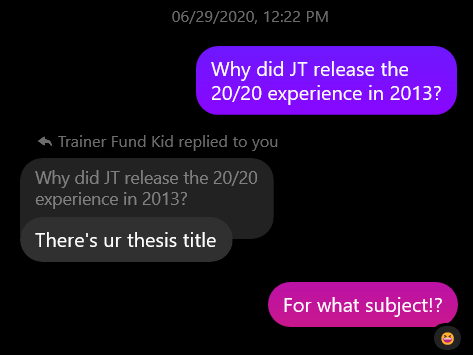
\includegraphics[width=.8\textwidth]{figures/working-title.png}
}
% \publishers{An Awesome Publisher}

%----------------------------------------------------------------------------------------

\frontmatter % Denotes the start of the pre-document content, uses roman numerals

%----------------------------------------------------------------------------------------
%	COPYRIGHT PAGE
%----------------------------------------------------------------------------------------

% \makeatletter
% \uppertitleback{\@titlehead} % Header
%
% \lowertitleback{%
% 	% \textbf{Disclaimer} \\
% 	% You can edit this page to suit your needs. For instance, here we have a no copyright statement, a colophon and some other information. This page is based on the corresponding page of Ken Arroyo Ohori's thesis, with minimal changes.
%
% 	% \medskip
%
% 	% \textbf{No copyright} \\
% 	% \cczero\ This book is released into the public domain using the CC0 code. To the extent possible under law, I waive all copyright and related or neighbouring rights to this work.
%
% 	% To view a copy of the CC0 code, visit: \\\url{http://creativecommons.org/publicdomain/zero/1.0/}
%
% 	% \medskip
%
% 	% \textbf{Colophon} \\
% 	% This document was typeset with the help of \href{https://sourceforge.net/projects/koma-script/}{\KOMAScript} and \href{https://www.latex-project.org/}{\LaTeX} using the \href{https://github.com/fmarotta/kaobook/}{kaobook} class.
%
% 	% \medskip
%
% 	% \textbf{Publisher} \\
% 	% First printed in May 2019 by \@publishers
% }
% \makeatother

%----------------------------------------------------------------------------------------
%	DEDICATION
%----------------------------------------------------------------------------------------

\dedication{\raggedleft\emph{To \_,\\
Something short and sweeet.}}

% \dedication{
% 	% The harmony of the world is made manifest in Form and Number, and the heart and soul and all the poetry of Natural Philosophy are embodied in the concept of mathematical beauty.\\
% 	% \flushright -- D'Arcy Wentworth Thompson
% }

%----------------------------------------------------------------------------------------
%	OUTPUT TITLE PAGE AND PREVIOUS
%----------------------------------------------------------------------------------------

% \includepdf[pages=1]{../MathSTICTemplate/main.pdf}

% Note that \maketitle outputs the pages before here
\maketitle

%----------------------------------------------------------------------------------------
%	PREFACE
%----------------------------------------------------------------------------------------

\begingroup

  %in the header, chapters start on any page to avoid too many blank pages
  \let\cleardoublepage\clearpage
  \pagelayout{margin}

\addchap{Abstract}

\addchap{Acknowledgments}

\addchap{How to Read This Thesis}

Use some words to talk about
\begin{itemize}
    \item lots of hyperlinking
    \item but not visible for readability
    \item example of \kl{bidirectional}
    \item in \cref{chap:formal-background}
    \item and emphasis like the following \intro{example}
    \item and even $\obsRef$.
\end{itemize}

Don't be confused, just click!

And also talk about the large margins, and fragments of the same figure like
\cref{fig:call-incr,fig:call-incr-fail}.

But still printable \textemdash{} colours are only (mostly?) used to aid readability.

\endgroup

%----------------------------------------------------------------------------------------
%	TABLE OF CONTENTS & LIST OF FIGURES/TABLES
%----------------------------------------------------------------------------------------

\pagelayout{wide}
\cleardoubleevenemptypage{}

\knowledgeconfigure{protect links}

\begingroup % Local scope for the following commands

\hypersetup{allcolors=.}

% Define the style for the TOC, LOF, and LOT
%\setstretch{1} % Uncomment to modify line spacing in the ToC
%\hypersetup{linkcolor=blue} % Uncomment to set the colour of links in the ToC
\setlength{\textheight}{230\vscale} % Manually adjust the height of the ToC pages

% Turn on compatibility mode for the etoc package
\etocstandarddisplaystyle% "toc display" as if etoc was not loaded
\etocstandardlines% "toc lines as if etoc was not loaded
\setcounter{tocdepth}{\sectiontocdepth} % Locally for the global toc

\tableofcontents % Output the table of contents

\setcounter{tocdepth}{\subsectiontocdepth} % To have correct tocs in the sections

% \listoffigures % Output the list of figures

% Comment both of the following lines to have the LOF and the LOT on different pages
% \let\cleardoublepage\bigskip
% \let\clearpage\bigskip

% \listoftables % Output the list of tables

\endgroup
\knowledgeconfigure{unprotect links}


%----------------------------------------------------------------------------------------
%	MAIN BODY
%----------------------------------------------------------------------------------------

\mainmatter % Denotes the start of the main document content, resets page numbering and uses arabic numbers

\selectlanguage{english}

\chapter{Introduction}\label{chap:intro}

\emph{“Our goal as computer scientist today, is to design the legacy systems of tomorrow.”}
\vspace{-1.5em}
\begin{flushright}
  \sidecite[][Timothy G.\ Griffin]{griffin2017legacy}
\end{flushright}

\margintoc%

\section{Context}

On the 1\nth{9} of July, 2024, 8.5 million Windows computers inside banks, airlines, TV
broadcasters, supermarkets and many other businesses suffered the infamous `Blue Screen of
Death' after (ironically) a faulty security update from cybersecurity
provider CrowdStrike was released.\sidecite[4\baselineskip]{verge2024crowdstrike}.

Even though it took only 78 minutes between when the issue was identified and
rectified, the ensuing chaos and disruption lasted hours if not days, as getting
the fix on affected machines and restarting complex systems was very difficult.
Although not as important as the human cost, the total finacial cost in terms
of downtime for businesses was estimated by one insurer to be between 5 and 9
billion USD.\sidecite{fitch2024crowdstrike}.

\begin{itemize}
    \item Explain \kl[OS]{operating system} and \kl{kernel} in lay terms.
    \item Explain \kl{systems programming language} in lay terms.
\end{itemize}

Whilst most of the commentary, including the root cause
analysis,\sidecite{rca2024crowdstrike} emphasised the need for better testing
and better deployment strategies, both of which are eminently sensible,
\emph{what} to test, and more importantly \emph{what's missing} in the tests
are only sufficiently clear with hindsight.

\emph{%
``The new IPC Template Type defined 21 input parameter fields, but the
integration code \ldots supplied only 20 input values to match against. This
\ldots evaded multiple layers of build validation and testing, as it was not
discovered during the sensor release testing process, the Template Type (using
a test Template Instance) stress testing or the first several successful
deployments of IPC Template Instances in the field.''
}

Aside from testing, Microsoft is also reported to be discussing locking down
access to the kernel with security vendors, and genereally designing it to be
more robust to rogue drivers and updates.

To me, the situation seems akin to building a wall with Swiss cheese, and when
something gets through, saying `we should have had more layers' or `layers
designed this way'. Surely one might wonder if we can consider a less porous
material?

So far, the answer has been no: methods for improving the reliability of such
software are \emph{costly}, mainly in terms of expertise, but also in term of
time and effort, with little scope for critical \emph{ongoing} maintenance. And
whilst the exact contributions of this thesis would not have prevented
CrowdStrike (even hinting at that would be temeritous), they are extremely
relevant to the general domain.

This thesis argues that the answer is now a \emph{qualified yes}. A `less
porous material' is possible with what we know now, and not too complex
conceptually (though novel in its application). The main challenges come due to
\emph{scale}. Whilst the cost of the technology is still too high for mass
deployment, the trend is downward and should continue that way with sustained
effort.


\section{Thesis statement}

In this thesis, I will argue that building a verification tool for C, suitable
for handling lowl-level systems programming idioms, is two parts engineering,
and one part theory. Little of the theory are novel or complex, but its
application at scale present new challenges and insights. The proportions do
not correspond to three different topics, which fit neatly in either bucket.
Rather, each conceptual part of this thesis has varying mix of those
categories, which I will explain later in \nameref{sec:contributions}.

To put those parts into context, I first need to explain the role and quirks of
the venerable C programming language, and the relevant developments in
verification theory.

\section{The C Programming Language}

\begin{itemize}
    \item More than fifty years after its introduction, and despite competition
        from C++\sidecite{isocpp1998} and Rust\sidecite{rust}, C remains in common use.
    \item Initially designed for portability, relative simplicity (but with plenty of
        subtlety around pointers), ease of compilation, proximity to hardware/control, was simple back then.
    \item Two forces: portable (underspecified for freedome), optimise (because performance critical code)
            have evolved it.
    \item Is the primary language of the Linux kernel.
    \item Is it really easy to compile though? Alias analysis, pointer rules.
        Provenance examples and optimisation issues here.
    \item Is it really so simple? Shifts burden from compiler writer to the programmer.
    \item ISO standard vs.\ de facto C\@. Consensus artifact hence not simple (lots of stakeholders).
    \item \kl{Cerberus} executable and \emph{empiricaly validated} semantics.
    \item Maybe some sort of list append example?
\end{itemize}

\section{Verification with Separation Logic}

\begin{itemize}
    \item Floyd and Hoare, key ideas in the 1960s.
    \item People tried to use this and failed (Euclid system for Pascal).
    \item Specifications of pointers because of aliasing issues, $n^2$ no aliasing conditions,
        do not compose well ${(n + m)}^2$ conditions.
    \item Key breakthrough, John Reynolds and Peter O'Hearn
    \item Frame rule (and the name comes from AI, asserting facts modularly, frame problem)
    \item This enables working with pointers and heap objects.
    \item Pen and paper proofs about sequential (then concurrent imperative programming, Iris?).
    \item Continue with list append example?
\end{itemize}

\section{CN:\ C, No bugs!}

Before I explain how \intro{CN}\sidenote{`\kl{CN}' does not stand for anything; its name is
a historical accident.} \emph{works}, I will explain how it is \emph{used}.

\kl{CN} is a program, which, in its \intro{proof mode}\sidenote{There are other
modes to CN, most notably instrumentation and test generation, which I will
mostly ignore.} given a C file, ensures that (a) the input code is free of
undefined behaviour and (b) correctly implements any specification written in
\intro{annotations} in comments demarcated by \cinline{/*@} and \cinline{@*/}
(so that they are first and foremost, for almost all C tools, a regular C
comment). Importantly, for compositionality, performance (paralellisability),
and ease of annotation,\sidenote{Annotations follow the structure/units of the
program.} these are checked on a \intro{per function} basis.

This means that even in the absence of annoations, code is being checked for
undefined behaviour. Incrementing an unsigned integer is perfectly acceptable
\begin{figure}[h]
\centering
\cfile{code/unsigned_increment.c}
\caption{Example unsigned\_increment.c.}\label{fig:un-incr}
\end{figure}%

\ldots but incrementing a signed integer triggers an error message.%

\begin{figure}[h]
    \centering
    \cfile{code/increment_broken.c}
    \caption{Example increment\_broken.c.}\label{fig:incr-broken}
\end{figure}

The wording of the error message is inherited from \kl{Cerberus}, and shows its
origins as a formal, executable specification for \kl{ISO} and \kl{de facto}
\kl{C}. In particular, it points to the relevant section of the standard which
has been violated, and uses jargon (``exceptional condition'') to indicate that
there are values of \cinline{x} for which executing this function would result
in \kl{UB}. Because of the \intro{per function} checking, the violation is not
guaranteed, but \emph{possible}. Specifically, it is considered an error
because there exist values, which if used to call this function, would result
in \kl{UB}. Phrased differently, it is the combination of the absence
\kl{annotation}s constraining the input, \emph{with respect to} what the body
of the function does with those inputs, which is erroneous.

Admittedly, as we shall discuss in \cref{sec:error-msgs}, there is much room
for improvement to take the language of the \kl{standards committee} and
translate it into something suitable for mere mortals. Yet the source location
and the \intro{state file} it points to is helpful. If \kl{proof mode} fails
because \kl{CN} was not able to prove a constraint, it produces a
\kl{counter-example} with values assigned (see \cref{sec:counter-ex})
internal representations of program variables.

\begin{figure}[h]
    \centering
    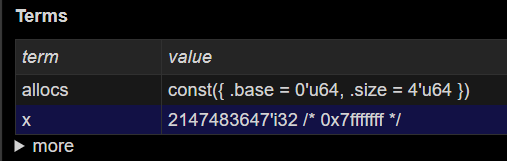
\includegraphics[width=.8\textwidth]{figures/increment_broken_state.png}
    \caption{Counter example for increment\_broken.c.}\label{fig:incr-broken-counter-ex}
\end{figure}

We can avoid this error by constraining the values of the input with a
precondition annotation as follows.

\begin{figure}[h]
    \centering
    \cfile{code/increment.c}
    \caption{Example increment.c.}\label{fig:incr}
\end{figure}

Here we see the keyword \cinline{requires} is used to introduce a pre-condition
on the input. \cinline{MAXi32()} is an in-built function which represents the maximum
value a signed 32-bit integer can represent. By constraining the input so that
it is strictly less than the maxiumum value, the function is now guaranteed to
have no \kl{UB} for all its inputs, no matter what the context. This is because
whilst pre-conditions are \emph{assumed} inside the function, they are
\emph{required} when calling it.

\begin{figure}[h]
    \centering
    \cfile{code/call_increment.c}
    \caption{Example call\_increment.c.}\label{fig:call-incr}
\end{figure}

In the first example, we see that from the constraint \cinline{y <=
100i32},\sidenote{Integer literals are currently written with a type
annotation, similar to Rust.} \kl{CN} deduces that \cinline{y <=
MAXi32()}\sidenote{Foreshadow subtyping, and bidirectional things.} and permits
the call to \cinline{increment}. Conversely, \cinline{INT_MAX} does not meet
that constraint, and so CN raises an error.

\begin{figure}[h]
    \centering
    \cfile{code/decrement_broken.c}
    \caption{Example decrement\_broken.c.}\label{fig:decr-broken}
\end{figure}

However, if we try to decrement the result of the successful call, \kl{CN}
raises an error. This is because that \kl{CN} has no indication on the
constraints of the return value (other than those deduced from its C type,
namely that it fits within a signed 32-bit integer).

\begin{itemize}
    \item Pointers
    \item User defined predicates
    \item Array example
\end{itemize}

\begin{marginfigure}
  \ContinuedFloat*
  \begin{mathpar}
      \inferdef{Var}{\vdash{} \Gamma{} \\ (x: A) \in{} \Gamma{}}{\Gamma{} \vdash{} x \ty{} A}\label{rule:cic-var}
  \end{mathpar}
  \caption{Integrate Ott into this system.}\label{fig:cic-var}
\end{marginfigure}

Reference the rule: \ruleref{rule:cic-var} opposite.

\begin{marginfigure}
\ContinuedFloat{}
  \begin{mathpar}
      \inferrule{\Gamma{} \vdash{} A \ty{} \uni{} \\ \Gamma, x: A \vdash{} t \ty{} T}
      {\Gamma{} \vdash{} \l x: A.\ t \ty{} A \to{} T}
    \and
    \inferrule{\Gamma{} \vdash{} f \ty{} A \to{} T \\ \Gamma{} \vdash{} u \ty{} A }{\Gamma{} \vdash{} f\ u \ty{} T}
  \end{mathpar}
  \caption{Ott in here too.}\label{fig:cic-nondep-fun}
\end{marginfigure}

You can see more at work in \cref{fig:cic-nondep-fun}.

\section{Contributions of this thesis}\label{sec:contributions}

\subsection{Formalisation of CN}

Kernel CN (type safety), the gap between CN and this (inferring output
arguments, historical note on inferring indices), heap factoring, and Ott
engineering.

\subsection{Design, formalisation and implementation of CN-VIP}

Memory object model and adapting it to CN

\subsection{Will the real world C, please stand up?}

Tree Carver (preprocessor), buddy allocator update, issues/pain points (on
GitHub repo), working with Galois.

\begin{comment}

\emph{“\kl{Coq} is an old man now, and it has a lot of scars.”}
\vspace{-1.5em}
\begin{flushright}
  \sidecite[][citing Assia Mahboubi]{QuantaPA}
\end{flushright}

\margintoc[4em]

This thesis belongs to the domain of \kl[dependent type]{type theory},%
\sidenote{If you do not know what this or any other word in this introduction
means, read on! They will be explained in due time.}
itself at the crossroads between computer science and mathematical logic.
One of the field’s goals is to give theoretical and practical foundations
for software tools helping humans in constructing and verifying proofs –
in the mathematical sense.
Such tools are called \kl{proof assistants}, and \kl{Coq}, the one
on which my work was mainly focused, is central in this thesis.

Over their more than 50 years of existence, proof assistants have
turned into an established technology. This history is both a blessing and a curse: as
the field matured, the tools have become more and more complex, making them more and more
powerful, but also more and more prone to critical bugs hiding in dark corners. At a time
when they are gaining traction in an increasing number of communities
concerned with high trust levels, this simply cannot be.
The historical solution of keeping a small, trusted \kl{kernel}
– the so-called De Bruijn criterion –
is not enough if we wish to keep moving on and integrate new, powerful features
to keep up with the needs of users.

There is a straightforward solution to this:
proof assistants have been used for decades to certify programs correctness.
Why could they not prove \emph{themselves} correct? After all, if this is
the gold standard we demand for software, it should apply first and foremost to the ones
used to justify that trust. For the proof assistant \kl{Coq},
this is the ambition of the \kl{MetaCoq} project,
which aims at providing a drop-in replacement for \kl{Coq}’s \kl{kernel} that has been
proven correct,
even though it handles all the subtleties and quirks of said \kl{kernel}.
No more trusting a complex and ever-evolving implementation, trust the formally validated
\emph{proofs} instead!

But before we can hope to achieve that goal, we need a deeper study of the structures at work
in the \kl{kernel}. In particular, its typing algorithm is \emph{bidirectional}, meaning that
it constantly alternates between the two problems of type \emph{inference} –
finding a type for a term – and type \emph{checking} –
verifying that a type is adequate for a term. While this
structure is crucial in relating the specification of the type system to its implementation,
it has been rather little studied in the context of the
\kl{Calculus of Inductive Constructions} (\kl{CIC}),
the theoretical foundation of \kl{Coq} – but also of the closely related
\kl{Lean}, \kl{Agda}…

This thesis aims at filling that gap, by providing a thorough study of bidirectional \kl{CIC},
formalized in the framework offered by \kl{MetaCoq} project. This is a key
ingredient in the first formal proof of soundness and completeness of a type-checking
algorithm for a realistic proof assistant kernel.
It was also able to uncover bugs in \kl{Coq}’s kernel that had gone unnoticed until then.

But bidirectional typing is also an interesting theoretical tool in its own right,
giving a valuable form of control over computation.
In particular, it is a necessary piece in the design of a gradual extension of
\kl{CIC}, \kl{GCIC}.
\kl{Gradual typing} aims at bringing to programmers both the flexibility of
development offered by dynamic typing, and the strong guarantees given
by static typing, in one and the same system. \kl{GCIC} intends
to bring that flexibility to dependently-typed programming,
and, by using the power of the \kl{Curry-Howard correspondence}, to proof writing.
But this endeavour comes with subtle difficulties,
that can only be solved in a bidirectional setting.

To replace this work in its larger context, this introduction begins with a very
short history of mathematical logic (\cref{sec:logic-history}), which exposes the
main questions of that field. Follows a presentation of the links between logic and
computer science, through \kl{proof assistants} (\cref{sec:proof-assistants}).
Next, \cref{sec:intro-coq-en} focuses more closely on presenting
the research questions I worked on: bidirectional typing, \kl{MetaCoq} and gradual typing.
Finally, \cref{sec:this-thesis} summarizes my contributions to these questions.

\section{A Very Short History of Logic}
\label{sec:logic-history}

\subsection{Syllogisms}

The main question that logic seeks to answer is that of finding criteria in order to determine
if a reasoning is valid. In Western tradition, this challenge can be traced back to the
Antiquity, and particularly to Aristotle's \textit{Organon}.
The main contribution of this work is to introduce the notion of syllogism.
These are simple fragments of reasoning, whose validity stems from the
fixed structure they follow, rather than a specific content.%
\sidenote{The most well-known is probably the \textit{Barbara} syllogism, and example
of which is: \emph{all humans are mortals; Socrates is human; so Socrates is mortal.}}
If complex reasoning is built from assembling such syllogisms, it must necessarily be valid as
a whole, since every assembled fragment is. There are two important ideas at work here.

The first is that reasoning can be valid or not, depending only on its structure,
independently of its content.
It can be syllogisms, but many other systems. We will come across a certain number of them
in this thesis!

The second idea is that of a construction from elementary components.
Starting from a set of rules
we have identified as valid \textit{a priori}, we have a means to ensure the validity
of potentially very complex reasoning: it suffices to check that these
can be decomposed into the base components.

For the Greek philosophers, logic was also conceived as a means towards communication.
The aim was to check one’s own reasoning, but also to be able to convey
it, by fixing a logical formal system.%
\sidenote{Structural rules reasoning should obey, as those of syllogisms.}
A person wanting their conclusion to be accepted by others would only have to express their
reasoning in a perfectly precise way in the framework of such a formal system.

From that point on, the main focus of logic as a discipline
concentrates on this structure which underlies reasoning.
The main challenge is to construct a formal system, adapted to a specific
field of reasoning. In the case we are interested in, mathematical logic, this
allows us to give a precise meaning to what constitutes a valid mathematical proof.


\subsection{The beginning of mathematical logic: towards a formal foundation}[Towards a formal foundation]

Following Aristotle, mathematicians seized logic in order to build a formal system
able to serve as a rigorous foundation for mathematics.
The links between logic and mathematics go back to Greek Antiquity, but
mathematical logic as a standalone discipline really established itself
during the 19\textsuperscript{th} century, thanks to important progress on two main aspects.

The first consisted in freeing mathematical logic from natural languages%
\sidenote{By opposition with the formal languages which appear in mathematics,
  computer science, etc.},
unsuited to a formal description of reasoning, and to instead design a new specific
form of language that could serve as a basis for mathematical reasoning.
An important step here was \citeauthor{Begriffsschrift}'s
\citetitle{Begriffsschrift}~\sidecite{Begriffsschrift}, which, for the first time,
gave a formal language rich enough to express mathematics satisfyingly. Its
major addition was the notion of quantifier, essential to the mathematical vernacular,
as they give a faithful way to account for universal%
\sidenote{For instance: “Every even natural number is the sum of two prime numbers”.}
and existential%
\sidenote{For instance: “There exists a real whose square is 2”.}
properties.

The second aimed at showing that mathematics as a whole could be reconstructed from a
few simple properties. An important step was the reduction of analysis to the properties
of real numbers, followed by constructions of those from arithmetic given almost
simultaneously by – among others – \sidetextcite{Dedekind1872} and
\sidetextcite{Cantor1872} in 1872.
Meanwhile, \sidetextcite{Peano1889} proposed an axiomatization of natural numbers close to the
one still used today. Finally, Cantor again proposed set theory \sidecite{Cantor1883}
as a formalism expressive enough to describe all mathematical object as sets of elements.

\subsection{The foundational crisis of mathematics}[The foundational crisis]

Unfortunately, the system proposed in the \citetitle{Begriffsschrift} is inconsistent!
That is, it is possible to use it to prove falsity, 
making the logical system collapse.%
\sidenote{In a system where falsity is provable, all propositions are,
  which is known as the principle of explosion.
  Such a system, where everything – and its negation – is provable can obviously not
  serve as an adequate foundation for mathematics.
}
This result, due to Russell%
\sidenote{%
  In a letter to Frege in 1902 the latter made made public
  in \textcite[Nachwort p.~253]{Frege1903}.}%
\margincite{Frege1903}
marked the opening of a crisis period.
Indeed, it cast doubt upon the systems that had started to establish
themselves as good candidates to serve as foundations – that of Frege, but
mainly those of Cantor, which were affected by the same difficulties.

A possible solution has been suggested ten years later  by \citeauthor{Whitehead1913} in their
\citetitle{Whitehead1913} \sidecite{Whitehead1913}. This colossal piece of work
not only proposed a formal system avoiding the inconsistency
of \citetitle{Begriffsschrift}. It also built a significant amount
of mathematics in this system, including a construction of integers,
some arithmetic, and finally real numbers.

In parallel, in the continuity of Cantor’s work, \sidetextcite{Zermelo1908} and others
worked towards giving a version of Cantor’s set theory that is consistent. This lead to what
is colloquially referred to as Zermelo-Fraenkel set theory – ZF, or ZFC when the
axiom of choice%
\sidenote{An axiom very useful in numerous branches of mathematics, but which is often treated
separately, as it is both less crucial than the other axioms of ZF and at the root of
counter-intuitive results.}
\sidecite{Zermelo1904} is added –, which also seemed able to serve as a
solid foundation for mathematics.

\subsection{Incompleteness}

The search for a formal system adequate as a foundation for mathematics however hit a
second major difficulty: Gödel’s incompleteness theorem \sidecite{Goedel1931}. It asserts
that a formal system in which one can construct integers such as those of Peano – and so
\textit{a fortiori} any system rich enough to serve mathematician’s needs – cannot
prove its own consistency.%
\sidenote{Unless the system is inconsistent, in which case it can prove \emph{everything},
by virtue on the explosion principle, including its own consistency… and inconsistency!}
Thus, no formal system can serve as a basis for mathematics
with a formal certitude as to its adequacy.
Indeed, as we cannot prove the consistency of the system in itself, it could very well
turn out to be inconsistent, ruining all the efforts put into its use – just like what
happened with Frege’s \citetitle{Begriffsschrift}. And if we were to use a second system
to prove the first consistent, we would only shift the prolem: now we rely on the
consistency of the second system.

A consequence of this theorem is that a system rich enough to found mathematics is
necessarily incomplete.%
\sidenote{%
  This means that there exist independent statements, that is assertions which
  cannot be proven, and whose negation cannot be proven either.
  The consistency of the system under consideration is one example of such a statement.
}
Thus, in what follows, I will never refer to truth in an absolute sense – which could
only be meaningful in a complete system where every statement is true or false –, but
only about provability \emph{relatively to a given system}.

\subsection{A satisfactory situation?}

Despite the difficulties put into light in the beginning of the 20\textsuperscript{th}
century, the research in mathematical logic reached a somewhat satisfactory situation
a few decades later.
First, ZFC is a reasonable formal system on which mathematics can be founded. Moreover,
the mathematical community is overall convinced it would be \emph{theoretically} possible
to write down all mathematics using ZFC\@. This is enough for most of its members,
even if those who attempt to actually give it a try, in the vein of the
\citetitle{Whitehead1913}, are quite few.

In \emph{practice}, however, things are very different. The human development and
verification of formalized mathematics%
\sidenote{%
  That is, effectively expressed in a fixed formal system.}
seems both impossible, and unnecessary.
On the one hand, it would demand a considerable effort, because such mathematics would
require an extremely high level of precision, both from the author of the formal proof
and from the reader. At the same time, this would not significantly reduce the risk of
errors. It would indeed be very hard for humans to check that some reasoning doubtlessly
follows the rules of the system: a tiny error can easily creep inside thousands of pages
of formal reasoning. Finally, describing mathematics in this way would drown the vital
mathematical intuitions, making communication sterile.

If we wish to make formal mathematics practicable, and benefit from the guarantees
they bring while eliminating these crippling defaults, we thus need new tools.

\section{Computers Enter the Scene}
\label{sec:proof-assistants}

A new element however radically modifies the previous situation: the advent of computers.
Indeed, computer science provides new tools, making formalized mathematics both possible
and attracting.

\subsection{Proof assistants}

Computers excel where humans are weak: their speciality is to treat large volumes of
information in a very precise way, exactly the kind of needs brought up when manipulating
formalized mathematics. Therefore, already at the beginning of the 70s,%
\sidenote{With systems like Automath \cite{DeBruijn1970}, or Mizar
  \cite{Rudnicki1992}.}%
\margincite{DeBruijn1970}%
\margincite{Rudnicki1992}
software tools, collectively called \intro{proof assistants}, start to
appear, that are dedicated to writing and verifying formal proofs.
Through the formalization of proofs and the verification by computers that they
actually follow the rules of the underlying logical system, proof assistants open the
door to a level of trust much higher than that allowed by “informal” proofs.
Renowned mathematicians, such as \sidetextcite{Voevodsky2010},
\sidetextcite[][Preface, p.\ xi]{Hales2012}, or \sidetextcite{Scholze2021} have indeed
turned to proof assistants, particularly in order to lift uncertainties regarding the
solidity of their own work.

Moreover, proof \emph{assistants} are not simply proof checkers: beyond verification,
they supply users with a large range of tools to ease the conception of
formal proofs. These tools allow users to write proofs at a
high level, and in an interactive manner,%
\sidenote{In most modern proof assistants, the final proof is built as the result of
  an exchange between the programmer and the tool, rather than written as a single block.}
leaving it to the proof assistant to construct the formal proofs.
They range from simple facilities, such as the possibility to visualize the structure
of proofs, or the tracking of hypotheses, to much more ambitious techniques.

Indeed, computer science lets us automatize entire parts of
proof writing, for instance through the use of tactic languages \sidecite{Delahaye2000},
with which one can program proof generation.
In addition, the automatic construction of proofs is a research field by itself,
and the question of its integration intro proof assistants is an active topic
\sidecite{Blanchette2016,Ekici2017}. Computer science has also proven its worth in the
setting of mathematical computations (computer algebra systems, numerical analysis),
and here again promising interactions with proof assistants are starting to arise
\sidecite{Lewis2022,Mahboubi2019}.

Finally, if the use of software eases the writing of proofs, proof assistants conversely
open new possibilities for programming. They indeed offer a natural framework to describe in
the same place the source code of a program, its specification, and the formal proof that the
former fulfils the latter. This way, we can \emph{prove} that the program runs correctly,
without encountering any bugs.
This mathematical certainty is much more reliable than any test set!
In this field, numerous projects have already achieved large scale programs, entirely proven
correct: compiler for the C language \sidecite{Kaestner2017}, implementation of the
\textsc{Https} protocol \sidecite{Bhargavan2017}, differential equations solving
\sidecite{Immler2018}…

\subsection{Logic, Programming and Type Theory}

In order to work, proof assistants must be founded on a formal system, corresponding to
the “rules” of the mathematical “game” they are supposed to enforce.
Thus, they require a renewed study of mathematical logic, but with the practical aim of
building tools that are at the same time powerful and easy to use.
There are multiple families of proof assistants, based on very different formal systems.
The one I am interested in in this thesis relies on the \kl{Curry-Howard correspondence}
and \kl[dependent type]{dependent type theory}. The proof assistant \kl{Coq}
\sidecite{CoqDevelopmentTeam2022}, which is at the heart of my work, belongs to this family.

If one compares a computer program with a text in a natural language,
\intro(en){types}
are a kind of equivalent of grammatical categories. However, contrarily to natural
languages, these types are conceived at the same time as the programming language, in order
to mirror properties of the objects it manipulates.
Their first use is to detect manifest errors. For instance, if a procedure
intended for an object of type “image” is applied to an object of type “character string”,
an error can be reported to the programmer.%
\sidenote{A well-known slogan due to \textcite{Milner1978} claims that
“Well-typed programs cannot go wrong.”}%
\margincite{Milner1978}
But types are very versatile, and their capacity to encode properties of the underlying
programs can be used for compilation, documentation, and many other applications. In our
framework, for instance, types correspond to the validity of a logical reasoning.

This idea is that of the \intro{Curry-Howard correspondence}.%
\sidenote{Made explicit for the first time in informal notes by Howard dating back to 1969,
but published only much later \cite{Howard1980},
themselves based upon previous remarks by Curry \cite{Curry1958}.}%
\margincite{Howard1980}%
\margincite{Curry1958}
Rather than a precise theorem,
it is more of a very general concept, according to which two worlds closely resemble each
other: on the one hand, that of logic and proofs, on the other that of programs
and their types.

\begin{marginfigure}

  % \begin{mathpar}
  %   \inferrule{ \Gamma, A \vdash B}{\Gamma \vdash A \Rightarrow B} \and
  %   \inferrule{\Gamma \vdash A \Rightarrow B \\ \Gamma \vdash A}{\Gamma \vdash B} \and
  %   \inferrule{\Gamma, x : A \vdash t : B}{\Gamma \vdash \lambda x : A . t : A \to B} \and
  %   \inferrule{\Gamma \vdash f : A \to B \\ \Gamma \vdash u : A}{\Gamma \vdash f~u : B}

  % \end{mathpar}

  % \caption{Règles d’inférence pour l’implication et de typage des fonctions}

  \begin{mathpar}
    \inferrule{A \\ B}{A \wedge B} \and
    \inferrule{A \wedge B}{A} \and
    \inferrule{A \wedge B}{B} \\
    \inferrule{a \ty A \\ b \ty B}{(a,b) \ty A \times B} \\
    \inferrule{p \ty A \times B}{p.1 \ty A} \and
    \inferrule{p \ty A \times B}{p.2 \ty B}
  \end{mathpar}
  
  \caption{Inference rules for conjunction and typing rules for pairs}
  \label{fig:curry-howard-example-en}
\end{marginfigure}

A short example says more than a long abstract talk, so let’s look at the correspondence
at work in \cref{fig:curry-howard-example-en}, in the form of inference/typing rules:
each bloc presents a rule, with above the bar the hypotheses, and below the conclusion.
The first three rules govern the logical conjunction “and”, written $\wedge$.
The first means that to deduce the proposition $A \wedge B$ (“$A$ and $B$”), it is enough
to deduce $A$ and $B$ taken individually.
Conversely, if we have as hypothesis $A \wedge B$, then we can deduce both $A$ (second rule),
and $B$ (third rule).
The last three rules govern typing%
\sidenote{Written using a colon.}
for the pair type $A \times B$. A pair $(a,b)$ built
from a first object $a$ of type $A$ and a second object $b$ of type $B$ has type $A \times B$.
Conversely, if $p$ is a pair of type $A \times B$, then we can retrieve its first component
$p.1$, which is of type $A$, and its second $p.2$, of type $B$.
If we erase the terms%
\sidenote{In the context of type theory, we often talk about \emph{terms} instead of programs,
  but the two are synonyms.
}
of the bottom rules, we obtain \emph{exactly} the rules above!
Thus, the programming construct of pairs corresponds to the logical concept of conjunction.

This extends well beyond the specific case of conjunction, in a general correspondence
between, on one side, logical propositions and their proofs, and, on the other, types and programs.
We can see properties as types, and a proof of a given property as a program of the
corresponding type – or the other way around!
Beyond a simple analogy between formalisms of different origins, this correspondence
is a powerful tool to establish a dialogue between two worlds. In particular, it
relates two \textit{a priori} quite distant problems: checking that a proof
is valid, and checking that a term is well-typed. In both cases, it amounts to checking that
a construction – program on one side, proof on the other – respects a set of formal
rules guaranteeing it is well-formed.

The \kl{Curry-Howard correspondence} is therefore ideal to serve as a foundation for
\kl{proof assistants}, since it gives access, when studying formal logical systems,
to the rich literature on programming languages, in particular on the theory and
implementation of types. In this framework, the
\intro[dependent types]{dependent type systems} are a specific family of type systems,
whose main characteristic is the ability for types to depend on terms. The archetypical
example from the point of view of programming is the type $\Vect(A,n)$
of vectors of length $n$. These are lists that contain exactly $n$ elements of type $A$ – with
$n$ a natural number.
This type depends on $n$, in the sense that the type’s inhabitants differ depending on the
integer’s value.
From the point of view of logic, this dependency corresponds to quantification: if we
wish to express a universal property “for all $x$, the property $P(x)$ holds”, then we need
the property $P$ to depend on $x$.
Thanks to this ability to express quantification, dependent types are rich enough
to serve as foundations for mathematics.

\section{\kl{Coq} and Its Kernel}
\label{sec:intro-coq-en}

Let us now focus a bit more on the proof assistant which we will consider mainly in this
thesis: \kl{Coq}.

\subsection[The kernel]{The kernel, cornerstone of the system}

\begin{figure}[h]

  \centering
  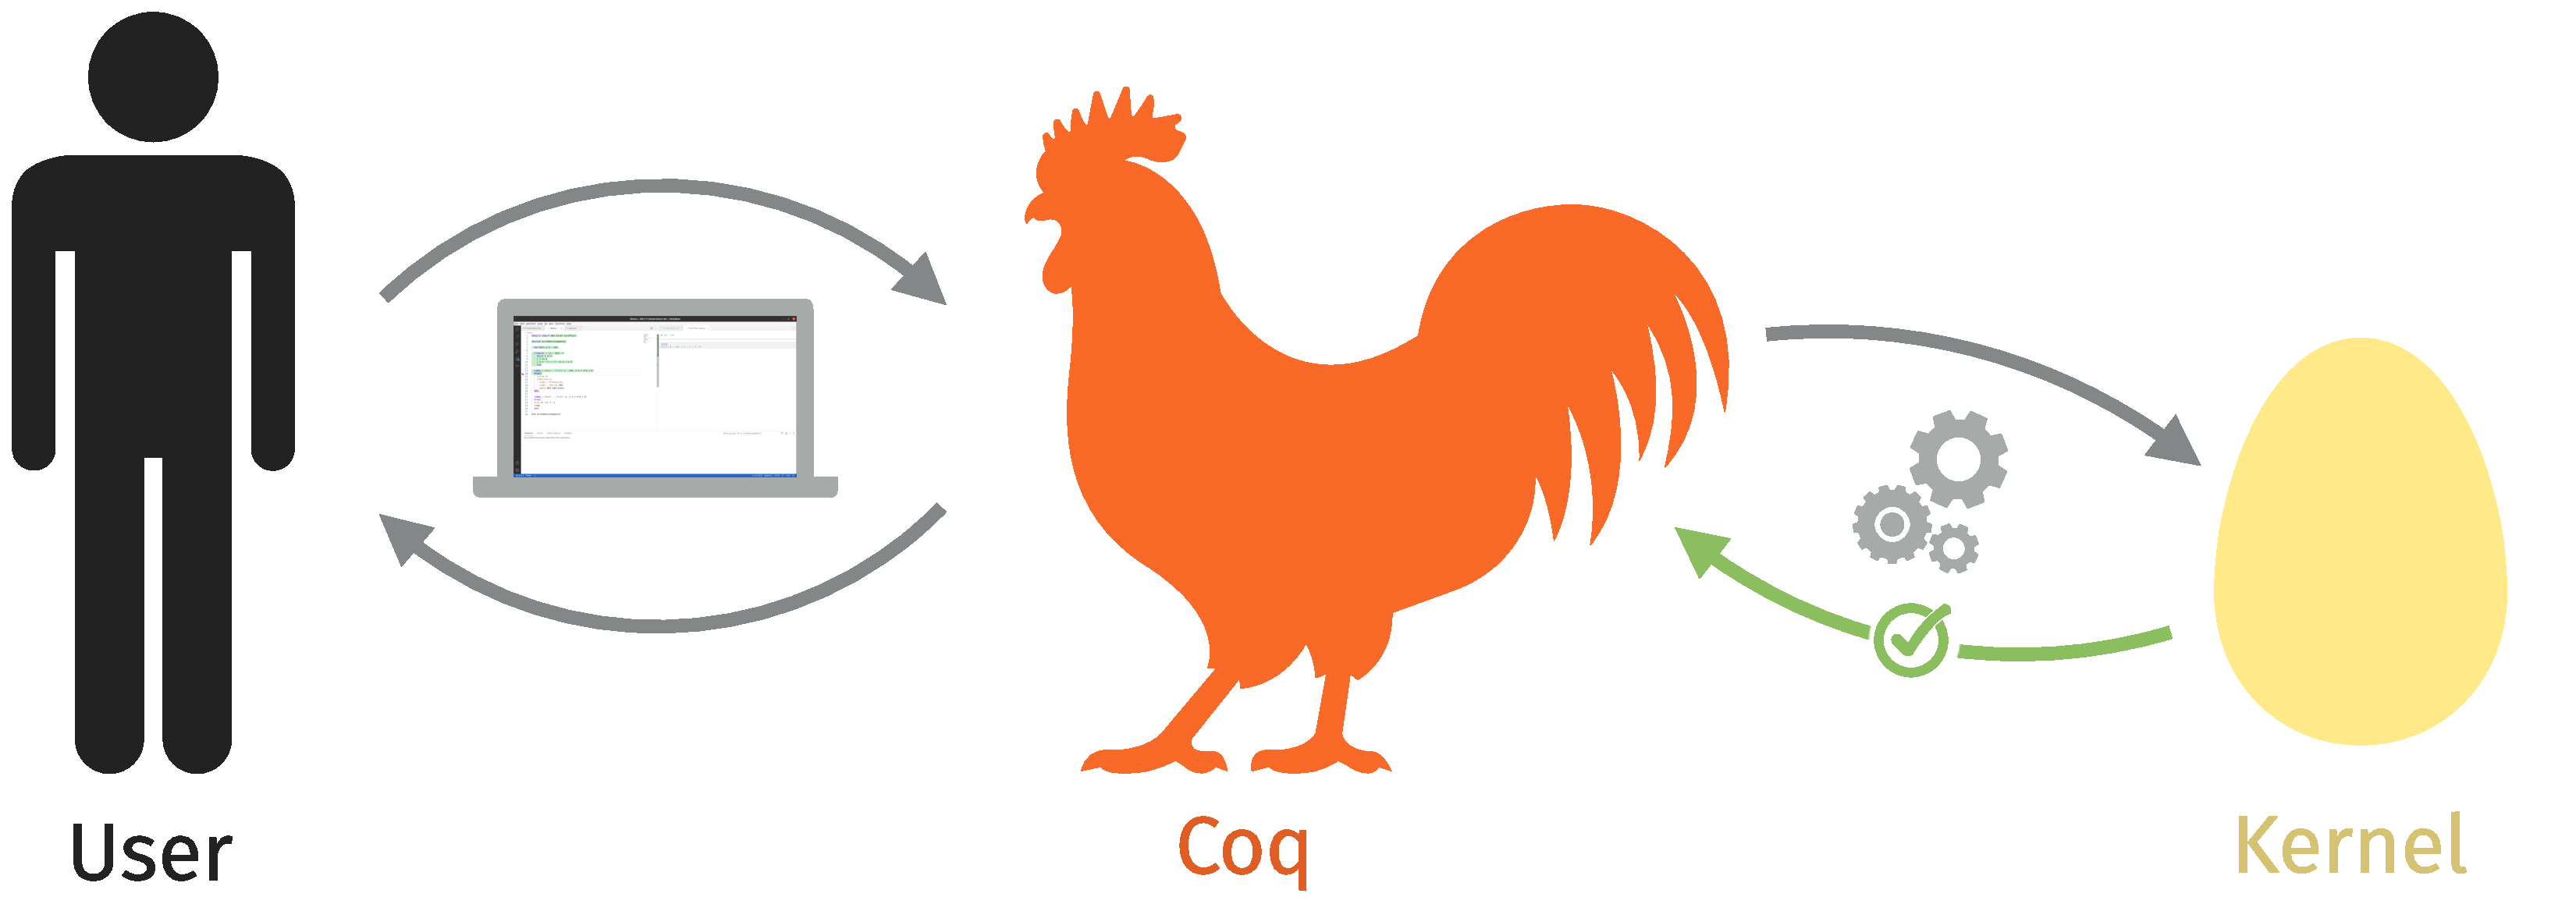
\includegraphics{./figures/coq-kernel-en.pdf}

  \caption{\kl{Coq}’s schematic architecture}
  \label{fig:coq-en}
\end{figure}

\kl{Coq} is based on the \kl{Curry-Howard correspondence}: proofs are seen as programs,
in a language called \intro{Gallina}, and their verification is done using an algorithm
close to those used for types in conventional languages. However, if, in the first versions
from the 80s, \kl{Coq} proof were mostly written directly in \kl{Gallina}, it is
no longer the case at all. The reason is that the major part of the tool in its
current versions aims at helping the user in generating a correct proof. It is a true
\kl[proof assistant]{proof \emph{assistant}}!
The way \kl{Coq} works is illustrated in \cref{fig:coq-en} : the user interactively exchanges
with \kl{Coq}, which uses this interaction to generate a proof term. This proof term is then
sent to a very specific part of the tool, called the \intro{kernel}.
This is the part implementing the type-checking algorithm, and thus responsible for ensuring
that the proof terms built interactively are correct.
The \kl{kernel} is thus the crucial part of \kl{Coq}, because it is the one – and only –
ultimately responsible for proof-checking.
This architecture, which clearly isolates the critical part of the system, is called
\intro{De Bruijn criterion} \sidecite{Barendregt2001}, in tribute to one of the pioneer
of proof assistants.

If the rest of the ecosystem has grown much more than the \kl{kernel} since the beginning,
the latter has also evolved, becoming gradually more complex.
And, as any other software development, it is not safe from bugs.%
\sidenote{The magnitude is that of one critical bug found every year, a list is maintained
at the following address: \url{https://github.com/coq/coq/blob/master/dev/doc/critical-bugs}.}
These are in general hard to exploit for a user, even more so without noticing.
But still, they exist, and since the \kl{kernel} tends to get more and more complex, they
are likely to continue appearing.

\subsection{\kl{MetaCoq}, a formalization in \kl{Coq}, for \kl{Coq}}[\kl{MetaCoq}]
\label{sec:intro-metacoq-fr}

If we wish to guarantee a trust level as high as possible in the \kl{kernel}, we must
resort to new ideas. This is what the \kl{MetaCoq} project is all about. The idea
is simple: use \kl{Coq} itself to certify the correctness of its \kl{kernel}.

More precisely, the first step is to describe formally the type system on which the \kl{kernel}
is based, and to show its theoretical properties.
This is already a difficult endeavour: in order to ease its use, \kl{Coq}’s type theory
incorporates a lot of complex features.

Once this meta-theory is established, the second step
% \sidenote{This is the one on which I mostly work, and on which we will come back in more
% length later on.}
consists in implementing a type-checking algorithm as close as possible to the one of the
\kl{kernel}, directly in \kl{Gallina}%
\sidenote{Indeed, thanks to the \kl{Curry-Howard correspondence}, \kl{Gallina} is not
only a proof language, but also a true programming language!}.
We show, while defining the algorithm, that it is indeed \reintro(bidir){sound}%
\sidenote{If the algorithm claims that a term is well-typed, then it is the case.}
and \reintro(bidir){complete}%
\sidenote{The algorithm answers positively on all well-typed programs.}.
Together, these two properties correspond to the \intro(bidir){correctness} of
the program.

Finally, in a third step, we extract out of this certified \kl{Gallina} program another
more efficient program, by erasing the content related to the proof of correctness, in order
to keep only the algorithmically relevant one.
This extraction is a complex but crucial step if we wish to replace the current \kl{kernel}
while keeping a reasonable efficiency. Therefore, we also prove that said extraction
is correct,%
\sidenote{Meaning that it preserves the semantics of programs.}
once again by programming it in \kl{Gallina}.

\subsection{Checking, inference and bidirectional typing}[Bidirectional typing]

While proving the correctness of the type-checker is relatively easy once the
meta-theoretical properties of the type system have been established, completeness is harder.
In order to prove it, it is very useful to go through an intermediate specification,
which is more structured than the theoretical one.
In particular, it is important to separate two close but distinct questions:
on the one side, type-checking, where we \emph{check} that a term indeed has a
given type;
on the other side, inference, where we try and \emph{find} a type for a term, if such a
type exists.
The typing algorithm of \kl{Coq}'s \kl{kernel} is \intro{bidirectional}, meaning that it
alternates constantly between these two processes when it checks that a term is well-typed.
Describing this bidirectional structure independently of the algorithm allows for a
clear separation between, on the one side, its equivalence with the original specification,
and, on the other, the part purely dedicated to implementation questions.

In the specific case of dependent types, even if present in type-checking algorithms since
the origin – see \eg \sidecite{Huet1989} –, bidirectional typing has been relatively little
studied. However, beyond its strong relation to algorithms, this approach also presents
theoretical advantages: its more constrained structure makes it easier
to obtain properties that are difficult to obtain in the standard context.

\subsection{Gradual types: some flexibility in a desperately static world}
  [Gradual types]
\label{sec:intro-graduel-en}

There are two main approaches to program type-checking. In the static approach,%
\sidenote{On which \kl{Coq} is based.}
types are verified prior to the execution, whereas, in the dynamic approach, the well-typedness
of operations is verified on the fly during that same execution.
The dynamic discipline is more flexible, as it checks exactly what is necessary
for the good execution of a program.
The strictness of static typing, conversely, allows for error detection earlier in the
development, and imposes invariants useful to optimize compilation or execution.

Instead of opting exclusively for one of the two approaches,
\reintro{gradual typing} \sidecite{Siek2015} aims at integrating
the static and dynamic disciplines in one and the
same language.
The main idea is to have a first pass of verification before the execution, as in static typing,
while leaving the possibility to defer parts of the verification to the execution, as in
dynamic typing.
This gives access to a whole spectrum of options, from a rigid completely static
discipline to a flexible dynamic one. It particularly allows for a fine-grained, local choice
of how each part of a program is type-checked.
One can thus evolve the discipline during software development, benefiting from
the flexibility of dynamic typing in early phases, and from the guarantees of static typing
later on.

As the case of \kl{MetaCoq} illustrates, \kl{Coq} can be used as a true programming language.
Even better: its type system can express very complex properties of programs, and thus
verify even before their execution that the code indeed enforces them.
Sadly, these reinforced constraints can turn against the user, by making the
early development phase more difficult. Indeed, nobody writes correct code on the first try,
and it would often be nice to temporarily lift the strong guarantees of typing to
facilitate experimentation. The idea then is to take inspiration from gradual typing,
in order to pave the way for a more flexible logical or software development. Once again, the
\kl{Curry-Howard correspondence} is at work, since we adapt concepts from the world of
programming languages to the logical one.

\section{And this Thesis?}
\label{sec:this-thesis}

My doctoral work itself is centred around bidirectional typing, under three main aspects,
corresponding to the three parts of this thesis.
They are preceded by \cref{chap:tech-intro}, which introduces the main technical notions
used in what follows.

\subsection{Theory of bidirectional typing}

The first part (\nameref{part:bidir}) proposes to – partially – fill the theoretical gap around
bidirectional typing for dependent types. More precisely, it contains a proof of equivalence
between the standard presentation of CIC in the literature, and a bidirectional one.
\Cref{chap:bidir-ccw} presents the main ideas in a relatively
simple setting, in order to ease the exposition. \Cref{chap:bidir-pcuic} shows how to extend
them to a more realistic setting, close to the type theory implemented in \kl{Coq}.
Finally, \cref{chap:bidir-conv} focuses on the particular status of conversion%
\sidenote{This crucial notion allows the integration into dependent type theory of
the notion of computation of programs.},
and the links between recent work on this subject and bidirectional typing.

\subsection{Bidirectional typing in \kl{MetaCoq}}

The second part of the thesis (\nameref{part:metacoq}) focuses on the \kl{MetaCoq} project,
and especially the formalization, in \kl{Coq}, of the ideas presented in the first part.
\Cref{chap:metacoq-general} gives a general overview of the project, while
\cref{chap:kernel-correctness} concentrates more specifically on the proof that the
\kl{kernel} implemented in \kl{MetaCoq} fulfils its specification.

\subsection{Gradual dependent types}

Finally, the third and last part (\nameref{part:gradual}) presents my work in the area
of \kl{gradual types}. Since dependent types already form complex systems, their adaptation
to the gradual approach is particularly delicate. A summary of the possibilities and issues is
presented in \cref{chap:gradual-dependent}. An interesting point of emphasis is that the
usual presentation of dependent types turns out to be unsuited, as it is too flexible.
The additional structure provided by bidirectional typing is key to solve this issue. It is also
relevant to present the type-directed elaboration of terms from a source language
to a target one, an important characteristic shared by all \kl[gradual types]{gradual languages}.
The use of a bidirectional elaboration, and the properties it allows us to obtain, are described
in \cref{chap:bidir-gradual-elab}. Finally, \cref{chap:beyond-gcic} describes follow-up work
complementing that of \cref{chap:bidir-gradual-elab}, but which is not directly linked to
bidirectional typing.

\subsection{Technical contributions}

My doctoral work started with the study of \kl(typ){gradual}
\kl(typ){dependent} types.
I contributed, together with Kenji Maillard, Nicolas Tabareau and Éric Tanter, to
\sidetextcite{LennonBertrand2022}, where we study a gradual extension to the
Calculus of Inductive Constructions. My main technical contribution corresponds
to \cref{chap:bidir-gradual-elab}. The precise literature review and the impossibility
theorem of \cref{chap:gradual-dependent} it leads to also comes from this
publication.
The second technical part of \textcite{LennonBertrand2022}, in which I participated but
whose main author is Kenji Maillard, as well as a second article,%
\sidenote{\textcite{Maillard2022}, currently under review.}%
\margincite{Maillard2022}
together with the same authors and again Kenji Maillard as main investigator,
correspond to \cref{chap:beyond-gcic}.

This work having shown the relevance of a bidirectional dependent type system and the relative
scarceness of results on the subject, I focused more closely on it, both on
paper and by means of a formalization based on \kl{MetaCoq}. This led to a second publication
\sidecite{LennonBertrand2021}, and corresponds to \cref{chap:bidir-ccw,chap:bidir-pcuic}
for the theoretical part, and \cref{sec:kernel-bidir} for the formalized proof
of equivalence between bidirectional and undirected typing.
The completeness bug in the kernel of \kl{Coq} found during this formalisation, together with
the impact of this discovery on the implementation of \kl{Coq} is presented in
\sidetextcite{Sozeau2022}.

I then turned to the closer integration of this formalization into \kl{MetaCoq}, and its use
in order to prove completeness of the \kl{kernel} it implements.%
\sidenote{A definition of a type-checking algorithm proven sound but not complete by
Simon Boulier was already present, although I had to alter it during the completeness
proof.}
This is described in \cref{sec:kernel-typing}.
I also contributed more generally to the project on various more minor points.
This part of my thesis work has not been published yet, but the other contributors to
\kl{MetaCoq} and I are currently working on it.

Finally, \cref{chap:bidir-conv} corresponds to a project I initiated in order to extend
\kl{MetaCoq} to integrate extensionality η rules to conversion,
but which did not reach the stage of publication yet. Yet, I presented the difficulties
that led me to it in \sidetextcite{LennonBertrand2022a}.

\end{comment}


\pagelayout{wide} % No margins
\addpart{Formalisation}
\label{part:formalisation}
\pagelayout{margin} % Restore margins

In the \cref{sec:c-lang}, I discussed how competing forces of inherited
portability requirements, proximity to hardware, and the desire for more
aggressive optimisations led to complex and subtle technical resolution by
stakeholders in the \kl{ISO} standard of C. I also mentioned that its nature as
a prose document, with natural language ambiguities and omissions, as well as
divergence C as used \kl{de facto}, mean that its semantics are unreasonable
for a human to adhere to, and challenging to build into tools directly,
without making some sort of simplifying assumptions.

Existing program logic frameworks for C such as Verifiable C~\sidecite{appelSF5}
and RefinedC~\sidecite{sammler2021refinedc} take the approach of building a
logic directly above an operational semantics for a language which is
recognisably C, minus some desugaring to consolidate similar constructs. They
attempt to retain as many C features (control flow, variable scoping, aliasing,
loose evaluation order, pointer manipulation rules) as possible, but make
simplifying assumptions where it would be impractical otherwise.

Given that \kl{CN}'s headline goal (\cref{sec:cn-intro}) is to work with
pre-existing C programs, which rely on many if not all of those impractical
features, adopting the conventional approach would quickly use up most of its
complexity budget and make the other goal (of reducing the expertise required
to do verification) unfeasible.

Instead, \kl{CN} builds directly upon the
\kl{Cerberus}~\sidecite{memarian2022cerberus} executable and empirically
validated semantics for C. Not only does \kl{CN} benefit from the
\emph{accurate} semantics for both \kl{ISO} and \kl{de facto} C, it benefits
most from the \emph{usability} of it. This is because, Cerberus is elaborated
into a relatively small calculus \emph{\kl{Core}}, which translates all of C's
complexity into a first-order functional language with a few special (but easy
to understand and specify) constructs.

Additionally, \kl{CN} is intended to be used more like a \emph{type system} in
an IDE than a program logic inside a proof assistant. Ideally, instead of
seeing intermediate goals in a sophisticated separation logic, and needing to
be well versed with a range of inference rules and automation tactics, a user
sees their C program, scattered with predictable and lightweight annotations in
comments, in an editor which either indicates success, or clear and helpful
error message.

Aside from the fact that the notion and mode of use of a type system is more
familiar to most programmers (an advantage not to be scoffed at), this approach
also allows \kl{CN} to use and advance the extant literature on building
refinement type systems on top of existing languages.

This type system approach also leads to other desiderata and their
corresponding responses. If we want to follow a type system approach, we want
to minimise obvious annotations and justify why the necessary ones are so, we
need to track carefully the flow of information in the type system, using a
\kl{bidirectional} approach. We also need some sort of automation so as to not
burden the programmer with proving things like $1 + 1 = 2$. Similar to
VeriFast~\sidecite{jacobs2011verifast} and Frama-C\sidecite{kirchner2015frama},
\kl{CN} enlists the support of SMT solvers to mitigate this. When trying to
verify code against expressive specifications, this could lead to
non-termination, so \kl{CN} also restricts the expressiveness of the assertion
language, and the queries it sends to the SMT solver. And given the importance
of managing resources in C, the typing discipline needs to be substructural.

The \kl{CN} assertion language syntax aims to be expressive enough to verify
real world C, but also restricted enough to limit the aforementioned technical
problems, and intuitive enough to a target audience of systems programmers who
happen to know Haskell (or Rust).

With this many constraints and design decisions, it is easy to doubtful of the
elegance and feasibility of this approach, let alone consider proving such a
type system sound. As I will show in \nameref{chap:kernel-cn}, whilst the setup
might be novel, multi-faceted and large, the definitions are relatively
straightforward, and the proof of soundness can be done syntactically. Both the
definitions and the proof are modular with respect to the heap, so that
changing the memory object model does not require redoing the entire soundness
proof. The formalisation is close enough to the surface syntax of \kl{CN} so
that a correspondence between the two can be stated simply and precisely, and
close enough to the implementation to offer actionable insights.

\chapter{Formalisation Background}%
\label{chap:formal-background}

\margintoc{}

The components of \intro{Kernel CN} all have precedent in prior work; the main
new contribution is the adaptation and confluence of those ideas. This chapter
will set out \kl{CN}'s design goals and origins, recapitulate the disparate
concepts used in CN, and along the way discuss how they satisfy the
aforementioned design goals.

\section{\kl{CN} Design goals and constraints}%
\label{sec:cn-goals}

Aiming for \emph{``a verification tool whose aspirational goal is to lower the
cost of C verification from a Rocq programmer who knows separation logic to a
systems programmer who knows Haskell''} (\cref{sec:cn-intro}) helps narrow
down the large design space of verification tools.

The reason for picking this particular goal is in \kl{CN}'s origins as
an attempt to verify the pKVM hypervisor, developed by Google.

Before I explain pKVM, I need to explain the context for this. The Android
operating system runs on billions of devices worldwide, playing a central role
in many lives, including handling an enormous amount of sensitive data. This
means that security is paramount, however because each device runs its own
kernel (up to half the code is not Android's version of Linux), updates are
very challenging and expensive to test and deploy to each device. Aside from
security issues, this also leads to fragmentation of Android, so devices and
apps are not all up-to-date and the long delay (at least 18 months) between
Linux and device releases makes to difficult upstream features and fixes.%
\sidenote{%
TODO: cite these properly.
\begin{itemize}
    \item \url{https://youtu.be/7novnkldMmQ?feature=shared}
    \item \url{https://youtu.be/wY-u6n75iXc?feature=shared} and \url{https://lwn.net/Articles/836693/}
    \item \url{https://source.android.com/docs/core/architecture/kernel/generic-kernel-image}
    \item \url{https://source.android.com/docs/core/virtualization/whyavf}
    \item \url{https://googleprojectzero.blogspot.com/2020/02/mitigations-are-attack-surface-too.html}
    \item \url{https://lpc.events/event/7/contributions/780/}
\end{itemize}
}

Whilst some of this has been mitigated with the introduction of
\intro[GKI]{Generic Kernel Images (GKI)}, which provide a small and stable
kernel ABI \emph{for a particular long-term release} version of Android, there
are still security issues present in this model, because the kernel is too
large (20 million lines of code) to be a reasonable trusted computing base, and
the drivers vendors ship with a device are part of it.

Some manufacturers use hypervisors, which attempt to isolate the kernel from
the rest of the system by running Android and other hardware components in
virtual machines, such `secure' parts of the device storing sensitive data.
Aside from security, hypervisors are also used to partition memory at boot-time
so that devices can use it for things like direct memory access, and run
arbitrary code outside of Android, which is worrying because this code would
run at a more privileged level than Android itself. All of this just
\emph{shifts} the attack surface, and has also resulted in \emph{more}
fragmentation at the hypervisor layer.

Similar to GKI, the proposed solution to standardise the hypervisor used. There
is already a mature hypervisor which is part of the Linux kernel, the
Kernel-based Virtual Machine (KVM)\@. It is set up so that a host kernel can
dynamically allocate virtual machines for guests to run on, and protect the
host from the guests. However, at the start of the project, the API exposed by
the hypervisor to the host kernel offered too much control, and guests were not
protected from the \emph{host}. This is a problem because the guest could be
running code for a secure hardware component (e.g.\ a biometric authenticator),
the host could be a compromised version of Android, so an attacker could still
get access to sensitive information.

To solve this, Google, as part of the Android Virtualisation Framework, is
developing a \intro[pKVM]{protected KVM (pKVM)}, which runs \emph{underneath}
the kernel, and ships \emph{as part} of the kernel image. Not only does this
tight coupling remove issues around ABI compatibility between the hypervisor
and the kernel, since the source is always in the same repository, it also
allows pKVM to commit to only handling implementing a select few functions such
as virtual memory management and remain very small, and rely on the Linux
kernel to manage the rest, such as scheduling, device drivers and power
management.

If successful, this could make the attack surface a lot smaller, but it could
also make it one that is used very widely. It is in this context that Google
sought assistance from the research community to see if verifying the kernel
was feasible, \emph{on an ongoing basis}. A one-and-done verification of pKVM
which takes an army of PhD students and postdocs a few years to verify and is
years out of date by the time is developed is not worth the investment, a
tool which C kernel hackers can understand, use and maintain proofs as they
make changes to very important security critical code is.

So not only does this background explain \kl{CN}'s headline goal, it also
clarifies some of the \emph{constraints} on its design:
\begin{itemize}
    \item Because kernel hackers wrote the code, and are intending to use
        conventional compilers to build and run it,\sidenote{Assuming the
        binary can be verified as well, perhaps with input from \kl{CN}.} we
        cannot rely on (hopefully sound) approximation to the semantics of C
        \textemdash{} we want and need something that matches and can handle
        its real world behaviour as closely as possible.
    \item Because it will be used by kernel hackers, we want a story that is
        is accessible and acceptable to them. These are very smart and
        capable people, who do not have the time or support to get up to
        speed with separation logics and interactive proof assistants, or be
        amenable to change their (or more importantly, their organisations)
        workflows substantially. A ``fancier type system'' which runs as part of
        the \intro[CI]{continuous integration (CI)} pipeline is much more
        likely to be used and adopted in this context.
    \item Similarly, because the annotations will be read by kernel hackers,
        and upstreamed into Linux, we want them to be minimal and relatively
        easy to understand. Not only does this affect the design of the type
        system to manage the flow of information carefully, this encourages
        exploring how best to automate as many obvious things as feasible.
\end{itemize}

In turn, these constraints feed into concrete technical choices which \kl{CN}
makes:
\begin{itemize}
    \item To capture real-word C behaviour, \kl{CN} uses the \kl{Cerberus}
        empirically validated semantics.
    \item To integrate into existing workflows, \kl{CN} appears to users
        as a fancy type system.
    \item To minimise annotations, \kl{CN}'s type system is
        formalised and implemented in a \kl{bidirectional} style.
    \item To retrofit the type system on top of existing ones, and in particular
        to preserve erasure properties, \kl{CN}'s type system uses
        \intro{refinement types}.
    \item To avoid the need for proofs of trivial statement, \kl{CN} relies
        on SMT solvers.
    \item To ensure decidability (termination), and aim for reasonable in
        practice performance, \kl{CN} restricts the syntax of its assertion
        language, and restricts the queries it sends to the SMT solver.
    \item To check the resource management of C programs, \kl{CN}'s type
        system uses \intro{linear} types, using the grammar of separation
        logic assertions.
\end{itemize}

\section{Cerberus and Core}%
\label{sec:cerberus-core}

\intro{Cerberus} is an empirically validated and executable semantics for
\kl{ISO} and \kl{de facto} C, specifically C11. A detailed comparison
between it and other C semantics is available in the Related Work chapter
of \sidetextcite{memarian2022cerberus}, but for the purposes of \kl{CN},
it suffices to say it captures real-world C.

Where \kl{Cerberus} really shines with respect to \kl{CN}'s use case in
\emph{how} it captures this executable semantics. In particular, it does so by
\emph{compositional elaboration} into a \emph{relatively simple first-order
functional language}, unlike other semantics, which are defined over some
desugared and consolidated grammar closely resembling C.

This approach drastically simplifies many tricky parts of C. For example,
\cref{fig:perplexing-ub} is accepted by the frontend, complete with strange
scoping and strange control flow which jumps \emph{into} a loop body. And in
this particular program, the fact that the \emph{mutable variables} \cinline{x}
and \cinline{*p} alias, or the myriad of \kl[UB]{undefined} or \kl{unspecified}
behaviours programmers might usually be familiar with, is not the reason it is
illegal, but due to subtle rules around block scopes and variable
initialisation. The way Cerberus does this is by making explicit C features
such as \kl{UB}, \kl{unspecified} or implementation-defined behaviours,
coercions, loose evaluation order and so on.

\begin{marginfigure}
    \cfile[breaklines]{code/perplexing-ub.c}
    \caption{This example has undefined behaviour because of the subtle
        interaction between block scopes, variable initialisation and
        \cinline{goto} statements in C. But, if the comment is uncommented,
        then the program has defined behaviour.}\label{fig:perplexing-ub}
\end{marginfigure}

Instead of working directly over something similar to C and trying to express
static and dynamic semantics over something so complex, \kl{Cerberus}
elaborates C into \intro{Core}, a not-too-large calculus where each construct
is designed to capture some peculiarity of C. It is split into two fragments, a
pure (\cref{fig:pure-core-grammar}) and effectful
(\cref{fig:effectful-core-grammar}) which embeds the pure one.

The pure fragment is pure in the sense that it allows no memory operations, but does
include the effect of undefined behaviour explicitly with the
\coreinline{undef()} operator. This aspect of the language handles % chktex 36
things like implicit type conversions or bounded arithmetic. As visible from the
grammar, the pure part is very much a first-order functional language with
recursive functions with some constructs specific to C such as pointer
arithmetic on arrays and struct fields, structs, unions and
specified/unspecified/integer values.

\begin{figure*}[tp]
    \ContinuedFloat*
    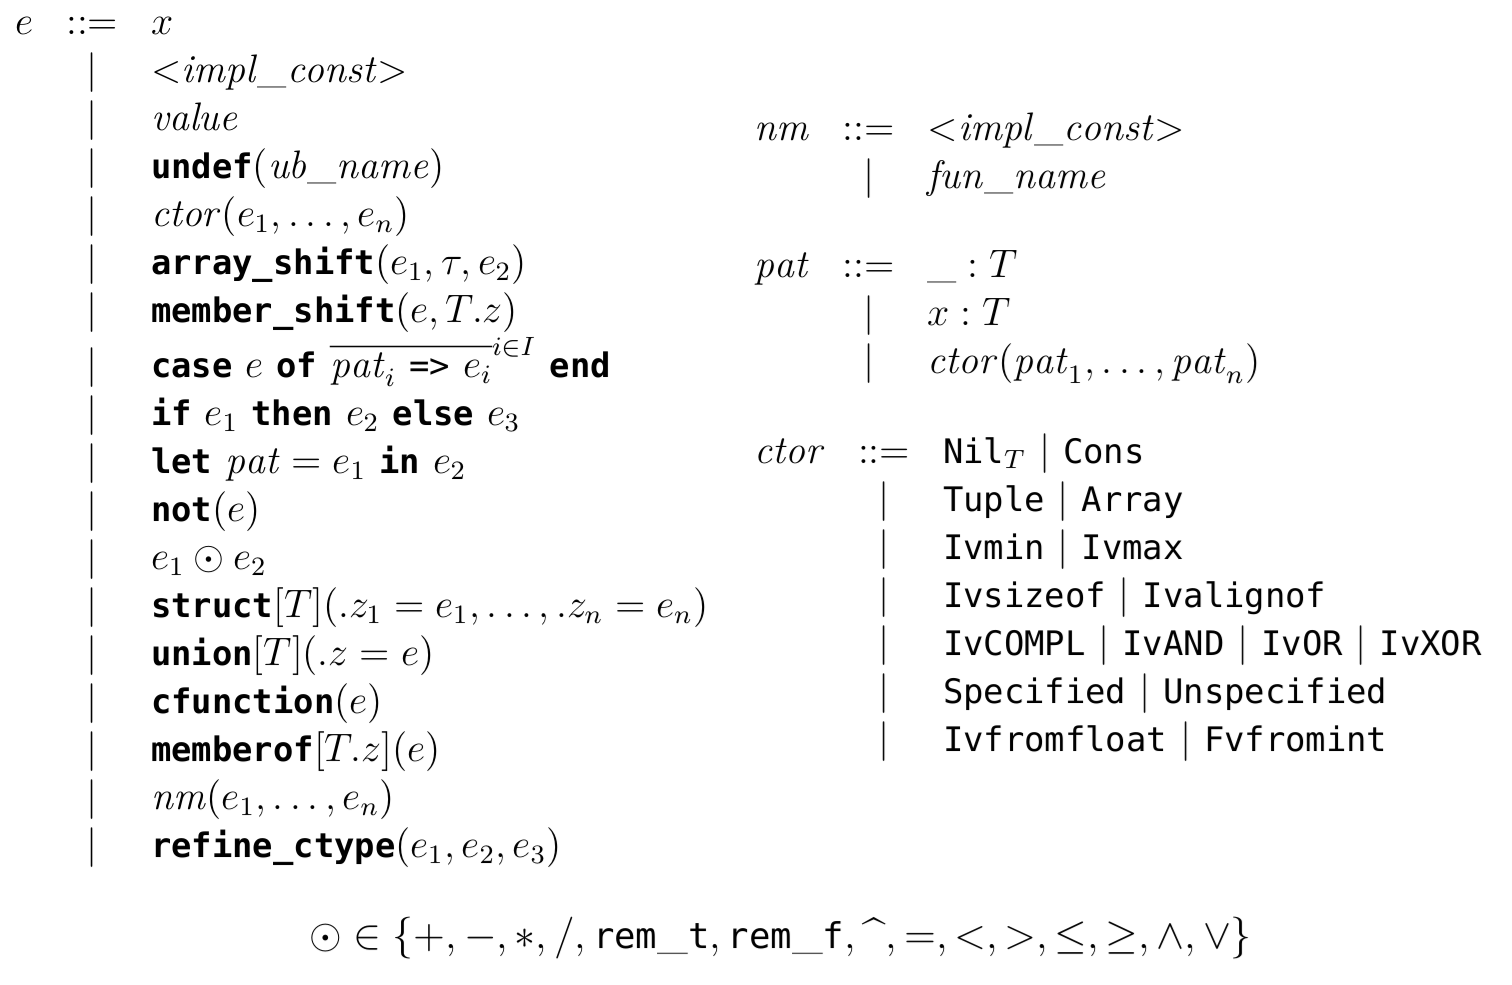
\includegraphics{figures/pure-core.png}
    \caption{The pure fragment of Core.}\label{fig:pure-core-grammar}
\end{figure*}

The effectful fragment captures interactions with memory (via a memory
interface), various ordering constraints, and more exotic control flow with a
goto-like operator used in the elaboration of C's iteration and \cinline{goto}
statements. The distinction between the pure and effectful fragments is is in
fact unrelated to the distinction between expressions and statements in C,
since both are elaborated into effectful expressions (for example,
\coreinline{PtrEq} which tests for for pointer equality).

I will discuss \coreinline{memop()} in more detail in % chktex 36
\nameref{chap:mem-model-explained}. For now it suffices to say that the
operations are effects, part of the memory interface \kl{Core} uses to abstract
over choices of different handlers, implementations of those effects in a
specific memory object model.

The following constructs are all related to evaluation order:
\coreinline{neg()}, \coreinline{unseq()}, \coreinline{let weak}, % chktex 36
\coreinline{let strong}, \coreinline{bound()}, \coreinline{nd()}, % chktex 36
\coreinline{par()}. These were supported in the implementation but  % chktex 36
stopped working due to a refactor of the resource inference scheme, and not
enough of a priority to re-enable. I did not attempt to formalise their
operational behaviour.\sidenote{The technique for doing so would simple
enough conceptually (using fractional-permissions), but capturing the allowable
behaviours in the type system accurately and threading it through the rest of
the formalisation would add unnecessary noise and complexity at this stage.}

The \coreinline{ccall()} and \coreinline{pcall()} constructs for calling % chktex 36
elaborate C functions and Core procedures (effectful functions) respectively.
They differ only in how the name of the procedure to be called is found, with
\coreinline{ccall()} using the memory interface to do so. % chktex 36

The \coreinline{save()} operator is \kl{Core}'s way of introducing named % chktex 36
continuations with default arguments. The label $l$ and arguments $x_1, \ldots,
x_n$ are in scope in $E$; those variables are associated pure expressions
provided by the \coreinline{run()} operator or with the default $e_1, \ldots, % chktex 36
e_n$ otherwise if the operator is reached otherwise. This is the \cinline{goto}-like
operator referred to earlier, which is used to elaborate all of C's iteration
and \cinline{goto} statements.

The important aspect from our purposes is that while control flows into
\coreinline{ccall()}, \coreinline{pcall()} and \coreinline{run()}, it % chktex 36
only returns from the first two and not the last.

\begin{figure*}[tp]
    \ContinuedFloat{}
    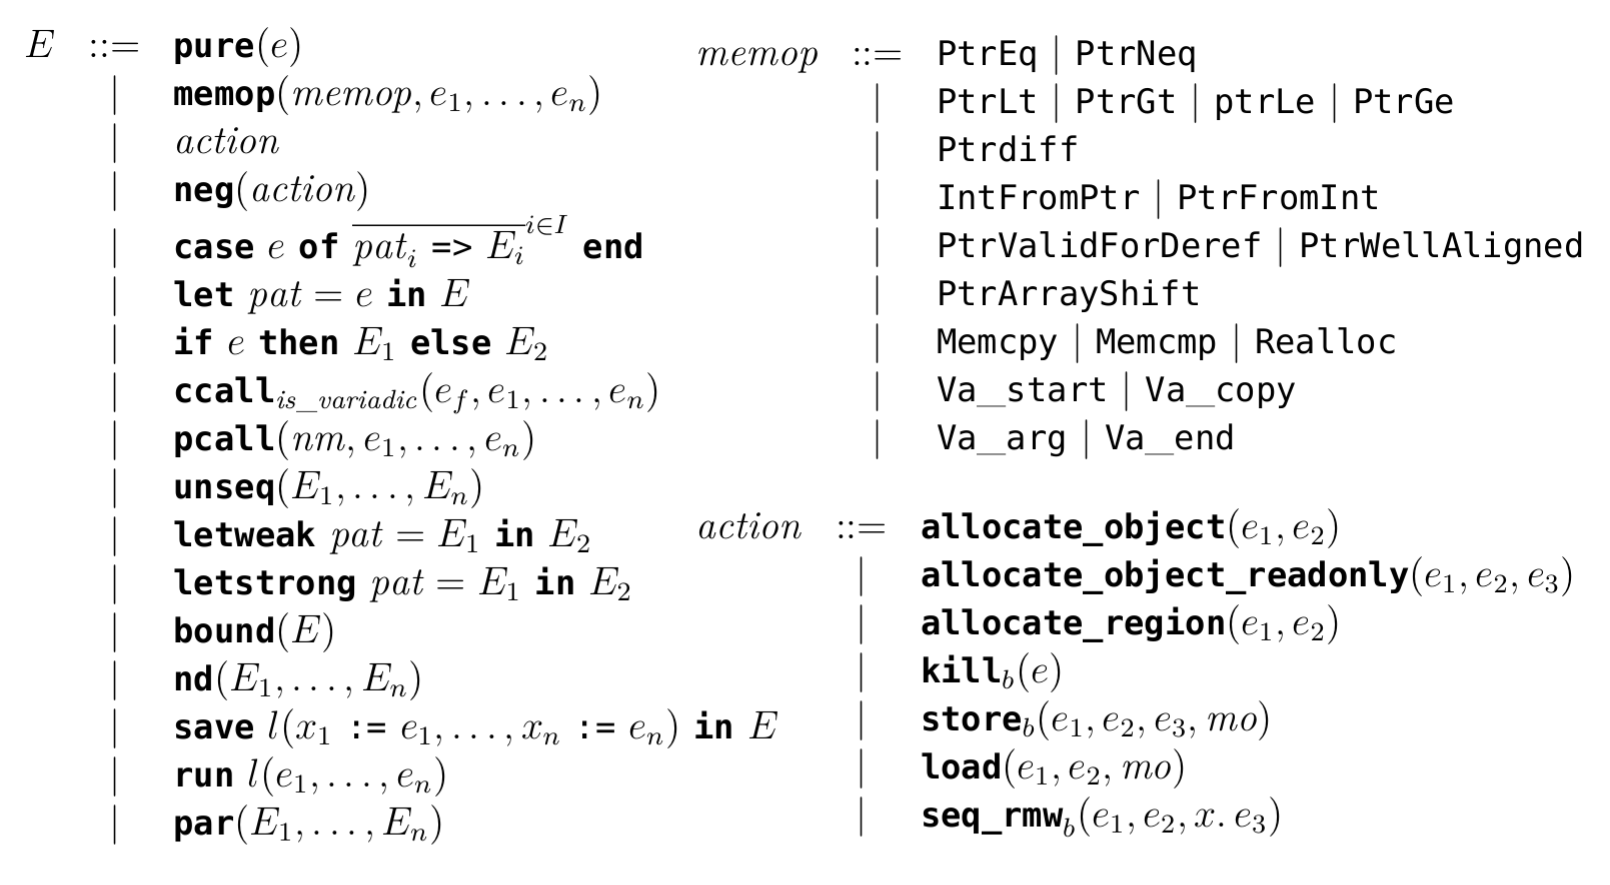
\includegraphics{figures/effectful-core.png}
    \caption{The effectful fragment of Core.}\label{fig:effectful-core-grammar}
\end{figure*}

We can see an example of Cerberus' elaboration into \kl{Core}, by recalling the
singly-linked integer list append function from \cref{fig:append-c}, reproduced
in \cref{fig:append-c-formal} for convenience.

\begin{marginfigure}
    \centering
    \cfile[breaklines]{code/append_plain.c}
    \caption{Singly-linked integer list append in C.}\label{fig:append-c-formal}
\end{marginfigure}%

\begin{figure*}[p]
    \centering
    \begin{minipage}{1.2\textwidth}
        \corefile{code/append_plain.core}
    \end{minipage}
    \caption{Elaboration of singly-linked int list append in C into
        \kl{Cerberus} \kl{Core}; library functions and \cinline{else}-branch
        omitted.}\label{fig:append-core}
\end{figure*}%

The elaboration is presented in \cref{fig:append-core}. To save space,
definitions the \kl{Core} standard library are omitted, as are choices about
implementation-defined details and the elaboration of the
\cinline{else}-branch. A few things are note-worthy:
\begin{itemize}
    \item The translation is \intro{compositional}. Each function, block,
        statement and expression is elaborated in isolation, based only
        on its parts, and follows the structure of the original C program.
    \item Each variable function argument and local gets its own storage via the
        \coreinline{create} function. Reads, writes, and de-allocations are
        represented with \coreinline{load}, \coreinline{store},
        \coreinline{kill} respectively.
    \item Loose evaluation order (for example between the expressions of a \cinline{==})
        are represented using \coreinline{unseq} and \coreinline{let weak} constructs.
    \item UB is made explicit in the syntax of the program, for example if \cinline{xs} was
        an unspecified pointer value (line 23) or if the function exited without a return statement
        and its `return value' was used elsewhere (line 71).
\end{itemize}

In particular, \kl{compositional}ity is just as important, if not more, than the
target language being a first-order functional language with effects. Given
that we want users to annotate programs at the C level, if we wish to type
check \kl{Core}, we need to be able to transport those annotations through the
elaboration process too, and place them at the appropriate program points.

If \kl{Cerberus} were to have elaborated into a dataflow graph instead of \kl{Core},
such transporting would be a major undertaking in itself. It might achievable
for function pre- and postconditions, but would become much more challenging
for loops, and \coreinline{goto} and even between specific statement as proof
hints to \kl{CN}. With a \kl{compositional} mapping, placing annotations
structurally, and relating annotations mentioning C variables to \kl{Core}
variables becomes feasible.

In principle, the compositional mapping also ensures that errors in \kl{Core}
elaboration can be related back to useful source locations in the original C
program. However, in practice, though \emph{compositional}ity does
\emph{enable} this, it requires a good amount of engineering effort to
accomplish (\cref{sec:error-msgs}). Another challenge is that though
elaboration simplifies greatly the checked language, it also increases the
distance between the checked and the typed language, which is felt acutely when
attempting to relate failures in SMT queries back to what users wrote,
particularly when those SMT are part of an inference procedure, rather checking
C source assertions (\cref{sec:counter-ex}).

\section{Refinement Types}

What are refinement types? Why do we care about decidability? It's a short hand
for usable, SMT, imperfect proxy for performance, to be discussed later.

You can layer over the existing system (from Kayvan's thesis), \textendash{}
rule for undef means (previously YOLO) to context has to be false. E\.g\. same if-then-else twice, so dead code.

Liquid types.

\section{Linearity}

\subsection{Friendly and convenient syntax}\label{sec:friendly-syntax}
Separation logic types, syntax and restrictions for it.

Explicit witness to having permissions, which are linearly typed (just ingredients).

\section{Alternatives and Related Work}

\chapter{Kernel CN:\ A Bidirectional, Separation Logic Refinement Type System for Core}%
\label{chap:kernel-cn}

This will be a lot of pages.
Explain \intro{bidirectional} (for quantifiers), linear resources, constraints.
Explain enough rules \textemdash{} typing, operations, especially the weird heaps.
And of course, type safety statement and its proof.

\subsection{Resource Terms, Quantifier Inference}

Linear terms in a refinement type system.

(Dep ML, L3, F star, Jhala, ATS)

Different and unusual compared to Iris style \textemdash{} separation proofs outside the program.

Proof term in one sense, but also factors out operations for resource manipulation.

\subsection{Heaps}


\subsection{Type Safety}


%TC:ignore
\chapter{Warm-up: CCω}
\label{chap:bidir-ccw}

\margintoc

% In this chapter, we give an alternate presentation of \kl{CCω}, as defined in
% \cref{fig:ccw-typing}. Most of the ideas are abstract over the notion of \kl{conversion}
% that is considered,
% so either \kl(conv){declarative} or \kl(conv){algorithmic} conversion can be used without
% much impact.

\section{Turning \kl(tit){CCω} Bidirectional}
\label{sec:bidir-ccw}

\subsection{McBride’s discipline}
\label{sec:bidir-mcbride}

\AP To design our bidirectional type system, we follow a discipline exposed by McBride
\sidecite[1em]{McBride2018,McBride2019}.
The central point is to distinguish in a judgement between three \intro{modes}:
the \reintro{subject},
whose well-formation is under examination, \reintro{inputs},
whose well-formation is a condition for the judgement to be meaningful,
and \reintro{outputs}, whose well-formation should be a consequence of the judgement.
By \intro{well-formed}, which we use indistinctly for contexts, terms and types,
we mean:
\begin{itemize}
  \item $\vdash \Gamma$ in the case of a context $\Gamma$,
  \item $\Gamma \vdash T \ty \uni$ in the case of a type $T$,
  \item the existence of some $T$ such that $\Gamma \vdash t \ty T$ in the case of a term $t$.
\end{itemize}
For the last two, this is relative to an implicit context $\Gamma$.
We also use \reintro{well-typed} for a term, with the same meaning as \kl{well-formed}.

\AP In the case of \intro{inference} $\intro*\inferty{\Gamma}{t}{T}$, the subject is $t$,
$\Gamma$ is an input and $T$ is an output.
On the contrary, in \intro{checking} $\intro*\checkty{\Gamma}{t}{T}$, $t$ is still the subject
and $\Gamma$ is an input, but this time $T$ is an input as well.
This means that one should consider whether $\inferty{\Gamma}{t}{T}$
only in cases where $\vdash \Gamma$ is already known,
and if the judgement is derivable it should be possible to conclude that
not only $t$, but also $T$ are well-formed.

In order to enforce this property globally, all inference rules should locally
preserve it as an invariant.%
\sidenote{The motto – slightly adapted from \textcite{McBride2018} – is:
  \textit{A rule is a server for its conclusion and a client for its premises.
  Servers receive promises about inputs and make promises about outputs, clients make
  promises about inputs and receive promises about outputs.}}
More precisely, information flows in a clockwise manner. First, we can assume that inputs
to the conclusion are well-formed, as inputs to the whole rule. Next, we move to the
premises. Here the constraint is reversed: we should ensure that inputs to a premise are
well-formed, but can assume that its outputs and subjects are. We might need to use
the well-formation of subjects or outputs of previous ones for that.
Finally, information goes to the conclusion again, and now not only the subject but also
the output should be well-formed if all those of the premises are.

\begin{figure*}
  \begin{mathpar}
  % \inferrule[(1)]
  %   {\phantom{\Gamma \vdash t \pity{\P} \P x : A. B}}
  %   {\Gamma \vdash \tikzmarkin{s1} t\ u \tikzmarkend{s1} \ity \phantom{\subs{B}{x}{u}}} \and
  \inferrule[(1)]
    {\tikzmarkin[ch]{p2}\Gamma \tikzmarkend{p2} \vdash
      \tikzmarkin[uc]{p23} t \pity{\P} \P x : A. B \tikzmarkend{p23}\\
      \tikzmarkin[ch]{p21}\Gamma\tikzmarkend{p21} \vdash
      \tikzmarkin[uc]{p22} u \cty A\tikzmarkend{p22}}
    {\tikzmarkin[ch]{c2}\Gamma\tikzmarkend{c2} \vdash
      \tikzmarkin[uc]{c21}t\ u \ity \subs{B}{x}{u}\tikzmarkend{c21}} \and
  \inferrule[(2)]
  {\tikzmarkin[ch]{p3}\Gamma \vdash t \pity{\P} \P x : A. B \tikzmarkend{p3}\\
    \tikzmarkin[ch]{p31}\Gamma\tikzmarkend{p31} \vdash
    \tikzmarkin[uc]{p32} u \cty A\tikzmarkend{p32}}
  {\tikzmarkin[ch]{c3}\Gamma\tikzmarkend{c3} \vdash
    \tikzmarkin[uc]{c31}t\ u \ity \subs{B}{x}{u}\tikzmarkend{c31}} \and
  \inferrule[(3)]
  {\tikzmarkin[ch]{p4}\Gamma \vdash t \pity{\P} \P x : A. B \tikzmarkend{p4}\\
    \tikzmarkin[ch]{p41}\Gamma\tikzmarkend{p41} \vdash
    \tikzmarkin[uc]{p42} u \tikzmarkend{p42} \cty \tikzmarkin[ch]{p43}A\tikzmarkend{p43}}
  {\tikzmarkin[ch]{c4}\Gamma\tikzmarkend{c4} \vdash
    \tikzmarkin[uc]{c41}t\ u \ity \subs{B}{x}{u}\tikzmarkend{c41}} \and
  \inferrule[(4)]
  {\tikzmarkin[ch]{p5}\Gamma \vdash t \pity{\P} \P x : A. B \tikzmarkend{p5}\\
    \tikzmarkin[ch]{p51}\Gamma \vdash u \cty A\tikzmarkend{p51}}
  {\tikzmarkin[ch]{c5}\Gamma\tikzmarkend{c5} \vdash
    \tikzmarkin[uc]{c51}t\ u \ity \subs{B}{x}{u}\tikzmarkend{c51}} \and
  \inferrule[(5)]
  {\tikzmarkin[ch]{p6}\Gamma \vdash t \pity{\P} \P x : A. B \tikzmarkend{p6}\\
    \tikzmarkin[ch]{p61}\Gamma \vdash u \cty A\tikzmarkend{p61}}
  {\tikzmarkin[ch]{c6}\Gamma \vdash t\ u \ity \subs{B}{x}{u}\tikzmarkend{c6}}
  \end{mathpar}
  \caption{An illustration of McBride’s discipline (well-formed objects are in blue, those not known to be so are in red)}
  \label{fig:bidir-mcbride}
\end{figure*}

As an illustration, an example of a rule that respects this discipline – that
for application – is given in \cref{fig:bidir-mcbride}.
Let us ignore for an instant the exact meaning of the judgement $\mathord{\pity{\P}}$
which we introduce soon, and whose modes are the same as inference.
Instead, focus on well-formation: objects known to be well-formed
are on a blue background, those which are not are on a red one.
First, $\Gamma$ is well-formed, as an input to the conclusion (1). Thus
we can thus move to the first premise, since its only input is $\Gamma$.
From that premise holding, we learn that $t$ and $\P x : A.\ B$ are well-formed (2).
Therefore, $A$ is in particular well-formed, and we can move to the second premise
whose two inputs are now known to be well-formed (3). From it, we learn
that $u$ is well-formed (4). Now we can deduce that $t\ u$ is well-formed. But this is
not enough: since $\subs{B}{x}{u}$ is an output of the conclusion,
we must ensure it is well-formed too. Fortunately,
it is, since $\P x : A.\ B$ is, so $B$ is too,%
\sidenote{In the extended context $\Gamma, x : A$.}
and so $\subs{B}{x}{u}$ is as well, since $\Gamma \vdash u \cty A$.
Thus, we can move back to the conclusion (5), which ends our roundtrip.

A somewhat similar discipline has appeared independently in
\sidetextcite[][Section 4]{Dunfield2021}, where it is called ”Pfenning’s recipe”.
The main criterion is \emph{mode-correctness}, which demands
an information flow similar to McBride’s, but is coarser, as it does not
consider well-formation of the objects, only their knowledge. For instance,
in the case of $\l x : A.\ t$, that criterion allows to directly extend a context
with $A$ to infer a type for $t$, because it is known,
but McBride’s discipline forbids it, because $A$’s well-formation is not established.
Another related condition is also used in \sidetextcite{Bauer2020}.
The authors introduce the notions of a \emph{(weakly) presuppositive type theory}
\cite[Def.~5.6]{Bauer2020} and of \emph{well-presented} premise-family and rule-boundary
\cite[Def.~6.16 and 6.17]{Bauer2020}, using what they call the \intro{boundary} of a judgement
as the analogue of our \kl{inputs} and \kl{outputs}.
Due to their setting being undirected, this is however more restrictive,
because they are not able to distinguish inputs from outputs and thus cannot relax the
condition to only demand inputs to be well-formed but not outputs.

\AP Because of our dependently typed setting, we actually need to introduce a third judgement,
beyond the already mentioned \kl{inference} and \kl{checking}:
\intro{constrained inference}, written
$\intro*\pinferty{h}{\Gamma}{t}{T}$, where $h$ is either $\Pi$ or $\uni$.%
\sidenote{These are the only type formers in \kl{CCω}, but
in \kl{PCUIC}, $h$ can also be \eg an inductive type.}
Constrained inference is a judgement%
\sidenote{Or, rather, a family of judgements indexed by $h$.}
with the exact same \kl{modes} as \kl{inference},
but where the type output is not completely free.
Rather, as the name suggests, a constraint is imposed on it, namely that its head constructor can only be the corresponding element of $h$.
This is needed to handle the behaviour absent in simple types that some terms might not have a desired type “on the nose”. Take for instance the first premise
$\Gamma \vdash t \ty \P x : A .\ B$ of \ruleref{rule:cic-app}.
What bidirectional judgement should replace it?
It would be too much to ask $t$ to directly infer a Π-type, as some reduction might be needed to uncover this $\P$. Checking also cannot be used, because the domain and codomain of the tentative Π-type are not known at that point: they should be inferred from $t$.

Finally, this mode distinction also applies to computation-related judgements,
although those have no subject.
Instead, what is under scrutiny is the “computational content” of the rule.
For conversion $\Gamma \vdash T \conv T' : \uni$, 
both $T$ and $T'$ are inputs and thus should be known to be well-formed beforehand.
For reduction $T \red T'$, on the contrary, $T$ is an input,
but $T'$ is an output. Hence, only $T$ needs to be well-formed \textit{a priori},
and we rely on the \kl{subject reduction} property to ensure
that the output $T'$ also is.

\subsection{The typing rules}

To transform the rules of \kl{CCω} as given in \cref{fig:ccw-typing}, 
start by recalling that we wish to obtain a complete bidirectional type system.
Therefore, any term should infer a type, and thus
all rules where the subject of the conclusion starts with a term former
should give rise to a rule with \kl{inference} as a conclusion.
It thus remains to choose the judgements for the premises,
which amounts to determining their \kl{modes}.
If a term in a premise appears as input in the conclusion or output of a previous premise, then it can be considered an input, otherwise it must be an output. Moreover, if a type output is unconstrained, then \kl{inference} can be used, otherwise we must resort to
\kl{constrained inference}. This transformation leads to the rules of \cref{fig:ccw-bidir-infer}.

\begin{figure}[ht]
  \ContinuedFloat*
  \begin{mathpar}
    \inferdef{Var}
      {(x : T) \in \Gamma}
      {\inferty{\Gamma}{x}{T}}
    \label{rule:bd-var} \and
    \inferdef{Univ}
      { }
      {\inferty{\Gamma}{\uni[i]}{\uni[i+1]}}
    \label{rule:bd-univ} \and
    \inferdef{ΠTy}
      {\pinferty{\uni}{\Gamma}{A}{\uni[i]} \\
        \pinferty{\uni}{\Gamma, x : A}{B}{\uni[j]}}
      {\inferty{\Gamma}{\P x : A .\ B}{\uni[\umax{i}{j}]}}
    \label{rule:bd-prod} \and 
    \inferdef{Abs}
      {\pinferty{\uni}{\Gamma}{A}{\uni[i]} \\ \inferty{\Gamma, x : A}{t}{B}}
      {\inferty{\Gamma}{\l x : A .\ t}{\P x : A .\ B}}
    \label{rule:bd-abs} \and
    \inferdef{App}
      {\pinferty{\Pi}{\Gamma}{t}{\P x : A .\ B} \\ \checkty{\Gamma}{u}{A}}
      {\inferty{\Gamma}{t\ u}{\subs{B}{x}{u}}}
    \label{rule:bd-app} \\
  \end{mathpar}
  \caption{Rules for inference in bidirectional \kl{CCω}}
  \label{fig:ccw-bidir-infer}
\end{figure}

In anticipation, we set the typing rules for \kl{CCω} so that this transformation would be
direct. This particularly applies to the undirected \ruleref{rule:cic-abs},
recalled opposite.
Indeed, there are at least two other ways to write it, which do not lead to a valid
bidirectional presentation.
\marginnote{
  \normalsize
  \begin{mathpar}
  \inferrule*[vcenter,right=Abs]
  {\Gamma \vdash A \ty \uni \\ \Gamma, x : A \vdash t \ty B}
  {\Gamma \vdash \l x : A.\ t \ty \P x : A.\ B}
  \end{mathpar}
}
The first, which is the usual one in \kl{Pure Type Systems} (\kl{PTS})
\sidecite{Barendregt1991},
is to have $\Gamma \vdash \P x : A.\ B \ty \uni$ as a premise
instead of $\Gamma \vdash A \ty \uni$. In the setting of a general \kl{PTS},
this is needed, because not every Π-type is well-formed,
even if the domain and codomain are.%
\sidenote{\kl{PTS} where this is true are called \intro{full}.}
However, this premise is problematic in the bidirectional setting. Indeed, $B$ can only be
inferred as a type for the body of the abstraction $t$. But to infer a type for $t$, the
context $\Gamma, x : A$ needs to be well-formed, which is not known if this premise is
the first one.
This issue has been identified by \sidetextcite{Pollack1992}, who remarked that the
bidirectional structure we present here is only equivalent to the undirected one
in semi-full \kl{PTS} – a slight generalization of the full ones.
In a full \kl{PTS}, the opposite path of simply removing the first premise altogether
can also be taken, relying on \kl{validity} to ensure that $\vdash \Gamma, x \ty A$ and thus
$\Gamma \vdash A : \uni$. But again, in a bidirectional setting,
this does not respect McBride’s discipline.

The main difference between the bidirectional and undirected rules is that we dropped
hypotheses of context well-formation in Rules~\nameref{rule:bd-univ} and
\nameref{rule:bd-var}. Indeed, since the context is always supposed to be well-formed
as an input to the conclusion, it is not useful to re-check it. This is also in line with implementations, where the context is not checked at leaves of a derivation tree, with performance issues in mind. The well-formation invariants then ensure that any derivation starting with the (well-formed) empty context will only ever encounter well-formed contexts.

With the rules for term formers taken care of,
we are left with the single \ruleref{rule:cic-conv}.
\begin{marginfigure}
  \ContinuedFloat
  \begin{mathpar}
    \inferdef{Check}
      {\inferty{\Gamma}{t}{T'} \\ T' \conv T}
      {\checkty{\Gamma}{t}{T}}
    \label{rule:bd-check} \and
    \inferdef{UnivInf}
      {\inferty{\Gamma}{t}{T} \\ T \fred \uni[i]}
      {\pinferty{\uni}{\Gamma}{t}{\uni[i]}}
      \label{rule:bd-pinf-univ} \and
    \inferdef{ΠInf}
      {\inferty{\Gamma}{t}{T} \\ T \fred \P x : A. B}
      {\pinferty{\P}{\Gamma}{t}{\P x : A . B}}
      \label{rule:bd-pinf-prod}
  \end{mathpar}
  \caption{Computation rules for bidirectional \kl{CCω}}
  \label{fig:bidir-ccw-other}
  \end{marginfigure}
There are two different possible adaptations of this rule, depending on
\kl{modes} for computation.
In the case of \kl{checking}, the target type is an input, so
it can be compared to the inferred one using \kl{conversion}.
But in the case of \kl{constrained inference} it is unknown, and so
we must resort to \kl{reduction} to obtain it from the inferred one.
Using \kl{conversion} would not respect modes, since it has two inputs.
This eventually leads to the decomposition of \ruleref{rule:cic-conv} into
\ruleref{rule:bd-check} in the first case, while
\nameref{rule:bd-pinf-univ} and \nameref{rule:bd-pinf-prod} correspond to the second case.
Note that while the way conversion and reduction can be used in derivations have changed,
those relations themselves remain untouched,
we only refined them by giving them an explicit mode.
We also do not need to choose one or the other notion of \kl{conversion} yet. Instead, we can
stay abstract, only listing the properties we need from it in order to establish the
equivalence.

\subsection{Constrained inference in disguise}

This need to split the conversion rule into a reduction and conversion sub-routines depending on the mode is of course known to the implementors of proof assistants \sidecite{Abel2011}.
It explains in part the ubiquity of \kl(red){weak-head} reduction
in the dependently typed setting.
Indeed, it is exactly the minimal reduction strategy that is needed to expose the
head constructor of a type, and thus to implement constrained inference.

Still, reduction is only a means to determine whether a certain term fits into
a certain kind of types. In the setting of \kl{CCω}, this is basically the only way to do.
However, as soon as conversion is extended or modified,
% for instance with unification
% \sidecite{Asperti2012}, coercions \sidecite{Asperti2012,Sozeau2007}
% or graduality \sidecite{LennonBertrand2022},
reduction is often not enough any more.
Putting constrained inference forward explains some ideas that recurrently appear in
such settings:  they are not ad-hoc workarounds,
but are based on the need to account for constrained inference.

We already mentioned \sidetextcite{Pollack1992}, where $\Gamma \vdash t \ty T$ is used
for inference, and a judgement written $\Gamma \vdash t \mathrel{:\geq} T$ –
denoting type inference followed by reduction –
is used to effectively inline the two hypothesis of our constrained inference rules.
Checking is also inlined.
Similarly, \sidetextcite{Abel2008} use a judgement written $\Delta \vdash V \delta \Uparrow \operatorname{Set} \rightsquigarrow i$, where a type $V$ is checked to be well-formed, but with its exact level $i$ free. This corresponds very closely to our use of $\pity{\uni}$.
\sidetextcite{Gratzer2019} similarly use a judgement $\Xi \vdash T \Leftarrow type$,
but they do not bother inferring the level as they never have any need for it.

But the main area where constrained inference repeatedly becomes apparent is that of
elaboration. For instance,
\sidetextcite{Saibi1997} describes an elaboration mechanism inserting coercions between types.
This happens primarily during checking, when both types are known.
However, \citeauthor{Saibi1997} introduces two special classes to handle the need
to cast a term to a sort or a function type without more information,
exactly in the places where we resort to constrained inference instead of checking.
More recently, \sidetextcite{Sozeau2007} describes a system where conversion is augmented
to handle subset types.
As in \textcite{Pollack1992}, $\Gamma \vdash t \ty T$ is used for inference,
and the other judgements are inlined.
Once again, reduction is not enough to perform constrained inference, this time
because type constructors can be hidden in subsets:
an inhabitant of a type such as $\{f : \Nat \to \Nat \mid f\ \z = \z \}$
should be usable as a function of type $\Nat \to \Nat$.
An erasure procedure is therefore required on top of reduction to remove subsets in the places where we use constrained inference.

Analogous ideas can also be found in \kl{Matita}'s elaboration algorithm, as described in 
\sidetextcite{Asperti2012}.
Indeed, the presence of unification meta-variables on top of coercions makes it
even clearer that a specific treatment of what we identified as constrained inference is
required.
In the case of $\pity{\P}$, they have two rules to apply a function,
one where its inferred type reduces to a Π-type, corresponding to \ruleref{rule:bd-pinf-prod},
and another one to handle the case when the inferred type instead reduces to a meta-variable.
As \citeauthor{Saibi1997} and \citeauthor{Sozeau2007}, they also
need to handle coercions for terms in function position. However, their solution is different:
they introduce new meta-variables for the domain and codomain,
and rely on unification, which is available in their setting, to find values for those.
They also need to introduce a special judgement they call
\intro{type-level enforcing}, which corresponds to our $\pity{\uni}$ judgement.
The solution they take for Π-types is not viable there, as one would need a kind of universe
meta-variable. Instead, they rely on backtracking to test multiple possible universe choices.

Finally, in \arefpart{gradual}, somewhat akin to the use of meta-variables in
\textcite{Asperti2012}, there are two rules per constrained inference judgement.
One when the head constructor is the desired one – as for \kl{CCω} –,
and a second one to handle the wildcard $\?$, characteristic of gradual type systems.


\section{Properties of the Bidirectional System}
\label{sec:bidir-prop}

Let us now state and sketch proofs of the main properties of the bidirectional system.
The first two relate it to the
undirected one: it is both \kl(bidir){sound} – terms typeable in the bidirectional system are typeable in the undirected system – and \kl(bidir){complete} – all terms typeable in the undirected system are also typeable in the bidirectional system.
Next, we investigate \kl{uniqueness of types}, and its relation to the choice of a strategy for reduction.
Finally, we expose how \kl{strengthening} can be shown for undirected \kl{CCω}
by proving it on the bidirectional side.

\subsection{Soundness}

A bidirectional derivation can be seen as a refinement of an undirected derivation.
Indeed, the bidirectional structure can be erased to obtain an undirected derivation, 
replacing each bidirectional rule with the corresponding undirected rule.
As bidirectional rules lack some premises of the undirected ones, missing some sub-derivations
must be retrieved by relying on the well-formation invariants going with McBride’s discipline.
Thus, we get the following soundness theorem – note how the
discipline manifests as well-formation hypothesis on inputs.

\begin{minipage}{\textwidth}
\begin{theorem}[\intro{Soundness} of bidirectional typing for \kl{CCω}]
  \label{thm:corr-ccomega}
  If $\Gamma$ is well-formed and $\inferty{\Gamma}{t}{T}$ or $\pinferty{h}{\Gamma}{t}{T}$,
  then $\Gamma \vdash t \ty T$.
  If both $\Gamma$ and $T$ are well-formed and
  $\checkty{\Gamma}{t}{T}$, then $\Gamma \vdash t \ty T$. 
\end{theorem}  
\end{minipage}

  
\begin{minipage}{\textwidth}
\begin{proof}
  By mutual induction on the bidirectional typing derivation.

  Each rule of the bidirectional system can be replaced by the corresponding rule of the
  undirected system, with all three rules \nameref{rule:bd-check}, \nameref{rule:bd-pinf-univ} and \nameref{rule:bd-pinf-prod} replaced by
  \nameref{rule:cic-conv}. In all cases, the induction hypothesis can be used on sub-derivations of the bidirectional judgement, because context extensions and checking are
  done with types that are known to be well-formed,%
  \sidenote{This is the point where following McBride’s discipline is crucial!}
  by induction hypothesis on previous premises and possibly \kl{validity}.

  Some sub-derivations of the undirected rules that have no counterpart
  in the bidirectional ones are however missing.
  In Rules \nameref{rule:cic-univ} and \nameref{rule:cic-var},
  the hypothesis that $\Gamma$ is well-formed is enough to get the required premise.
  For \ruleref{rule:bd-check},
  the well-formation hypothesis on the type is needed to get the typing premise of
  \nameref{rule:cic-conv-unty}.
  As for Rules \nameref{rule:bd-pinf-univ} and \nameref{rule:bd-pinf-prod},
  that typing premise is obtained by combining the induction hypothesis,
  validity and \kl{subject reduction}.

  Alternatively, the appeal to validity could be removed by
  strengthening the theorem to incorporate the well-formation of outputs on top of that of
  the subject. Here we follow the proofs in \kl{MetaCoq}, which establishes
  meta-theoretical properties of the undirected system first – including validity –,
  so we can exploit these.
\end{proof}
\end{minipage}

\subsection{Completeness}

Contrarily to soundness, which keeps the structure of a derivation,
completeness is of a different nature.
Because in bidirectional derivations the computation rules are much less liberal than in
undirected ones, the structure of derivations must be altered.
The crux of the proof is thus to ensure that all uses of \ruleref{rule:cic-conv}
can be permuted down through the other rules,
in order to concentrate them in the places where they are authorized in the bidirectional
derivation.
In a way, composing completeness with soundness gives a kind of normalization procedure
on undirected derivations, which produces a canonical one by pushing conversion
down as much as possible.

The proof mainly relies on the following lemma,
which can be seen as a strong form of \kl{injectivity of type constructors} – 
the version of \cref{prop:prod-inj} is a direct consequence.

\begin{lemma}[Conversion implies reduction for type constructors]
  \label{lem:conv-red-tycons}
  If $T \conv \uni[i]$, then $T \red \uni[i]$.

  If $T \conv \P x : A.\ B$, then there exist $A'$ and $B'$ such that:
  \begin{itemize}
    \item $T \red \P x : A'.\ B'$
    \item $A' \conv A$
    \item $B' \conv B$
  \end{itemize}
\end{lemma}

\begin{minipage}{\textwidth}
\begin{proof}
  Let us spell out the proof on Π-types – the case of $\uni$ is similar, but easier.

  For \kl{algorithmic conversion}, by definition there must exist $T'$ and $T''$
  such that $T \red T'$, $\P x : A.\ B \red T''$, $T' \alpheq T''$.
  But there can be no \kl(red){top-level} reduction step in $\P x : A.\ B \red T''$,
  so actually $T''$ is some $\P x : A''.\ B''$ and $A \red A''$, $B \red B''$.
  Similarly, $T'$ must be some $\P x : A'.\ B'$
  such that $A' \alpheq A''$ and $B' \alpheq B''$.
  Combining these, we obtain that $A' \conv A$ and $B' \conv B$, as expected.

  For \kl{declarative conversion}, we can go through the
  equivalence with algorithmic conversion – and thus use \kl{confluence} under
  the hood.
\end{proof}  
\end{minipage}


\begin{theorem}[\intro{Completeness} of bidirectional typing for \kl{CCω}]
  \label{thm:compl-ccomega}
  If $\Gamma \vdash t \ty T$, then there exists $T'$ such that $\inferty{\Gamma}{t}{T'}$
  and $T' \conv T$.
\end{theorem}

\begin{proof}
  By induction on the undirected typing derivation.
  
  Rules \nameref{rule:cic-var} and \nameref{rule:cic-univ} are base cases,
  and can be simply replaced by the corresponding bidirectional rules.
  In the case of \ruleref{rule:cic-conv}, the property is a direct consequence of the induction hypothesis, together with transitivity of conversion:
  we simply conflate two conversions together.
  
  As for \ruleref{rule:cic-prod}, the induction hypothesis on the domain $A$
  gives the existence of $T_A$
  such that $\inferty{\Gamma}{A}{T_A}$ and $T_A \conv \uni[i]$. Using
  \cref{lem:conv-red-tycons}, we can derive $\pinferty{\uni}{\Gamma}{A}{\uni[i]}$.
  Applying a similar reasoning on the codomain and combining both is enough to conclude.

  In \ruleref{rule:cic-abs}, we do the same reasoning again on the type annotation.
  Combined with the induction hypothesis on the body $t$,
  we get $\inferty{\Gamma}{\l x : A.\ t}{\P x : A .\ B'}$ for some $B'$ such that $B \conv B'$, and thus $\P x : A . B \conv \P x : A . B'$ as desired.

  We are finally left with \ruleref{rule:cic-app}.
  Again, the key is \cref{lem:conv-red-tycons}, which can be combined with the induction
  hypothesis on the function $f$ to get $\pinferty{\P}{\Gamma}{f}{\P x : A' .\ B'}$
  for some $A'$ and $B'$ such that $A \conv A'$ and $B \conv B'$,
  where $\P x : A. B$ is the type of $f$ in the undirected derivation.
  The induction hypothesis on the argument $u$ gives
  $\inferty{\Gamma}{u}{A''}$ with $A'' \conv A$. Thus, by transitivity of conversion
  $\checkty{\Gamma}{u}{A'}$, and we can apply \ruleref{rule:bd-app} to conclude.
\end{proof}

Interestingly, the proof of soundness relies on \kl{subject reduction}, which itself
needs \kl{injectivity of type constructors} and transitivity of conversion.
Similarly, completeness relies both on the injectivity as given by \cref{lem:conv-red-tycons},
and transitivity of conversion. Be it for algorithmic or declarative conversion, one at
least of those is not directly provable – we need \kl{confluence}.
We already hit this same tension between injectivity and transitivity 
with \kl{subject reduction}, and
must draw the same conclusion: there is no free lunch!

\Cref{thm:compl-ccomega} is quite specific to our \kl{Church-style} design.
Instead, an important portion of the research on bidirectional typing in the context
of dependent types adopts a \kl{Curry-style} approach.
This is the case of \eg \sidetextcite{Coquand1996}, the type system of \kl{Agda} as described
by \sidetextcite{Norell2007}, and most of the work by Abel
\sidecite{Abel2007,Abel2008,Abel2011,Abel2017},
and McBride \sidecite{McBride2016,McBride2018,McBride2019}.
In such systems, λ-abstractions can only be checked against a given type, but cannot infer one,
which implies that only terms with no redexes are typeable.
\textcite{Norell2007} argues that explicit
redexes are uncommon in real-life programs, so that being unable to type them is not a strong
limitation in practice. Another solution, taken by \textcite{McBride2022}, is to add
type annotations in order regain the ability to check non-normal terms,
at the cost of inserting annotations at the right place.
In all cases, however, the fact that all terms well-typed in the declarative system infer
a type is irremediably lost. Weaker forms of completeness should still hold for such systems,
typically one where all terms check against their type, but are not ensured to infer.
See for instance \sidetextcite[][Theorem~7.3]{Gratzer2019} for one restricted to normal forms
– and thus not taking the role of annotations into account.

\begin{marginfigure}
  \begin{mathpar} 
    \inferrule
    {T \hred \P x : A' . B \\ \pinferty{\uni}{\Gamma}{A}{\uni[i]} \\
    A \conv A' \\ \checkty{\Gamma, x : A}{t}{B}}
    {\checkty{\Gamma}{\l x : A.\ t}{T}}
  \end{mathpar}  
\end{marginfigure}

In a setting with \kl{Church-style} abstraction,
if one wishes to give the possibility for seemingly untyped abstraction,
another mechanism has to be resorted to, typically elaboration using meta-variables.
This is described in \eg \textcite{Asperti2012},
which combines a rule similar to \ruleref{rule:bd-abs}
– where the type of an abstraction is inferred – with another one,
similar to the \kl{Curry-style} one – where abstraction is checked, see opposite.
While such a rule would make a system as that we have just described “over-complete”,
it is a useful addition to enable the propagation of checking information
upwards in the derivation, which is crucial in elaboration phases, even in \kl{Church-style}.

\subsection{Uniqueness}

All the bidirectional judgements of \cref{fig:ccw-bidir-infer} are syntax-directed,
in the sense that there is always at most one rule that applies to derive a certain typing judgement, given a fixed \kl{subject}.
But there is still some indeterminacy.
Indeed, in rules involving reduction no strategy is fixed, thus two different reducts can be used with the same rule, resulting in different inferred types.
However, inferred types are still related:

\begin{theorem}[Uniqueness of inferred type up to joinability]
  \label{thm:unique-inf}
  If $\Gamma$ is well-formed,
  $\inferty{\Gamma}{t}{T}$ and $\inferty{\Gamma}{t}{T'}$ then $T$ and $T'$ both reduce to a
  common $T''$, \eg $T \red T''$ and $T \red T''$.
  In particular, $T \conv T'$.
\end{theorem}

\begin{proof}
  By mutual induction on the first derivation, together with the same property for
  constrained inference.

  The main idea is to use \kl{confluence} to relate different reduction paths in Rules
  \nameref{rule:bd-pinf-prod} and \nameref{rule:bd-pinf-univ}. For the other rules,
  the conclusion is direct from the induction hypotheses.
\end{proof}

Combining this with \kl(bidir){soundness} and \kl(bidir){completeness},
we get \kl{uniqueness of types} for the undirected system.

\begin{theorem}[Uniqueness of types]
  \label{thm:unique-undir}
  If $\Gamma \vdash t \ty T$ and $\Gamma \vdash t \ty S$ then $T \conv S$.
\end{theorem}

\begin{minipage}{\textwidth}
\begin{proof}
  Since $\Gamma \vdash t \ty T$, by soundness
  there exists some $T'$ such that $\inferty{\Gamma}{t}{T'}$ and moreover $T' \conv T$.
  Similarly, there exists some $S'$ such that $\inferty{\Gamma}{t}{S'}$
  and moreover $S' \conv S$.
  But by uniqueness $T' \conv S'$, and thus $T \conv S$.
\end{proof}  
\end{minipage}


\begin{marginfigure}
\begin{mathpar}
  \inferdef{UnivWhInf}
    {\inferty{\Gamma}{t}{T} \\ T \hred \uni[i]}
    {\pinferty{\uni}{\Gamma}{t}{\uni[i]}}
    \label{rule:bd-pinf-wh-univ} \and
  \inferdef{ΠWhInf}
    {\inferty{\Gamma}{t}{T} \\ T \hred \P x : A. B}
    {\pinferty{\P}{\Gamma}{t}{\P x : A . B}}
    \label{rule:bd-pinf-wh-prod}
\end{mathpar}
\caption{Constrained inference with a weak-head strategy}
\label{fig:wh-pinf}
\end{marginfigure}

In order to completely eliminate indeterminacy, a reduction strategy can be fixed.
This amounts to replacing \kl{full reduction} with \kl{weak-head reduction},
\eg to replace the two reduction rules in \cref{fig:bidir-ccw-other} by those of
\cref{fig:wh-pinf}.
This is still \kl(bidir){sound} and \kl(bidir){complete}.
Soundness follows exactly the same proof as
\cref{thm:corr-ccomega}. As for completeness, the main point is to show an analogous
to \cref{lem:conv-red-tycons} for weak-head reduction.
  
\begin{theorem}[Reduction strategy]
  \label{thm:red-strat}

  If Rules \nameref{rule:bd-pinf-univ} and \nameref{rule:bd-pinf-prod} are replaced by
  \nameref{rule:bd-pinf-wh-univ} and \nameref{rule:bd-pinf-wh-prod},
  then given a well-formed context $\Gamma$ and a term $t$ there is at most one $T$
  such that $\inferty{\Gamma}{t}{T}$, and at most one $T'$ such that
  $\pinferty{h}{\Gamma}{t}{T'}$.
\end{theorem}

\begin{proof}
  Once again, by mutual induction.

  For inference, given a fixed term $t$ there is always at most one rule which applies to
  derive $\inferty{\Gamma}{t}{T}$, since there is exactly one rule per term former.
  Combining this with the uniqueness of types inferred in the premises by induction
  hypothesis is enough to conclude.

  For the constrained inference judgement, once again there is only one rule that applies.
  Since weak-head reduction is deterministic – given $T$, there is at most one $T'$ such that
  $T \hored T'$ –, there is at most one weak-head normal form $\uni$ or $\P x : A.\ B$ for
  a type. Hence, the type obtained by constrained inference is unique.
\end{proof}

\subsection{Strengthening}

Reasoning on the bidirectional derivation makes proofs easier,
while \kl(bidir){soundness} and \kl(bidir){completeness} ensure the results
can be carried to the undirected system.
One way to understand this is that the canonical derivation obtained by combining
soundness and completeness is more structured, and thus more amenable to proofs.

An example of this is the \kl{strengthening} property, a consequence of
\kl{conditional stability under renaming}. We explained in \cref{sec:tech-properties}
why proving these in the undirected system is not straightforward: the issue is that 
computation is too unconstrained, so that derivations might make use of needless variables.
Bidirectional typing, however, does not have this defect, since no type is ever "invented".
Rather, they are obtained either by reduction of previously inferred types, or as inputs.
This means that types in a bidirectional derivation never mention useless variables, and thus
that the following holds.

\begin{minipage}{\textwidth}
\begin{theorem}[Conditional stability under renaming – bidirectional]
  \label{thm:strong-stab-renaming-bidir}
  Whenever we have 
  \begin{itemize}
    \item $\inferty{x_1 : A_1 \dots x_n : A_n}{t}{T}$
    \item for all $i$ such that $x_i$ appears in $t$,
      there is a variable $y_i$ such that $(y_i : \multisubs{A_i}{x_1 \into y_1 \dots x_n \into y_n}) \in \Delta$
  \end{itemize} 
  it also holds that $\inferty{\Delta}{\multisubs{t}{x_1 \into y_1 \dots x_n \into y_n}}{\multisubs{T}{x_1 \into y_1 \dots x_n \into y_n}}$.
\end{theorem}
\end{minipage}

\begin{proof}
  By a direct induction on the typing derivation.

  Note that we do not even need $\Delta$ to be well-formed.
\end{proof}

And as a special case, \kl{strengthening} follows.

\begin{theorem}[Strengthening – bidirectional]
  \label{thm:strengthening-bidir}
  Whenever $\inferty{\Gamma, x : A}{t}{T}$ and $x$ does not appear in $t$,
  $\inferty{\Gamma}{t}{T}$ is derivable.
\end{theorem}

From those, \kl{conditional stability under renaming} and \kl{strengthening} for
the undirected system can be obtained without any difficulty.
\chapter{Bidirectional \kl(tit){PCUIC}}
\label{chap:bidir-pcuic}

\margintoc

As we have seen in \cref{sec:tech-pcuic}, there is much more to the real \kl{Coq} than
\kl{CCω}.
The ideas exposed in the previous chapter nevertheless
scale very well to these extensions.
There are two areas, though, where some care needs to be taken.
The first is cumulativity, which in particular forces us to reconsider the statement
of the completeness and uniqueness properties, see \cref{sec:bidir-pcuic-cumulativity}.
But the main one is the introduction of inductive types. In particular, there is a subtle
interplay with cumulativity in the treatment of pattern-matching.
Working on the formalized proof of completeness in \kl{MetaCoq} led to the discovery of
an incompleteness bug in the kernel of \kl{Coq} linked to this.
In \cref{sec:bidir-pcuic-inductives} we show how the bidirectional setting adapts to
inductive types, and try and give an intuition of the origin of the completeness issue.

We do not give precise proofs in this chapter,
instead relying on the formalization in \kl{MetaCoq} described in \arefpart{metacoq}.

  % The first area of difference are the universes. While on paper those are simply integer, to handle typical ambiguity and polymorphic (co)-inductive types, PCUIC uses algebraic universes, containing level variables, algebraic $\vee$ and $+1$ operators, and a special level for the sort Prop. Moreover, those universes are cumulative, that is they behave as if smaller universes were included in larger ones. The precise handling of the algebraic universes is abstracted away in MetaCoq, and quite similar in the directed and undirected systems, so it did not prove too difficult to handle. Cumulativity, however, introduces some not-so-small differences with the previous presentation, so we spend some time on it in \cref{sec:pcuic-cumul}.

  % The second is the addition of new base type and term constructors. We describe the treatment of inductive types in \cref{sec:pcuic-indu}. Co-inductive types and records behave very similarly to inductive types at the level of typing, so we do not dwell on them. The difference lies mainly at the level of reduction/conversion, but as our type system treats those as black boxes the differences have a negligible impact.
  
  
\section{Cumulativity}
\label{sec:bidir-pcuic-cumulativity}

\begin{marginfigure}
  \begin{mathpar}
    \inferdef{CheckCum}
    {\inferty{\Gamma}{t}{T} \\ T \cum T'}{\checkty{\Gamma}{t}{T'}}
    \label{rule:bd-check-cum}
  \end{mathpar}    
\end{marginfigure}
The introduction of the more liberal cumulativity rules in the undirected system
of course calls for an update to the computation rules.
The change to \ruleref{rule:bd-check} is direct: simply replace conversion with cumulativity,
as done in \ruleref{rule:bd-check-cum} opposite.
As for the constrained inference rules, they do not even need any modification.
Intuitively, this is because there is no reason to degrade a type to a larger one,
unless it is forced by a given target type in the checking judgment.

The statement of completeness also needs to account for cumulativity,
and becomes the following one.

\begin{theorem}[Completeness, with cumulativity]
  \label{thm:comp-cumul}
  If $\Gamma \vdash t \ty T$, then $\inferty{\Gamma}{t}{T'}$ is derivable
  for some $T'$ such that $T' \cum T$.
\end{theorem}

This also means that in the setting of \kl{PCUIC},
\kl{uniqueness of types} up to \kl{conversion} is not true any more.
For instance, we both have $\Gamma \vdash \uni[0] \ty \uni[1]$ and $\Gamma \vdash \uni[0] \ty \uni[2]$, but $\uni[1]$ and $\uni[2]$ are not convertible. In that context, however,
the type $\uni[1]$ still has a special property: it is minimal among all types, what
we call a \kl{principal type}.

\begin{definition}[Principal type]
  The type $T$ is a \intro{principal type} for term $t$ – in a context $\Gamma$ –
  if $\Gamma \vdash t \ty T$ and for any $T'$ such that $\Gamma \vdash t \ty T'$,
  we have $T \cum T'$.
\end{definition}

The existence of such a principal type is the same as \kl{uniqueness of types} 
up to cumulativity. Moreover, even in the cumulative setting, \cref{thm:unique-inf}%
\sidenote{Uniqueness of inferred types up to joinability.}
stays true. Intuitively, this is because it only relies on properties of reduction, but not of
conversion. Thus, following the same proof as that of \cref{thm:unique-undir},%
\sidenote{Uniqueness of types for undirected typing.}
we obtain that inferred types are principal.

\begin{theorem}[Inferred types are principal]
  \label{thm:princ-types}
  If $\Gamma$ is well-formed and $\inferty{\Gamma}{t}{T}$,
  then $T$ is a \kl{principal type} for $t$ in $\Gamma$.
\end{theorem}
  
\begin{proof}
  If $\Gamma \vdash t \ty T'$, then by completeness there exists some $T''$ such that
  $\inferty{\Gamma}{t}{T''}$, and moreover $T'' \cum T'$.
  But by \cref{thm:unique-inf}, $T \conv T'' \cum T'$ and thus $T \cum T'$, and $T$ is thus indeed a principal type for $t$ in $\Gamma$.
\end{proof}

The existence of \kl{principal types} is not so easy to prove directly, as it more or less
amounts to showing soundness and completeness of the bidirectional system at once.
Nevertheless, it is useful, because it in particular means that any well-typed term $t$
has an unambiguous smallest universe, which can be obtained as the \kl{principal
type} of its \kl{principal type}. This means that there is a good separation between irrelevant 
propositions – those terms whose smallest universe is $\Prop$ – and relevant terms
– those whose smallest universe is some $\uni[i]$ –, and that this stays true even in
presence of cumulativity, and even if $\Prop \cum \uni[i]$. If this were not the case,
the erasure of propositional content – which is one of the important use cases of $\Prop$ –
would not make sense.

\section{Inductive Types}
\label{sec:bidir-pcuic-inductives}

\subsection{An example: the pair type}[The pair type]

\begin{figure}
    
  \begin{mathpar}
    \inferdef{PairTy}{
      \pinferty{\uni}{\Gamma}{A}{\uni[i]} \\ 
      \pinferty{\uni}{\Gamma, x : A}{B}{\uni[j]}}
      {\inferty{\Gamma}{\Sb x : A .\ B}{\uni[\umax{i}{j}]}}
      \label{rule:pair-type-bd} \and
    \inferdef{Pair}{
      \pinferty{\uni}{\Gamma}{A}{\uni[i]} \\
      \pinferty{\uni}{\Gamma, x : A}{B}{\uni[j]} \\
      \checkty{\Gamma}{t}{A} \\
      \checkty{\Gamma}{u}{\subs{B}{x}{t}}}
      {\inferty{\Gamma}{\pair[A][x.B]{t}{u}}{\Sb x : A .\ B}}
      \label{rule:pair-bd} \and
    \inferdef{PairInd}{
      \pinferty{\Sb}{\Gamma}{s}{\Sb x : A .\ B} \\
      \pinferty{\uni}{\Gamma, z : \Sb x : A .\ B}{P}{\uni} \\
      \checkty{\Gamma, y_1 : A, y_2 : \subs{B}{x}{y_1}}{b}
        {\subs{P}{z}{\pair[A][x.B]{y_1}{y_2}}}}
      {\inferty{\Gamma}{\ind{\Sb}{s}{z.P}{y_1.y_2.b}}{\subs{P}{z}{s}}}
      \label{rule:pair-ind-bd} \and
        
    \inferdef{PairInf}{
      \inferty{\Gamma}{t}{T} \\ T \red \Sb x : A .\ B}
      {\pinferty{\Sb}{\Gamma}{t}{\Sb x : A .\ B}}
      \label{rule:sig-inf} 
  \end{mathpar}

  \caption{Bidirectional pair type}
  \label{fig:bidir-pair}
\end{figure}

To set ideas straight, let us look at how we can adapt the dependent pair type of
\cref{fig:sig} to the bidirectional setting: see \cref{fig:bidir-pair}.
To obtain these rules, first notice that all undirected typing rules for the
pair type (\cref{fig:sig})
must become inference rules if we want the resulting system to be complete.
The question therefore is once again to choose modes for the premises.
Rules \nameref{rule:pair-type-bd} and \nameref{rule:sig-inf} are
very similar to the rule for Π-types, there is not much surprise there.

\ruleref{rule:pair-bd} shows why we insisted in the undirected system
on recording the types $A$ and $B$ in the pair. Indeed, they are needed to
know which type to infer for the pair. Without the annotation, one could infer a
type $A$ for $t$ and a type $B'$ for $u$, but there are potentially many incomparable types $B$ that would be correct for the whole pair, depending on which instances of $t$ in $B'$ are abstracted to $x$. We only know that $B'$ is $\subs{B}{x}{t}$,
but this is not enough to inambiguously determine $B$.
This impossibility to invert a substitution is a general source of need
for annotations, which is not specific to pair types!

Finally, \ruleref{rule:pair-ind-bd} is the most complex.
In presentations of \kl{recursors}, often the predicate appears first, then the branches,
and finally the scrutinee. But this is not possible here, as the parameters of the inductive
type are needed to construct the context in which the predicate is typed.
Instead, those parameters can be inferred from the scrutinee.
Thus, a type for the scrutinee is first obtained using a new constrained inference judgment,
forcing the inferred type to be a Σ-type, but leaving its parameters free.
Next, these parameters can be used to construct the context to type the predicate.
And finally, once the predicate is known to be well-formed,
it can be used to type-check the branch.

This same approach can be readily extended to the other inductive types of
\cref{sec:tech-cic}, with recursion or indices posing no specific problems.
%, see \cref{fig:bidir-indu-other}.

\subsection{Polymorphic inductive types}

The account of general inductive types in \kl{PCUIC} is slightly different from
the one we just gave. The reason for this is that giving a general account of rules
which infer type levels like our \ruleref{rule:pair-type-bd} is not easy.
Indeed, the parameters of an inductive type can
be of a type much more complex than simply $\uni$, and in that general setting deciding which
type variable can be inferred is a non-trivial problem.
Instead, the polymorphic inductive types as implemented in \kl{Coq} store explicit universe
levels on inductive types and constructors. The  pair type of \cref{fig:bidir-pair},
for instance, would contain universe levels $i,j$, so that both $A$ and $B$
would be checked rather than having their level inferred.
The rule for the type constructor in that context is given opposite.
\begin{marginfigure}
  \begin{mathpar}
  \inferrule{
    \checkty{\Gamma}{A}{\uni[i]} \\ 
    \checkty{\Gamma, x : A}{B}{\uni[j]}}
    {\inferty{\Gamma}{\Sb\ulev{i,j} x : A .\ B}{\uni[\umax{i}{j}]}}
  \end{mathpar}
\end{marginfigure}
This makes the treatment of complex inductive types possible by using checking uniformly –
rather than relying on constrained inference to infer universe levels –
at the cost of possibly needless annotations, as here with Σ-types.
This is mostly invisible for the end user though, as she does very seldom write universe
levels thanks to \kl{typical ambiguity} anyway.

In the same spirit, pattern-matching in \kl{Coq} – and its counterpart in \kl{PCUIC} –
also stores enough information to easily reconstruct the context
in which the predicate and branches are typed. This information consists in universe levels
– for polymorphic inductive types – and parameters of the inductive type.
Thus, the actual typing rule for pattern-matching in the case of Σ-types
is closer to the following one:

\begin{mathpar}
  \inferrule{
    \pinferty{\Sb}{\Gamma}{s}{\Sb\ulev{i,j} x : A .\ B} \\
    i \le i' \\ j \le j' \\ A \cum A' \\ B \cum B' \\
    \pinferty{\uni}{\Gamma, z : \Sb x : A' .\ B'}{P}{\uni} \\
    \checkty{\Gamma, y_1 : A', y_2 : \subs{B'}{x}{y_1}}{b}
      {\subs{P}{z}{\pair[A'][x.B']{y_1}{y_2}}}}
    {\inferty{\Gamma}{\match{\Sb}{i',j'}{A',B'}{s}{z.P}{y_1.y_2.b}}{\subs{P}{z}{s}}}
\end{mathpar}  

Note that the domain and codomain are compared using \kl{cumulativity}. This is crucial
to retain \kl{subject reduction}. Indeed, reduction of the scrutinee might make its inferred
type decrease. For instance, suppose we have a polymorphic inductive $I\ulev{i}$ with a single
constructor $c$ such that $A : \uni[i] \vdash c\ulev{i}(A)$. Now consider
  \[ \left( \l y : I\ulev{1}.\ y \right)\ c\ulev{0}(\Nat)
    \ored c\ulev{0}(\Nat) \]
the redex infers type $I\ulev{1}$, while the reduct infers
$I\ulev{0}$. Thus, if such a term is plugged as scrutinee in a pattern-matching,
the whole term is still typeable after the reduction of
the scrutinee because we allow inequalities rather than equalities between levels.

But here lies a subtle issue: in pen-and-paper accounts of recursors,
the predicate and branches are often
represented respectively as Π-types and λ-abstractions. This is also how previous versions of
\kl{Coq} represented pattern-matching.%
\sidenote{Until version 8.14 to be precise.}
But recall that in \kl{PCUIC}, cumulativity is
equivariant on the domain of Π-types. This led to an implementation that wrongly compared
the universe levels using equality rather than inequality, leading to a completeness
bug that manifested as a failure of subject reduction in situations such as the one above.%
\sidenote{A precise description of the problem in the kernel and an example similar to the
  one above are given in issue \coqIssue{13495}.}
This prompted subsequent work, both on the theory of \kl{PCUIC} and on the implementation, to
remove the use of Π- and λ-abstractions completely from pattern-matching%
\sidenote{This was carried out by Pierre-Marie Pédrot starting with pull-request \coqPR{13563},
following ideas that had been laid down earlier by Hugo Herbelin in the
\href{https://github.com/coq/ceps/blob/master/text/inductive-branch-predicate-representation-and-reduction.md}{\kl{Coq} enhancement
proposal \#34}.},
making both the implementation less ad-hoc, and the theory cleaner.
A detailed summary has been given in \sidetextcite{Sozeau2022}.

Further investigations in that area might still be valuable though, in particular in order
to determine what kind of annotations are actually needed for pattern-matching, both
in theory and in practice. Can we give a presentation of polymorphic inductive types
that is as lightweight as pair types in \cref{fig:bidir-pair}?
The bidirectional presentation is valuable there, because now
it is clear what the specification of an alternative syntax is:
it should remain complete, in the sense of \cref{thm:comp-cumul}.
\chapter{Bidirectional Conversion}
\label{chap:bidir-conv}

In \cref{chap:bidir-ccw,chap:bidir-pcuic}, we considered typing, and saw how it could be
turned into a bidirectional relation. However, we did not consider \kl{conversion}.
Indeed, since we chose to use an \kl(conv){untyped} notion of conversion, a bidirectional
approach would not have made sense, as there was no type around in conversion.

However, the \kl(conv){typed} presentation of conversion is also a popular one, and in that
setting the question of giving a bidirectional presentation \emph{is} sensible.
Luckily, such a presentation is already available if we go through the literature with the
right glasses on. Indeed, in \sidetextcite{Abel2017},
decidability of conversion is shown by introducing a “conversion algorithm”,
a relation presented via inference rules, but which directly corresponds to
an implementable convertibility check.
This is somewhat similar to how we show decidability of typing
in \arefpart{metacoq} by going through bidirectional typing as an intermediate,
more structured representation.
But the interesting point is that this \kl(conv){typed}%
\sidenote{Type information is used to trigger η-expansion when comparing inhabitants of
a Π-type.},
algorithmic conversion is in fact bidirectional!
Indeed, while regular conversion-checking uses the type as
\kl{input}, it is mutually defined with a specific relation to compare \kl{neutrals},
which \kl[inference]{\emph{infers}} a type while checking that the neutrals are convertible.
In this chapter, we re-cast the ideas of \textcite{Abel2017} in our setting,
clearly delineating their bidirectional nature.

Moreover, we can use that bidirectional structure
to show that this typed algorithmic conversion agrees with an untyped one,
close to the conversion algorithm implemented in \kl{Coq}.
This is interesting, because currently \kl{PCUIC} as presented in \kl{MetaCoq}
is not able to handle extensionality rules such as the η-rule for functions.
This is not because we do not know how to handle them in the kernel%
\sidenote{\kl{Coq}’s kernel has an implementation that takes care of extensionality rules
in a term-directed fashion.}
but rather because it is difficult to give a good specification of them in the
\kl(conv){untyped} setting chosen for \kl{MetaCoq}’s conversion.%
\sidenote{The changelog of Coq 8.4, where extensionality for functions was introduced,
actually reads: \textit{“The addition of η-conversion is justified by the confidence
that the formulation of the Calculus of Inductive Constructions based on typed equality
(such as the one considered in Lee and Werner to build a set-theoretic model of CIC
\cite{Lee2011}) is applicable to the concrete implementation of Coq.”}
See \textcite{LennonBertrand2022a} for more insight on the difficulties in the untyped
setting.}%
\margincite{Lee2011,LennonBertrand2022a}
Thus, showing that typed and untyped algorithms agree could be a first step towards a specification of
\kl{MetaCoq} using \kl{typed conversion}, which would facilitate the incorporation of
extensionality rules that are currently direly missing to the project.

The chapter is organized as follows: \cref{sec:bidir-conv} introduces the main relation we will
be interested in, namely the bidirectional conversion inspired by \textcite{Abel2017};
\cref{sec:unty-conv} presents its untyped counterpart, close to the implementation of \kl{Coq};
\cref{sec:bd-conv-disc} discusses the meta-theoretical properties needed for the rest of
the chapter, and the difficulties they pose;
finally, \cref{sec:unty-conv-equiv} presents the equivalence
between this bidirectional conversion and the untyped one.

The content of this chapter is rather new, and its material has not yet been submitted to peer-reviewing.
As such, it should be regarded as a first attempt at making interesting ideas visible,
rather than a finished and polished exposition.

\section{Bidirectional Conversion}
\label{sec:bidir-conv}

\subsection{Extensionality and η-rules}
\label{sec:eta-rules}

Before we can get to bidirectional conversion, let us first go over why using typed conversion
is interesting. Typed conversion is as old as type theory itself \cite{MartinLoef1972},
and there are two main reasons that make it a better choice over untyped conversion as we
have used until now.
The first is that it is easier to build models%
\sidenote{Or logical relations, translations…} using typed conversion,
because these can use that extra information to interpret conversion \emph{at a given type}.
But the reason that is of interest to us here, as we do not build such
models, are extensionality rules.

In general, extensionality rules allow equating two terms, not based on their shape,%
\sidenote{As is the case of all the rules introduced so far, especially β and ι.}
but on their type. The most basic one is that for functions,
which says that any function $f$ and $g$ of type $\P x : A.\ B$
should be convertible whenever $f\ x$ and $g\ x$ are – note that here $f$ and $g$ are
\emph{any} functions.
As their name suggest, this kind of rules constrain the
system to be somewhat extensional. For instance, in the case of functions, $f$ and $g$ cannot
contain any “hidden” information other than their behaviour using
application, because such information would disappear when applying the extensionality rule.
In \kl{Coq}, similar extensionality rules exist for dependent pair types%
\sidenote{Saying that $p$ and $q$ of type $\Sb x : A.\ B$ are convertible whenever
their two components are.},
and more broadly for record types,%
\sidenote{A generalized version of pair types, see \cref{sec:pcuic-ind}.}
as well as for strict propositions \cite{Gilbert2019,Pujet2022}.%
\sidenote{Saying that whenever $P \ty \SProp$, and $p \ty P$, $q \ty P$,
$p$ and $q$ are convertible.}

In the case of functions,%
\sidenote{Something similar happens for record types.}
the extensionality rule is inter-derivable with what is called the η-rule, which equates
$f$ and $\l x : A. f\ x$. While less useful than β-rules, η-rules are still valuable.
For instance, in the setting of homotopy type theory, they are needed to deduce function
extensionality from the univalence axiom \sidecite[][Theorem 4.9.4]{UniFoundationsProgram2013}.
Strict propositions are also seen as a promising tool for proof management
\sidecite{Appel2022}.

\subsection{Conversion checks, neutral comparison infers}

If we want to describe such type-based rules, it is natural to wish for a typing relation
that maintains the type, in order to use it to trigger extensionality rules.
This what happens for instance in \kl{Agda} \sidecite{Norell2007}.%
\sidenote{In the specific case of functions, for performance reasons
the \kl{Agda} implementation actually uses the
same term-directed technique as \kl{Coq}, similar to that of \cref{sec:unty-conv}.
But type-directed extensionality rules are used \eg for the definitional unit type.}
A nice theoretical presentation of this is given by the “algorithmic conversion”
of \sidetextcite{Abel2017}, from which we take inspiration here to describe a bidirectional
conversion relation for \kl{CCω}.

\AP The important intuition about this relation is that it actually decomposes conversion in two
components. On one side, \intro{generic conversion}, that we will continue writing%
\sidenote{We use the colour \typedcolor{blue} for the typed relations, and the $\typedcolor{\vdash_{\symup{t}}}$
symbol to distinguish typing judgments defined using the typed relations.}
$\intro* \bconvop$,
which takes a type as \kl{input} – \ie it \emph{checks}. On the other side,
\intro{neutral comparison}, written $\intro* \nconvop$,
which takes a type as \kl{output} – it \emph{infers}.
There are two reasons for this. First, applying extensionality rules on neutrals is
useless, as this will simply create blocked redexes. For instance, if $n$ and $n'$ are neutral
functions, $n\ x$ and $n'\ x$ are convertible exactly when $n$ and $n'$ are. But more
importantly, the inferred information is used to know at which type the recursive appeals to
conversion need to be done. In the case of applications again, comparing $n\ t$ with
$n'\ t'$, we need to infer a type $\P x : A.\ B$ while recursively comparing $n$ with $n'$
to compare $t$ to $t'$ at type $A$. This information can only be inferred from the neutrals:
even if we know that the comparison between $n\ t$ and $n'\ t'$ happens at type $T$,
this gives no insight on the type at which $t$ and $t'$ should be compared.


\begin{figure*}[h]
  \ContinuedFloat*
  \begin{mathpar}
  \inferdef{Check}{\tinferty{\Gamma}{t}{T} \\ \bcum{\Gamma}{T}{T'}}{\tcheckty{\Gamma}{t}{T'}}
    \label{rule:bd-cum-check} \and
  \inferdef{RedCum}{T \hred T' \\ U \hred U' \\ \cumh{\Gamma}{T'}{U'}}{\bcum{\Gamma}{T}{U}}
    \label{rule:bd-red-cum}
  \end{mathpar}
  \caption{\kl{Generic cumulativity}}
  \label{fig:gene-cum}
\end{figure*}

We wish to extend \kl{CCω}, so the rules we present here are meant to complement
the rules of \cref{fig:ccw-bidir-infer,fig:bidir-ccw-other}, replacing \ruleref{rule:bd-check}
of \cref{fig:bidir-ccw-other} by \ruleref{rule:bd-cum-check} of \cref{fig:gene-cum}.
We cannot define a system based purely on \kl{conversion},%
\sidenote{This is due to the product rule, to which we will get soon.}
so we use \intro{generic cumulativity} $\intro* \bcumop$ instead.
Note also that there is no known level at which the two types should be compared,
hence \kl{generic cumulativity} “checks”, but against the mere
fact of being a type, rather than against a precise type. This is akin to the relation
written $\Gamma \vdash T \conv T'$ or $\Gamma \vdash T \conv T'\ Type$ often used in the
setting of Martin-Löf type theory.
To deduce \kl{generic cumulativity},
there is only one rule that applies, \ruleref{rule:bd-red-cum}:
both arguments are reduced to \kl(red){weak-head} normal forms, before being compared
by the auxiliary relation $\intro* \cumhop$.

\begin{figure}[h]
  \ContinuedFloat
  \begin{mathpar}
    \inferdef{BdNeuCum}{\nconv{\Gamma}{N}{N'}{S}}{\cumh{\Gamma}{N}{N'}}
      \label{rule:bd-neu-cum} \and
    \inferdef{BdUniCum}{i \leq j}{\cumh{\Gamma}{\uni[i]}{\uni[j]}}
      \label{rule:bd-uni-cum} \and
    \inferdef{BdΠCum}{\bconv{\Gamma}{A}{A'} \\ \bcum{\Gamma, x : A}{B}{B'}}
      {\cumh{\Gamma}{\P x : A.\ B}{\P x : A'.\ B'}}
      \label{rule:bd-prod-cum}
  \end{mathpar}
  \caption{\kl{Generic cumulativity} between reduced types}
  \label{fig:gene-cumh}
\end{figure}

This auxiliary relation, in turn, is defined by the rules of \cref{fig:gene-cumh}, which
either apply congruence rules if both types being compared are \kl{canonical forms}
(Rules \nameref{rule:bd-uni-cum} and \nameref{rule:bd-prod-cum}), or call
\kl{neutral comparison} otherwise (\ruleref{rule:bd-neu-cum}). In the latter case,
we do not need to check that the type $S$ inferred by the neutral comparision matches that
at which cumulativity happens: this will always be true thanks to the well-typing invariants
we maintain, so we do not need to re-check it here. Instead, the inferred type is only
useful to recover information in further neutral comparison, see \cref{fig:neu-comp}.

\begin{figure*}[h]
  \ContinuedFloat
  \begin{mathpar}
    \inferdef{RedConvTy}{T \hred T' \\ U \hred U' \\ \convh{\Gamma}{T'}{U'}}
      {\bconv{\Gamma}{T}{U}}\label{rule:bd-red-conv-ty} \and
    \inferdef{BdNeuConvTy}{\nconv{\Gamma}{N}{N'}{S}}{\convh{\Gamma}{N}{N'}}
      \label{rule:bd-neu-conv-ty} \and
    \inferdef{BdUniConvTy}{i = j}{\convh{\Gamma}{\uni[i]}{\uni[j]}}
      \label{rule:bd-uni-conv-ty} \and
    \inferdef{BdΠConvTy}{\bconv{\Gamma}{A}{A'} \\ \bconv{\Gamma, x : A}{B}{B'}}
      {\convh{\Gamma}{\P x : A.\ B}{\P x : A'.\ B'}}
      \label{rule:bd-prod-conv-ty} \and
  \end{mathpar}
  \caption{\kl{Generic conversion} between types}
  \label{fig:gene-conv-ty}
\end{figure*}

\kl{Generic conversion} between types is defined in \cref{fig:gene-conv-ty},
in a way very similar to \kl{generic cumulativity}.

\begin{figure*}[h]
  \ContinuedFloat
  \begin{mathpar}
    \inferdef{VarComp}{(x : A) \in \Gamma}{\nconv{\Gamma}{x}{x}{A}}
      \label{rule:neu-comp-var}\and
    \inferdef{AppComp}{\pnconv{\P}{\Gamma}{n}{n'}{\P x : A.\ B} \\ \bconv{\Gamma}{t}{t'}[A]}
      {\nconv{\Gamma}{n\ t}{n\ t'}{\subs{B}{x}{t}}}
      \label{rule:neu-comp-app} \and
    \inferdef{RedComp}{\nconv{\Gamma}{n}{n'}{T} \\ T \hred \P x : A.\ B}{\pnconv{\P}{\Gamma}{n}{n'}{\P x : A.\ B}}
      \label{rule:neu-comp-red}
  \end{mathpar}
  \caption{\kl{Neutral comparison}}
  \label{fig:neu-comp}
\end{figure*}

Next, we get to \kl{neutral comparison}, in \cref{fig:neu-comp}. Neutrals are
related exactly when they are the same variable, applied to two lists of recursively convertible arguments.
The interesting rule is \ruleref{rule:neu-comp-app}, where we see
the behaviour described earlier: the domain of the inferred type for the neutral is used to
compare the arguments.

\begin{figure*}[h]
  \ContinuedFloat
  \begin{mathpar}
    \inferdef{RedConvTm}{t \hred t' \\ u \hred u' \\ A \hred A' \\ \convh{\Gamma}{t'}{u'}[A']}
      {\bconv{\Gamma}{t}{u}[A]}\label{rule:bd-red-conv-tm} \\
    \inferdef{BdNeuConvUni}{\nconv{\Gamma}{n}{n'}{S}}{\convh{\Gamma}{n}{n'}[\uni[i]]}
      \label{rule:bd-neu-conv-uni} \and
    \inferdef{BdNeuConvNeu}{\nconv{\Gamma}{n}{n'}{S} \\ \ne N}{\convh{\Gamma}{n}{n'}[N]}
      \label{rule:bd-neu-conv-neu} \and
    \inferdef{BdUniConvTm}{i = j}{\convh{\Gamma}{\uni[i]}{\uni[j]}[\uni[k]]}
      \label{rule:bd-uni-conv-tm} \and
    \inferdef{BdΠConvTm}{\bconv{\Gamma}{A}{A'}[\uni[i]] \\
      \bconv{\Gamma, x : A}{B}{B'}[\uni[i]]}
      {\convh{\Gamma}{\P x : A.\ B}{\P x : A'.\ B'}[\uni[i]]}
      \label{rule:bd-prod-conv-tm}
  \end{mathpar}
  \caption{\kl{Generic conversion} between terms}
  \label{fig:gene-conv-tm}
\end{figure*}

Finally, we are left with \kl{generic conversion} between terms, which is called recursively by
\kl{neutral comparison}.
The first set of rules, given in \cref{fig:gene-conv-tm} is very similar to the one for types.
First, the two terms and the type at which they are compared are reduced,
and the terms are then compared using the auxiliary relation $\intro* \convhop$
(\ruleref{rule:bd-red-conv-tm}). If the terms are neutrals, \kl{neutral comparison} is used
(Rules \nameref{rule:bd-neu-conv-uni} and \nameref{rule:bd-neu-conv-neu}). This is only possible
if the type is a universe or a neutral. Indeed, to keep the relation deterministic, this
rule cannot be applied at a Π-type, where extensionality \emph{must} be used instead.

Otherwise, congruence rules must be used. In case the comparison happens at the universe, 
these are very similar to that for types (Rules \nameref{rule:bd-uni-conv-tm} and
\nameref{rule:bd-prod-conv-tm}).
Note, however, that in order to maintain the well-formation invariant mandated by McBride’s discipline,
we should only appeal to $\bconv{\Gamma}{t}{t'}{A}$ when we know that both $t$ and $t'$
check against $A$. But in \ruleref{rule:bd-prod-conv-tm}, the domains and codomains might be at
a universe level lower that $i$ even if the whole product is at that level.%
\sidenote{For instance, $A$ might be $\uni[0]$ and $B$ might be $\uni[1]$, so that $A \to B$
is at level $2$ but $A$ is at level $1$.}
Thus, in order to recursively compare $A$ to $A'$ and $B$ to $B'$, we must know that they still
check against $\uni[i]$, which requires \kl{cumulativity}.

\begin{figure}[h]
  \ContinuedFloat
  \begin{mathpar}
    \inferdef{BdFunConv}{
      \bconv{\Gamma, x : A}{f\ x}{f'\ x}[B]}
      {\convh{\Gamma}{f}{f'}[\P x : A.\ B]}
      \label{rule:bd-fun-conv}
  \end{mathpar}
  \caption{\kl{Generic conversion} between functions}
  \label{fig:gene-conv-fun}
\end{figure}

The last rule is that for comparing two functions (\ruleref{rule:bd-fun-conv}).
In that case, an extensionality rule is directly applied without even looking
at the two terms. There is thus no primitive congruence rule for λ-abstractions,
but it is derivable,%
\sidenote{This is \cref{lem:bd-abs-cong}.}
because $(\l x : A.\ t)\ x \hred t$, and so in case both $f$ and $f'$ are
abstractions, the recursive calls amount to comparing their bodies.

The rules as given directly translate to an algorithm, as they are nicely term- or type-directed,
\ie there is always at most one rule that applies to derive a judgment. Moreover,
if in \kl{generic cumulativity} and \kl{generic conversion} we view all objects as \kl{inputs},%
\sidenote{The subject is the “computational content” of the judgment, \ie whether the
conversion/cumulativity holds. This is similar to the conversion judgments of
general type theories \cite{Bauer2020}.}%
\margincite{Bauer2020}
in \kl{neutral comparison} the type is an \kl{output} and all other objects are inputs,
and in \kl{reduction} $t \hred t'$, $t$ is an \kl{input} and $t'$ is an \kl{output}, then
all rules respect McBride’s discipline.

\section{Untyped Presentation}
\label{sec:unty-conv}

\AP In the presentation of \cref{sec:bidir-conv}, types are carried around,
but almost never used. Indeed,
only \ruleref{rule:bd-fun-conv} really needs the type information to be applied.
However, there is an alternative approach, used by the kernels of \kl{Coq}
and \kl{Agda}, which avoids looking at types altogether by replacing the
type-directed \ruleref{rule:bd-fun-conv} with term-directed ones.
As types are not maintained, there is also no point in maintaining the context either.
Thus, this alternative \kl{conversion} simply relates two terms: $intro* \buconv{\gamma}{t}{t'}$.%
\sidenote{We use the colour \untypedcolor{purple} for untyped relations, and the
$\untypedcolor{\vdash_{\symup{u}}}$ symbol for typing judgments defined using those relations.}
Let us now spell out the rules for this alternative, untyped presentation.

\begin{figure}[h]
  \ContinuedFloat*
  \begin{mathpar}
  \inferdef{CheckUty}{\uinferty{\Gamma}{t}{T} \\ \bucum{\left| \Gamma \right|}{T}{T'}}{\ucheckty{\Gamma}{t}{T'}}
    \label{rule:bd-ucum-check} \and
  \inferdef{RedCumUty}{t \hred t' \\ u \hred u' \\ \ucumh{\gamma}{t'}{u'}}
    {\bucum{\gamma}{t}{u}} \label{rule:bd-red-ucum} \and
  \inferdef{RedConvUty}{t \hred t' \\ u \hred u' \\ \uconvh{\gamma}{t'}{u'}}
    {\buconv{\gamma}{t}{u}} \label{rule:bd-red-uconv} \and
  \inferdef{BdNeuCumUty}{\nuconv{\gamma}{n}{n'}}{\ucumh{\gamma}{n}{n'}}
    \label{rule:bd-neu-ucum} \and
  \inferdef{BdNeuConvUty}{\nuconv{\gamma}{n}{n'}}{\uconvh{\gamma}{n}{n'}}
    \label{rule:bd-neu-uconv} \and
  \end{mathpar}
  \caption{Untyped cumulativity and conversion}
  \label{fig:gene-ucum}
\end{figure}

\AP \phantomintro{\bucumhop}
The first rules of \cref{fig:gene-ucum} are similar to those for the typed variants: cumulativity can be used
in checking, and terms are compared by first reducing them to weak-head normal form, and if they are neutrals
the special \kl{neutral comparison} is called.

\begin{figure}[h]
  \ContinuedFloat
  \begin{mathpar}
  \inferdef{BdUniCumUty}{i \leq j}{\ucumh{\gamma}{\uni[i]}{\uni[j]}}
    \label{rule:bd-uni-ucum} \and
  \inferdef{BdΠCumUty}{\buconv{\gamma}{A}{A'} \\
    \bucum{\gamma, x}{B}{B'}}
    {\ucumh{\gamma}{\P x : A.\ B}{\P x : A'.\ B'}}
    \label{rule:bd-prod-ucum} \\
  \inferdef{BdUniConvUty}{i = j}{\uconvh{\gamma}{\uni[i]}{\uni[j]}}
    \label{rule:bd-uni-uconv} \and
  \inferdef{BdΠConvUty}{\buconv{\gamma}{A}{A'} \\
    \buconv{\gamma, x}{B}{B'}}
    {\uconvh{\gamma}{\P x : A.\ B}{\P x : A'.\ B'}}
    \label{rule:bd-prod-uconv}
  \end{mathpar}
  \caption{Untyped bidirectional conversion for types}
  \label{fig:bd-cong-univ}
\end{figure}

\AP \phantomintro{\uconvhop}\phantomintro{\ucumhop}
The rules for the comparison of types are given in \cref{fig:bd-cong-univ}, and are again
close to those for the typed variant: there is a congruence rule for Π-types,
and universes are convertible when their levels are in the right relation.

\begin{figure}[h]
  \ContinuedFloat
  \begin{mathpar}
    % \inferdef{VarCompUty}{(x : A) \in \gamma}{\nuconv{\gamma}{x}{x}}
    \inferdef{VarCompUty}{ }{\nuconv{\gamma}{x}{x}}
      \label{rule:neu-ucomp-var}\and
    \inferdef{AppCompUty}{\nuconv{\gamma}{n}{n'} \\ \buconv{\gamma}{t}{t'}}
      {\nuconv{\gamma}{n\ t}{n\ t'}}
      \label{rule:neu-ucomp-app}
  \end{mathpar}
  \caption{Untyped \kl{neutral comparison}}
  \label{fig:neu-ucomp}
\end{figure}

\AP \phantomintro{\nuconvop}
In the case of \kl{neutral comparison}, the rules (\cref{fig:neu-ucomp}) are even simpler
than in the typed case, because there is no need for a special rule to reduce the type.
Thus, there are only two rules, one for application and one base case for variables.

\begin{figure}[h]
  \ContinuedFloat
  \begin{mathpar}
  \inferdef{BdAbsCong}{\buconv{\gamma,x}{t}{t'}}
    {\uconvh{\gamma}{\l x : A.\ t}{\l x : A'.\ t'}} \label{rule:bd-abs-uconv} \\
  \inferdef{BdAbsNeu}{\buconv{\gamma,x}{t}{n'\ x} \\ \ne{n'}}{\uconvh{\gamma}{\l x : A.\ t}{n'}}
    \label{rule:bd-abs-neu} \and
  \inferdef{BdNeuAbs}{\buconv{\gamma,x}{n\ x}{t'} \\ \ne{n}}{\uconvh{\gamma}{n}{\l x : A'.\ t'}}
    \label{rule:bd-neu-abs}
  \end{mathpar}
  \caption{Untyped, bidirectional conversion for functions}
  \label{fig:bd-uconv-fun}
\end{figure}

Finally, the interesting difference appears in \cref{fig:bd-uconv-fun}. Here what was done
using only one generic rule (\ruleref{rule:bd-fun-conv}) is decomposed into four of them,
depending on whether each function in weak-head normal form is a neutral or an abstraction.
In case both are abstractions, the extensionality rules amounts to a congruence, \ie
\ruleref{rule:bd-abs-uconv}.%
\sidenote{If we maintain the invariant that both terms that are compared have a common type,
then there is no need to compare the domains of the abstractions because they are always
convertible.} 
In case both are neutrals, the extensionality rule only inserts
a useless application to a variable, but \kl{neutral comparison} can be directly used
instead, by means of \ruleref{rule:bd-neu-uconv}.
The only situation where the extensionality rule is useful is when comparing a neutral
to an abstraction. But in those cases, the information that the comparison happens at a function
type and that the neutral needs to be η-expanded can be obtained from the abstraction.
This is what the symmetric Rules \nameref{rule:bd-abs-neu} and \nameref{rule:bd-neu-abs} do.

\section{McBride’s Discipline}
\label{sec:bd-conv-disc}

\subsection{Modes for the relations}

As we have seen in \cref{sec:bidir-mcbride}, for a bidirectional system to be well-behaved,
it must preserve the well-formation of the objects it manipulates as an invariant, what we
have called McBride’s discipline. First, we need to
distinguish \kl{subjects}, \kl{inputs} and \kl{outputs} of the judgments. In all relations
we just defined, the \kl{subject}%
\sidenote{That which is under scrutiny.}
is not a term as in typing, but rather whether a certain relation holds.
As in the case of the typing relation, the context is always an \kl{input}.
In \kl{cumulativity}, \kl{conversion} and
\kl{neutral comparison}, the two terms are also \kl{inputs}, since we wonder whether
two \emph{given} terms are related. This is contrast with \kl{reduction}, where only the
redex is an \kl{input}, while the reduct is an output. This separation of modes between
conversion/cumulativity and reduction already appeared
in \cref{sec:bidir-mcbride}. Finally, as hinted by the use of the inference \textit{versus}
checking symbols, the type is an \kl{output} in \kl{neutral comparison}, while it is an
\kl{input} in conversion and cumulativity. As for the type-level relations%
\sidenote{That is, $\bcum{\Gamma}{T}{T'}$ and consort.}
there is no real input, only the knowledge that the comparison happens at the type
level, which is similar to performing the comparison at some $\uni[i]$ for an unspecified $i$.

With the modes set down, the following definitions of \kl{inputs} and \kl{outputs}
well-formation are rather natural. The only maybe surprising point is that we express
all those conditions in the typed variant. This way, we need only consider the meta-theory of
one system – the one based on typed relations~–, and can carry over all these properties to
the other system after we have proven their equivalence.

\begin{definition}[Inputs well-formation – typed relations]
  We say that “inputs are well-formed” for one of the relations of \cref{fig:gene-cum,fig:gene-cumh,fig:gene-conv-ty,fig:neu-comp,fig:gene-conv-tm,fig:gene-conv-fun}
  to mean the following:
  \begin{itemize}
    \item in the case of $\bconv{\Gamma}{t}{t'}[T]$ and of $\convh{\Gamma}{t}{t'}[T]$,
      that $\vdash \Gamma$,
      that there exists $i$ such that $\tpinferty{\uni}{\Gamma}{T}{\uni[i]}$,
      and that $\tcheckty{\Gamma}{t}{T}$ and $\tcheckty{\Gamma}{t'}{T}$;
    \item in the case of $\bconv{\Gamma}{T}{T'}$, $\convh{\Gamma}{T}{T'}$,
      $\bcum{\Gamma}{T}{T'}$ and $\cumh{\Gamma}{T}{T'}$, that $\vdash \Gamma$,
      and that there exist $i$ and $j$ such that $\tpinferty{\uni}{\Gamma}{T}{\uni[i]}$
      and $\tpinferty{\uni}{\Gamma}{T'}{\uni[j]}$;
    \item in the case of $\nconv{\Gamma}{n}{n'}{S}$ and of $\pnconv{\P}{\Gamma}{n}{n'}{S}$,
      that $\vdash \Gamma$,
      and that there exists $T$ and $T'$ such that $\tinferty{\Gamma}{n}{T}$ and
      $\tinferty{\Gamma}{n'}{T'}$.%
      \sidenote{Note that we do not \textit{a priori} demand that $S$ be related to $T$, 
      as this is a well-formation property of the \emph{\kl{output}} $S$.}
  \end{itemize}
\end{definition}

\begin{definition}[Inputs well-formation – untyped relations]
  We say that “inputs are well-formed” for one of the relations of \cref{fig:gene-ucum,fig:bd-cong-univ,fig:neu-ucomp,fig:bd-uconv-fun}
  to mean the following:
  \begin{itemize}
    \item in the case of $\buconv{\gamma}{t}{t'}$ and of $\uconvh{\gamma}{t}{t'}$,
      that there exists some $\Gamma$, $T$ and $i$ such that $\vdash \Gamma$,
      $\tpinferty{\uni}{\Gamma}{T}{\uni[i]}$,
      $\tcheckty{\Gamma}{t}{T}$ and $\tcheckty{\Gamma}{t'}{T}$ hold;
    \item in the case of $\nuconv{\gamma}{n}{n'}$,
      that there exists some $\Gamma$, $T$ and $T'$ such that $\vdash \Gamma$,
      $\tinferty{\Gamma}{n}{T}$ and $\tinferty{\Gamma}{n'}{T'}$.
  \end{itemize}
  Moreover, we say that “inputs are well-formed types” in the case of
  $\buconv{\gamma}{T}{T'}$, $\uconvh{\gamma}{T}{T'}$,
  $\bucum{\gamma}{T}{T'}$ and $\ucumh{\gamma}{T}{T'}$, to mean the existence of $\Gamma$,
  $i$ and $j$ such that $\vdash \Gamma$,
  $\tpinferty{\uni}{\Gamma}{T}{\uni[i]}$ and $\tpinferty{\uni}{\Gamma}{T'}{\uni[j]}$.
\end{definition}

\begin{definition}[Outputs well-formation]
  We say that “outputs are well-formed” for \kl{neutral comparison} between two
  terms $n$ and $n'$ assumed to be well-typed to mean the following:
  \begin{itemize}
    \item in the case of $\nconv{\Gamma}{n}{n'}{T}$, that $\tinferty{\Gamma}{n}{T}$ holds,
      and also $\tinferty{\Gamma}{n'}{T'}$, for some $T'$ such that $\bconv{\Gamma}{T}{T'}$;
    \item in the case of $\pnconv{\P}{\Gamma}{n}{n'}{\P x : A.\ B}$,
      that $\tpinferty{\P}{\Gamma}{n}{\P x : A.\ B}$ holds,
      and moreover that $\tpinferty{\P}{\Gamma}{n'}{\P x : A'.\ B'}$ holds too,
      with some $A$ and $B$ such that $\bconv{\Gamma}{\P x : A.\ B}{\P x : A'.\ B'}$.
  \end{itemize}
\end{definition}

\subsection{Meta-theory of the bidirectional system}

Let us now try and see what meta-theoretical properties we need of the typed system to
show that its rules respect McBride’s discipline.

In Rules \nameref{rule:bd-red-cum}, \nameref{rule:bd-red-conv-ty} and
\nameref{rule:bd-red-conv-tm}, the well-formation of \kl{inputs} to the last premise
under the hypothesis that \kl{inputs} to the conclusion are well-formed is exactly
\kl{subject reduction}. In the case of a β-redex, \kl{subject reduction} is equivalent
to the following weak version of stability by substitution.

\begin{property}[Stability of typing by substitution]
  \label{prop:weak-ty-sub-stab}
  If $\tinferty{\Gamma,x : A}{t}{T}$ and $\tcheckty{\Gamma}{u}{A}$ hold and their inputs
  are well-formed, then $\tcheckty{\Gamma}{\subs{t}{x}{u}}{\subs{T}{x}{u}}$.
\end{property}

A similar property appears even more directly in the case of \kl{neutral comparison},
this time regarding \kl{output} well-formation in \ruleref{rule:neu-comp-app}.
Indeed, in that case by \kl{output} well-formation of in premises, we can assume that
$\tpinferty{\P}{\Gamma}{n'}{\P x : A'.\ B'}$, with
$\bconv{\Gamma}{\P x : A.\ B}{\P x : A'.\ B'}$, and we need to show that
$\bconv{\Gamma}{\subs{B}{x}{t}}{\subs{B'}{x}{t'}}$. Again, here we have
a form of stability by substitution.

\begin{property}[Stability of conversion by substitution]
  \label{prop:weak-conv-sub-stab}
  If $\bconv{\Gamma,x : A}{t}{t'}{T}$ and $\bconv{\Gamma}{u}{u'}[A]$
  and their inputs are well-formed, then
  $\bconv{\Gamma}{\subs{t}{x}{u}}{\subs{t'}{x}{u'}}[\subs{T}{x}{u}]$.
\end{property}

However, here lies a difficulty: \cref{prop:weak-conv-sub-stab} implies
\kl{normalization}. To see why, a first remark: congruence of conversion holds for
all canonical forms, respectively by Rules \nameref{rule:bd-prod-conv-tm} and
\nameref{rule:bd-uni-conv-tm}, and by the following lemma.

\begin{lemma}[Congruence of abstraction]
  \label{lem:bd-abs-cong}
  If $\bconv{\Gamma, x : A}{t}{t'}{B}$ then
  $\bconv{\Gamma}{\l x : A.\ t}{\l x : A'.\ t'}[\P x : A.\ B]$.%
  \sidenote{For the purpose of this congruence, there is no need for a relation between $A$ and $A'$,
  but for the inputs to the conclusion to be well-formed,
  we should also have $\bconv{\Gamma}{A}{A'}$.}
\end{lemma}

\begin{proof}
  First, conversion is stable by anti-reduction, \ie if $\bconv{\Gamma}{u_2}{u_2'}[U_2]$ holds
  and $u_1 \hred u_2$, $u_1' \hred u_2'$ and $U_1 \hred U_2$
  then $\bconv{\Gamma}{u_1}{u_1'}[U_1]$.
  Indeed, if the former holds, it must be by an application of \ruleref{rule:bd-red-conv-tm},
  and so there are $u_3$ and $u_3'$ and $U_3$ respective reducts of $u_2$, $u_2'$ and $U_2$
  such that $\convh{\Gamma}{u_3}{u_3'}[U_3]$. But then also $u_1 \hred u_3$
  and similarly for the other two, and so we can use again \ruleref{rule:bd-red-conv-tm}.
  
  Now, by an application of \ruleref{rule:bd-fun-conv}, we only need to show that
  $\bconv{\Gamma,x : A}{(\l x : A.\ t)\ x}{(\l x : A'.\ t')\ x}{B}$ holds, and we can use
  stability by anti-reduction to conclude.
\end{proof}

Moreover, if we assume \cref{prop:weak-conv-sub-stab}, then congruence also holds
for application.

\begin{lemma}[Congruence of application]
  Assuming \cref{prop:weak-conv-sub-stab}, if
  $\bconv{\Gamma}{t}{t'}{\P x : A.\ B}$ and $\bconv{\Gamma}{u}{u'}{A}$
  and their inputs are well-formed,
  then also $\bconv{\Gamma}{t\ u}{t'\ u'}{\subs{B}{x}{u}}$.
\end{lemma}

\begin{proof}
  The only way to obtain the first premise is to apply \ruleref{rule:bd-red-cum} and
  \ruleref{rule:bd-fun-conv}. Thus, we have that $t \hred f$, $t' \hred f'$ and
  $\bconv{\Gamma, x : A}{f\ x}{f'\ x}{B}$. By \cref{prop:weak-conv-sub-stab}, we have
  \[\bconv{\Gamma}{\subs{(f\ x)}{x}{u}}{\subs{(f'\ x)}{x}{u'}}{\subs{B}{x}{u}}\]
  But since we assume no shadowing happens,
  $x$ does not appear in $f$ or $f'$,%
  \sidenote{In de Bruijn indices, $f$ and $f'$ are lifted when they are η-expanded,
  thus they cannot mention variable $0$ corresponding to $x$.}
  so that we actually have $\bconv{\Gamma}{f\ u}{f'\ u'}{\subs{B}{x}{u}}$.
  Now stability by anti-reduction is enough to conclude, since $t\ u \hred f\ u$
  and $t'\ u' \hred f'\ u'$.
\end{proof}

Applying all these congruences in the diagonal case, we obtain reflexivity of conversion.

\begin{minipage}{\textwidth}
\begin{proposition}[Reflexivity]
  Assuming \cref{prop:weak-conv-sub-stab}, if $\vdash \Gamma$ and
  $\tinferty{\Gamma}{t}{T}$, then also $\bconv{\Gamma}{t}{t}{T}$.
\end{proposition}
\end{minipage}

\begin{proof}
  By induction on the typing derivation, using the previous congruences in each case.
\end{proof}

But since conversion amounts to iterated weak-head normalization of both terms,
reflexivity implies \kl{normalization}, in the following sense.

\begin{proposition}[Normalization]
  Assuming \cref{prop:weak-conv-sub-stab}, if $\tinferty{\Gamma}{t}{T}$ and
  $\vdash \Gamma$, then there is some normal form $t'$ such that $t \red t'$.
\end{proposition}

Thus, if we wished to establish that our rules respect McBride’s discipline, we
would need a proof technique able to show normalization of the system under consideration.
In the case of a system such as that of this chapter, a technique close to the logical
relation of \sidecite{Abel2017} might be enough. But if we add an impredicative sort of propositions,
proofs of normalization are scarcer and
further from the presentations of this chapter \sidecite{Werner1994,Altenkirch1993}.
An alternative solution, following \kl{MetaCoq},
would be to assume a property such as normalization and derive the needed meta-theory from
that single assumption \sidecite{Sozeau2020}.

In any case, a substantial meta-theoretical study would be needed, one that I do not wish
to pursue further here. Thus, let us simply \emph{assume} the properties
we need for McBride’s discipline to be correctly maintained in both presentations.
Apart from stability by substitution and subject reduction that we have already mentioned,
the main needed properties are those necessary to handle the left bias of rules.
% For instance, in \kl{neutral comparison}, the inferred type is that of the left term,%
% \sidenote{See the substitution with the left argument in \ruleref{rule:neu-comp-app}.}
% so that in \ruleref{rule:neu-comp-app} the conversion of the second premise is used at a
% type $A$ but for the right term $t'$ we only know that it checks against some $A'$ that
% is convertible to $A$.
For instance, in \ruleref{rule:bd-prod-cum},
the context is extended with some $A$, but
we only know that $B'$ is a type in a context extended by $A'$, which is convertible to $A$.
Similarly, in the second premise of \ruleref{rule:neu-comp-app}, the recursive conversion
happens at type $A$, but $t'$ is only known to check against some $A'$ which is convertible
to $A$.

\begin{property}[Subject reduction]
  \label{prop:bd-conv-sr}
  If $\tcheckty{\Gamma}{t}{T}$ and $t \hred t'$ then $\tcheckty{\Gamma}{t'}{T}$.
\end{property}

\begin{property}[Stability by context and type conversion]
  \label{prop:bd-stab-conv}
  Let $\Gamma$ and $\Gamma'$ be two well-formed context that are pointwise convertible
  and $T$, $T'$ be two well-formed types – respectively in $\Gamma$ and $\Gamma'$ –,
  such that $\bconv{\Gamma}{T}{T'}$.
  If $\tcheckty{\Gamma}{t}{T}$ then $\tcheckty{\Gamma'}{t}{T'}$, and
  if $\tpinferty{\uni}{\Gamma}{U}{\uni[i]}$ then $\tpinferty{\uni}{\Gamma'}{U}{\uni[i]}$.
\end{property}

\begin{minipage}{\textwidth}
\begin{conjecture}[Meta-theoretical properties]
  \label{conj:wf-pres-ty}
  \Cref{prop:weak-ty-sub-stab,prop:weak-conv-sub-stab,prop:bd-conv-sr,prop:bd-stab-conv}
  hold.
\end{conjecture}
\end{minipage}

With this conjecture in hand, we can show that McBride’s discipline is preserved, giving
the following.

\begin{minipage}{\textwidth}
\begin{proposition}[Input well-formation – untyped]
  If one of the relations of \cref{fig:gene-cum,fig:gene-cumh,fig:gene-conv-ty,fig:neu-comp,fig:gene-conv-tm,fig:gene-conv-fun}
  holds and its inputs are well-formed, then inputs to any sub-derivation are also well-formed
  and outputs are too.
\end{proposition}
\end{minipage}

\begin{proof}
  The proof is by mutual induction. It requires stability of typing by context/type cumulativity to handle the fact that the
  rules are left biased — \eg context extension in \ruleref{rule:bd-prod-conv-ty} is done using the domain of the left Π-type –,
  and to deduce that the η-expansions of \ruleref{rule:bd-fun-conv} are well-formed.
  Subject reduction is needed to know that weak-head reduction preserves well-formation.
  Finally, well-formation of outputs is necessary in \ruleref{rule:neu-comp-app}
  to ensure that $t'$ indeed checks against $A$. It requires stability by substitution of conversion
  to ensure that outputs of \ruleref{rule:neu-comp-app} are well-formed.
\end{proof}

\begin{proposition}[Input well-formation – untyped]
  If one of the relations of \cref{fig:gene-ucum,fig:bd-cong-univ,fig:neu-ucomp,fig:bd-uconv-fun}
  holds and its inputs are well-formed, then inputs to any sub-derivation are also well-formed
  and outputs are too.
\end{proposition}

\begin{proof}
  The proof is by mutual induction, and similar to the typed case.
\end{proof}

\section{Equivalence of the presentations}
\label{sec:unty-conv-equiv}

With the meta-theoretical requirement exposed, we can now turn to the part of interest to us: the equivalence between both
presentations.

\paragraph{Typed to untyped}
Unsurprisingly, the main rule that needs looking at is that which differs between the two systems,
\ie \ruleref{rule:bd-fun-conv}.
This is taken care of by the following lemma.

\begin{lemma}[Injectivity of η-expansion]
  \label{lem:inj-eta}
  If $\vdash \Gamma$, $\tcheckty{\Gamma}{f}{\P x : A.\ B}$ and $\tcheckty{\Gamma}{f'}{\P x : A.\ B}$ hold,
  and moreover $\buconv{| \Gamma |,x}{f\ x}{f'\ x}$ holds too,
  then $\uconvh{| \Gamma |}{f}{f'}$.
\end{lemma}

\begin{proof}
  By inversion on the last hypothesis, we know that $f\ x$ and $f'\ x$ reduce to weak-head normal forms,
  say $f\ x \hred v$, $f'\ x \hred v'$ and that $\uconvh{| \Gamma |,x}{v}{v'}$.
  By inversion on the reductions, we get that also $f$ and $f'$ reduce to weak-head normal forms, say
  $f \hred w$ and $f' \hred w'$.
  Moreover, because of input well-formation and \kl{subject reduction}, we know that both $w$ and $w'$
  check against $\P x : A.\ B$. Since they are weak-head normal forms, they must thus be either λ-abstractions, or neutrals.
  We thus have four cases to consider.

  In case both $w$ and $w'$ are λ-abstractions, say respectively $\l x : A.\ t$ and $\l x : A'.\ t'$, we have that
  $f\ x \hred w\ x \hored t$, and similarly $f'\ x \hred t'$. Because weak-head reduction is deterministic,
  we must have $t \hred v$ and $t' \hred v'$, but then since $\uconvh{| \Gamma |,x}{v}{v'}$ we also have
  $\buconv{|\Gamma |,x}{t}{t'}$. Thus, we can apply \ruleref{rule:bd-abs-uconv} and conclude.

  In case $w$ is a λ-abstraction, say $\l x : A.\ t$ and $w'$ is a neutral $n'$, then $v'$ must be equal to $n'\ x$.
  Then we have $f\ x \hred w\ x \hored t \hred v$, and thus $\buconv{|\Gamma|,x}{t}{n'\ x}$ since $\uconvh{|\Gamma|,x}{v}{n'\ x}$.
  Therefore, \ruleref{rule:bd-abs-neu} applies to conclude. The reasoning in the symmetric case where $w'$ is an abstraction
  and $w$ is neutral is similar.

  In the last case, both $w$ and $w'$ are neutrals, say $n$ and $n'$. Then $v$ and $v'$ are respectively $n\ x$ and $n'\ x$.
  Since $\uconvh{|\Gamma|,x}{n\ x}{n'\ x}$, we must have also $\nuconv{|\Gamma|,x}{n\ x}{n'\ x}$ because all rules but
  \ruleref{rule:bd-neu-uconv} equate canonical forms. But then the last rule that applies must have been
  \ruleref{rule:neu-comp-app}, and thus we have $\nuconv{|\Gamma|,x}{n}{n'}$. From this, we can get $\uconvh{|\Gamma|,x}{n}{n'}$
  and since $f \hred n$ and $f' \hred n'$, we finally obtain $\buconv{|\Gamma|,x}{f}{f'}$, as expected.
\end{proof}


\begin{theorem}[Typed to untyped bidirectional conversion]
  The following implications hold whenever inputs are well-formed:
  \begin{itemize}
    \item if $\bconv{\Gamma}{t}{t'}{T}$ or $\bconv{\Gamma}{t}{t'}$, then $\buconv{| \Gamma |}{t}{t'}$;
    \item if $\bcum{\Gamma}{T}{T'}$, then $\bucum{|\Gamma|}{T}{T'}$;
    \item if $\convh{\Gamma}{t}{t'}{T}$ or $\convh{\Gamma}{t}{t'}$ then $\uconvh{| \Gamma |}{t}{t'}$;
    \item if $\nconv{\Gamma}{n}{n'}{T}$ or $\pnconv{\P}{\Gamma}{n}{n'}{T}$ then $\nuconv{| \Gamma |}{n}{n'}$.
  \end{itemize}
\end{theorem}

\begin{proof}
  Once again, by mutual induction.

  Most cases are direct, the induction hypothesis can directly be combined to give the desired result, replacing a typed rule
  by its untyped counterpart. The only difficulty is for the one rule which does not have an untyped counterpart, namely
  \ruleref{rule:bd-fun-conv}. But in that case, \cref{conj:wf-pres-ty} ensures that inputs are well-formed since we
  started from a rule with well-formed inputs, thus \cref{lem:inj-eta} applies, giving the desired result.
\end{proof}

\paragraph{From untyped to typed}

Here again, the main point is to show that the rules of \cref{fig:bd-uconv-fun} can be simulated by \ruleref{rule:bd-fun-conv}.
\Cref{lem:bd-abs-cong} already gives the congruence of abstractions, corresponding to \ruleref{rule:bd-abs-uconv}.
In the case of \ruleref{rule:bd-abs-neu} – and its symmetric \ruleref{rule:bd-neu-abs}–, it is also rather direct.

\begin{lemma}[Neutral against abstraction]
  \label{lem:neu-abs}
  If $\bconv{\Gamma}{t}{n'\ x}{B}$, $\vdash \Gamma$, and there exists a $T$ such that
  $\tcheckty{\Gamma}{\l x : A.\ t}{T}$, then
  $T \red \P x : A'. B'$ and $\convh{\Gamma}{\l x : A.\ t}{n'}[\P x : A'.\ B']$.
\end{lemma}

\begin{proof}
  By inversion on $\tcheckty{\Gamma}{\l x : A.\ t}{T}$, we get that $T$ must be convertible to the type
  inferred for $\l x : A.\ t$. But that inferred type is a Π-type, so $T$ must also reduce to a Π-type.
  An application of \ruleref{rule:bd-fun-conv} and stability of conversion by anti-reduction is enough
  to get $\convh{\Gamma}{\l x : A.\ t}{n'}[\P x : A'.\ B']$ from the first hypothesis.
\end{proof}

But the main difficulty comes from \ruleref{rule:bd-neu-uconv}. Indeed, this rule can be applied whenever
the compared terms are neutral while in the typed relation, following \sidetextcite[0pt]{Abel2017}, extensionality
for functions takes precedence over neutral comparison at Π-types. Thus, to simulate \ruleref{rule:bd-neu-uconv}
we need to show \kl{neutral comparison} is always included in conversion, even if neutrals get η-expanded.

\begin{lemma}[Conversion subsumes neutral comparison]
  \label{lem:nconv-conv}
  If $\nconv{\Gamma}{n}{n'}{S}$ and $\bcum{\Gamma}{S}{T}$ hold with well-formed inputs, then
  $\bconv{\Gamma}{n}{n'}{T}$.
\end{lemma}

\begin{proof}
  By induction on the cumulativity hypothesis.

  Both $S$ and $T$ reduce respectively to $S'$ and $T'$, and then one of the three rules of \cref{fig:gene-cumh}
  applies: $S'$ and $T'$ are either both neutrals, both universes, or both product types.
  In the first two cases, we are in a base case: either \ruleref{rule:bd-neu-conv-uni} or \ruleref{rule:bd-neu-conv-neu}
  applies. In the last case, however, only \ruleref{rule:bd-fun-conv} applies, \ie the neutrals get η-expanded.
  Thus, $S'$ is some $\P x : A.\ B$, and $T'$ is some $\P x : A'.\ B'$.
  But then we still have $\nconv{\Gamma, x : A}{n\ x}{n'\ x}{B}$, so the induction hypothesis on the codomains can be
  used to conclude.
\end{proof}

We now have all ingredients for the second implication.

\begin{theorem}[Untyped to typed bidirectional conversion]
  If inputs are well-formed, then the following implications hold, with $\Gamma$ and $T$ being the respective
  context and type of the input well-formation hypothesis:
  \begin{itemize}
    \item if $\buconv{|\Gamma|}{t}{t'}$ then $\bconv{\Gamma}{t}{t'}{T}$;
    \item if $\uconvh{|\Gamma|}{t}{t'}$ and $T$ is a weak-head normal form, then $\convh{\Gamma}{t}{t'}[T]$;
    \item if $\nuconv{|\Gamma|}{n}{n'}$ then $\nconv{\Gamma}{n}{n'}{T}$.
  \end{itemize}
  If inputs are well-formed types, then the following implications hold, with $\Gamma$ the context of the
  input well-formation hypothesis:
  \begin{itemize}
    \item if $\buconv{|\Gamma|}{T}{T'}$ then $\bconv{\Gamma}{T}{T'}$;
    \item if $\uconvh{|\Gamma|}{T}{T'}$ then $\convh{\Gamma}{T}{T'}$;
    \item if $\bucum{|\Gamma|}{T}{T'}$ then $\bcum{\Gamma}{T}{T'}$;
    \item if $\ucumh{|\Gamma|}{T}{T'}$ then $\cumh{\Gamma}{T}{T'}$.
  \end{itemize}
\end{theorem}

\begin{proof}
  By mutual induction. Most rules can be directly replaced by (one of) their typed counterpart, but for those which
  do not have such a counterpart, namely those of \cref{fig:bd-uconv-fun}, and \ruleref{rule:bd-neu-uconv} in case
  its arguments are terms – if they are types, then \ruleref{rule:bd-neu-cum} always applies. In each case, one of
  \cref{lem:bd-abs-cong,lem:neu-abs,lem:nconv-conv} is enough to conclude.
\end{proof}
%TC:endignore

\pagelayout{wide} % No margins
\addpart{Memory Object Model}
\label{part:mem-model}
\pagelayout{margin} % Restore margins

Overview of this part.

\chapter{Memory Object Models, explained}
\label{chap:mem-model-explained}

Explain the connection to Core -- not that strong, thanks to the memory
interface and the invariants of the VIP heaps, separation logic heaps, and
memory actions.

Factorising the formalisation pays off here.

\chapter{Pointers: more than you wanted to know}

Explain pointers in excrutiating detail, and why we need provenance for
optimisations.

Why do we care about provenance, why are pointers not just addresses

Common-subexpression elimination, copy-propogation, etc.

\section{Explaining PNVI-ae-udi and VIP}

\section{Design Space}

Alternatives

\begin{figure}[h]
    \centering
    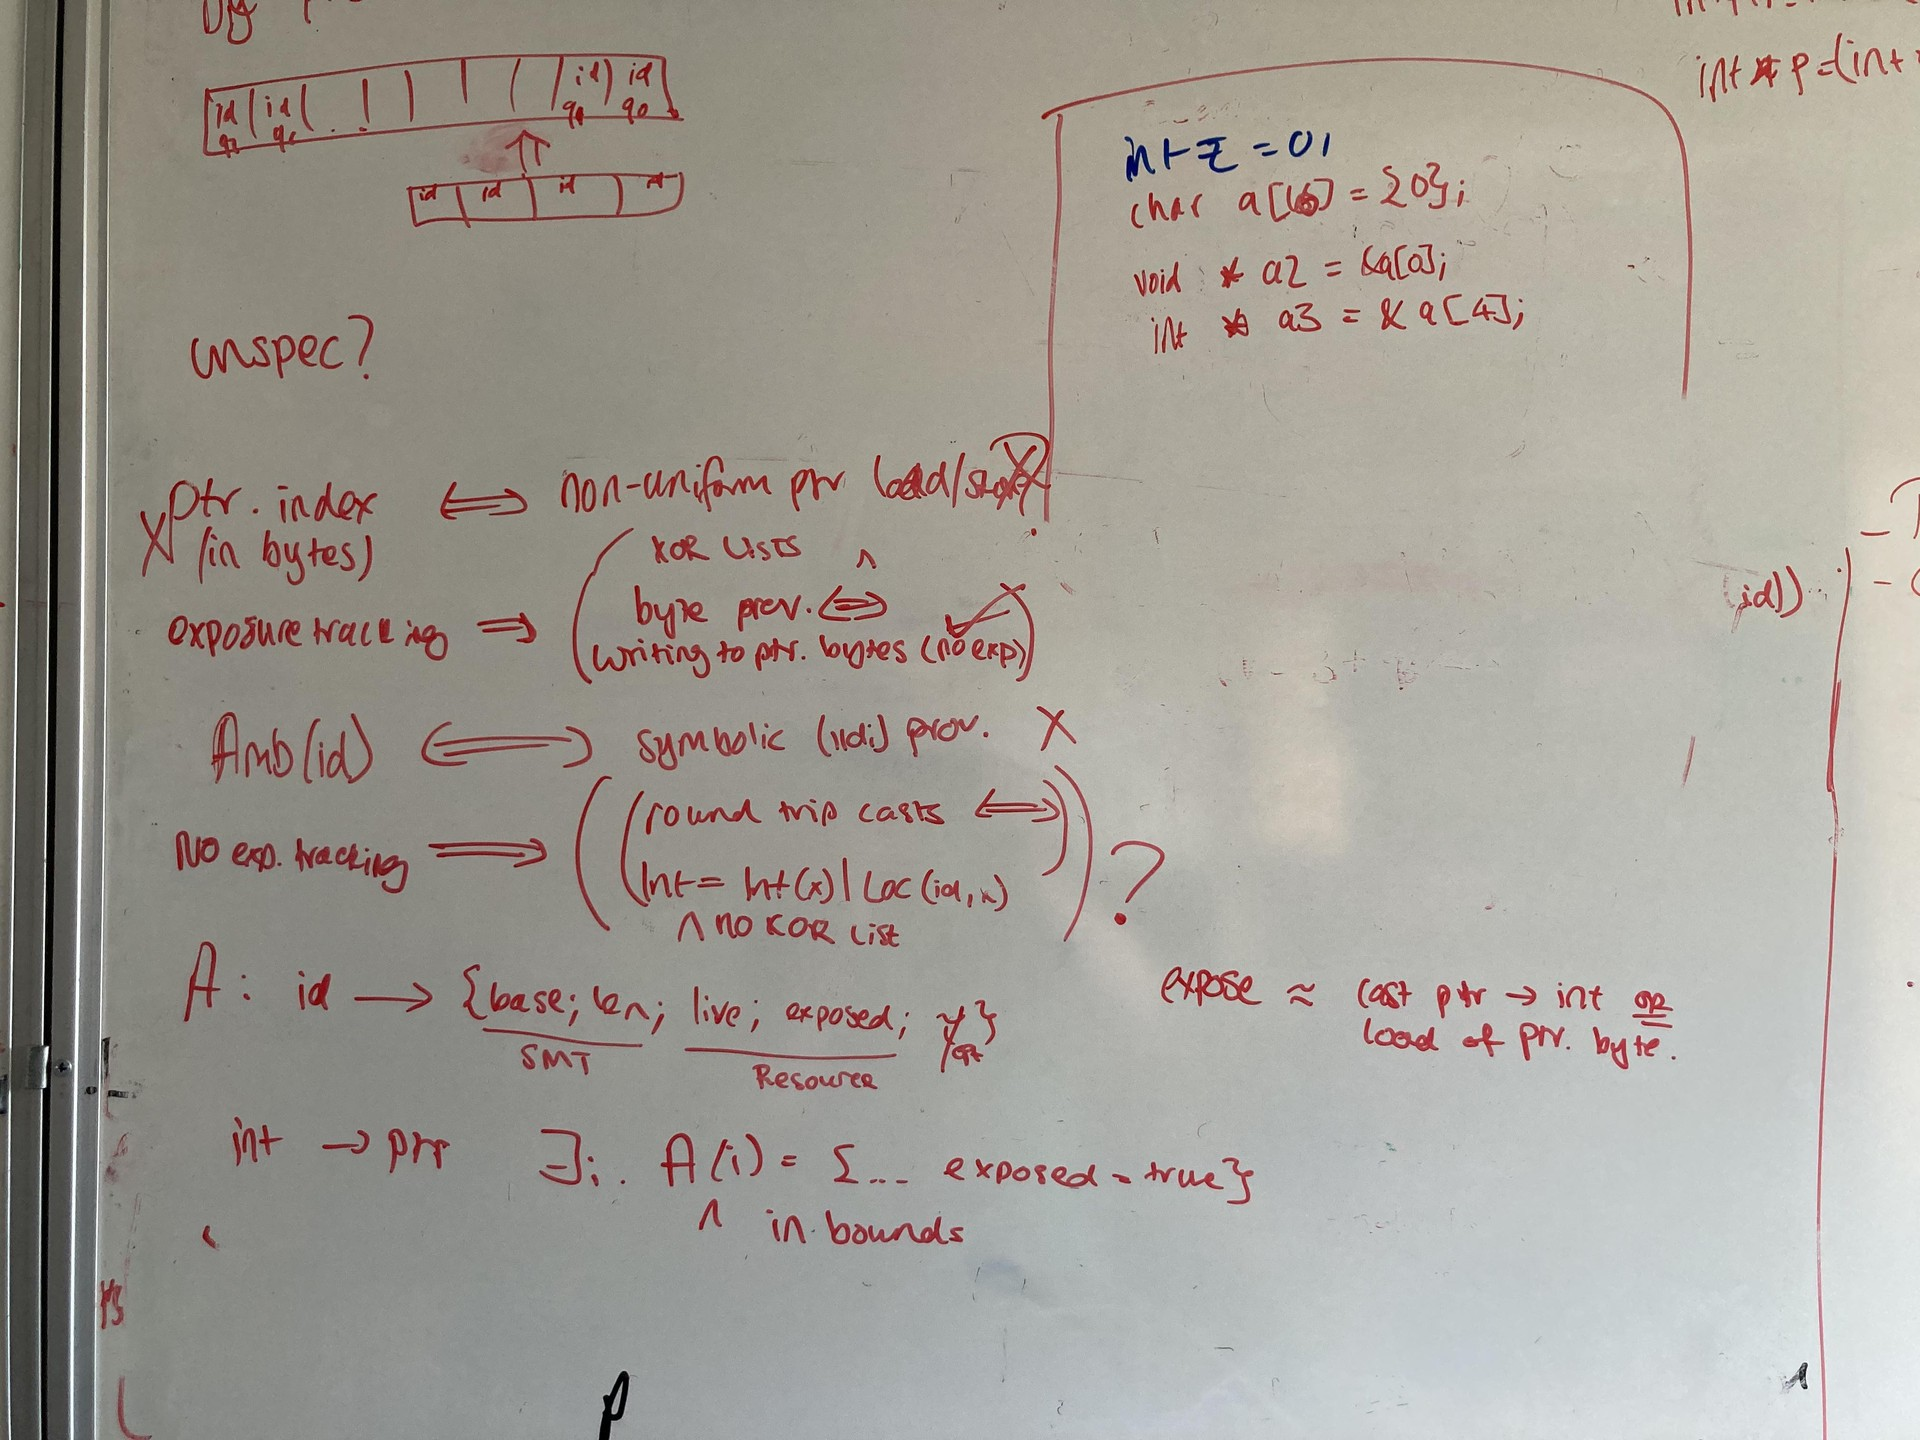
\includegraphics[width=\textwidth]{../misc/type-system-options.jpg}
\end{figure}


\section{Implementation}

Performance graph

\begin{figure}[h]
    \centering
    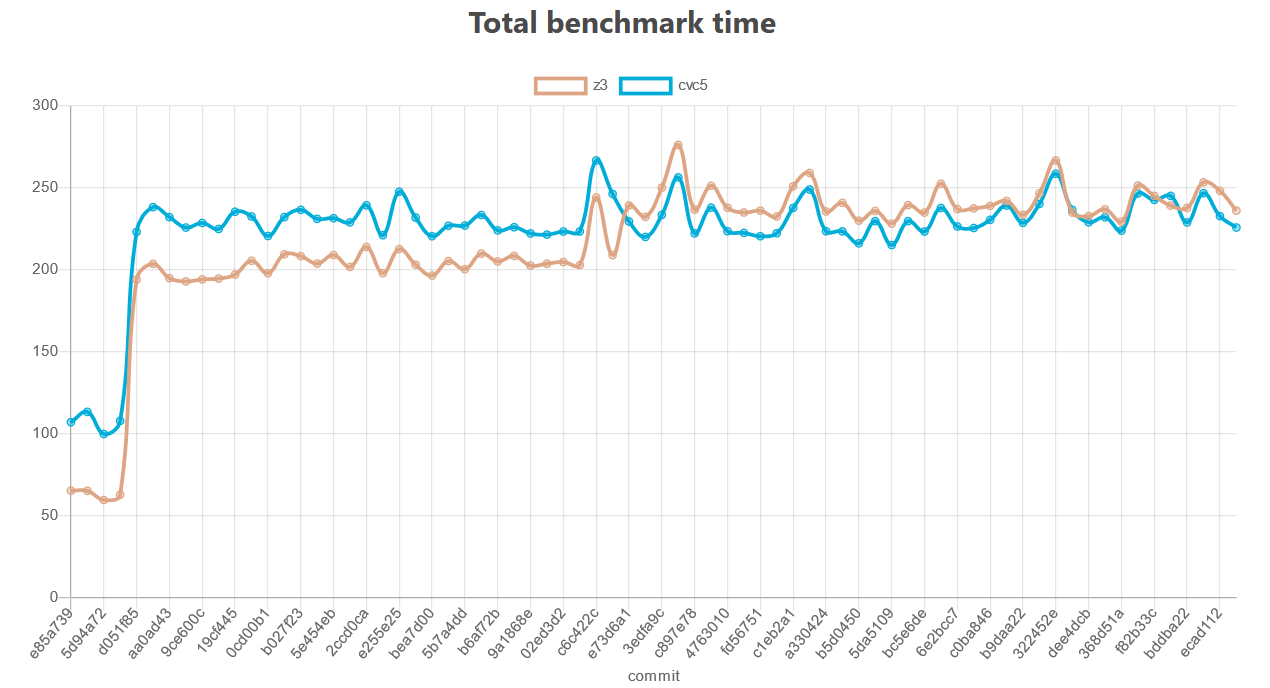
\includegraphics[width=\textwidth]{../misc/vip-performance-hit.png}
\end{figure}

\url{https://rems-project.githb.io/cerberus/dev/bench/}

\begin{comment}

\kl{Coq} is a very complex tool. Even its \kl{kernel}, which is only but a very small
fraction of it, is already quite complex: it relies on subtle implicit invariants, which
might not be properly maintained, especially when the code evolves.
In practice, around one critical bug is found every year.%
\sidenote{A \href{https://github.com/coq/coq/blob/master/dev/doc/critical-bugs}{compilation}
  of those is maintained by \kl{Coq}’s development team.}
Although it is in practice generally difficult to exploit these
and actually derive an inconsistency,
even less so inadvertently, simply relying on the \kl{De Bruijn criterion}%
\sidenote{Keeping a small, trusted kernel that is the only one responsible for the validity
of proofs.}
is not enough if one wants to trust \kl{Coq}.
Indeed, while \kl{CIC} is well-understood and has been widely studied,
this is much less true of the type theory actually implemented, \kl{PCUIC}.
Bugs therefore often creep in with the extra level of complexity coming with the implementation,
rather than being the consequence of a defect of pen-and-paper proofs.%
\sidenote{This is for instance the case of the completeness issue
  exposed in \cref{sec:bidir-pcuic-inductives}.}

These difficulties beg for a precise investigation of \kl{PCUIC}, from the heights of the
type system’s meta-theory, all the way down to the sophisticated details of the implementation.
Due to the complexity of the endeavour, it is not feasible on paper. Nor is it
desirable: if in the end we wish to implement a certified kernel, it is natural to do so
in a proof assistant, so that we can run that certified implementation.
The natural framework is thus the \kl{MetaCoq} project,
which aims at giving tools to reify and manipulate \kl{Coq} terms%
\sidenote{Or, maybe more accurately, \kl{Gallina}.}
inside \kl{Coq} itself. This gives the possibility to write down and certify
all kinds of procedures operating on these terms, the first to come to mind being of course
a type-checker. This way, we can have both the help and guarantees offered by
formal proofs inside a \kl{proof assistant}, and the possibility to execute
our implemented kernel.

There are two important caveats to this, though.
The first pertains to Gödel’s second incompleteness
theorem. Because of it, it is impossible to prove \kl{Coq}’s consistency
inside \kl{Coq} itself,
meaning that the meta-theoretical study can only be partial, since otherwise it would allow
a proof of consistency contradicting Gödel’s theorem. In
\kl{MetaCoq}, this blind spot manifests as an axiom assuming the
\kl{normalization} of \kl{PCUIC}, on which parts of the development relies.
The second caveat is that writing down a certified kernel is not enough.
Indeed, executing directly such a kernel in \kl{Coq}
would be much too slow to actually type-check any reasonably-sized term.
Rather, we must rely on extraction, a procedure which erases the
proof-related content of a certified program to only keep the algorithmically relevant one.
As this erasure itself is a complex transformation, \kl{MetaCoq} also incorporates a certified
erasure procedure.

In this part of the thesis,
I shall describe the portion of \kl{MetaCoq} which is relevant to it.
\Cref{chap:metacoq-general} gives a general overview of
the meta-theory of \kl{PCUIC}, with the main definitions, properties, and proof ideas.
My technical contributions to this part of the development is relatively minor,
mainly consisting of small patches. However, since I rely on that formalization
in my main contributions, it seems fitting to go over it.

\Cref{chap:kernel-correctness} concentrates on the formalization of bidirectional typing, as
presented in \arefpart{bidir}, and on the proof of correctness and completeness of
the kernel implementation based on it. This is my main technical
contributions to the \kl{MetaCoq} project.

Although I will not describe it here, there is more to \kl{MetaCoq}. The two main components
I will omit are Template \kl{Coq}, and the certified extraction procedure.
The first faithfully represents the actual abstract
syntax tree of \kl{Gallina} and a typing predicate for it,
gives a translation to the syntax used in the main theoretical development of \kl{PCUIC},%
\sidenote{Described in \cref{fig:metacoq-ast}.}
and shows that both notions of typing are equivalent.
It also provides facilities for quoting and unquoting of terms from
\kl{Coq} to \kl{MetaCoq}’s AST and back, in order to provide the possibility to write operation
on \kl{Coq} terms directly in \kl{MetaCoq} – including, of course, the certified kernel of
\cref{chap:kernel-correctness}.
The second component aims at certifyng the extraction procedure,
relating the semantics of the original and extracted programs.
The goal is to be able to extract the certified type-checker itself to an efficient one –
execution in \kl{Coq} is too inefficient if we wish to type-check realistic examples –,
but also more generally to improve \kl{Coq}’s current extraction.

Throughout the part, source files of the \kl{MetaCoq} project
and specific definitions or theorems are referenced respectively as follows:
\pcuicfile{Typing}, and \pcuicline{Typing}{typing}{188}. They link directly to the source
code of the project on \kl{GitHub} – on a branch dedicated to this thesis.

\end{comment}

%TC:ignore
% \pagelayout{fullwidth}
% \includegraphics{./figures/test.pdf}
% \pagelayout{margin}

\chapter{Formalized Meta-Theory of \kl(tit){PCUIC}}
\label{chap:metacoq-general}

\margintoc

Before we can attempt to build a certified kernel, we need a thorough meta-theoretical study
of the type system. This is necessary in order to show that the invariants used by the kernel – typically, well-formation of the objects it manipulates – 
are preserved during the type-checking algorithm.
The use of these invariants goes beyond correctness:
the cumulativity test used as a sub-routine by the \kl{kernel} needs to reduce terms, and,
since all functions in \kl{Coq} must be terminating,
this reduction is defined by well-founded induction on the \kl{normalization}
of well-typed terms.
Since evaluation is not normalizing on ill-typed terms, the mere \emph{definition} of the
cumulativity check relies on \kl{subject reduction} to be able to iterate reduction steps.

The properties under scrutiny in this chapter are not new,
and neither are the basic strategy of most proofs.
Indeed, the development roughly follows the architecture we already exposed in
\cref{sec:tech-properties}. The main difficulty is the scale: due to the
complexity of \kl{PCUIC}, even well-understood techniques are challenging to apply.
Moreover, subtleties that do not appear in a simpler setting become apparent –
typically pertaining to universe levels or general inductive types –,
demanding original ideas. Thus, rather than getting lost in
the gory details of the formalization which are best understood by looking at it
– and maybe replaying it –, we try and focus on describing these interesting subtleties.

In more details, we start with the main definitions : the syntax, cumulativity and typing
judgments (\cref{sec:meta-defs}). We follow with the basic
stability properties (\cref{sec:meta-stabilities}):
renaming, substitution, environment extension, etc.
Next comes the first important proof, that of confluence, and its multiple consequences
(\cref{sec:meta-confluence}). This leads to the properties pertaining to typing, culminating
with subject reduction (\cref{sec:meta-typing-prop}).
Finally, we discuss the place of normalization (\cref{sec:meta-normalization}).

\section{Setting up the Definitions: Terms, Cumulativity and Types}[Setting up the Definitions]
\label{sec:meta-defs}

\subsection{Terms}

First thing first: the syntax of terms, defined in \pcuicfile{Ast} and reproduced in \cref{fig:metacoq-ast}.

\begin{figure*}
  \coqfile{./code/PCUICAst.v}
  \caption{The Abstract Syntax Tree of terms in \kl{MetaCoq} (\pcuicline{Ast}{term}{194})}
  \label{fig:metacoq-ast}
\end{figure*}

It of course contains  the term formers introduced in \cref{chap:tech-intro}:
\coqe{tRel} for variables, \coqe{tAbs} for abstractions,
\coqe{tApp} for application, and \coqe{tProd} for dependent function types.
The syntax uses De Bruijn indices for binders – the integer argument of the \coqe{tRel}
term former –, but names are still recorded, mainly for printing purposes, directly in the
binders – the \coqe{aname} argument of \coqe{tProp} and \coqe{tAbs}.
There are also local definitions, in the form of the \coqe{tLetIn} constructor,
binding the term \coqe{b} of type \coqe{B} in \coqe{t}.

The \coqe{tSort} constructor is for sorts – what we have called universes earlier.
Its \coqe{Universe.t} argument represents its \kl{universe level}, which can be either $\Prop$
or an algebraic expression based on universe variables, in order to handle \kl{typical ambiguity}.

Next come \coqe{tVar} and \coqe{tEvar}, which
correspond respectively to named variables and existential variables.
These are ill-typed in the current notion of typing,
and thus ignored in most of the development. Still, they are kept to be as
faithful as possible to the representation of the \kl{Coq} kernel.
Indeed, the inductive \coqe{term} corresponds directly to the
\mintinline{OCaml}{constr} datatype used there.%
\sidenote{The only differences are that the latter uses
an n-ary application rather than a binary one, and casts that inform the \kl{kernel} as to
which cumulativity algorithm to use, but which is left out since we implement only one such
algorithm.}

Follow the three term formers \coqe{tConst}, \coqe{tInd} and
\coqe{tConstruct} all referring to previous definitions, stored in a \kl{global environment}.
The first corresponds to constants, that either have a body – definitions –
or do not – axioms. The next two are respectively for
inductive types and inductive constructors. Co-inductive and record types and
constructors are also represented by these term formers, the information contained in the
\coqe{inductive} argument is used to separate between them.
All of these can be \kl{universe polymorphic}, in which case they must be instantiated
with a list of universes – their \coqe{Instance.t} argument.

The two subsequent \coqe{tCase} and \coqe{tProj} are destructors for (co-)inductive types. The
latter is a \kl{projection}, used to destruct \kl{record types}. The former represents the
pattern-matching construction. Its main components are the \kl{predicate} \coqe{p}, the
\kl{scrutinee} \coqe{c} and the \kl{branches} \coqe{brs}. While it will appear more clearly
when giving the typing rule, let us note already that \coqe{p} and \coqe{brs} both contain not
only the body of the \kl{predicate}/\kl{scrutinee}, but also the context extension over which
they live, roughly corresponding to the variable bounds in the \kl{recursors} of \cref{sec:tech-cic}.
Thus, they represent a form of binding in the “primitive” way of a context extension, rather
than using Π-types or λ-abstraction. This is the new case representation alluded to
at the end of \cref{sec:bidir-pcuic-inductives}.

Finally, the two very similar \coqe{tFix} and \coqe{tCoFix} are for (co-)fixed-points. 
These can be mutual: the \coqe{mfix} argument is a list of definitions,
that can refer to each other.

\subsection{Cumulativity}

The next important definition is that of \kl{cumulativity}, given in \pcuicfile{CumulativitySpec}.%
\sidenote{The “Spec” part comes from the fact that this is the \emph{specification} of cumulativity,
by contrast to the algorithmic version encountered later on.}
It is stated in the \kl[declarative conversion]{declarative} \kl(conv){untyped} fashion,
akin to how we defined \kl{declarative conversion} in
\cref{fig:cic-uconv-beta,fig:cic-uconv-equiv,fig:cic-uconv-cong}.
This time, however, it is done relatively to
both a \kl{global environment} \coqe{Σ} and a context \coqe{Γ},
as these contain definitions that \kl{cumulativity} can unfold.

\kl{Cumulativity} is defined mutually with \kl{conversion}, because for instance when two Π-types
are compared for \kl{cumulativity}, their codomains are recursively compared for \kl{cumulativity},
but their domains are compared for \kl{conversion} instead.%
\sidenote{As explained in \cref{sec:tech-pcuic},
this is a consequence of the models justifying cumulativity.}
Since the two relations are extremely similar, they are actually fused in a single
inductive relation, \coqe{Σ ;;; Γ ⊢ t ≤s[pb] u}.
\AP This relation is indexed by a \intro{conversion problem} \coqe{pb : conv_pb}, which can take
the two values \coqe{Conv} and \coqe{Cumul}, so that \kl{cumulativity}
is actually \coqe{≤s[Cumul]} – and \kl{conversion} is
\coqe{≤s[Conv]}. This has the advantage that a lot of definitions and proofs
can be factored using \coqe{conv_pb}.
Moreover, using a simple boolean allows for case reasoning
when needed, which would be more complex if the index was \eg a relation.%
\sidenote{This used to be the case prior to the uniform introduction of \coqe{conv_pb}: the
relation was the one to be used at leaves to compare universes, which differed between 
\kl{conversion} and \kl{cumulativity}.}

\begin{figure}[h]
  \ContinuedFloat*
  \coqfile[firstline=3,lastline=12]{./code/PCUICCumulativitySpec.v}
  \caption{Pre-order rules (\pcuicline{CumulativitySpec}{cumulSpec0}{29})}
  \label{fig:meta-cumul-struct}
\end{figure}

\AP The first set of rules are the pre-order rules of \cref{fig:meta-cumul-struct}:
transitivity, symmetry and reflexivity. Note that symmetry restricts the \kl{conversion problem},
since only \kl{conversion} should be symmetric. Using this rule twice shows that 
\kl{conversion} is included inside \kl{cumulativity}.
Another important thing to note is that transitivity is somewhat restricted:
the middle term is required to be \intro{well-scoped},%
\sidenote{Expressed by the \pcuicline[Syntax]{OnFreeVars}{is\_open\_term}{253} predicate.}
\ie all its variables refer correctly
to either a binder or to the context \coqe{Γ}.
This is key when proving the equivalence between this notion of \kl{cumulativity} and the
algorithmic version that appears later on. Indeed, this equivalence relies on \kl{confluence},
which is only true on \kl{well-scoped} terms in \kl{PCUIC}. Thus, we need to know that
\kl(conv){declarative} \kl{cumulativity} only ever goes through \kl{well-scoped} terms,
which is exactly what this condition enforces.

\begin{figure}[ht]
  \ContinuedFloat
  \coqfile[firstline=44,lastline=48]{./code/PCUICCumulativitySpec.v}
  \caption{Example of congruence rule (\pcuicline{CumulativitySpec}{cumulSpec0}{29})}
  \label{fig:meta-cumul-cong}
\end{figure}

\begin{figure}[h]
  \ContinuedFloat
  \coqfile[firstline=15,lastline=29]{./code/PCUICCumulativitySpec.v}
  \caption{Cumulativity rules (\pcuicline{CumulativitySpec}{cumulSpec0}{29})}
  \label{fig:meta-cumul-cumul}
\end{figure}

Next come the rules of congruence. There are actually two kinds of them. The first are the
“standard” ones, similar to those of \cref{fig:cic-uconv-cong}. An example
is given in \cref{fig:meta-cumul-cong}.
More interesting are the rules of
\cref{fig:meta-cumul-cumul}, which implement “real” cumulativity. Rule \coqe{cumul_Sort} directly
implements subtyping between universes, while rules \coqe{cumul_Ind} and \coqe{cumul_Construct}
implement cumulativity of inductive types \sidecite{Timany2017}. The latter two apply respectively
to \emph{fully applied} inductive types and inductive constructors, that can be considered equal
if their arguments are one-to-one convertible, and their universe levels are correctly related.
This means that \eg the \coqe{nil} constructor of polymorphic lists \emph{always} satisfies that
\coqe{nil@{u} A} is convertible to \coqe{nil@{u'} A}, irrespective of the universe levels \coqe{u}
and \coqe{u'}.

\begin{figure*}
  \ContinuedFloat
  \coqfile[firstline=87,lastline=96]{./code/PCUICCumulativitySpec.v}
  \caption{Computation rules for destructors (\pcuicline{CumulativitySpec}{cumulSpec0}{29})}
  \label{fig:meta-cumul-dest}
\end{figure*}

Last are the rules for computation.
The three rules of \cref{fig:meta-cumul-dest} are for destructors, \ie applied functions,
pattern-matching on a constructor, and projections. The β rule for functions directly uses
substitution: \coqe|b{0 := a}| denotes the substitution of \coqe{a} for the variable of De Bruijn
index \coqe{0} in \coqe{b}. Similarly, the
\coqe{iota_red} function computes the substitution of the branch \coqe{br} by the arguments
of the constructor \coqe{args}.
Finally, the rule for projections simply selects the right field of the record.

\begin{figure*}
  \ContinuedFloat
  \coqfile[firstline=99,lastline=106]{./code/PCUICCumulativitySpec.v}
  \caption{Computation rules for definitions (\pcuicline{CumulativitySpec}{cumulSpec0}{29})}
  \label{fig:meta-cumul-defs}
\end{figure*}

The next three rules deal with definitions (\cref{fig:meta-cumul-defs}).
Rule \coqe{cumul_zeta} directly reduces a
let-binder into a substitution, while definitions are unfolded using \coqe{cumul_rel} and \coqe{cumul_delta},
respectively those of the local context or the \kl{global environment}. In the latter
case, the definition must be instantiated with a universe instance,%
\sidenote{A list of universe levels, corresponding to its polymorphic universe variables.}
which is denoted \coqe{@[u]}.

\begin{figure}[h]
  \ContinuedFloat
  \coqfile[firstline=108,lastline=119]{./code/PCUICCumulativitySpec.v}
  \caption{Computation rules for fixed-points (\pcuicline{CumulativitySpec}{cumulSpec0}{29})}
  \label{fig:meta-cumul-fix}
\end{figure}

The last rules (\cref{fig:meta-cumul-fix}) pertain to the reduction of (co-)fixed-points.
In all cases, they are unfolded in a guarded fashion, in order to avoid a non-terminating behaviour.
On fixed-points, this guard is that they have to be applied to a constructor,
and dually co-fixed-points are unfolded when
they are forced, either by a pattern-matching or a projection. In both cases, this ensures that
the unfolded (co-)fixed-point can reduce further, either by consuming the constructor of
its recursive argument, or by producing a constructor to be consumed by the destructor
that forced the unfolding.

\FloatBarrier
\subsection{Typing}

With the \kl{cumulativity} relation defined, we can turn to typing, defined in \pcuicfile{Typing}.
Similarly to \kl{cumulativity}, \pcuicline{Typing}{typing}{188}
is an inductively defined relation \coqe{Σ ;;; Γ |- t : T},
relative to a global environment \coqe{Σ} and a local context \coqe{Γ}.
The rules correspond roughly to ones we already went over in \cref{chap:tech-intro}.

\begin{figure}
  \ContinuedFloat*
  \coqfile[firstline=2,lastline=22]{./code/PCUICTyping.v}
  \caption{Functional fragment (\pcuicline{Typing}{typing}{188})}
  \label{fig:meta-typing-ccw}
\end{figure}

The first set of typing rules, given in \cref{fig:meta-typing-ccw},
pertain to the purely functional fragment. There are not many differences
there with respect to \cref{fig:ccw-typing}. Rule \coqe{type_Rel} looks up for the type of a
variable in the context, and ensures that said context is well-formed:
the \pcuicline{Typing}{wf\_local}{284} predicate corresponds to $\vdash \Gamma$,
but here as everything else it is relative to a global environment.
Rule \coqe{type_Sort} uses the \coqe{super} function to compute
the successor of an algebraic universe, and similarly Rule \coqe{type_Prod} uses
\coqe{sort_of product} to compute the universe level of a Π-type.%
\sidenote{This not only includes computing the maximum of two algebraic universes expressions,
but also handling the \kl{impredicativity} of the sort $\Prop$.}
Context extension with an assumption, \ie a variable without a body,
is written \coqe{Γ ,, vass na A}, and used as expected in Rules \coqe{type_Prod}
and \coqe{type_Lambda}. Finally, \coqe{type_App} is for application. It contains an
assumption that the product is well-formed, which is not strictly speaking needed once we
prove \kl{validity}, but is useful in some cases to provide a needed induction hypothesis.

\begin{figure}
  \ContinuedFloat
  \coqfile[firstline=23,lastline=27]{./code/PCUICTyping.v}
  \caption{Local definitions (\pcuicline{Typing}{typing}{188})}
  \label{fig:meta-typing-letin}
\end{figure}

The rule for local definitions, given in \cref{fig:meta-typing-letin}, is similar to the one
for λ-abstractions, with the only difference that the body too is typed, and that the context
is extended with a definition, \ie a variable with a body, which is written \coqe{Γ,, vdef na b B}.

\begin{figure*}
  \ContinuedFloat
  \coqfile[firstline=28,lastline=42]{./code/PCUICTyping.v}
  \caption{Globally defined terms (\pcuicline{Typing}{typing}{188})}
  \label{fig:meta-typing-genv}
\end{figure*}

Next (\cref{fig:meta-typing-genv}) are the three rules performing look-ups in
the \kl{global environment}, respectively constants – \coqe{type_Const} –, inductive types –
\coqe{type_Ind} – and inductive constructors – \coqe{type_Construct}. In all cases the
term should be declared in the \kl{global environment}, the context well-formed
– since these are leaves of a term –,
and the universe instance given should respect the constraints coming from the
entry in the \kl{environment} – this is the \coqe{consistent\_instance\_ext} predicate.

\begin{figure*}
  \ContinuedFloat
  \coqfile[firstline=43,lastline=58]{./code/PCUICTyping.v}
  \caption{(Co-)inductive destructors (\pcuicline{Typing}{typing}{188})}
  \label{fig:meta-typing-idest}
\end{figure*}

The rules of \cref{fig:meta-typing-idest} are the ones for the destructors of (co-)inductive
types. Rule \coqe{type_Case} is somewhat similar to \ruleref{rule:bool-ind}. First,
the \kl{scrutinee} should be of an inductive type, declared in the global environment.
Next, the \kl{predicate} and \kl{branches} should all be well-typed
in the appropriate context – obtained by combining the information stored in
\coqe{p} or \coqe{brs}, with that retrieved from the entry in the environment corresponding to
the \kl{scrutinee}'s type.
Finally, \pcuicline{Typing}{case\_side\_conditions}{159} handles universe instances, checks
that the elimination is allowed%
\sidenote{This is where \kl{PCUIC} enforces computational irrelevance of proofs,
by imposing the so-called
“singleton elimination” criterion, which ensures that only inductive
types of a certain specific shape – sub-singletons – can be matched on to build proof relevant
content, so that that content cannot actually depend on the value of a proof.}…
The second rule, \coqe{type_Proj}, is somewhat similar, albeit a bit simpler: the \kl{scrutinee}
should still be some applied co-inductive/record type, and the type is constructed by
substitution from the projection information.

\begin{figure}
  \ContinuedFloat
  \coqfile[firstline=59,lastline=76]{./code/PCUICTyping.v}
  \caption{(Co-)fixed-points (\pcuicline{Typing}{typing}{188})}
  \label{fig:meta-typing-fix}
\end{figure}

The last typing rules for terms are those for (co-)fixed-points,
given in \cref{fig:meta-typing-fix}. They are almost identical,
the main part amounts to checking that the types and bodies of all
the mutual definitions are well-typed.
The \pcuicline{Typing}{wf\_fixpoint}{118} and \pcuicline{Typing}{wf\_cofixpoint}{145}
predicates both check that the definitions are on
the same block of mutually-defined (co-)inductive types, and that these are of the right kind –
inductive for \coqe{tFix} and co-inductive for \coqe{tCoFix}.
Finally, the \coqe{fix_guard} and \coqe{cofix_guard} predicates correspond to the guard condition,
ensuring that the definitions do not endanger \kl{normalization}. We come back to those in
\cref{sec:meta-normalization}.

\begin{figure}
  \ContinuedFloat
  \coqfile[firstline=77,lastline=81]{./code/PCUICTyping.v}
  \caption{Cumulativity (\pcuicline{Typing}{typing}{188})}
  \label{fig:meta-typing-cumul}
\end{figure}

The final rule (\cref{fig:meta-typing-cumul}) is that which uses \kl{cumulativity} as just defined
to change the type of the term, \eg the equivalent of \ruleref{rule:cic-cum}.

From the definition of \pcuicline{Typing}{typing}{188}, two more pervasively used definitions
follow. We have already encountered \pcuicline{PCUICTyping}{wf\_local}{284},
asserting that a local context is well-formed.
Its sibling predicate \pcuicline{PCUICTyping}{wf}{439}%
\sidenote{Often replaced by \pcuicline{PCUICTyping}{wf\_ext}{444},
an extension that in addition takes into account the universes of the current definition.}
asserts that the \kl{global environment} is well-formed. It ensures not only that all definitions
are properly typed, but also of the validity of various information
related to inductive types – in particular the positivity criterion which ensures that inductive
definitions are well-founded –, and universe polymorphism.

\section[Stabilities]{The Easy Properties: Stabilities}
\label{sec:meta-stabilities}

With the main definitions set up, we can turn to the properties that we collectively called
stabilities in \cref{sec:tech-properties}. These assert that \kl{cumulativity} and typing
as just defined are stable by various ubiquitous operations: extension of the local context%
\sidenote{\pcuicfile[Conversion]{WeakeningConv} and \pcuicfile[Typing]{WeakeningTyp}.}
and global environment,%
\sidenote{\pcuicfile[Conversion]{WeakeningEnvConv} and \pcuicfile[Typing]{WeakeningEnvTyp}.}
and substitution, not only for terms,%
\sidenote{\pcuicfile[Conversion]{InstConv} and \pcuicfile{Substitution}}
but also for universe variables.%
\sidenote{\pcuicfile[Conversion]{UnivSubstitutionConv} and \pcuicfile[Typing]{UnivSubstitutionTyp}}

\AP One last property falling in the section of low-hanging fruits as well
is the fact that well-typed terms are \kl{well-scoped}.%
\sidenote{\pcuicfile{ClosedTyp}.}
%, that is that if \coqe{Σ ;;; Γ |- t : T}
%then all free variables of \coqe{t} appear in \coqe{Γ}.
This \kl{well-scoping} conditions appears
in the transitivity rule for \kl{cumulativity}
(\cref{fig:meta-cumul-struct}) and is a hypothesis for many lemmas.

All of these are proven by induction on the typing derivation.
While the proof by themselves are not very surprising, the formalization of the definitions
deserves a few comments.

The first point to note is that while the weakening and substitution operations are defined
directly by induction on the syntax of terms, the proofs are not done directly
on those definitions. Rather, \kl{MetaCoq} uses notions of renaming and instantiation inspired
by the σ-calculus \sidecite{Abadi1991,Schaefer2015}, as functions from natural numbers
to natural numbers for renamings, and to terms for instantiations.
\kl{Weakening} and \kl{substitution} then correspond respectively to a specific form of
renaming and of instantiation, and the stability for the former those follows from
more general versions for the latter.
For instance, \kl{weakening} is but a consequence of general stability by
(unconditional) renaming, as presented in \cref{prop:stab-renaming}.
This approach makes it easier to handle the complex binding structures
present in the syntax of \kl{PCUIC}, which require parallel substitution or
lifting by a whole context at once,
operations that are easier to handle in the general framework of the σ-calculus.

More interestingly and novel, the same approach is taken also for \kl{well-scoping}:
\kl{MetaCoq} generalizes that predicate into a way of lifting
any boolean function on natural numbers – seen as a property of variables – to a boolean function
on terms.\sidenote{This is \pcuicline[Syntax]{OnFreeVars}{on\_free\_vars}{71}.}
This makes it easy to relate the σ-calculus
to \kl{well-scoping} assumptions, \eg to show that if two substitutions \coqe{σ} and \coqe{σ'}
agree on the free variables of a term \coqe{t}, then the application of \coqe{σ} and \coqe{σ'}
to \coqe{t} are equal.

\begin{figure}[h]
  \coqfile{./code/PCUICSubstitution.v}
  \caption{Well-formed substitution (\pcuicline{Substitution}{subslet}{44})}
  \label{fig:meta-subslet}
\end{figure}

A last point of interest is the definition of a well-formed substitution, a predicate called
\pcuicline{Substitution}{subslet}{44}.
Indeed, the usual typing judgment for substitutions
is of the form $\Delta \vdash \sigma \ty \Gamma$, meaning that
$\sigma$ maps each assumption $(x : A) \in \Gamma$ to a term $t$ such that
$\Delta \vdash t \ty \multisubs{T}{\sigma}$. But in our setting we must account for variables
that can be \emph{defined} in $\Delta$. This leads to the definition of a well-formed substitution as in \cref{fig:meta-subslet}.
A similar definition, called \pcuicline[Syntax]{InstDef}{well\_subst}{65}, is also available for
instantiations.

\section[Confluence]{Things Get Serious: Confluence}
\label{sec:meta-confluence}

\begin{figure*}[ht]
  \coqfile{./code/PCUICReduction.v}
  \caption{\kl{One-step reduction} and \kl{reduction}}
  \label{fig:meta-red}
\end{figure*}


As in \cref{sec:tech-properties}, the next step is to define \kl{reduction} and
establish its properties.
An excerpt of the definitions is given in \cref{fig:meta-red}:
\kl{reduction} is \pcuicline{Reduction}{red}{303},
defined as as the reflexive, transitive closure
of \kl{one-step reduction} \pcuicline{Reduction}{red1}{18}.
The former is written \coqe{Σ ;;; Γ |- t ~>* u}, and the latter
\coqe{Σ ;;; Γ |- t ~> u}.

\subsection{Parallel reduction}
\label{sec:metacoq-parred}

\AP The proof of \kl{confluence} follows the standard Tait-Martin-Löf approach as exposed by
\sidetextcite{Takahashi1995}. It relies on a notion of \intro{parallel reduction}
$\mathord{\intro*\parred}$, which can reduce multiple redexes present in a term $t$ in parallel.
As an example, the rules for application are given in \cref{fig:parred-app}.
\begin{marginfigure}
  \begin{mathpar}
  \inferrule
    {t \parred t' \\ u \parred u'}
    {t\ u \parred t'\ u'} \and
  \inferrule
    {t \parred t' \\ u \parred u'}
    {(\l x : A.\ t)\ u \parred \subs{t'}{x}{u'}}
  \end{mathpar}
  \caption{Parallel reduction for application}
  \label{fig:parred-app}
\end{marginfigure}
The generic congruence
rule allows reduction to happen in parallel in both the function and argument. Moreover,
if the function is an abstraction, a β step can also be fired simultaneously 
with those. Note that this does \emph{not} allow reducing further redexes
that would be produced by the substitution. For instance, we do not have
\[(\l f : \Nat \to \Nat . f\ 0)\ (\l x : \Nat. x) \parred 0\]
because the redex $(\l x : \Nat. x)\ 0$ only appears after a first step of substitution.

\kl{Parallel reduction} has two interesting properties. First, it
is related to \kl[reduction]{standard reduction}.

\begin{lemma}[Parallel reduction and reduction]
  \label{lem:parred-red}
  We have $\ored \subset \mathord{\parred} \subset \mathord{\fred}$.

  This implies that if \kl{parallel reduction} is \kl{confluent}, then so is \kl{reduction}.
\end{lemma}

\AP But the interesting characteristic of \kl{parallel reduction}, which \kl{reduction}
does not satisfy, is the
\intro{diamond property}, a strong version of local confluence,%
\sidenote{
  Which says that if $t \ored t_1$ and $t \ored t_2$ then there exists $t'$ such that $t_1 \red t'$
  and $t_2 \red t'$.}
which contrarily to it implies \kl{confluence} even in the absence of \kl{normalization}.
Thanks to \cref{lem:parred-red} above, in order to establish \kl{confluence} of 
\kl{reduction}, it suffices to show this \kl{diamond property}.

The proof idea goes as follows. First, show that \kl{parallel reduction} is substitutive, in
the following sense.
\begin{lemma}[Parallel reduction is substitutive]
  If $t \parred t'$ and $u \parred u'$ then
  $\subs{t}{x}{u} \parred \subs{t'}{x}{u'}$.
\end{lemma}
\AP This allows to define a \intro{best parallel reduct} $\intro*\bestredop$,
which reduces \emph{all} possible redexes in parallel,%
\sidenote{ For instance $\bestred{(\l x : A.\ t)\ u}$ is $\subs{\bestred{t}}{x}{\bestred{u}}$.
}
and to show that it is really a best reduct.
\begin{lemma}[Triangle property]
  Given a term $t$, if $t \parred t'$ then $t' \parred \bestred{t}$.
\end{lemma}

\begin{marginfigure}
  \centering 
  \begin{tikzcd}
      t \arrow[triple,dr] \arrow[triple,d] & \\
      t' \arrow[triple,r] & \bestred{t}
  \end{tikzcd}

  \begin{tikzcd}
    & t \arrow[triple,dl] \arrow[triple,dr] & \\
    t_1 \arrow[triple, dr] && t_2 \arrow[triple,dl] \\
    & \bestred{t} &
  \end{tikzcd}
  \caption{The triangle and diamond properties, as diagrams}
\end{marginfigure}

This is enough to get the diamond property, because any two parallel reducts of a term $t$
both reduce to $\bestred{t}$ \emph{in one step}. This basically amounts to firing in both reducts
all the redexes that could have been triggered but have not been.

\begin{minipage}{\textwidth}
\begin{lemma}[Diamond property]
  Given a term $t$ and $t_1$, $t_2$ such that $t \parred t_1$ and $t \parred t_2$, there exists
  $t'$ such that $t_1 \parred t'$ and $t_2 \parred t'$.
\end{lemma}
\end{minipage}

From this, it follows by a bit of diagram chasing that \kl{parallel reduction} is confluent,
and thus that \kl{reduction} is.

\begin{minipage}{\textwidth}
\begin{theorem}[\kl{Confluence} of \kl{reduction}]
  \kl{Reduction} is \kl{confluent}, that is if $t \red t_1$ and $t \red t_2$ then there exists
  $t'$ such that $t_1 \red t'$ and $t_2 \red t'$.
\end{theorem}
\end{minipage}

Note that it can directly be shown without resorting to \kl{parallel reduction} that \kl{reduction}
is \emph{locally} confluent. However, in the absence of \kl{normalization}
to apply Newman’s lemma, this
is not enough to ensure \kl{confluence}. But, while we can hope that \kl{normalization} holds for
well-typed term, it is clearly false on untyped terms. Yet, it is crucial to get confluence on
those, as otherwise we would not be able to establish \kl{injectivity of type constructors} and thus
\kl{subject reduction} with our untyped notion of \kl{cumulativity}.
Thus, this detour through \kl{parallel reduction} is really unavoidable.

\subsection{Formalizing Takahashi’s proof}

The previous section sets down a quite precise plan, that we can almost directly follow in \kl{MetaCoq}. There is one important subtlety though: because of local definitions, \kl{reduction}
depends on contexts, so these must be taken into account in \kl{parallel reduction}. But
bodies of definitions should also be reduced by \kl{parallel reduction},
and so the actual relation is between pairs of a context and a term,
something like $\Gamma, t \parred \Gamma', t'$.

Apart from this difficulty%
\sidenote{And the technicality of defining $\bestredop$ in a terminating fashion, 
which is done using the \kl{Equations} plugin \cite{Sozeau2019a}.}%
\margincite{Sozeau2019a}
the plan can be followed quite closely.
\kl{Parallel reduction} is defined as \pcuicline{ParallelReduction}{pred1}{241} in
\pcuicfile{ParallelReduction}. Then the diamond property is proven in \pcuicfile{ParallelReductionConfluence} – $\bestredop$ is \pcuicline{ParallelReductionConfluence}{rho}{697},
and the diamond property itself is \pcuicline{ParallelReductionConfluence}{pred1\_diamond}{4421}.
Finally, \pcuicfile{Confluence} goes back from this to properties of \kl{reduction}, concluding
with its \kl{confluence} (\pcuicline{Confluence}{red\_confluence}{3959}).

\section[The Road to Subject Reduction]{Reaping the Fruits: the Road to Subject Reduction}
\label{sec:meta-typing-prop}

With \kl{confluence} proven, it is time to reap the fruits. First,
\kl(conv){declarative} \kl{cumulativity},
as used to define typing, can be related to \kl(conv){algorithmic} \kl{cumulativity}. This entails
many useful consequences, including \kl{injectivity of type constructors}.
A series of important properties then follow, culminating with \kl{subject reduction}.

\subsection{Algorithmic cumulativity}

The first use of confluence is to relate \kl(conv){declarative} \kl{cumulativity}
as used to define typing to \kl(conv){algorithmic} \kl{cumulativity} –
\pcuicline{Cumulativity}{cumulAlgo}{31} –
defined as reduction to terms related by the \kl{α-pre-order} $\alphleq$.%
\sidenote{The generalization of \kl{α-equality} to handle \kl{cumulativity}.}
But in the setting of \kl{PCUIC} this relation, called \pcuicline{Equality}{leq\_term}{382} in
the formalization, is far from being trivial to define!
It needs to handle algebraic universe levels, but also polymorphic inductive types. Moreover,
it is parameterized over the relation used to compare universes, so that it can also be used
to express “pure” \kl{α-equality}%
\sidenote{Meaning that the terms can differ only on binder names, but that their universe
must be syntactically the same rather than related using the constraints present in the
environment.}
when instantiated with equality rather than universe comparison.

To show that \kl{algorithmic conversion} is equivalent to \kl{declarative conversion},
\kl{confluence} is the major ingredient, but it is not enough. Instead, we also need to show
that \kl{reduction} interacts well with this \kl{α-pre-order}.

\begin{lemma}[The \kl{α-pre-order} is a simulation
    (\pcuicline{Confluence}{red1\_eq\_term\_upto\_univ\_l}{838})]
  \begin{marginfigure}
    \centering
    \begin{tikzcd}
        t \arrow[d, "1" very near end] \arrow[r, phantom, "\alphleq" description] &
        t' \arrow[d, dashed, "1" very near end] \\
        u \arrow[r,phantom,"\alphleq" description] & u'
    \end{tikzcd}
    \caption{Simulation, as a diagram}
    \label{fig:alphleq-sim}
  \end{marginfigure}
  If $t \alphleq t'$ and $\Gamma \vdash t \ored u$ then there exists some $u'$ such that
  $\Gamma \vdash t' \ored u'$ and $u \alphleq u'$.
\end{lemma}

While the proof
is still relatively straightforward since $t$ and $t'$ have the same structure, it becomes
much more challenging if we wish to integrate extensionality rules such as η-equality or 
strict propositions%
\sidenote{Two features present in \kl{Coq} but not yet in \kl{MetaCoq}, exactly due to this
kind of difficulties.}
into $\alphleq$.

Combining this simulation property with \kl{confluence},
transitivity of \kl(conv){algorithmic} \kl{cumulativity} follows,
and finally its equivalence with \kl(conv){declarative} \kl{cumulativity}.

\begin{theorem}[Equivalence of the presentations of \kl{cumulativity}]
  \kl(conv){Algorithmic} and \kl(conv){declarative} \kl{cumulativity} are equivalent.
\end{theorem}

This equivalence is the main theorem of \pcuicfile{Conversion} – 
one direction is \pcuicline{Conversion}{cumulSpec\_cumulAlgo}{3680},
and the other is \pcuicline{Conversion}{cumulAlgo\_cumulSpec}{190}.
That central file also proves multiple variants of
\kl{injectivity of type constructors}.
For instance, \kl{injectivity of function types} is \pcuicline{Conversion}{ws\_cumul\_pb\_Prod\_Prod\_inv}{718},
and the stronger form used in \kl(bidir){completeness} of bidirectional typing
(\cref{lem:conv-red-tycons}) is \pcuicline{Conversion}{ws\_cumul\_pb\_Prod\_r\_inv}{686}.

\subsection{Reaping the fruits}

With injectivity settled, we can get to the main properties of typing.
The easiest is \pcuicline{Validity}{validity}{453},
asserting that if $\Gamma \vdash t \ty T$ then $T$ is a well-formed type in $\Gamma$.
The second is that typing is insensible to names (\pcuicline{Alpha}{typing\_alpha}{1009}):
if two terms differ only in variable names and one is typable, then so is the other.
And, finally, comes \pcuicline{SR}{subject\_reduction}{3072}.

While the main proofs of these theorems are far from simple,%
\sidenote{That for \kl{subject reduction} needs more than 1500 lines for the main induction!}
an important part of the proof effort is actually required ahead of them
in \pcuicfile{Inductives} and \pcuicfile{InductiveInversion},
in order to show that the various contexts, substitutions, applications, etc.
that appear in conversion and typing for inductive types behave as expected.

Regarding \kl{subject reduction}, a caveat applies. Because the “positive”
presentation of co-fixed-points does not preserve types, as explained in
\cref{sec:pcuic-records}, only the “negative” presentation based on projections is allowed.
In practice, this means
that the typing rule \pcuicline{Typing}{type\_case}{241} of \cref{fig:meta-typing-idest}
forbids the \kl{scrutinee} from being of a co-inductive type.%
\sidenote{This is part of the \pcuicline{Typing}{case\_side\_conditions}{159}.}
Hence, while \kl{reduction} and \kl{conversion} take this presentation into account,%
\sidenote{See the \pcuicline{CumulativitySpec}{cumul\_cofix\_case}{158}
constructor in \cref{fig:meta-cumul-fix}.}
thus showing at least that it is confluent, it can never appear in a well-typed term.

An alternative solution, which would allow an easier transition away from today’s positive
co-inductive types, is to see co-inductive scrutinees as effectful terms
and restricts predicates allowed
for dependent elimination to be linear, following \sidetextcite[0em]{Pedrot2017}.
This approach is not formalized in \kl{MetaCoq} – yet –, but the project
provides a natural setting to explore this kind of questions in all their gritty details
before working towards an actual implementation in \kl{Coq}.

\section[Normalization]{Gödel’s Thorn in the Side: Normalization}
\label{sec:meta-normalization}

One last important property remains: \kl{normalization}. In \kl{PCUIC}, the key constraint to
ensure it is the \kl{guard condition}, to which (co-)fixed-points are subject in order to
ensure that they are well-founded – see \cref{sec:pcuic-ind}.
However, due to Gödel’s second incompleteness theorem, if \kl{PCUIC} is \kl(log){consistent}
then it cannot prove its own \kl(log){consistency}.
But if \kl{normalization} were provable, then so would be \kl(log){consistency}.
There is therefore no hope to give a guard condition and prove that it entails \kl{normalization}.

\subsection{An abstract guard condition}

\begin{figure}[h]
  \coqfile{./code/PCUICGuard.v}
  \caption{The \pcuicline{Typing}{guard}{54} axiom}
  \label{fig:meta-guard}
\end{figure}

Instead, \kl{MetaCoq} takes a different approach. The existence of a \kl{guard condition} is
\emph{assumed} in an abstract, axiomatic fashion – see \cref{fig:meta-guard} –
and used in typing – see \cref{fig:meta-typing-fix}.
Similarly, \pcuicfile{GuardCondition} assumes properties of this axiomatic guard: it
should be stable by universe and term substitution, extension of the \kl{global environment},
cumulativity of the local context insensible to names, and, most importantly, stable by
reduction.

These abstract properties are enough to handle the whole development outlined above. In other
words, given any notion of \kl{guard condition} that satisfies the criteria of
\pcuicfile{GuardCondition}, typing satisfies \kl{injectivity of type constructors},
\kl{validity}, \kl{subject reduction}… Thus, our abstract approach provides a precise
characterization of the properties the \kl{guard condition} needs to satisfy in order
for typing to be well-behaved.

In particular, since the trivial guard condition
that is always true fulfils the requirements, none of the aforementioned
properties rely on \kl{normalization} – or \kl(log){consistency} of the theory.
Thus, \kl{PCUIC} is a \kl[safety]{safe} programming language, \emph{unconditionally}.

\subsection{The normalization axiom}

\begin{figure}[h]
  \coqfile{./code/PCUICSN.v}
  \caption{The \pcuicline{SN}{normalization}{36} axiom}
  \label{fig:meta-sn}
\end{figure}

But of course we need more. In particular, if we wish to define a convertibility check
inside \kl{Coq}, which only allows to define terminating functions,
we must know that reduction is terminating. Once again, we axiomatize the necessary
axiom of (strong) \kl{normalization}, as given in \cref{fig:meta-sn}.
Note that this axiom takes exactly the form we gave to \kl{normalization}
in \cref{prop:normalization}, as the accessibility of any well-typed term for
co-reduction. This is done under the assumption that the global context is well-formed,
otherwise it could contain \eg non-positive inductive types which
could be used to define non-terminating terms.

Using this axiom, it is possible to prove \kl(log){consistency} of \kl{PCUIC}, as shown in
\safefile{Consistency}. The rough idea of the proof is that given for \cref{prop:log-cons},
\ie to deduce \kl(log){consistency} from \kl{canonicity}.
However, instead of proving \kl{progress} directly we rely on a proven-complete function 
computing \kl(red){weak-head} normal forms implemented as part of the type-checker.%
\sidenote{Which can be seen as a constructive witness of \kl{canonicity}!}
Assuming an inhabitant \coqe{t} of $\P b : \Prop.\ b$%
\sidenote{Corresponding to the \kl{MetaCoq} term
\coqe{tProd b (tSort Prop_univ) (tRel 0)}.}
in any axiom-free global environment \coqe{Σ}, the proof extends
\coqe{Σ} with the empty inductive type $\Empty$, use \coqe{t} to construct a
\kl(red){weak-head} normal inhabitant of that type, and from this finally derive a contradiction.
\chapter{Building a Certified Kernel}
\label{chap:kernel-correctness}

\margintoc

With the meta-theory set down, we can turn to building a kernel – and proving that it is
correct. The first step (\cref{sec:kernel-bidir})
is to move from the declarative specification of
\cref{chap:metacoq-general} to a bidirectional presentation,
closer to the kernel we wish to implement.
Once this specification is set down, we can get to the kernel itself.
\cref{sec:kernel-subroutines} goes over the implementation of the \kl{global environment} and the
\kl{cumulativity} check, and \cref{sec:kernel-typing} describes the type-checker.
Finally, \cref{sec:kernel-beyond-typing} describes two extra functions belonging to the safe
\kl{kernel}: re-typing, and checking of \kl{global environment}.

I personally contributed the formalizations of \cref{sec:kernel-bidir},
the \kl(bidir){completeness} part of \cref{sec:kernel-typing} –
by modifying the pre-existing proven-\kl(bidir){sound} type-checker –,
and heavily modified re-typing – part of \cref{sec:kernel-beyond-typing}.

\section{Formalized Bidirectional Typing}
  [Bidirectional Typing, Formalized]
\label{sec:kernel-bidir}

We already saw the main theoretical ideas around our approach to bidirectional typing in
\arefpart{bidir}, so let us get to their implementation in the formalization.

\subsection{Definitions}

Before we can get to the definition of typing, we must go through the small
\pcuicfile[Bidirectional][BD]{EnvironmentTyping}, which is dedicated to refining a few
definitions on contexts in the bidirectional setting. First,
in the case of a definition \coqe{Γ,, vdef na b T},
\coqe{wf_local} enforces that \coqe{T} is a well-formed type, and that
\coqe{b} has type \coqe{T}. In the bidirectional setting we want to use constrained inference
$\pity{\uni}$ for the first, and checking for the second, but the generic definition
on which \coqe{wf_local} is built%
\sidenote{Called \coqe{All_local_env}.}
only allows for a single parameter – instantiated with \coqe{typing} in the case
of \coqe{wf_local}.
Similarly, we need a definition expressing that a context $\Delta$ is well-formed
\emph{over another context $\Gamma$}, but which does not enforce $\Gamma$ to be well-formed
\textit{a priori} – \eg something more precise than simply $\vdash \Gamma , \Delta$. This
allows to stay faithful to McBride’s discipline%
\sidenote{Taken from \textcite{McBride2018}, see its exposition in \cref{sec:bidir-mcbride}.}%
\margincite{McBride2018}
when typing context extensions,
by only demanding that the extension is well-formed, but not the initial segment.%
\sidenote{Which is an input, and thus should not be re-checked.}

The bidirectional typing judgment is defined in
\pcuicfile[Bidirectional][BD]{Typing}, as a set mutual defined inductive predicates:
one for inference, one for checking, and one for each constrained inference, \eg respectively
sorts, Π-types and inductive types. The definition of the predicates themselves
is very close to that of \cref{fig:ccw-bidir-infer,fig:bidir-ccw-other} for the
functional fragment, the main innovation being that constrained inference – 
written \coqe{Σ ;;; Γ |- t |>Π (na,A,B)} for Π-types –
takes the variable name, domain and codomain of the inductive type as three separate arguments,
which our pen-and-paper notation did not make explicit.
The predicates defined in \pcuicfile[Bidirectional][BD]{EnvironmentTyping} are used in the
definition of inference for the \coqe{tCase} node, where we want to ensure that the
context extensions used to type the \kl{predicate} and \kl{branches} are well-formed.

Regarding the notions of computation, the definitions of \kl{constrained inference} use
\kl{full reduction} rather than \kl{weak-head reduction}, mainly because MetaCoq currently
lacks a treatment of the latter adequate for our needs.%
\sidenote{In particular, a standardization theorem is missing,
which would be needed to show the analogue
of \cref{lem:conv-red-tycons} for weak-head reduction.}
As for \kl{cumulativity}, the \kl(conv){algorithmic} variant is used in the \kl{checking} rule,
but this is relatively irrelevant,
since the equivalence between both presentations of \kl{cumulativity}
appears much earlier in the development than bidirectional typing.

Maybe more interesting from the formalization point of view is how we obtain a usable
induction principle. This is a common issue in \kl{MetaCoq}: while
\kl{Coq} is able to detect that our inductive definitions are well-founded,
the default generation is often unable to derive a sensible induction principle,
and neither are the \coqe{Scheme} specialized commands. This is due to their nested
character, \ie the presence of lists and records containing recursive instances
of the inductive types as arguments to the type constructors.
The bidirectional typing predicate is the paroxysmal example of this, as it
reaches the limit of expressiveness offered by
\kl{Coq}’s inductive types: it is not only nested, but also mutual.
We thus have to prove our desired induction principle by
hand. To do so, we introduce a notion of “generic” typing object
\pcuicline[Bidirectional][BD]{Typing}{typing\_sum}{256},
together with a notion of size for such a typing object,
and finally show the induction principle
\pcuicline[Bidirectional][BD]{Typing}{bidir\_ind\_env}{312}
by well-founded induction on that size.

This induction principle is not as strong as we might expect, as it does not provide the extra induction hypothesis on inputs that would go with McBride's discipline.
Ideally, we could use this discipline
in order to thread the well-formation invariants, giving stronger induction
hypotheses. I did not try to take this path and prove such a strong induction principle,
as it did not seem so easy: it would effectively correspond to an inline proof
of \kl{validity}.
Instead, the discipline is reflected in the choice of the predicates proven by induction.
For instance, in the case of soundness, the mutually proven predicate for inference
is \coqe{wf_local Σ Γ -> Σ ;;; Γ |- t : T}, and more generally
assumptions are added as pre-condition for all inputs.
Still, I conjecture that such a strong induction principle should be provable, if the need
would arise, and might be nice in order to factor proofs, by showing once and for all that
the rules follow the discipline correctly.

\subsection{Equivalence with undirected typing}

\kl(bidir){Soundness}%
\sidenote{Bidirectional typing implies undirected typing, akin to \cref{thm:corr-ccomega}.}
is shown in \pcuicfile[Bidirectional][BD]{ToPCUIC}.
The main proof is by induction on the derivation,
its key point being to show that well-formation invariants are preserved, and in particular
that all contexts that are constructed are valid.

There is one particular difficulty linked to the \coqe{tCase} constructor, and the question
of its representation evoked at the very end of \cref{sec:bidir-pcuic-inductives}.
More precisely, the issue is related to the fact that case nodes store the universe
instance and parameters of the inductive type being matched upon, in order to be able to
construct the context in which the \kl{predicate} and \kl{branches} are typed.
In undirected typing, the hypothesis on the \kl{scrutinee} is that it should be of some type
\coqline|mkApps (tInd ci.(ci_ind) p.(puinst)) (p.(pparams) ++ indices)|
where \coqe{ci.(ci_ind)}, \coqe{p.(puinst)} and \coqe{p.(pparams)}
are respectively the inductive type being matched upon, its universe instance, and its
parameters – all stored in the case node –, and \coqe{indices}
are free. From the point of view of bidirectional typing, this rule is invalid:%
\sidenote{It is not mode-correct \cite{Dunfield2021}.}%
\margincite{Dunfield2021}
because \coqe{indices} is free, this cannot be turned into a checking premise, but it also
cannot be directly turned into inference, or even constrained inference, because it is
not free enough due to the presence of \coqe{p.(pparams)} and \coqe{p.(puinst)}.
The solution is still to turn it into an inference premise
\coqe/Σ ;;; Γ |- c |>{ci} (u,args)/, and to compare the inferred universe instance \coqe{u}
and parameters – the first part of the list \coqe{args} – to those stored in the node, \eg
\coqe{p.(puinst)} and \coqe{p.(pparams)}. But it requires some work to
show that this relation between the two lists of parameters is enough to use the second part
of \coqe{args}, the inferred indices, in place of \coqe{indices} above.

In the opposite direction, \kl(bidir){completeness}%
\sidenote{Undirected typing implies bidirectional typing, akin to \cref{thm:compl-ccomega}.}
is also proven by induction, once we have used
the injectivity properties of \pcuicfile{Conversion} to show that
inference of a type related by \kl{cumulativity} to a sort, Π- or inductive type implies
constrained inference of the corresponding kind.
In order to simplify proofs in the case of projections,
\kl(bidir){soundness} is used in conjunction
with \kl{validity}, but this could probably be avoided, making the two proofs independent.

\subsection{Properties of bidirectional typing}

As we did in \cref{thm:unique-inf}, we show that two inferred types have a common reduct in
\pcuicfile[Bidirectional][BD]{Unique}. While the proof requires some playing with
well-scoping predicates,%
\sidenote{
  To relate the reduction used to defined \kl{constrained inference} and the one on which most lemmas
  around confluence are stated, which is defined directly on well-scoped terms.}
it is conceptually \emph{much} simpler than the direct proof of \pcuicfile{Principality},
which shows the existence of \kl{principal types} without going through bidirectional typing.
Indeed, due to the difficulty of the proof,
for quite some time only a weaker version was proven.
This version that if $T$ and $T'$ are both types
for the same term $t$ then there exists a third $T''$ which
is both a type for $t$ and smaller than 
$T$ and $T'$ for cumulativity.

Finally, \pcuicfile[Bidirectional][BD]{Strengthening} shows strengthening.
Its first important property is that if $\Gamma \vdash t \ity T$ then
$T$ can only use variables appearing in either $t$ or in the types of $\Gamma$
(\pcuicline[Bidirectional][BD]{Strengthening}{infering\_on\_free\_vars}{487}),
which is \emph{not} true in general in undirected typing.%
\sidenote{Consider for instance $n : \Nat \vdash 0 : (\l x : \Nat.\ \Nat)\ n$: $n$ appears in the
type, but neither in the body of the term nor any types in the context.}
It then goes on with the proof that bidirectional typing is stable under any renaming, while
\pcuicfile{RenameTyp} only shows stability of undirected typing under unconditional renaming.
Finally, we get to the proof of \pcuicline[Bidirectional][BD]{Strengthening}{strengthening}{989}
\textit{per se}, once we have shown that strengthening is indeed a well-formed renaming.

\section{Before Typing: Environment Querying and Cumulativity Checking}[Before Typing]
\label{sec:kernel-subroutines}

Before we can get to typing, we need to have a look at its two main sub-routines:
querying the \kl{global environment}, and \kl{cumulativity} check.

\subsection{Abstract environment}

The type and \kl{cumulativity} checking algorithms both need to query the \kl{global environment},
for two main purposes: retrieving information about previous definitions
of constants and inductive types, and checking that (in)equalities between
universe expression hold.

While this might seem anecdotal,
a surprisingly important amount of time is spent in the actual checker
on the second problem, which requires a form of shortest-path algorithm
on a graph obtained from the universe constraints, in order
to detect the presence of negative cycles.
These correspond to violations of the universe stratification.
\kl{MetaCoq} implements such an algorithm, with a proof that it is correct – \ie sound and complete –, meaning that
the algorithm answers “yes” exactly when there is a mapping from universe levels to integers satisfying
all constraints declared in the environment.
More details on this can be found in \sidetextcite[][Section 3.3]{Sozeau2020}.

Sadly, said algorithm is too naive to be actually run on reasonable examples: it is currently the main
performance bottleneck of the extracted type-checker. Similarly, the representation of the
\kl{global environment} as a list of definitions is too naive to allow for efficient lookups –
\kl{Coq} uses hash maps instead.
While we hope to replace that naive implementation with a more efficient but still certified one,
for the moment it is convenient to be able to plug an uncertified but efficient implementation
into the extracted type-checker. To do so, we rely on abstract interfaces for the
\kl{global environment}, containing all the possible queries we need to perform,
presented in \safefile{WfEnv}. The naive implementation is shown to be a valid implementation of
that interface in \safefile{WfEnvImpl}.

\subsection{Cumulativity checking}

The most important sub-routine of the type-checker is the test of \kl{cumulativity} between two terms.
The naive way to perform this, since we assume \kl{normalization}, would be to brutally normalize terms,
and compare normal forms up to \coqe{leq_term}.%
\sidenote{The extension of \kl{α-equality} to handle \kl{cumulativity}.}
But this strategy does not scale as soon as definitions are present, because it
eagerly unfolds all of these, resulting in a very inefficient test.
\kl{MetaCoq} implements a more practical strategy, which coarsely does the following:
\begin{enumerate}
  \item reduce both terms being compared to \kl(red){weak-head} normal form
    \emph{without unfolding any definition};
  \item if the two heads match, recursively compare sub-terms;
  \item if the two heads do not match, or if the recursive sub-term comparison failed, check if
    an unfolding is possible which would unblock one of the terms, and if yes, unfold it and
    go back to the first step.
\end{enumerate}
This means that the \kl{cumulativity} test must itself resort to a \kl{weak-head reduction}
function.

The difficulty with those functions is that they do not operate by a simple structural induction on
terms. Rather, they are defined using a complex abstract machine, operating on terms decomposed into
a sub-term and a stack. The termination of that abstract machine is shown using a
dependent lexicographic pre-order, which handles both the well-founded reduction order given by
\kl{normalization}, a structural order on sub-terms and stacks corresponding to a given term, and
the different phases of the algorithm.
A detailed description of this algorithm and its formalization%
\sidenote{In files \safefile{SafeReduce} for the implementation of \kl{weak-head reduction}, and
\safefile{SafeConversion} for the cumulativity checker.} is given by Théo Winterhalter,
who implemented it,%
\sidenote{It was only proven sound at the time. Jakob Botch Nielsen
wrote most of the completeness proof.
}
in his PhD thesis \sidecite[][Chapters 21-24]{Winterhalter2020}.

An interesting point that the test of \kl{cumulativity} and that of typing have in
common, is the way they handle their propositional content. First, because
we want to avoid issues linked with proof-irrelevance,
in most of the formalization definitions are in \coqe{Type},
including the reduction, conversion and typing relation.
But in the verified \kl{kernel} we want to enforce the
separation between propositional and relevant content. Thus, we use explicit squashing —
written $\| T \|$ – to cast a type into a proposition.%
\sidenote{Technically,
  $\| T \|$ is defined as a record of type $\Prop$ with a single field of type $T$.}
The main elimination of propositional content into the relevant world we rely on that
of accessibility, so that we can define \kl{reduction} and \kl{cumulativity} by well-founded induction. As customary in dependently typed code, we also use elimination of falsity in
inaccessible branches.

Second, we write code using the \kl{Equations} plugin, which lets us write the
relevant part of the definition in direct style, but to leave proofs to be filled-in using the
proof-mode. The definitions are given in monadic style, relying on what looks like the error monad:%
\sidenote{Given a type of errors $E$, the functor associated with that monad is $T \mapsto T + E$,
its unit is the left injection, and its bind $x >>= f$ either propagates $x$ if it is an error, or applies $f$ otherwise.}
the \kl{cumulativity}- and type-checker return a valid output, or an error message. However, since
we wish the functions to be correct by constructions, they must also return a proof, either a
witness for the positive answer, or a proof of impossibility in the negative case.
This means that the bind of the monad must actually perform a proof when re-raising the error,
in order to propagate the impossibility witness.%
\sidenote{For instance, if we are typing some \coqe{tProd na A B} and the call to typing for \coqe{A} 
fails, we must transform a proof that \coqe{A}
cannot be well-typed into a proof that \coqe{tProd na A B}
as a whole cannot either.}
At function definition, this is hidden by notations, so it feels like we are actually using a
monad, but under the hood proof obligations are generated each time we use a bind.

\section{Sound and Complete Inference}
\label{sec:kernel-typing}

Given the work already done in \cref{sec:kernel-bidir}, the definition of a
type checking algorithm \safefile{TypeChecker}
itself is rather straightforward: it follows closely
the structure laid out by the mutually defined bidirectional judgments, and
poses no termination issue as \kl{cumulativity} does, since it
operates by induction on the structure of the term.
Actually, rather than a type-checker, the main function we define is
\safeline{SafeChecker}{infer}{1323}, which performs type inference,%
\sidenote{
  Which is decidable thanks to our \kl{Church-style} syntax.}
from which we can easily define type-checking.

In more details, the function takes as inputs:
\begin{enumerate}
  \item an abstract environment implementation;
  \item a \kl{global environment} implemented using that implementation;
  \item a context, and a squashed proof that it is well-formed;
  \item a term
\end{enumerate}
and it returns either a type and a (squashed) proof that the term infers that type, or
an error and a proof that the term cannot infer any type, using the inductive type presented in
\cref{fig:meta-error-mon}.
\begin{figure}
  \coqfile[firstline=1,lastline=4]{./code/PCUICSafeTyping.v}
  \caption{The “error monad” used for \safeline{SafeChecker}{infer}{1323}’s return type}
  \label{fig:meta-error-mon}
\end{figure}
Thus, the function is sound and complete by construction.
In fact, we cannot separate
the definition from the soundness proof, since the conversion checker
expects a well-typed term as input in order to be terminating when it is called.

\begin{figure*}
  \coqfile[firstline=6]{./code/PCUICSafeTyping.v}
  \caption{Definition of \safeline{SafeChecker}{infer}{1323} (excerpt)}
  \label{fig:meta-infer}
\end{figure*}

\cref{fig:meta-infer} gives – an excerpt of – the algorithm.
%
For a variable \coqe{tRel n}, it checks that the variable is bound in
\coqe{Γ}, returns its type when it is, and fails otherwise.
%
In the case of a sort \coqe{tSort u}, it checks that the universe is well-formed in the current
environment, and returns a sort at the next level when it is.
%
In that of a dependent function type \coqe{tProd na A B}, it computes the sort of
\coqe{A} and \coqe{B} – in the context extended by
\coqe{na:A} –  using the \coqe{infer_type} sub-routine,%
\sidenote{Defined beforehand in an “open recursion” flavour, \eg as a function taking \coqe{infer}
as argument.}
and builds from those the sort of the product using \coqe{sort_of_product}.
Functions are similar.
%
The cases of \coqe{tLetIn} and \coqe{tApp} clearly show the bidirectional
structure. For instance, in
\coqe{tApp t u}, one needs to infer the type \coqe{ty} of \coqe{t},
then reduce it to some \coqe{tProd na A B} using the
\coqe{reduce_to_prod} function, and finally check that \coqe{u} has
type \coqe{A}.
%
All underscores \coqe{_} in the terms denote proof obligations, that are filled later on
in tactic mode. Although they are hidden, the monadic notations \coqe{;;}
and \coqe{raise} also contain underscores for the propagation of completeness
information.%
\sidenote{For instance, \coqe{raise e} is syntactic sugar for \coqe{TypeError_comp e _}.}

Interestingly, the proofs of \kl(bidir){completeness} use uniqueness of inferred types a lot.
To see why, consider \eg the case of an application $t\ u$ where the recursive call succeeds on $t$
– say it infers a product type $\P x : A.\ B$ – but the one on $u$ fails – giving us a proof $p$
that $u \cty A$ is absurd. We want to raise an error, and thus need to prove
that $t\ u \ity T$ for any $T$ is absurd.
An inversion on that last hypothesis gives some $A'$ and $B'$ such that
$t \pity{\P} \P x : A'.\ B'$ and $u \cty A'$.
But this second property cannot be directly fed $p$, because the type against which $u$ checks is
different! We thus need to use the two inference judgments and uniqueness to conclude that in
fact $A \conv A'$, and thus that $u \cty A$,
which this time we can the use to derive a contradiction from $p$.

\section{Beyond Typing: Environment Checking and Re-Typing}
\label{sec:kernel-beyond-typing}

There are two more functions defined in \kl{MetaCoq} that are very close to the type-checker.

\subsection{Re-Typing}

The first, which is defined in \safefile{SafeRetyping}, aims at computing a type for a term
which is known to be well-typed. While this seems tautological, it is not: the aim is
to extract relevant content out of propositional one. This is useful in practice in \eg
the extraction procedure, which maintains the invariant that it operates on well-typed terms,
but at times needs to actually compute types to decide whether terms should be erased.

This is also different from standard inference,
because knowing \textit{a priori} that the term under consideration is well-typed allows to
skip a lot of checks. For instance, to re-type an application $t\ u$, it suffices to infer a
product type $\P x : A.\ B$ for $t$, and to return $\subs{B}{x}{u}$, since we know that $u$
has type $A$.

In order to be useful, this re-typing procedure needs to compute a \kl{principal type}, and
thus its definition was quite complex prior to the formalization of bidirectional typing,
effectively inlining a proof of uniqueness of types. Instead, bidirectional typing
simplifies greatly both the definition of re-typing and its proof of correctness, by
clarifying its specification:
instead of computing a principal type out of any type,
the function should compute an unsquashed inferred type out of a squashed one.

\subsection{Environment Checking}

The second thing we need to handle is the verification that a whole \kl{global environment}
is well-formed. While the main thing to check is that all definitions are well-typed,
there are quite a few more things to be done: checking universes constraints, that inductive
definitions are strictly positive, that the variance information used by universe polymorphism is
valid… All these are covered in \safefile{SafeChecker}.
%TC:endignore

\pagelayout{wide} % No margins
\addpart{Engineering}
\label{part:eng}
\pagelayout{margin} % Restore margins

So far I have discussed the formalisation of \kl{CN}, the formalistaion and
implementation of its memory model, \kl{CN-VIP}. In both those sections,
guiding design choices and implementation decisions at each stage was the need
to strike a balance of expressiveness, performance and ergonomics,
fundamentally motivated by designing a \emph{capable} verification tool. Not
only that, at several stages, the theory was able to inform or clarify
implementation related issues, such as the complexity of adding new features,
lifting existing restrictions, or substantially improving performance.

In this part, I will take a step back and focus more on what it takes to build
a \emph{usable} verification tool. Though not as theoretically intruiging or
elegant as some of the material in the previous chapter, this is where just as
much, if not more, of the difficulty lies in achieving \kl{CN}'s goal of being
maintainable by kernel programmers (\cref{sec:cn-goals}).

It start with the source repository for any mature C project, such ask
\kl{pKVM}. It intentionally lives in the Linux kernel, indeed in many respects
this is an advantage. It is an unignorable reminder that C in the real word
however does not come neatly packaged up into isolated files of ISO grammar
conforming translations units. Aside from the myriad extensions that it relies
on, as well as non-ISO conforming C features, the inclusion chain of one file a
few hundred lines long can stretch \emph{eleven} directories up and total
around 65,000 lines of C after preprocessing. Mature industrial projects like
GCC and Clang have spent years optimising their front-ends to deal with this
complexity at speed, which creates a large gap between it, and robust,
empirically validated, but ultimately academic tools such as \kl{Cerberus}.

Thankfully, there is an alternative to simply adding features to the
\kl{Cerberus} frontend until it can handle a substantial number of GCC and
Clang fragments. In our experience, the set of features used by a particular
directory of files, such as the \kl{pKVM} project are relatively small, and can
be manually extracted by copying files, commenting out unused features, and
flattening directory hierarchies. Whilst this is possible, it is tedious, slow,
error prone and extremely time consuming, taking days to perform by hand,
making it very difficult to update once code is updated. Doing so trades-off
implementation and intellectual effort for grunt work and drudgery, which is a
step in the right direction, albeit no more practicable.

Faced with this, and the awareness of tools such as clang-format, which can
format complex projects of C++ code, including macros, and other Clang based
tools for linting and refactoring, I developed a tool which could automate the
aforemention drudgery. Analagous to tree-shaking for JIT-compiled interpreted
languages, I call the method \intro{tree-carving}, which given a root file in a
repository, extracts out the files in the transitive dependency of that root,
and comments out anything not used.\sidenote{Such a strategy works for most
sensibly formatted code with each top-level declaration on its own line. For
code which does not fit this, input validation will reject the program rather
than produce erroneous output.} It comments out code to preserve line numbers,
and works with macros too. Since \kl{CN} specifications are comments too, and
could get lost inside other comments, I also wrote a comment simplifier to undo
such nested comments.

Even with reasonable input, the challenges continue. One of the early
challenges \kl{CN} faced was that of allocation for function arguments. Though
intuitively, a programmer might model allocations for parameters as being
created by the \emph{callee}, early versions of \kl{CN} relied on
\kl{Cerberus}' elaboration allocating storage for function arguments at the
\emph{caller}, per callsite. This significantly degraded the experience of
writing specifications and proofs because the programmer had to specify that
functions did not mutate arguments at the callsite. Kayvan Memarinan fixed this
by creating a parallel mode of elaboration to support the more intuitive model.

Influenced by \kl{Cerberus}'s decision to model C integers as unbounded with
constraints, \kl{CN} originally adopted a similar design, and used to verify
the \kl{pKVM}'s buddy allocator, as mentioned in \sidetextcite{pulte2023cn}.
However, this soon became cumbersome due to the use for frequent bit
manipualation idioms in \kl{pKVM}'s page table walker, because expressing these
idioms on integers then required the frequent use of lemmas to handle the
(undecidable) non-linear arithmetic. This prompted an overhaul of \kl{CN} to
work with bit vectors as its fundamental integer type.

My contributions to this thread began as I attempted to update the buddy
allocator to handle a very early version of \kl{VIP}, which coincided with the
move to bit-vectors, \emph{and} a change in the inference scheme. Alongside
this, this was my first serious use of \kl{CN} and separation logic, and I did
not have the benefit of the helpful \kl{CN tutorial} to serve as less steep
cliff to ascend. To top it all off, the underlying code of the buddy allocator
had been updated, unbeknownst to anyone at the time (we did not have
performance benchmarking) \kl{CN} became dramatically slower, and at the time
had no ability to track source location information across the majority of its
pipeline. Whilst the attempt seems foolish and doomed from the start, it
clarified a few things we needed to improve upon.
\begin{itemize}
    \item Source location information.
    \item Regression testing.
    \item Peformance benchmarking.
    \item Switchable major transitions.
    \item A tutorial and worked examples.
    \item Upating proofs one aspect at a time.
\end{itemize}

As result of this failed attempt, I came to appreciate all the above. I ended
up spending about one month plumbing through source location information
throughout the core datatype in \kl{CN}, as well as fixing the lexer and
parser to be more robust and have extensible error messages.

I also identified a particularly difficult challenge which any verification
tool based on an internal representation needs to deal with is relating errors
back to the source code user wrote. This is particularly evident with SMT
counter-examples which are not minimal, consistent, nor easy to translate back
to the source. Aside from this, even in the absence of \kl{VIP} related
performance issues, \kl{CN} is still about an order of magnitude slower than we
would like it to be, though the causes of this are not clear, the plan of being
able to rely on performant SMT solvers with decidable queries has not paid off
quite as well as we would have liked.

\chapter{Tree-carving: Taming C Respositories}\label{chap:tree-carver}

\margintoc{}

In this chapter, I will explain why we need a tree-carver for C repositories,
by referring to the mounting challenges we were facing scaling \kl{Cerberus} to
handle large repositories. After that, I will explain the features of C which
make this a particularly challenging endeavour, mostly centred on macros and
the C preprocessor. I will also explain why it is very desirable to \emph{not}
input preprocessed C code into verification tools such as \kl{CN} (constants,
and column information). Lastly, I will show how, extending prior work
significantly, I built a Clang-based tool which meets almost all the
requirements we sought, enough to not be the primary bottleneck to verifying
code in large projects anymore. Lastly, I will explain the limitations of the
current approach (struct fields, cross-translation-unit carving), and ways this
may be remedied in the future.

\section{Need for tree-carving}

I will use the \kl{pKVM} page-table code as the motivation for the chapter.
It lives in the folder arch/arm64/kvm/hyp/pgtable.c, and consists of some simple
functions like the one below, for converting a page-table entry to a physical
address.

% c-tree-carve -r kvm_pgtable_hyp_map arch/arm64/kvm/hyp/pgtable.c -n 0

\cfile[fontsize=\footnotesize,breaklines,lastline=7]{code/pgtable.c}

It also includes more complicated functions such the one below which uses function
pointers, arguments, and flags in a struct to effectively create a closure, with
which to call a parametric page-table walking function.

\cfile[fontsize=\footnotesize,breaklines,firstline=9]{code/pgtable.c}

This code is not suitable to be input to \kl{Cerberus} because of the fact
is uses features it does not support. However, these features are not at
all obvious from just looking at the code; one would expect the only features
used are macro constants, and regular C declarations for types and functions.

Let us start with \cinline{KVM_PTE_ADDR_MASK}. This is defined using another
macro, \cinline{GENMASK}.

\cfile[fontsize=\footnotesize,breaklines,lastline=2]{code/kvm_pte_addr_mask.c}

In turn, \cinline{GENMASK} is defined using two macros, in separate file. The
second of these, \cinline{__GENMASK} is the one which defines the constant in
the expected way as a bit-shifting expression. However, the first,
\cinline{GENMASK_INPUT_CHECK}, relies on two other macros
\cinline{BUILD_BUG_ON_ZERO} and \cinline{__isconstexpr} and a compiler
intrinsic, \cinline{__builtin_choose_expr}.

\cfile[fontsize=\footnotesize,breaklines,firstline=3,lastline=14]{code/kvm_pte_addr_mask.c}

The \cinline{__isconstexpr} macro is defined in yet another file. I do not
understand how this works, and in any case, \kl{Cerberus} rejects it.

\cfile[fontsize=\footnotesize,breaklines,firstline=16,lastline=23]{code/kvm_pte_addr_mask.c}

The GCC built-in \cinline{__builtin_choose_expr} happens to take to expressions
as its arguments, but in general this is not the case. For example,
\cinline[breaklines,breakafter=_]{__builtin_types_compatible_p} takes two \emph{types} as
its argument. Such built-ins require editing the parser and elaboration to
support, and cannot be abstracted easily.

Lastly, \cinline{BUILD_BUG_ON_ZERO} uses the expression to try to construct an
anonymous struct with a bit-field of that size, since 0-width bit-fields are
not allowed, this will trigger a build error. Bit-fields are not supported by
\kl{Cerberus} either.

\cfile[fontsize=\footnotesize,breaklines,firstline=25,lastline=26]{code/kvm_pte_addr_mask.c}

Whilst the use of robust compile-time checks is laudable, the features
involved, the trail of dependencies of macros across different files and the
lack of \kl{Cerberus} front-end support for them makes them a non-starter to
even ignore when verifying code with \kl{CN}.

Remember, this is all just for
\cinline{KVM_PTE_ADDR_MASK}. In this case, there is a simple workaround
(redefine the \cinline{GENMASK} macro to not do any compile time checks). In
general, it is not is not possible to tell if a particular part of the code is
ignorable, or used by the code one wishes to verify. This is particularly
inconvenient because it then becomes difficult to distinguish whether a
particular feature is unavoidable and worth implementing in \kl{Cerberus}, or
just an incidental block to parsing, but otherwise safely ignored.

In other words, \emph{if parsing fails on a file, we are forced to implement
the construct in the parser, regardless of whether or not is is used later,}
which is not an efficient use of engineering capacity. As seen above, Linux
headers and macros frequently contain such constructs, so the issue persists
even after preprocessing.

\section{Challenging preprocessor and C features}

One may think that preprocessing will sidestep this issue, because unused
macros (and accompanying unsupported features) will not be pasted into the
code.

Unfortunately, whilst this does avoid the myriad problems of doing dependency
analysis on macros, it comes with trade-offs. Take the \cinline{GENMASK} macro
above. If expanded fully into each use site, the code to verify would be
littered with unsupported features. The structure of the macros and its
dependency, (the fact that there is one part which is a compile-time check, and
another which computes the expression we care about) would be lost, making it
harder to spot what to redefine and where for the purposes of proof.

Preprocessing would also corrupt source location information for
columns.\sidenote{Line directives keep the line information accurate, and
comments can be preserved with the right options} Whilst this is already lost
by the \kl{Cerberus} front-end, it would make it irrecoverable if \kl{Cerberus}
were to upgrade its
lexer.\sidenote{\href{https://github.com/rems-project/cerberus/issues/393}{Cerberus\#393}}

Preprocessing will also flatten the directory structure on the original
repository, making it more difficult to relate any output back to the code it
came from. Initially, we assumed that this sort of dependency analysis would be
quite expensive, so the idea was that a user would run the carving once,
annotate the carved code, and then merge the changes back into the source
repository, for which point preserving file structure may be
helpful.\sidenote{The alternative would be to create patches based on the line
directives in the single preprocessed files.}

However, analysing a non-preprocessed file is also fraught with difficulty.
Unfortunately, macros are not simply `find-and-replace' abstractions, but can
support conditionals, defining, un-defining and re-defining, as well as be
constructed dynamically with token-pasting. Macros are not stored as part of
the abstract syntax tree and so whether or not it was possible to recover
dependency information from them was an open question.

Aside from the preprocessor, C features such as forward declarations, also make
dependency analysis challenging. For example, a struct can be forward-declared,
code can mention or manipulate pointers to it (but not mention its fields), and
only later do the fields need to be defined. Struct and union fields, typedefs,
function names, types of function locals, arguments and returns, enums and
their initialisers, and array size expressions all form part of the dependency
chain.

Lastly, on a practical level, C files, with all their includes, tend to be
quite large, with examples from \kl{pKVM} easily reaching tens of thousands of
lines with only a standard set of includes. \kl{Cerberus} has typically been
used with much smaller files, and so using it to parse, analyse and ignore the
relevant parts of a C program is not feasible either (on top of the
preprocessing issues mentioned earlier).

\section{Demonstration}

Below is a small input-output example which illustrates some of the features
of the tree carver.

First, a header file containing struct definitions (with some comments, as well
as attributes). It also includes a block comments of different kinds, as well
as a line comment.

\cfile[fontsize=\footnotesize,breaklines]{code/input_struct_fields.h}

The header is included by a simple C file. Note that the main function uses a
macro, which must be retained in the output. It also uses comments, which must
remain unaffected. It uses the \cinline{enum e1} and \cinline{struct s6} only
indirectly, via function \cinline{f}. Furthermore, \cinline{struct s6} is used
after its (forward) declaration, but before it is defined \textemdash{} the
actual definition is used separately.  Only \cinline{s1_field} of
\cinline{struct s1} is used, not \cinline{char UNUSED}. Additionally, the
\cinline{enum e5} is referred to only via the use of the constant
\cinline{THREE} in the type of the parameter to \cinline{g}.

\cfile[fontsize=\footnotesize,breaklines]{code/input_struct_fields.c}

Assume there is a simple `compile\_commands.json' file with the following
contents.

\begin{minted}[fontsize=\footnotesize]{json}
[
  {
      "directory": "/path/to/project",
      "command": "clang -c struct_fields.c",
      "file": "struct_fields.c"
  }
]
\end{minted}

Running the tree carver would result in a path to a directory being printed.
Inside the directory, we would see the that all comments are preserved,
as well as the file and directory structure, but unused lines are prefixed with
\cinline{//-}.

\cfile[fontsize=\footnotesize,breaklines]{code/output_struct_fields.h}

Similarly in the C file, we see that the comments are correctly unaffected, but
the macros, the \cinline{#include}, the functions and the used types are left
uncommented, whereas the unused \cinline{typedef struct s6 s6} is commented out.

\cfile[fontsize=\footnotesize,breaklines]{code/output_struct_fields.c}

\section{Implementation}

As I mentioned earlier, the existence of tools such as clang-format, which
handle formatting code in the presence of macros, and other Clang based tools
for linting and refactoring, led me to suspect it may be possible to build such
a tool using Clang.

The advantages of this would be excellent performance and compatibility with
existing C code, given the amount of investment placed in these tools. Clang
also gives good error messages in the presence of macros, including presenting
how an error inside multiple chained ones presents itself, which indicated that
dependency analysis on macros may be possible.

I owe a large debt to
\href{https://github.com/logicmachine/cpp-simplifier}{logicmachine/cpp-simplifier}.
The tool describes itself as a `C++ source simplifier for competitive programming',
which `expands double-quoted inclusions and removes unused declarations'.
This provide a very useful skeleton and an introduction to Clang's APIs, which
enabled me to modify it in the following ways.
\begin{itemize}
    \item Add C constructs required for kvm\_pgtable\_walk in pgtable.c code.
    \item Support compilation databases.
    \item Support multiple, user-defined root functions.
    \item Retain and reproduce the directory structure.
    \item Support macro dependencies.
    \item Comment out code instead of deleting it.
    \item Simplify comments/recover CN annotations.
    \item Retain all includes.
    \item Validate input for top-level declarations.
\end{itemize}

The tree-carver tool I wrote is called `c-tree-carve'. It is actually two tools
in a trench coat, a `clang-tree-carve.exe' written in C++ for interfacing with
Clang's APIs, and a `comment simplifier' written in OCaml, to recover CN
annotations from line comment after the first tool has run.

At the very least, c-tree-carve requires a compilation database (a
compile\_commands.json file) and a source file named within that database. If
the file is mentioned more than once within the database, then the tool
requires the user to disambiguate which command they intend to run the tool
with. This is important because the options in a command can affect the macros
enabled, their values, the paths in which headers are searched, and the
warnings emitted by the Clang front-end. If no root functions are specified,
the tool uses all the functions declared in the file as roots, otherwise only
the selected roots are used. There is also an optional debug flag which will
trace out the declarations and macros traversed, with their source locations
and their dependencies.

With these options, tree carver sets up a ClangTool instance, which is
essentially an invocation to clang as a user may given on the command line. The
invocation is the combination of the command selected from the compilation
database, plus an extra directive to Clang to store a detailed preprocessing
record, which is necessary to analyse macro dependencies later. To run the
invocation, the ClangTool is also given an instance of FrontendActionFactory.
This is where I override the appropriate methods to ultimately produce a map
from file names to a vector of bools, one for each line in the file to mark it
as present or absent. With that map, it is easy to output, in a new temporary
directory, the source files but with the all but the relevant lines commented
out.

\inputminted[breaklines,fontsize=\footnotesize]{cpp}{code/simplifier.cpp}

The FrontendActionFactory creates an instance of an ASTFrontendAction, in which
is the method I override. It adds a callback to the preprocessor to record
\emph{all} macro expansions when the preprocessor is run. To run the
preprocessor, validate the top-level declarations, traverse and mark each
top-level declaration, requires execute the action on the super object, which
in turn has one more overridden method. After that, with the preprocessing
record, it is possible to find all macro expansions within a given source range
(that of all declarations), and mark all macros and their dependencies as used.

\inputminted[breaklines,fontsize=\footnotesize,lastline=35]{cpp}{code/reachability_analyzer.cpp}

The overridden method in the super object is a handler for the translation unit
as a whole, which takes as its sole argument a reference to an immutable
ASTContext. This simply validates the top-level declarations, traverses the
declarations, adds in any forward declarations required, and then marks the
source ranges for all the declarations as kept lines. The code for traversing
and marking is similar, but represent slightly different concerns and are
currently separated to take into account the correction for forward
declarations. Since performance has not been an issue in practice, the
increased readability and maintainability has been worth the separation.

\inputminted[breaklines,fontsize=\footnotesize,firstline=37]{cpp}{code/reachability_analyzer.cpp}

I shall now describe, at a high level, how I analysed dependencies for macros.
As far as I am aware, this aspect of the tool is especially novel and difficult
to reproduce with other approaches short of implementing a custom preprocessor.
The first step is to accurately capture the source range for macro definitions,
because these can space multiple lines, and the default source ranges for macro
definitions do not capture the range one would expect.\sidenote{The range ends
\emph{before} the start of the last token, rather than including the end of
it.} Doing so is straightforward with a overridden method to handle each macro
as it is defined. Note that the data is indexed not by the macro name, but by
its definition range, which is guaranteed to be unique.

\inputminted[breaklines,fontsize=\footnotesize,lastline=19]{cpp}{code/reachability_analyzer.hpp}

The next step is to record \emph{every macro expansion}. This is again done
with an overridden method, and most elegantly, does not rely on pre-empting or
understanding when and how each macro is expanded, only that it is, and that
its replacement token stream is available. Each time the method is invoked is
either with an outer/top-level macro, or a macro that is inside the expansion
of the most recent outer/top-level macro. In the first case, the definition
range of the outer/top-level macro is recorded. Remember that the definition
range of a macro is a way of uniquely identifying it. In the second case, the
macro is being expanded \emph{inside} the outer/top-level macros. So I record
the fact that (the definition range of) the outer depends on (the definition
range of) the expanded one. The for-loop is only there to calculate
the nesting depth of the dependency for pretty-printing, which is not relevant
for the \emph{transitive} dependency structure being computed.

\inputminted[breaklines,fontsize=\footnotesize,firstline=21]{cpp}{code/reachability_analyzer.hpp}

With this information, the only remaining step is figuring out which macros are
used inside a given declaration. Fortunately, there is a
`getPreprocessedEntitiesInRange(SourceRange)' method inside the % chktex 36
PreprocessingRecord class, which allows one to take a declaration, query its
source range, and then get an iterator of all the preprocessing entities in it,
including macro expansions.

It is not however enough to stop here, because at this stage, although the
resulting file is a valid C program with all unnecessary lines commented out
(including unused headers, and unused fields), reducing thousands of lines of C
to hundreds, the empty and commented lines in between top-level declarations,
which may contain CN declarations, are also commented out.

\inputminted[breaklines,fontsize=\footnotesize]{cpp}{code/clang_tree_carve.cpp}

In this form, \kl{CN} cannot recognise them, and so they need to be recovered.
The code to achieve this is, perhaps surprisingly, an ocamllex program, which
encodes (at a first approximation) a finite state machine
(\cref{fig:comment-simp-fsm}). The implementation is complicated slightly by
the fact that in C/C++, lines terminating with a backslash may be spliced
together with the next line, and so a line-comment may actually extend over
multiple lines. Whilst this is not a common use of line splicing, it is heavily
used in macro definitions. The result is the comments are simplified but things
which are commented out stay commented out.

\begin{figure}[tp]
\begin{tikzpicture}[shorten >=1pt,node distance=2.5cm,on grid,>={Stealth[round]}]

  \node[state, initial, style={draw=black!50,very thick,fill=darkgray!20}]  (L_start)         {$L$};
  \node[state, style={draw=darkgray!50,very thick}                       ]  (IL)  [below =of L_start]  {$IL$};
  \node[state, style={draw=darkgray!50,very thick}                       ]  (IBc) [left  =of IL     ]  {$\mathit{IBc}$};
  \node[state, style={draw=darkgreen!50,very thick,fill=darkgreen!20}    ]  (CL)  [right =of IL     ]  {$CL$};
  \node[state, style={draw=black!50,very thick,fill=darkgray!20}         ]  (EL)  [right =of L_start]  {$EL$};
  \node[state, style={draw=darkgreen!50,very thick,fill=darkgreen!20}    ]  (KBc) [above =of EL     ]  {$\mathit{KBc}$};
  \node[state, style={draw=black!50,very thick,fill=darkgray!20}         ]  (KL)  [above =of L_start]  {$KL$};
  \node[state, style={draw=blue!50,very thick,fill=blue!20}              ]  (KS)  [left =of KL      ]  {$KS$};

  \path[->, every node/.style={font=\footnotesize}]
  (L_start) edge [bend left=8 ]                  node [right]                        {$//-$}           (IL)
  (L_start) edge [bend left=8 ]                  node [left]                         {$-$}             (KL)
  (L_start) edge [color=darkgreen,bend right=8 ] node [below left]                   {$//$}            (CL)
  (L_start) edge [color=darkgreen,bend left=8 ]  node [left]                         {$/*$}            (KBc)
  (L_start) edge [color=blue]                    node [left]                         {$"$}             (KS)
  (IL)      edge [bend left=8 ]                  node [left]                         {$\backslash{}n$} (L_start)
  (IL)      edge [bend left=8 ]                  node [below]                        {$/*$}            (IBc)
  (IL)      edge [color=darkgreen]               node [below]                        {$//$}            (CL)
  (IL)      edge [loop below]                    node [below]                        {$-$}             ( )
  (IBc)     edge [loop above]                    node [left]                         {$\mathrm{del}(//-)$} (  )
  (IBc)     edge [bend left=8 ]                  node [above]                        {$*/$}                (IL)
  (CL)      edge [loop below,color=darkgreen]    node [below]                        {$-$}                 ( )
  (CL)      edge [bend right=8 ]                 node [right]                        {$\backslash{}n$}     (L_start)
  (EL)      edge [color=darkgreen]               node [right]                        {$//$}                (CL)
  (EL)      edge                                 node [above]                        {$\backslash{}n$}     (L_start)
  (EL)      edge [loop right]                    node                                {$WS$}                (  )
  (EL)      edge [color=darkgreen,bend left=8 ]  node [left]                         {$/*$}                (KBc)
  (KBc)     edge [loop right,color=darkgreen]    node                                {$-$}                 ( )
  (KBc)     edge [bend right=8 ]                 node [above]                        {$*/$}                (KL)
  (KBc)     edge [bend left=8 ]                  node [right]                        {$*/$}                (EL)
  (KBc)     edge [bend left=8 ]                  node [below]                        {$*/$}                (L_start)
  (KL)      edge [loop above]                    node                                {$-$}                 ( )
  (KL)      edge [bend right=8 ,color=darkgreen] node [below]                        {$/*$}                (KBc)
  (KL)      edge [color=blue,bend left=8 ]       node                                {$"$}                   (KS)
  (KL)      edge [bend left=8 ]                  node [right]                        {$\backslash{}n$}                   (L_start)
  (KS)      edge [bend left=8 ]                  node                                {$"$}                 (KL)
  (KS)      edge [color=blue, loop below]        node                                {$\mathrm{not}(\backslash{}n)$} ( )
  (KS)      edge [color=blue, loop left]         node                                {$\backslash{}"$}       ( )
  (KS)      edge [color=blue, loop above]        node                                {$\backslash{}\backslash{}$}       ( );
  \draw[->,color=darkgreen] (KL) .. controls +(30:7cm) and +(right:2cm) .. node [left,style={font=\footnotesize}] {$//$} (CL);
\end{tikzpicture}%
\caption{Approximate pushdown automata for removing redundant commenting
    from a C file. Lines (L), comments (C), block comments (Bc) and strings (S)
    are either kept (K) or ignored (I), or required to be empty (E), with only
    whitespace (WS).}\label{fig:comment-simp-fsm}
\end{figure}

\section{Limitations and future work}

Further input validation on the formatting of fields \emph{within} structs and
unions is also desirable, and should be a relatively straightforward feature to
add.

A useful sanity check on the output of the tree carver is compiling the output
with the same compile command, which should and does not (for the examples we
have used it with so far) produce more warnings than the input code. It would
be even better if the output could be compiled and linked, but this is a
cross-translation-unit issue and the Clang API is fundamentally a
per-translation-unit one, so this requires more consideration and perhaps a
different approach.

Another limitation is that right now, struct fields are omitted with no
replacement, which changes their size. This should be possible to remedy, since
the size and padding of a field are available when traversing the declaration
of a struct field, but leads to a more complex `marking' scheme per line than
the binary included or not. It may also complicate any attempts to link the
code with other code that uses the same struct definitions but different
fields.

\chapter{Proof maintenance for pKVM buddy allocator}\label{chap:buddy}

\margintoc{}

The \kl{pKVM} hypervisor is intended to provide isolation between virtual
machines, protecting both the guest from the host and vice versa. It is also
intended to support creating and destroying virtual machines dynamically, and
so one of its key features it needs to implement is memory management. It
implements a buddy allocator~\cite{knowlton1965fast} to manage the pages it
allocates. The example is discussed in~\textcite{pulte2023cn}, so I will focus
only on my experience in updating the code.

\section{Successful update to intrusive free lists}

The major code change is easy to describe. The buddy allocator maintains a
doubly-linked list of free pages (per order). Initially, the pointers for these
were stored externally to the free pages, but an update to the code changed it
so that the pointers were stored intrusively, on the free pages themselves.

I found updating the proof for this to be challenging, mostly due to \kl{CN}'s
error reporting, which I will explain later, but also partly due to a lack
of experience and resulting intuition around the code and its predicates.
With significant help, I was able to make worthwhile progress on it.

The \kl{pKVM} buddy allocator is a challenging piece of code to understand and
verify. It shifts between physical and virtual addresses frequently, and I
found this difficult to follow. At the time, the original proof did not have or
use helper functions, so tracking the complex arithmetic and different `types'
(metadata, index into metadata, physical address, virtual address),
was confusing. Ownership of the pages was initially indexed by its physical
address; ownership of the metadata is indexed by a value computed from a page's
address.

On top of this, ownership for the pages is sparse, based on conditions
expressed in the metadata, hence, ownership of both are needed to perform any
operations such as coalescing two buddy pages of the same order, adding or
removing a page. In addition to the addresses computable from an index, the
free pages are also aliased via a per-order doubly-linked free list. This is
where freed pages are added, and from whence allocated pages are removed.

Aside from the mechanics of moving fields and ownership from one part of the
code to another, the update also highlighted some unhelpful assumption made in
the initial verification, which meant going back, fixing the issue, and then
redoing the efforts thus far. Although some aspects of the implementation could
be encapsulated in helper functions, and working from leaf functions up was
helpful in making worthwhile progress, eventually I hit the limits of my
cognitive capabilities and of \kl{CN}'s abstractions and error reporting.

\subsection{Carving and integrated the upstream code}
I did the update before I had a functioning tree carver, and so I had to
manually carve out and integrate the upstream changes into the pre-existing
buddy allocator proof. This was slow and tedious. It was also occasionally
error-prone, because although clang and Cerberus were helpful to sanity check
the new cutdown version, they would not complain if annotations were missing.

At the time, we did not support top-level \kl{CN} definitions in comments, and
so all the definitions (which were scattered inline, not factored out into a
separate header) made using clang difficult, since they had to be manually
commented out, and then uncommented later to use \kl{CN}.

In total, carving out and grafting the updated code took around 3 weeks.

\subsection{Deleting old fields}
I started by commenting out all the instances where struct fields had been
removed (forward/backward pointers deleted from the metadata array). I
was able to do this and verify one of the functions, `hyp\_put\_page'
in approximately 1 week.

This change was straightforward to propagate in specifications because CN
reliably showed errors where non-existent fields were accessed. It was less
clear, as someone new to the code and its invariants, what the required
adjustments to the invariants needed to be. Surprsingly, I could leave this
until later \textemdash{} the changes were close to dependency leaf nodes, and
the original design \& use of the resource and logical predicate definitions
(on the non-leaf functions) did a good job of encapsulating their details.

\subsection{Adding new fields}

After propagating the removed fields, my progress slowed significantly. The
next steps required understanding the code and \kl{CN} far more deeply, namely
understanding \textemdash{} and then writing the correct predicates for
\textemdash{} free pages with intrusive doubly-linked list pointers. Thomas
Sewell, who worked on the initial proof, wrote the first draft of the new
predicate to describe such pages. This took him about a day; the new predicate
had new output values (for the previous and next pointers), and propagating
this took me about 2 weeks. I also consulted with the Christopher Pulte, who
also worked on the inital proof, who advised on further refinements, which took
another 2 weeks to propagate.

% This change removed the use of the
% `vmemmap\_b\_wf` logical function, and constraining the indices for which
% `AllocatorPage` predicates were iterated over (for `.refcount == 0` and
% `.order != hyp\_no\_order()`). Propogating this change took about 2 weeks.

\subsection{Physical to virtual address}

During the update, an issue around resource management which was previously
obscured became clearer: the code was using virtual addresses to read the
intrusive list pointers, and thus implicitly claiming ownership of the pages
via the \emph{virtual} rather than physical addresses.

Unfortunately, the original verification claimed ownership for the pages via
the physical addresses. This was fine in the orignal proof and code, because
the pages were never read from; but it is impossible to convince \kl{CN} that
loading a struct from a virtual address whilst it has ownership of the
distantly related physical one, since that would collapse the distinction and
transformations between them.

The remedy to this was to go back and update the original proof to consistently
use ownership via virtual addresses, in anticipation of the forthcoming
changes. Fixing and then propogating these changes, alongside cosmetic changes,
in the rebase took one month.

\subsection{Helper functions}

After the rebase, I verified two new helper functions. The first of these takes
a pointer to a free page's metadata, converts it into the virtual address for
the free page itself, and then deletes the page from the doubly-linked free
list it is in. The second is similar, but adds the page to a specified
double-linked free list.

Their specifications were verbose, but not too challenging \textemdash{} the
standard list functions they wrapped up were already verified in the previous
proof, so it was a matter of plumbing through enough invariants to support
computing the virtual address (and associated ownership) from a page metadata
pointer.

For verification, it was useful to add an extra wrapper around each these
helper functions, which expressed the addition/removal in higher-level
invariants used by the main functions. To express those invariants, the
verification helpers needed an extra logical parameter, but since
\kl{CN} does not currently support those (when not derived from program
variables), the parameter was reified into the C code (but ignored in the
body).

\subsection{Indexing and signed bit vector division}

The main predicate of the buddy allocator claims a contiguous iterated
ownership of page metadata, and \emph{spare} iterated ownership of the pages
themselves, specifically the free pages (determined by the metadata).

As I mentioned before, the code assumes that it can dereference the contents of
pages via their \emph{virtual} addresses. So this gives two seemingly equally
valid choices on how to \emph{index} the iteration that iteration. It could
either be indexed according to the same scheme as the metadata, or it could be
indexed by a \emph{virtual index}. The latter is more natural to write, since
the base virtual index is always 0, and the base virtual address is always 0,
and was the initial choice for expressing this.

However, this quickly became unwieldy as logical expressions using the
\emph{outputs} of these differently indexed arrays need to convert between the
two consistently and correctly. Not only was this not the case, lurking beneath
the conversion was a division of a signed bit vector in Z3, which folklore
suggests is ill-advised for performance.\sidenote{I thank Thomas Sewell for
alerting me to this; though in this instance, it is not clear this was the
bottleneck.} Hence, the penultimate step to verifying the code was
standardising these indices and avoiding the possibility of signed bit vector
division, which took about 1 week.

\begin{figure}[tp]
% https://q.uiver.app/#q=WzAsNSxbMCwwLCJcXHRleHRzZnt2LiBhZGRyfSJdLFswLDIsIlxcdGV4dHNme3YuIGluZGV4fSJdLFsyLDIsIlxcdGV4dHNme3AuIGluZGV4fSJdLFsyLDAsIlxcdGV4dHNme3AuIGFkZHJ9Il0sWzQsMiwiXFx0ZXh0c2Z7bm9kZX0iXSxbMSwyLCJcXHRleHRzZnsrIG9mZnNldCAvIFBBR0VcXF9TSVpFfSIsMCx7ImNvbG91ciI6WzAsNjAsNjBdfSxbMCw2MCw2MCwxXV0sWzAsMSwiXFx0ZXh0c2Z7LyBQQUdFXFxfU0laRX0iXSxbMywyLCJcXHRleHRzZnsvIFBBR0VcXF9TSVpFfSIsMCx7ImNvbG91ciI6WzEyMCw2MCw2MF19LFsxMjAsNjAsNjAsMV1dLFswLDMsIlxcdGV4dHNmeysgb2Zmc2V0fSIsMix7ImNvbG91ciI6WzEyMCw2MCw2MF19LFsxMjAsNjAsNjAsMV1dLFsyLDQsIlxcdGV4dHNme25vZGUgLSB2bWVtbWFwfSIsMix7ImN1cnZlIjoxfV0sWzIsNCwiXFx0ZXh0c2Z7XFwmdm1lbW1hcFtcXF9dfSIsMCx7ImN1cnZlIjotMX1dXQ==
\[
\begin{tikzcd}
	{\textsf{v. addr}} && {\textsf{p. addr}} \\
	\\
	{\textsf{v. index}} && {\textsf{p. index}} && {\textsf{node}}
	\arrow["{\textsf{+ offset}}"', color=darkgreen, from=1-1, to=1-3]
	\arrow["{\textsf{* PAGE\_SIZE}}"', color=darkgreen, from=3-1, to=1-1]
	\arrow["{\textsf{/ PAGE\_SIZE}}", color=darkgreen, from=1-3, to=3-3]
	\arrow["{\textsf{+ offset / PAGE\_SIZE}}", color=red, from=3-1, to=3-3]
	\arrow["{\textsf{- vmemmap}}", bend left=10, from=3-5, to=3-3]
	\arrow["{\textsf{\&vmemmap[\_]}}", bend left=10, from=3-3, to=3-5]
\end{tikzcd}
\]
\caption{Conversions between virtual (v) and physical (p) addresses (addr) and
    indices. Offsets are signed, and thus there may be performance issues with
    translating directly from virtual indices to physical indices, since it
    needs to be divided by the page size.}\label{fig:buddy-negative-div}
\end{figure}

\subsection{Stuck in complexity}

After I had finished verifying the leaf and the intermediate functions, I
became stuck because of the sheer complexity and unfamiliarity of the top-level
predicate, as well as usability issues I will cover soon.\sidenote{I had also
started work on the tree carver, which was much more tractable and appealing.}

Thomas Sewell took over and completed the updated proofs at this stage. The key
insight to enable this was the realisation that the main invariant needed to
variants such that zero, one or two pages could be removed from it, but
otherwise still hold, so that the ownership of a page and its buddy could be
removed, coalesced, and returned in a way that preserved the original structure
of the code, which took at most 2 weeks.

\section{Successful update to experimental VIP}

Towards the end of the update to support the intrusive free lists, I started
working up updating the buddy allocator proof to an early version of the
\kl{VIP} implementation. In this early version, pointers were augmented with an
allocation ID, and the typing rules were updated to handle this. I had
implemented a flag for turning \kl{VIP} behaviour on and off, and also
non-deterministic pointer equality; I had yet to implement a separate
\cinline{NULL} constructor in the SMT representation of pointers, or pointer
liveness and bounds checks.

The modifications I made concerned only integer-to-pointer casts:
\begin{itemize}
    \item Changed all integer-to-pointer casts in the specifications to use,
        array or member shifting, or \cinline{copy_alloc_id}.
    \item Changed the pointer to the base of the metadata array from an integer
        to a pointer.
        %\cinline{u64 __hyp_vmemmap} to \cinline{struct hyp_page *__hyp_vmemmap}.
        In the absence of support for round-trip casts, this small change gave
        the frequently used pointer a valid allocation ID\@.
    \item Changed 5 instances of a \emph{computed} integer to pointer cast to
        to use \cinline{copy_alloc_id}. I added a new global pointer to
        to indicate which allocation the new pointers should all belong to.
\end{itemize}

Given the pervasiveness of computed pointers in the code and specifications,
the changes were extensive but straightforward. The updated proof was backwards
compatible: it passed both with and without the early \kl{VIP} rules enabled.

\section{Failed update to support bit vectors}\label{sec:buddy-failed-bv}

The \kl{VIP} update was intentionally small and early, so that I could iterate
on it frequently and incrementally, whilst keeping the hero example of \kl{CN}
functional at each step.

This did not pan out due to a substantial change to \kl{CN}: switching the
representation of integers from mathematical integers to fixed-width bit
vectors. In short, the change made verifying the buddy allocator at at least
50x slower, and, remarkably, this went unnoticed for a long time. The reasons
for this will become clear in the following takeaways.

\section{Key takeaways}

% Some list functions were given more general specifications, in particular, the
% remove functions now support "removal" from a self-cyclic list, which amounts
% to a no-op. d0a4c2a15557038948f4678d29e0d529d33caa00

\subsection{Features}\label{subesc:takeaway-features}

\paragraph{Tutorials are indispensable.} The buddy allocator verification is
complex, and learning it without building up intuition for separation logic and
how to operate \kl{CN} made the process unnecessarily difficult. This has been
remedied with the introduction of the \kl{CN
tutorial}~\sidecite{pulte2024tutorial}.

\paragraph{Tree carving is indispensable.} Manually carving and grafting the
code took a significant amount of time (3 weeks), once again demonstrating the
need and usefulness of the tree carver as an integral part of any usable C
verification tool.

\paragraph{Functions should be checked in dependency order.} From the get go,
the default order in which \kl{CN} checked its functions was unhelpful.
Ideally, one would like it to start with leaf functions and then work its way
up, but instead the user must figure out and maintain the dependency structure
in their head when planning the proof effort, and manually select the functions
to verify one at a time.

\paragraph{Function-like macros represent real abstractions.} The buddy allocator code
uses function-like macros heavily to convert between a pointer to metadata, an
index into metadata, a physical address and a virtual address. Ideally there
would be some way of automatically converting such macros into logical (ghost)
functions, but this is difficult because macros can and do refer to global
variables. Instead of converting macros to logical functions, it may be more
fruitful to simply expand their use in specifications, but macros are not
expanded in comments, where \kl{CN}'s annotations live.\sidenote{This is close
to essential for maintaining compatibility with existing C tool chains.}
\kl{CN} does have an experimental feature for lifting a C function into a
logical one, with the idea being that writing a C function around a macro call
is an option sometimes. All this being said, even if by hand, the benefit of
defining logical equivalents of function-like macros is worthwhile for the
readability, reliability and maintainability it brings.

\paragraph{Constant-like macros also represent real abstractions.} I spent a
bit of time removing magic constants prevalent in the original proof. Part of
this was just human inconsistency, part of this was two syntactic limitations
of an earlier version of \kl{CN}. The first was that in that in top-level
definitions, one could write \cninline{sizeof<struct hyp_page>}, but not in the
specifications. The second was that step sizes in iterated predicates must be
integer literals (rather than \cninline{sizeof<>} expressions). This was
exacerbated by the fact that the size of \cinline{struct hyp_page} shrank
between the versions from 32 to 4, and the size of its \cinline{.order} field
shrank from \cinline{u32} to \cinline{u8}. Correspondingly, the constant
\cinline{HYP_NO_ORDER} shrank from \cinline{UINT_MAX} (4294967295) to 255. All
of these required several tedious updates to the code when a well-placed
abstraction would have served well.

\paragraph{Multiple specifications/wrapper functions in annotations are
necessary.} Adding wrapper functions is useful to break down the problem of
relating complex global invariants down to more local ones required for
manipulating fundamental data-structures. Whilst this was a useful verification
strategy, to upstream such code would require the verification-only C functions
to be removed, and replaced with annotation-only mechanisms.

\paragraph{But also, allow wrapper functions to be inlined.} Requiring
specifications for all top-level functions is useful in theory, but actually
increases the cost of using them when verifying code. Allowing functions to be
verified by inlining at call site, rather than by specification, would
alleviate this, although of course, this would be open to abuse too.

\paragraph{Explicit ghost parameters and arguments are necessary.} Changing the
C code by adding unused parameters to support proof would not be acceptable in
almost all large, real-world code bases. Reifying ghost parameters complicates
specifications in tangible ways too: Adding a page to the free list requires
converting a metadata pointer into a virtual address, and doing so requires
appropriate range constraints. Without ghost parameters and arguments, the only
way to get the values for those constraints is to pass in ownership of a struct
containing them (and then constrain that the value has not changed, which is
easy to forget and painful to debug). However, the same struct also contains
ownership of the per-order free list array, which contains the \emph{other}
parameter of the function. Using that parameter requires ownership, and so if
one is not careful, naively adding an extra parameter can lead to a claiming
ownership of the same location twice.\sidenote{See
\href{https://github.com/rems-project/cn-pKVM-buddy-allocator-case-study/commit/3363734d706a90a4674c44fa36dd0babcf93b084}{commit
3363734}.} Spotting this error requires some deep familiarity with \kl{CN}.
Hence, all of this would be avoidable if ghost arguments could be passed
directly.

\paragraph{Globals should be implicitly in scope and read-only.} Forgetting the
`\cninline|{_} unchanged|' annotation in a specification leads to spurious
errors between calls to functions which use `\cninline{accesses _}' on the same
globals in their specifications.

\paragraph{Syntax needs to support `overriding' invariants.} The main invariant
on the allocation pool of the hypervisor is sometimes broken at one or two
indexes, and there is no simple way to express this in the current syntax. This
not only causes duplication of top-level predicates, but it also causes many
conditions to be inlined into annotations, such as loop invariants, making them
less readable and less understandable.

\subsection{Handling large changes}\label{subsec:handling-large-changes}

\paragraph{Substantial changes should be opt-in/gated underneath a flag.}
\kl{CN}'s transition to bit vectors was to support reasoning about \kl{pKVM}'s
page table code, which used bit manipulation extensively, without resorting to
lemmas frequently. However, the change was compulsory, rather than optional,
and it left updating the buddy allocator high and dry, rather than turned on
after understanding the specification and performance overhead.

\paragraph{Syntax changes should be opt-in/gated underneath a flag.} The update
to bit vectors changed the syntax of integer types too, and this was tedious to
update manually. Either refactoring tools for specifications need to be
developed to assist with this, or changes need to be brought in less abruptly.

\paragraph{Constraints on bit vectors should exclude overflow.} With integers,
it is possible to constraint $a$ by constraining $a \times{} 4096$, with bit
vectors, it is not. Thus, by default, specifications on bit vectors parameters
(including addresses of pointers) need to be phrased in terms of the original
variables rather than on subsequent expressions which could overflow. This also
hints a relatively simple scheme for translating specifications on integers
into bit vectors.\sidenote{Refinement types for refinement types.}

\subsection{Error messages}

\paragraph{Accurate source location information is paramount, especially in the
presence of elaboration and auto-generated variables.} Though \kl{Cerberus}'
elaboration is compositional, this does not mean the accurate and helpful error
messages come for free. For example, it is very helpful to relate source
location of generated variables to that of the expressions they are
binding.\sidenote{\href{https://github.com/rems-project/cerberus/issues/270}{Cerberus\#270}.}
Aside from that, in earlier versions of \kl{CN}, the main datatype
for representing SMT terms did not carry source location information. Which
made it very difficult to track down which part of a pre- or postcondition was
failing, or which subterm in a large expression was not well-formed. This also
fed into making counter-examples much less useful.

\paragraph{Aliasing, and conditionally aliasing variables need to be presented
clearly.} For example, the list manipulation functions take arguments which may
alias each other, and the ownership in both cases is quite different.
Understanding which case one is in, and how the two different aliases relate
can get confusing.
% Any situation where memory is "split" into logical operations gets confusing.
% For instance, in the return contracts of the list functions, which have
% input/ouput values "Owned(next) if next != prev", *next doesn't mean what you
% might think, with the C *next being (next == prev ? *prev : *next) in CN.

\paragraph{Counter-examples should be related to what the user wrote.} CN's
presentation of counter-example models was and remains unhelpful, though
improvements to the naming scheme for automatically generated variables, and
outputting sub-terms as well as top-level failed constraints, did blunt the
impact slightly. Whilst I changed the debug printing of index terms in failed
constraints to annotate sub-terms with their values, and indent them properly,
the best solution would be to annotate the original source with the
counter-example model values.

\paragraph{Counter-examples should be minimal and consistent.} Another source
of confusion is that counter-examples are neither minimal, nor consistent: all
variables are assigned a value, values irrelevant to counter-example may not be
consistent with the constraints, and it is not possible to query the solve to
determine which variables are relevant, and which may be safely ignored.

\paragraph{Counter-examples should be easy to understand.} Values in
counter-examples can be quite large and thus difficult to parser and check
mentally. A trick I learned from Thomas Sewell was to add requirements to a
function failing to verify which assert that, for instance, the
physical/virtual offset is 0 and the pool is limited to a tiny range of small
memory addresses. Constraining values to be small reduces makes
counter-examples more manageable, and this should be automated.

\paragraph{Counter-examples should be interactive.} With small values, minimal
models and good relatability to the source, it should be possible to make
counter-examples interactive, such as stepping through the program, or tracing
out the shape of the symbolic heap (ideally graphically) to make it much easier
to visualise where a user's intuitions and assumption do not match the code's.

\paragraph{Counter-examples with iterated resources and quantified constraints
need special care.} In particular, it it is tricky to debug
inconsistent/incorrect indexing across different terms.


%TC:ignore
\chapter{Gradual Typing Meets Dependent Types}
\label{chap:gradual-dependent}

\margintoc

Before diving into what \kl{GCIC} is about, let me first say what it is not about.
The aim is not to put forth a unique design or solution,
but rather to explore the space of possibilities.
Nor is it about a concrete implementation of gradual \kl{CIC} and an evaluation of its
applicability; these are challenging perspectives of their own,
which first require the theoretical landscape to be unveiled.
Rather, I believe that studying the gradualization of a full-blown dependent type theory
like \kl{CIC} is in and of itself a valuable scientific endeavour,
which is very likely to inform the gradual typing research community in its drive towards
supporting ever more challenging typing disciplines.

This being said, we can still highlight some practical motivating scenarios
for gradualizing \kl{CIC},
anticipating what could be achieved in a hypothetical gradual version of \eg \kl{Coq}.

\subsection{Smoother development with indexed types}
  \label{sec:indices}
  
Dependent type systems such as \kl{CIC}, which underpin languages and
proof assistants such as \kl{Coq},
\kl{Agda} and \kl{Idris}, among others, are very powerful system to program in,
but at the same time extremely demanding.
Mixing programs and their specifications is attractive, but challenging.

Consider the example of the vector type $\Vect(A,n)$ as defined in \cref{sec:tech-cic}.
In \kl{Coq}, its definition is the following:

\begin{coqcode}
Inductive vec (A : Type) : ℕ -> Type :=
| nil  : vec A 0
| cons : A -> forall n : ℕ, vec A n -> vec A (S n).
\end{coqcode}

Indexing the inductive type by its length allows us to define a \emph{total}
\coqe{head} function, which can only be applied to non-empty vectors:
\begin{coqcode}
  head : forall A n, vec A (S n) -> A
\end{coqcode}
  
Developing functions over such structures can be tricky. For instance, what type should the \coqe{filter} function be given?
\begin{coqcode}
  filter : forall A n (p : A -> 𝔹), vec A n -> vec A …
\end{coqcode}
The size of the resulting list depends on how many elements in the list actually match the given predicate \coqe{p}!
Dealing with this level of intricate specification can (and does) scare programmers away from mixing programs and specifications. The truth is that many libraries, such as the Mathematical
Components library \sidecite{Mahboubi2021},
give up on mixing programs and specifications even for simple structures such as these, which are instead dealt with as ML-like lists with extrinsically-established properties. This
tells a lot about the current intricacies of dependently-typed programming.
  
Instead of avoiding the obstacle altogether, gradual dependent types provide a uniform and flexible mechanism to a tailored adoption of dependencies. For instance, one could give \coqe{filter} the following gradual type, which makes use of the \reintro{unknown term} $\?$
in an index position:
\begin{coqcode}
  filter : forall A n (f : A -> 𝔹), vec A n -> vec A ?
\end{coqcode}
This imprecise type means that uses of \coqe{filter} will be optimistically accepted by the type-checker, although subject to associated checks during reduction. For instance,
\begin{coqcode}
head ℕ ? (filter ℕ 4 even [ 0 ; 1 ; 2 ; 3 ])
\end{coqcode}
type-checks, and successfully evaluates to \coqe{0}, while
\begin{coqcode}
head ℕ ? (filter ℕ 2 even [ 1 ; 3 ])
\end{coqcode}
type-checks but fails during reduction, upon the discovery that the assumption
of non-emptiness of the argument to head is in fact incorrect.

\subsection{Defining general recursive functions}
\label{sec:rec}

Another challenge of working in \kl{CIC} is to convince the type-checker that recursive
definitions are well-founded.
This can either require tight syntactic restrictions, or sophisticated arguments involving
accessibility predicates. At any given stage of a development,
one might not be in a position to follow any of these.
In such cases, a workaround is to adopt the “fuel” pattern, \ie parametrize a function with
a clearly syntactically decreasing argument in order to please the termination checker,
and to use an arbitrary initial fuel value.
In practice, one sometimes requires a simpler way to unplug termination checking,
and for that purpose, many proof assistants support external commands or parameters to deactivate termination checking.%
\mintedstring{terminating}{{-# TERMINATING #-}}%
\sidenote{For instance \mintinlinestring{agda}{terminating} in \kl{Agda}
or \coqe{Unset Guard Checking} in \kl{Coq}.}

Because the use of the \reintro{unknown type} $\?$
allows the definition of fixed point combinators \sidecite{Siek2006,Eremondi2019},
one can use this added expressiveness to bypass termination checking locally.
This just means that the external facilities provided by specific proof assistant implementations now become internalized in the language.

\subsection{Large elimination, gradually}
\label{sec:elim}

One of the argued benefit of dynamically-typed languages, which is accommodated by gradual typing, is the ability to define functions that can return values of different types depending on their inputs, such as the following:%
\sidenote{With \coqe{?>} a boolean comparison operator.}
\begin{coqcode}
  Definition foo n m := if (n ?> m) then m + 1 else m ?> 0.
\end{coqcode}

In a gradually-typed language, one can give such a function the type \coqe{?},
or even \coqe{ℕ -> ℕ -> ?} in order to enforce proper argument types,
and remain flexible in the treatment of the returned value.
Of course, we know very well that in a dependently-typed language, using large elimination, we can simply give \coqe{foo} the dependent type:
\begin{coqcode}
  foo : forall (n m : ℕ), if (n ?> m) then ℕ else 𝔹
\end{coqcode}

Lifting the term-level comparison \coqe{n ?> m} to the type level is extremely expressive, but hard to work with as well, both for the implementer of the function and its clients.
In a gradual, dependently-typed setting, one can explore the whole spectrum of type-level
precision for such a function, starting from the least precise to the most precise,
for instance:
\begin{coqcode}
    foo : ?
    foo : ℕ -> ℕ -> ?
    foo : ℕ -> ℕ -> if ? then ℕ else ?
    foo : forall (n m : ℕ), if (n ?> m) then ℕ else ?
    foo : forall (n m : ℕ), if (n ?> m) then ℕ else 𝔹
\end{coqcode}

At each stage from top to bottom, there is less flexibility – but more guarantees! –
for both the implementer of \coqe{foo} and its clients. The \kl{gradual guarantee}%
\sidenote{One of the important properties we seek in our \kl{GCIC}.}
ensures that if the function is actually faithful to the most precise type
then giving it any of the less precise types above does not introduce any new failure
\sidecite{Siek2015}.

\subsection{Gradually refining specifications}
\label{sec:specif}
  
Let us come back to the \coqe{filter} function from the first example.
Its fully-precise type requires appealing to a type-level function that counts the number of
elements in the list satisfying the predicate
– notice the dependency to the input vector \coqe{v}:
\begin{coqcode}
  filter : forall A n (p : A -> 𝔹) (v : vec A n),
            vec A (count A n p v)
\end{coqcode}

Anticipating the need for this function, a gradual specification could adopt the above
signature for \coqe{filter} but leave \coqe{count} unspecified:
\begin{coqcode}
Definition count A n (p : A -> 𝔹) (v: vec A n) : ℕ := ?.
\end{coqcode}

This situation does not affect the behaviour of the program compared to leaving the return type index unknown. More interestingly, one could immediately define the base case, which trivially specifies that there are no matching elements in an empty vector:
\begin{coqcode}
Definition count A n (p : A -> 𝔹) (v : vec A n) : ℕ :=
  match v with
  | nil _ _ => 0
  | cons _ _ _ => ?
  end.
\end{coqcode}

This slight increment in precision provides a little more static checking, for instance:
\coqe{head ℕ ? (filter ℕ 4 even [])}
does not even type-check, instead of failing during reduction.

Again, the gradual guarantee ensures that such incremental refinements in precision towards the proper fully-precise version do not introduce spurious errors.
Note that this is in stark contrast with the use of axioms – which will be discussed in more depth in \cref{sec:axiom}. Indeed, replacing correct code with an axiom can simply break typing! For instance, with the following definitions:
\begin{coqcode}
Axiom to_be_done : ℕ.
Definition count A n (p : A -> 𝔹) (v: vec A n) : ℕ :=
  to_be_done.
\end{coqcode}
the definition of \coqe{filter} does not type-check any more,
as the axiom at the type-level is not convertible to any given value.

\subsection{Gradual programs or proofs?}

When adapting the ideas of gradual typing to a dependent type theory, one might
expect to deal with programs rather than proofs.
This observation is however misleading: from the point of view of the Curry-Howard correspondence, proofs and programs are intrinsically related, so that gradualizing the latter begs for a gradualization of the former. The examples above illustrate mixed programs and specifications, which naturally also appeal to proofs: dealing with indexed types typically requires exhibiting equality proofs to rewrite terms.
Moreover, there are settings in which one must consider computationally-relevant proofs, such as constructive algebra and analysis, homotopy type theory, etc. In such settings, using axioms to bypass unwanted proofs breaks reduction, and because typing requires reduction, the use of axioms can simply prevent typing, as illustrated in the last example.

\subsection{Fundamental trade-offs}

Before exposing a specific approach to gradualizing \kl{CIC},
there is a need for a general analysis of the properties at stake and tensions
that arise when gradualizing a dependent type theory.

Thus, in what follows
we start by recalling the two cornerstones properties of progress and normalization,
and explain the need to reconsider them carefully in a gradual setting
(\cref{sec:norm-canon-endang}).
Next, we show why two obvious approaches based respectively on axioms (\cref{sec:axiom}),
and exceptions (\cref{sec:extt}) are unsatisfying.
We then turn to the gradual approach, recalling its essential properties in the simply-typed
setting (\cref{sec:grad-simple}),
and revisiting them in the context of a dependent type theory (\cref{sec:graduality}).
This finally leads us to establish a fundamental impossibility in the gradualization
of \kl{CIC}, which means that at least one of the desired properties has to be sacrificed (\cref{sec:fire-triangle}).
With all set up, we can finally present our \kl(typ){gradual},
\kl{dependently} typed system, \kl{GCIC}, and its main characteristics
(\cref{sec:gcic-overview}).

\section{Safety and Normalization, Endangered}[Safety and Normalization]
\label{sec:norm-canon-endang}

% As a well-behaved typed programming language, \kl{CIC} enjoys
% (type) \intro{safety}%
% %  \sidenote{That we abbreviate as \psafe in this part.}
% – the combination of \kl{progress} and \kl{preservation} –,
% meaning that well-typed closed terms cannot get stuck,
% \ie that normal, closed terms of a given type are exactly the \kl{canonical forms} of that type.
% %
% % In \kl{CIC}, a closed canonical form is a term whose typing derivation ends
% % with an introduction rule, \ie a $\lambda$-abstraction for a function
% % type, and a constructor for an inductive type.
% %
% % For instance, any closed term of type \coqe{bool} is convertible (and
% % reduces) to either \coqe{true} or \coqe{false}.
% Note that a normal open term, on the contrary, must not be \kl{canonical form}.
% Instead, it can also be a \kl{neutral form}.

% As a logically consistent type theory, \kl{CIC} also enjoys \kl{normalization},
% %(\pnorm)
% meaning that any term reduces to its (unique) normal form.
% \kl{Normalization}, together with \kl{safety}, imply \kl{canonicity}:
% any closed term of a given type \emph{must} reduce to a \kl{canonical form} of that type.
% %
% When applied to the empty type $\Empty$, canonicity ensures \kl{logical consistency}:
% because there is no canonical form for $\Empty$, there is no
% closed proof of $\Empty$.
% %
% Note that \kl{normalization} also has an important consequence in \kl{CIC}. Indeed, in
% this system, conversion---which coarsely means syntactic equality
% up-to reduction---is used in the type-checking algorithm.

In the gradual setting, the two cornerstone properties of \kl{CIC} exposed in
\cref{sec:tech-properties}, \kl{safety}%
\sidenote{The combination of \kl{progress} and \kl{preservation}.}
and \kl{normalization}, must be considered with care.
%

First, any \kl{closed term} can be ascribed the unknown type $\?$
and then any other type: for instance, $\z \ascop \? \ascop \Bool$ is a
well-typed closed term of type $\Bool$.%
\sidenote{
  We write $\intro*\asc{a}{A}$ for a type \intro{ascription}, used to “force” the term $a$ to inhabit type $A$. 
  We define it as syntactic sugar for $(\l x:A.\ x)\ a$ \cite{Siek2006},
  so $\z \ascop \? \ascop \Bool$ is $(\z \ascop \?) \ascop \Bool$. In
  other systems, it is taken as a primitive notion \cite{Garcia2016}.}%
\margincite{Siek2006}%
\margincite{Garcia2016}
However, such a term
cannot possibly reduce to either $\true$ or $\false$, so some
concessions must be made with respect to \kl{safety} – at the very least, the notion
of canonical forms must be extended.
%

\AP Second, \kl{normalization} is endangered.
The quintessential example of non-termination in the untyped lambda calculus is the
term $\Omega$, defined as $\delta~\delta$
where $\delta$ is $\l x.\ (x\ x)$.
In the \intro{simply-typed lambda calculus}%
  \sidenote{Hereafter abbreviated as \intro{STLC}.},
as in \kl{CIC}, \emph{self-applications} like $\delta\ \delta$ and $x\ x$ are ill-typed.
However, when introducing gradual types, one usually expects to accommodate such idioms,
and therefore in a standard gradually-typed calculus such as
\intro{GTLC}%
\sidenote{The gradual counterpart to \kl{STLC}.}
\cite{Siek2006}, a variant of $\Omega$ that uses
$(\l x : \?.\ x\ x)$ as $\delta$ is well-typed and diverges – \ie reduces indefinitely.
The reason is that the domain type of $\delta$, the \kl{unknown type} $\?$,
is \reintro(grad){consistent} with the type of $\delta$ itself,
$\? \to \?$, meaning that we wish to optimistically accept the application as
plausibly valid. But at runtime, nothing prevents reduction from going on forever.
Therefore, if one aims at ensuring \kl{normalization} in a gradual setting,
some care must be taken to restrict expressiveness.

\section{Non-Gradual Approaches}

\subsection{Axioms}
\label{sec:axiom}

Let us first address the elephant in the room:
why would one want to gradualize \kl{CIC} instead of simply postulating
an axiom for any term – be it a program or a proof – that one does not feel like providing (yet)?

\AP Indeed, we can augment \kl{CIC} with a wildcard axiom $\intro*\axiom \ty \P A : \uni.\ A$.
The resulting system, called \intro{CICax}, has an obvious practical benefit: we can use
$\axiom A$
%\sidenote{Hereafter written $\axiom[A]$.}
as a wildcard whenever we are
asked to exhibit an inhabitant of some type $A$ and we do not (yet) want to.
This is exactly what admitted definitions are in \kl{Coq}, for instance,
and they do play an important practical role during any \kl{Coq} development.

However, we cannot use the axiom $\axiom A$ in any meaningful way \emph{at the
  type level}.
%
For instance, going back to the examples of \cref{sec:indices},
one might be tempted to give to the \coqe{filter} function on vectors the type
\begin{coqcode}
  forall A n (p : A -> 𝔹), vec A n -> vec A (ax ℕ)
\end{coqcode}
%
in order to avoid the complications related to specifying the
size of the vector produced by \coqe{filter}.
%
The problem is that the term:
\begin{coqcode}
  head ℕ (ax ℕ) (filter ℕ 4 even [ 0 ; 1 ; 2 ; 3 ])
\end{coqcode}
is ill-typed since the type of the filtering expression, \coqe{vec A (ax ℕ)},
is not convertible to \coqe{vec A (S (ax ℕ))}, as required by
\coqe{head ℕ (ax ℕ)} in its domain type.

Thus, the axiomatic approach is not useful for making dependently-typed programming
any more pleasing.
%
That is, using axioms goes in total opposition to the \kl{gradual guarantee}
– characteristic of gradual languages \sidecite{Siek2015}~–
when it comes to the smoothness of
the static-to-dynamic checking spectrum: given a well-typed term,
making it “less precise” by using axioms for some sub-terms actually
results in programs that do not type-check or reduce any more.

%
Because \kl{CICax} amounts to working in \kl{CIC}
with an initial context extended with $\axiom$, this theory
satisfies \kl{normalization} as much as \kl{CIC}, so conversion remains decidable.
However, \kl{CICax} lacks a satisfying notion of \kl{safety}, because 
there is an \emph{infinite} number of \emph{stuck} terms
that inhabit any type \coqe{A}.
%
For instance, in $\Bool$, we not only have the normal forms $\true$,
$\false$, and $\axiom \Bool$, but also plenty of terms stuck on an
elimination of $\axiom$, such as $\axiom (\Nat \to \Bool)\ 1$ or
$\ind{\Nat}{\axiom \Nat}{P}{b_{\z},b_{\Sop}}$.

\subsection{Exceptions}
\label{sec:extt}

\sidetextcite{Pedrot2018} present the exceptional type theory \intro{ExTT},
demonstrating that it is possible to extend a
type theory with a wildcard term while enjoying a satisfying notion of \kl{safety},
which coincides with that of programming languages with exceptions.

\kl{ExTT} is essentially \kl{CICrai}, that is, it
extends \kl{CIC} with an exceptional term $\intro*\rai[A]$ that can inhabit any type $A$.
But instead of being treated as a computational black box like $\axiom A$,
$\rai[A]$ is endowed with computational content
emulating exceptions in programming languages, which propagate instead of being stuck.
%
For instance, in \kl{ExTT} the following conversion holds:
\[\ind{\Bool}{\rai[\Bool]}{\Nat}{\z,1} \conv \rai[\Nat]\]

\AP Notably, such exceptions are \intro{call-by-name} exceptions, so one can only
discriminate exceptions on positive types – \ie inductive types –, not on negative
types – \ie function types. In particular, in \kl{ExTT}, $\rai[A \to B]$ reduces to
$\l x : A.\ \rai[B]$.
So $\rai[A]$ is a normal form of $A$ only if $A$ is a positive type.

\kl{ExTT} has a number of interesting properties. It is
\kl{normalizing} and \kl{safe}, taking $\rai[A]$
into account as usual in programming languages,
where exceptions are possible outcomes of computation: the canonical forms
of a positive type – \eg $\Bool$ – are either the
constructors of that type – \eg $\true$ and $\false$ –, or
$\rai$ at that type – \eg $\rai[\Bool]$.
%
As a consequence, \kl{ExTT} does not satisfy full \kl{canonicity}, but
a weaker form of it. In particular, it enjoys
(weak) \kl{logical consistency}: any closed proof of $\Empty$ is \kl{convertible}
to $\rai[\Empty]$, which is discriminable at $\Empty$.
%
It has been shown that we can still reason soundly in an
exceptional type theory, either using a parametricity
requirement \sidecite{Pedrot2018}, or, more flexibly, a
different universe hierarchies \sidecite{Pedrot2019}.

It is also important to highlight that this weak form of \kl{logical
consistency} is the \emph{most} one can expect in
a theory with effects. Indeed, \sidetextcite{Pedrot2020} have
shown that it is not possible to define a type theory with full
dependent elimination%
\sidenote{That is, a term former such as $\indop$.}
that has observable effects – of which
exceptions are a particular case – and at the same time validates
traditional \kl{canonicity}.
%
Settling for less, as explained in \cref{sec:axiom} for the axiomatic
approach, leads to an infinite number of stuck terms, even in the
case of booleans, which contradicts the type safety criterion of gradual languages,
which only allows for runtime type errors.

Unfortunately, while \kl{ExTT} solves the safety issue of the axiomatic approach, it still suffers from the same limitation as the axiomatic approach regarding type-level comparison.
Indeed, even though we can use $\rai$ to inhabit any type,
we cannot use it in any meaningful way at the type level.
In such a system, the following term is ill-typed
\begin{coqcode}
  head ℕ (raise ℕ) (filter ℕ 4 even [ 0 ; 1 ; 2 ; 3 ])
\end{coqcode}
as \coqe{vec A (raise ℕ)} is still not convertible to
\coqe{vec A (S (raise ℕ))}.
The reason is that \coqe{raise ℕ} behaves like an extra constructor of type \coqe{ℕ}, so
that \coqe{S (raise ℕ)} is itself a normal form,
and normal forms with different head constructors
– \coqe{S} and \coqe{raise} – are not convertible.

\section{Gradual Simple Types}
\label{sec:grad-simple}

Before going on with our exploration of the fundamental challenges in gradual dependent type
theory, let us go over some key concepts and expected properties,
in the context of simple types.

\subsection{Static semantics}

\AP \intro[gradual typing]{Gradually typed} languages introduce the
\reintro{unknown type}, written $\?$,
which is used to indicate the lack of static typing information \sidecite{Siek2006}.
One can understand such an unknown type as an abstraction of the
set of possible types that it stands for \sidecite{Garcia2016}.
This interpretation provides a naive but natural understanding of the meaning of
partially-specified types. For instance $\Bool \to \?$ denotes the set of all function types
with $\Bool$ as domain.
Given imprecise types, a gradual type system relaxes all type predicates and functions in order
to optimistically account for occurrences of $\?$.
In a simple type system, the main predicate on types is equality, whose relaxed counterpart is called \intro(grad){consistency}%
\sidenote{Not to be confused with \kl{logical consistency}!},
usually written $\cons$.
For instance, given a function $f$ of type $\Bool \to \?$, the expression $(f\ \true) + 1$
should be well-typed. Indeed, $f$ could \emph{plausibly} return a number,
given that its codomain is $\?$, which is \kl(grad){consistent} with $\Nat$.

Note that there are other ways to consider imprecise types, for instance by restricting the
unknown type to denote base types – in which case $\?$ would not be \kl(grad){consistent} with any
function type –, or by only allowing imprecision in certain parts of the syntax of types,
such as effects \sidecite{BanadosSchwerter2016}, security labels
\sidecite{Fennell2013,Toro2018}, annotations \sidecite{Thiemann2014},
or only at the top-level \sidecite{Bierman2010}.
Here, we do not consider these specialized approaches, which have benefits and challenges
of their own, and stick to the mainstream setting of gradual typing
in which the unknown type is \kl(grad){consistent} with any type and can occur
anywhere in the syntax of types.

\subsection{Dynamic semantics}

Having optimistically relaxed typing based on \kl(grad){consistency},
a gradual language must detect inconsistencies at runtime if it is to satisfy \kl{safety},
which therefore has to be formulated in a way that encompasses runtime errors.

\AP For instance, if the function $f$ above returns $\false$,
then an \kl{error} must be raised to avoid reducing to $\false + 1$ – a closed stuck term,
corresponding to a violation of safety.
The traditional approach to do so is to avoid giving a direct reduction semantics to gradual
programs, and, instead, to elaborate them to an intermediate language with runtime \kl{casts},
in which casts between inconsistent types raise \reintro{errors}%
\sidenote{We write those $\err$.}
\sidecite{Siek2006}.

In such a language, the notion of \kl{canonical form} used to phrase \kl{progress} –~and,
thus, \kl{safety} – has to account for these newly introduced errors. Indeed, $\err[A]$
is now a valid \kl{canonical form} at type $A$ – at least for some types such as $\Bool$,
since, as we explained in \cref{sec:extt},
\kl{call-by-name} errors are not normal forms of function types.

Alternatively – and equivalently from a semantics point of view – one can define \kl{reduction}
of gradual programs directly on gradual typing derivations augmented with evidence about
consistency judgments, and report errors when transitivity of such judgments is
unjustified \sidecite{Garcia2016}.
There are many ways to realize each of these approaches,
which vary in terms of efficiency and eagerness of checking \sidecite{Herman2010,TobinHochstadt2008,Siek2010,Siek2009,Toro2020,BanadosSchwerter2021}.

\subsection{Conservativity}
\AP A first important property of a gradual language is that it is a
\reintro{conservative extension} of a related static typing discipline:
the gradual and static systems should coincide on static terms.
This property is hereafter called \reintro{conservativity},
with respect to a given static system.
%For instance, we write that \GTLC satisfies \pconst{\STLC}.
Technically, \sidetextcite{Siek2006} prove that typing and reduction of \kl{GTLC} and
\kl{STLC} coincide on their common set of terms – \ie those which are fully precise.
An important aspect of \kl{conservativity} is that the type formation rules and typing
rules themselves are also preserved, up to the presence of $\?$ as a new type and the
adequate lifting of predicates and functions \sidecite{Garcia2016}.
While this aspect is often left implicit, it ensures that the gradual type system does not
behave in ad hoc ways on imprecise terms.

Note that, despite its many issues, \kl{CICax} (\cref{sec:axiom}) satisfies
\kl{conservativity} (with respect to \kl{CIC}):
all pure – \ie axiom-free – \kl{CIC} terms behave as they would in \kl{CIC}.
More precisely, two \kl{CIC} terms are convertible in \kl{CICax}
if and only if they are convertible in \kl{CIC}.
Importantly, this does not mean that \kl{CICax} is a conservative extension of
\kl{CIC} \emph{as a logic} – which it clearly is not!

\subsection{Gradual guarantees}
\AP The early accounts of gradual typing emphasized \kl(grad){consistency} as the central idea.
However, \sidetextcite{Siek2015} observed that this characterization left too many
possibilities for the impact of type information on program behaviour,
compared to what was originally intended \sidecite{Siek2006}.
%
Consequently, they brought forth type \intro{precision}%
\sidenote{Denoted $\intro*\pre$: $A \pre B$ means that $A$ is more precise than $B$,
\ie that $A$ contains more static information than $B$.}
as the key notion, from which consistency can be derived: two types $A$ and $B$
are consistent if and only if there exists $T$ such that $T \pre A$ and $T \pre B$.
The \kl{unknown type} $\?$ is the most imprecise type of all,
\ie $T \pre \?$ for any $T$.
%
Precision is a pre-order that can be used to capture the intended \emph{monotonicity} of
the static-to-dynamic spectrum afforded by gradual typing.
The static and dynamic \intro{gradual guarantees} respectively specify that typing
and reduction should be \emph{monotone with respect to precision}:
losing precision should not introduce new static or dynamic errors.
%
These properties require precision to be extended from types to terms.
\textcite{Siek2015} present a natural extension that is purely syntactic:
a term is more precise than another if they are \kl{α-equal}, except
for their type annotations, which can be more precise in the former.

\AP The \kl{static gradual guarantee} (\intro{SGG})
ensures that imprecision does not alter typeability.

\begin{minipage}{\textwidth}
\begin{property}[\intro{Static Gradual Guarantee}]
If $t \pre u$ and $\vdash t \ty T$, then $\vdash u \ty U$
for some $U$ such that $T \pre U$.
\end{property}  
\end{minipage}

%
This \kl{SGG} captures the intuition that “sprinkling $\?$ over a term“
maintains its typeability. As such, the notion of \kl{precision} $\pre$ used to
formulate the \kl{SGG} is inherently syntactic,
over as-yet-untyped terms: typeability is the \emph{consequence} of the \kl{SGG} theorem.

\AP The \kl{dynamic gradual guarantee} (\intro{DGG}) is the key result that
links the syntactic notion of precision to reduction:
if $t \pre t'$ and $t$ reduces to some value $v$, then
$t'$ reduces to some value $v'$ such that $v \pre v'$;
and if $t$ diverges, then so does $t'$.
This  entails that $t \pre t'$ means that $t$ may \kl{error} more than $t'$,
but otherwise they should behave the same.
%
Instead of the original formulation of the DGG by
\textcite{Siek2015}, \sidetextcite{New2018} appeal to the
semantic notion of \kl{observational error-approximation} to capture
the relation between two terms that are contextually equivalent, except
that one may fail more:%
\sidenote{\kl{Observational error-approximation}
  does not mention the case where $\mathcal{C}[t]$
  reduces to $\true$ or $\false$, but the quantification
  over all contexts ensures that, in that case,
  $\mathcal{C}[t']$ must reduce to the same value.}

\begin{definition}[\intro{Observational error-approximation}]
\label{def:obsapprox}
  A term $\Gamma \vdash t \ty T$ \kl{observationally error-approximates}
  a term $\Gamma \vdash t' \ty T'$, noted $ t
  \intro*\obsApprox t'$, if for all boolean-valued observation contexts
  $\mathcal{C} : (\Gamma \vdash T) \Rightarrow (\vdash \Bool)$
  closing over all free variables, either
  \begin{itemize}
  \item $\mathcal{C}[t]$ and $\mathcal{C}[t']$ both diverge; 
  \item otherwise if $\mathcal{C}[t'] \red \err[\Bool]$, then $\mathcal{C}[t] \red \err[\Bool]$.
  \end{itemize}

  Two terms $t$ and $t'$ are \intro{observationally equivalent}, written $t \intro*\obsEquiv t'$,
  if they are related by \kl{observational error-approximation} in both directions.
\end{definition}

Using this semantic notion, the \kl{DGG} simply states that term 
precision implies \kl{observational error-approximation}:

\begin{property}[\intro{Dynamic Gradual Guarantee}]
If $t \pre t'$ then $t \obsApprox t'$.
\end{property}

While often implicit, it is important to highlight that the \kl{DGG} is relative to
both the notion of \kl{precision} $\pre$ and the notion of observations $\obsApprox$.
Indeed, it is possible to study alternative notions of precisions beyond the natural definition
stated by \sidetextcite{Siek2015}.
For instance, following the Abstracting Gradual Typing methodology \sidecite{Garcia2016},
\kl{precision} follows from the definition of gradual types through a concretization to sets
of static types. This opens the door to justifying alternative precisions,
\eg by considering that the unknown type only stands for specific static types, such as base types.
Additionally, variants of precision have been studied in more challenging typing disciplines where
the natural definition seems incompatible with the \kl{DGG}, see \eg \sidetextcite{Igarashi2017}.
As we will soon see, it can also be necessary in certain situations to consider another notion of observations.

\subsection{Graduality}

As we have seen, the \kl{DGG} is relative to a notion of \kl{precision},
but what should this relation be?
To go beyond a syntactic axiomatic definition of \kl{precision}, \sidetextcite{New2018}
characterize the good dynamic behaviour of a gradual language:
the runtime checking mechanism used to define it, such as casting,
should only perform type-checking, and not otherwise affect behaviour.

\AP Specifically, they mandate that precision gives rise
to \intro{embedding-projection pairs} (\reintro{ep-pairs}):
the cast induced by two types related by precision forms an adjunction,
which induces a retraction.
In particular, going to a less precise type and back is the identity:  
for any term $a$ of type $A$, and assuming $A \pre B$,
$\asc{\asc{a}{B}}{A}$%
\sidenote{Recall that $\ascop$ is a type \kl{ascription}.}
should be observationally equivalent to $a$.
For instance, $\asc{\asc{1}{\?}}{\Nat}$ should be equivalent to $1$. 
Dually, when gaining precision, there is the potential for \kl{errors}:
given a term $b$ of type $B$, $\asc{\asc{b}{A}}{B}$ may fail. 
By considering \kl{error} as the most precise term, this can be stated as 
$\asc{\asc{b}{A}}{B} \pre b$.
For instance, with the imprecise successor function $f$ of type $\? \to \?$,
defined as $\l n : \?.\ \asc{\S n}{\?}$,
we have $\asc{\asc{f}{\Nat \to \Bool}}{\? \to \?} \pre f$,
because the ascribed function will fail when applied.

Technically, the adjunction part states that if we have $A \pre B$, a term $a$ of type $A$,
and a term $b$ of type $B$, then $a \pre \asc{b}{A}$ if and only if $\asc{a}{B} \pre b$.
%
\AP The retraction part further states that $a$ is not only more \kl{precise}
than $\asc{\asc{a}{B}}{A}$ – which is given by the unit of the adjunction –
but is \reintro{equi-precise} to it – noted $t \intro*\equiprecise \asc{\asc{t}{B}}{A}$.
Because the \kl{DGG} dictates that precision implies \kl{observational error-approximation},
\kl{equi-precision} implies \kl{observational equivalence},
and so losing and recovering precision must produce a term that is \kl{observationally
equivalent} to the original one.

% A couple of additional observations need to be made here, as they will play a major role in the development that follows.
These two approaches to characterizing gradual typing highlight
the need to distinguish
\emph{syntactic} from \emph{semantic} notions of precision.
Indeed, with the usual syntactic \kl{precision} from \sidetextcite{Siek2015},
one cannot derive the \kl{ep-pair} property, in particular the \kl{equi-precision} stated above.
This is why \sidetextcite{New2018} introduce a semantic \kl{precision},
defined on well-typed terms. This semantic \kl{precision} serves
as a proxy between syntactic \kl{precision} and the desired
\kl{observational error-approximation}.
%
However, a type-based semantic \kl{precision} cannot be used for the \kl{SGG}.
Indeed, this theorem%
\sidenote{Not addressed by \textcite{New2018}.}
requires a notion of \kl{precision} that \emph{predates} typing:
well-typedness of the less precise term is the \emph{consequence} of the theorem. 
Therefore, a full study of a gradual language that covers \kl{SGG}, \kl{DGG}, and
\kl{embedding-projection pairs} needs to consider both syntactic and semantic
notions of \kl{precision}.

Note also that the \kl{embedding-projection} property does not
\textit{per se} imply the \kl{DGG}: one could pick \kl{precision} to be the universal relation,
which trivially induces \kl{ep-pairs}, but does not imply \kl{observational error-approximation}.
Conversely, it appears that, in the simply-typed setting considered in prior work,
the \kl{DGG} implies the \kl{embedding-projection} property.
In fact, \textcite{New2018} essentially advocate \kl{ep-pairs} as an elegant and compositional
proof technique to establish the \kl{DGG}.
But as we uncover later on, it turns out that in certain settings – and in particular dependent types – the \kl{embedding-projection} property imposes \emph{more}
desirable constraints on the behaviour of casts than the \kl{DGG} alone.

\AP In regard of these two remarks, in what follows we use the term \intro{graduality}
for the \kl{DGG} established with respect to a notion of \kl{precision} which also
induces \kl{embedding-projection pairs}.

\section{Graduality and Dependent Types}
\label{sec:graduality}

Extending the gradual approach to a setting with full \kl(typ){dependent} types
requires reconsidering several aspects.

\subsection{Newcomers: the unknown term and the error type}[Unknown term and error type]
%
In the simply-typed setting, there is a clear stratification: $\?$ is at the type level,
$\err$ is at the term level. Likewise, type \kl{precision}, with $\?$ as greatest element,
is distinct from term \kl{precision}, with $\err$ as least element.
In the absence of a type/term syntactic distinction as in \kl{CIC},
this stratification cannot be kept.

Because types permeate terms, $\?$ is no longer only the \kl{unknown} \emph{type},
but it also acts as an “\kl{unknown term}”.
In particular, this makes it possible to consider unknown indices for types,
as in \cref{sec:indices}.
More precisely, there is a family of \kl{unknown terms} $\?[A]$, indexed by their type $A$.
The traditional \kl{unknown type} is just $\?[\uni]$, the \kl{unknown} of the universe $\uni$.

Dually, because terms permeate types, we also have the “\kl{error} type”, $\err[\uni]$.
We have to deal with \kl{errors} in types.

Finally, \kl{precision} must be unified as a single pre-order, with $\?$ at the top
and $\err$ at the bottom.
The most imprecise term of all%
\sidenote{More exactly, there is one such term per universe.}
is $\?[\?[\uni]]$ – $\?$ for short. At the bottom, $\err[A]$
is the most precise term of type $A$.

\subsection{Revisiting safety}

The notion of \kl{canonical forms} used for \kl{safety} needs to be extended not
only with errors as in the simply-typed setting, but also with \kl{unknown terms}.
Indeed, as there is an \kl{unknown term} $\?[A]$ inhabiting any type
$A$, we have one new canonical form for each type $A$. In particular,
$\?[\Bool]$ cannot possibly reduce to either $\true$, $\false$, or $\err[\Bool]$,
because doing so would collapse the precision order.
%
Therefore, $\?[\Bool]$ should propagate computationally, exactly
like $\rai[\Bool]$ in \cref{sec:extt} and $\err[\Bool]$.
%

The difference between \kl{errors} and \kl{unknown terms} is not on their dynamic behaviour,
but rather on their static interpretation.
%
In essence, the unknown term $\?[A]$ is a dual form of exceptions: it
propagates, but is optimistically comparable – \ie \kl(grad){consistent}
with – any other term of type $A$. Conversely, $\err[A]$ should not be consistent
with any term of type $A$.
%
Going back to the issues we identified with the axiomatic (\cref{sec:axiom})
and exceptional (\cref{sec:extt}) approaches when dealing with type-level comparison,
the term
\begin{coqcode}
  head ℕ (? ℕ) (filter ℕ 4 even [ 0 ; 1 ; 2 ; 3 ])
\end{coqcode}
is now well-typed: since \coqe{S (? ℕ)} is \kl(grad){consistent} with \coqe{? ℕ},
\coqe{vec A (? ℕ)} can be deemed \kl(grad){consistent} with
\coqe{vec A (S (? ℕ))}.
This newly-brought flexibility is the key to support the different scenarios from the introduction.
%
So let us now turn to the question of how to integrate \kl(grad){consistency} in
a dependently-typed setting.

\subsection{Relaxing conversion}

In the simply-typed setting, \kl(grad){consistency} is a relaxing of syntactic type equality
to account for imprecision.
In a dependent type theory, there is a more powerful notion than syntactic equality to compare types, namely \kl{conversion}.
The proper notion to relax in the gradual dependently-typed setting is therefore \kl{conversion},
not syntactic equality.

\AP \sidetextcite{Garcia2016} give a general framework for gradual typing that explains how to relax any type predicate to account for imprecision:
for a binary type predicate $P$, its \intro{consistent lifting} $\mathop{\tilde{P}}(A,B)$ holds
if there exist static types $A'$ and $B'$ in the denotation%
\sidenote{Concretization, in abstract interpretation parlance.}
of $A$ and $B$, respectively, such that $\mathop{P}(A',B')$.
As observed by \sidecite{Castagna2019}, when applied to equality,
this defines \kl(grad){consistency} as a unification problem.
Therefore, the \kl{consistent lifting} of \kl{conversion} ought to be that two terms
$t$ and $u$ are consistently convertible if they denote some static terms $t'$ and $u'$ such that $t' \conv u'$. This is essentially \kl{higher-order unification},
which is an undecidable problem.

It is therefore necessary to adopt some approximation of this relation
in order to be able to implement a gradual dependent type theory.
There lies an important challenge: because of the dependency of typing on \kl{conversion},
the \kl{static gradual guarantee} already demands monotonicity of the approximation
one chooses. But if this approximation is defined using reduction, this demand is
very close to that of the \kl{dynamic gradual guarantee}.%
\sidenote{In a dependently-typed programming language with separate typing and execution phases, this demand is called the normalization gradual guarantee \cite{Eremondi2019}.}%
\margincite{Eremondi2019}
In practice, this means that the \kl{SGG} essentially depends on the \kl{DGG}!

\subsection{Dealing with neutrals}
Previous work on gradual typing usually only considers reduction on \kl{closed} terms in order to establish results about the dynamic semantic, such as the \kl{DGG}.
%
But in dependent type theory, conversion must operate on \kl{open} terms,
and in particular \kl{neutral} terms such as $\asc{\asc{1}{X}}{\Nat}$,
where $X$ is a type variable, or $x + 1$ where $x$ is of type $\Nat$ or $\?[\uni]$.
%
Such \kl{neutral} terms cannot reduce further, and can occur in both terms and types.
Depending on the upcoming substitution, neutrals can fail, or not. For instance, in $\asc{\asc{1}{X}}{\Nat}$, if $\?[\uni]$ is substituted for $X$, the term should reduce to $1$,
but it should fail if $\Bool$ is substituted instead.

Importantly, less precise variants of \kl{neutrals} can reduce \emph{more}.
For instance, $\asc{\asc{1}{\?[\uni]}}{\Nat}$ and $\?[\Nat] + 1$ are respectively
less precise than the neutrals above, but do evaluate further – respectively to $1$
and to $\?[\Nat]$. This interaction between \kl{neutrals}, \kl{reduction}, and \kl{precision}
spices up the goal of establishing \kl{DGG} and \kl{graduality}.
In particular, this re-enforces the need to consider a semantic notion of \kl{precision},
because a too syntactic one is likely not to be stable by reduction:
$\asc{\asc{1}{X}}{\Nat} \pre \asc{\asc{1}{\?}}{\Nat}$ is obvious syntactically,
but $\asc{\asc{1}{X}}{\Nat} \pre 1$ is not.

\subsection{Dynamic Gradual Guarantee \vs graduality}[DGG \vs graduality]
In a dependently-typed setting, it is possible to satisfy the \kl{DGG} while not satisfying the \kl{embedding-projection pairs} requirement of \kl{graduality}.

To see why, consider a system in which any term of type $A$ that is not
fully-precise immediately reduces to $\?[A]$.
This system would satisfy \kl{conservativity}, \kl{safety}, \kl{normalization}…
and the \kl{DGG}. Indeed, recall that the \kl{DGG} only requires \kl{reduction}
to be monotone with respect to \kl{precision}, so using the most imprecise term
$\?$ as a universal reduct is surely valid. This collapse of the \kl{DGG}
is impossible in the simply-typed setting because there is no \kl{unknown term}:
it is only possible when $\?[A]$ exists \emph{as a term}.
It is therefore possible to satisfy the \kl{DGG} while being useless when
\emph{computing} with imprecise terms.

On the contrary, the degenerate system breaks the \kl{embedding-projection} requirement of graduality stated by \sidetextcite{New2018}.
For instance, $\asc{\asc{1}{\?[\uni]}}{\Nat}$ would be convertible to $\?[\Nat]$,
which is \emph{not} \kl{observationally equivalent} to $1$.
Therefore, the \kl{embedding-projection} requirement of graduality goes beyond the
\kl{DGG} in a way that is critical in a dependent type theory,
where it captures both the smoothness of the static-to-dynamic checking spectrum,
and the proper computational content of valid uses of imprecision.

\subsection{Observational refinement}

Let us come back to the notion of \kl{observational
error-approximation} used in the simply-typed setting to state the
\kl{DGG}.
\textcite{New2018} justify this notion because in
”gradual typing we are not particularly interested in
when one program diverges more than another, but rather when it
produces more type errors”.

%
This point of view is adequate in the simply-typed setting because
the addition of ascriptions may only produce more type errors; in particular, 
adding ascriptions can never lead to divergence
when the original term does not diverge itself.
%
Thus, in that setting, the definition of \kl{observational error-approximation}
includes equi-divergence.
%

The situation in the dependent setting is however more
complicated if the theory admits divergence.%
\sidenote{
  There exist non-gradual dependently-typed programming languages that admit divergence, \eg \kl{Dependent Haskell} \cite{Eisenberg2016} or
  \kl{Idris} \cite{Brady2013}.
  We will also present one such theory in this article. 
}%
\margincite{Eisenberg2016}%
\margincite{Brady2013}
In a gradual dependent type theory that admits divergence,
a diverging term is more precise than the
\kl{unknown term} $\?$. Because the unknown term does not diverge, this
breaks the left-to-right implication of
equi-divergence. Note that this argument does not rely on any specific definition of precision, 
just on the fact that the unknown is a term, and not just a type.

Additionally, an error at a diverging type $X$ may be ascribed to $\?[\uni]$,
then back to $X$. Evaluating this
roundtrip requires evaluating $X$ itself, which makes the less
precise term diverge. This breaks the right-to-left implication of
equi-divergence.

To summarize,
the way to understand these counterexamples is that 
in a dependent and non-terminating setting, 
the motto of graduality ought to be adjusted: more precise programs produce
more type errors \emph{or diverge more}. This leads to the following definition
of \kl{observational refinement}.

\begin{definition}[\intro{Observational refinement}]
\label{def:obsref}
  A term $\Gamma \vdash t \ty A$ \kl{observationally refines} a term
  $\Gamma \vdash u \ty A$, noted $\intro* t \obsRef u$, if for all boolean-valued observation context
  $\mathcal{C} \ty (\Gamma \vdash A) \Rightarrow (\vdash \Bool)$ closing over all
  free variables, if $\mathcal{C}[u] \red \err[\Bool]$ or diverges,
  then either $\mathcal{C}[t] \red \err[\Bool]$ or $\mathcal{C}[t]$ diverges.
\end{definition}

The main difference with \kl{observational error-approximation} is that
in this definition, errors and divergence are collapsed.
In particular, equi-refinement does \emph{not} imply \kl{observational equivalence},
because one term might diverge while the other reduces to an error.
Happily, if the gradual dependent theory is strongly normalizing, both notions
\kl{observational error-approximation} $\obsApprox$ and \kl{observational refinement} $\obsRef$
coincide.

\section{The Fire Triangle of Graduality}[Fire Triangle of Graduality]
\label{sec:fire-triangle}

To sum up, we have so far seen four important properties that can be expected from a
gradual type theory:
\kl{safety}, \kl{conservativity} with respect to a given static system, \kl{graduality},
and \kl{normalization}. Any type theory ought to satisfy at least \kl{safety}.
Unfortunately, we now show that mixing the three other properties is impossible for \kl{STLC},
and \textit{a fortiori} for \kl{CIC}.

\subsection{Preliminary: regular reduction}
To derive this general impossibility result by relying only on the properties
and without committing to a specific language or theory,
we need to assume that the reduction system used to decide conversion is "regular".
This means that it only looks at the \kl(red){weak-head} normal forms of
sub-terms for reduction rules,
and does not magically shortcut reduction,
for instance based on the specific syntax of inner terms.
As an example, β-reduction is not allowed to look into the body of
the lambda term to decide how to proceed.

This property is satisfied in all actual systems we know of,
but formally stating it in full generality, in particular without devoting
to a particular syntax, is beyond our current scope.
Fortunately, in the following, we rely only on a much weaker hypothesis,
which is a slight strengthening of the retraction hypothesis of \kl{embedding-projection pairs}.
Recall that retraction says that when $A \pre B$, any term $t$ of type $A$
is equi-precise to $\asc{\asc{t}{B}}{A}$.

We additionally require that for any context $\mathcal{C}$, if $\mathcal{C}[t]$
reduces at least $k$ steps, then $\mathcal{C}[\asc{\asc{t}{B}}{A}]$ also reduces at
least $k$ steps.
Intuitively, this means that the reduction of $\mathcal{C}[\asc{\asc{t}{B}}{A}]$,
while free to decide when to get rid of the embedding-to-$B$-projection-to-$A$,
cannot use it to avoid reducing $t$.
This property is true in all gradual languages,
where type information at runtime is used only as a monitor.

\subsection{Gradualizing \kl(tit){STLC}}
Let us first consider the case of \kl{STLC}.
We show that $\Omega$ is \emph{necessarily} a well-typed, diverging term in any
gradualization of \kl{STLC} that satisfies the other properties.

\pagebreak

\begin{marginfigure}
  
\includegraphics{Fire_triangle.pdf}
  \caption{The Fire Triangle of Graduality}
\end{marginfigure}

\begin{theorem}[\reintro{Fire Triangle of Graduality} for \kl{STLC}]
  \label{thm:triangle-STLC}

Suppose a gradual type theory that satisfies both \kl{conservativity} with respect to
\kl{STLC} and \kl{graduality}. Then it cannot be \kl{normalizing}.

\end{theorem}

\begin{proof}

  We pose $\Omega \coloneqq \delta\ (\asc{\delta}{\?})$ with
  $\delta \coloneqq \l x : \?.\ (\asc{x}{\? \to \?})~x$
  and show that it must necessarily be a well-typed, diverging term.
  %
  Because the unknown type $\?$ is consistent with any type (\cref{sec:grad-simple}) and
  $\? \to \?$ is a valid type (by \kl{conservativity}),
  the self-applications in $\Omega$ are well-typed,
  $\delta$ has type $\? \to \?$, and $\Omega$ has type $\?$.
  %
  Now, we remark that $\Omega = \mathcal{C}[\delta]$ with
  $\mathcal{C}[\cdot] \coloneqq [\cdot]~(\asc{\delta}{\?})$.
  %

  We show by induction on $k$ that $\Omega$ reduces at least $k$
  steps, the initial case being trivial.
  %
  Suppose that $\Omega$ reduces at least $k$ steps.
  % %
  By maximality of $\?$ with respect to precision, we have that
  $\? \to \? \pre \?$, so we can apply the strengthening of \kl{graduality}
  applied to $\delta$, which tells us that
  $\mathcal{C}[\asc{\asc{\delta}{\?}}{\?\to\?}]$
  reduces at least $k$ steps, because $\mathcal{C}[\delta]$ reduces at least $k$ steps.
  
  But $\Omega$ reduces in one step of β-reduction to
  $\mathcal{C}[\asc{\asc{\delta}{\?}}{\?\to\?}]$.
  So $\Omega$ reduces at least $k+1$ steps.

  This means that $\Omega$ diverges, which is a violation of \kl{normalization}.
\end{proof}

This result could be extended to all terms of the untyped lambda calculus, not only $\Omega$,
in order to obtain the embedding theorem of \kl{GTLC} \sidecite{Siek2015}.
Therefore, the embedding theorem is not an independent property, but rather a consequence of \kl{conservativity} and \kl{graduality}. This is why we have not included it in
our overview of the gradual approach in \cref{sec:grad-simple}.

\subsection{Gradualizing \kl(tit){CIC}}
We can now prove the same impossibility theorem for \kl{CIC}, by reducing
it to the case of \kl{STLC}.
In general, this theorem can be proven for type theories others than \kl{CIC},
as soon as they faithfully embed \kl{STLC}.

\begin{theorem}[\intro{Fire Triangle of Graduality} for \kl{CIC}]
\label{thm:triangle}

  A gradual dependent type theory cannot simultaneously satisfy
  \kl{conservativity} with respect to \kl{CIC}, \kl{graduality} and \kl{normalization}.
\end{theorem}

\begin{proof}
  We show that a gradual dependent type theory satisfying \kl{CIC} and \kl{graduality}
  must contain a diverging term, thus contravening \kl{normalization}.
  The typing rules of \kl{CIC} contain the typing rules of \kl{STLC},
  using only one universe $\uni[0]$,
  and the notions of reduction coincide, so \kl{CIC} embeds
  \kl{STLC}. This is a well-known result on \kl{Pure Type Systems} \sidecite{Barendregt1991}, of which \kl{CCω} is one of many examples.
  %
  This means that \kl{conservativity} with respect to \kl{CIC} implies \kl{conservativity}
  with respect to \kl{STLC}.

  Additionally, \kl{graduality} can be specialized to the simply-typed fragment of the theory,
  by setting the unknown type $\?$ to be $\?[\uni[0]]$.
  We can then apply \cref{thm:triangle-STLC},
  and get a diverging well-typed term, finishing the proof.
\end{proof}

\subsection{The Fire Triangle in practice}

In non-dependent settings, all gradual languages where $\?$ is universal
admit non-termination and therefore compromise \kl{normalization}.
\sidetextcite{Garcia2020} discuss the possibility to gradualize \kl{STLC}
without admitting non-termination, for instance by considering that $\?$ is not universal
and denotes only base types%
\sidenote{In such a case, $\? \to \? \not \pre \?$,
  so our argument involving $\Omega$ is invalid.}.
Without sacrificing the universal unknown type, one could design a variant of \kl{GTLC}
that uses some mechanism to detect divergence, such as termination contracts
\sidetextcite{Nguyen2019}. This would yield a language that certainly satisfies
\kl{normalization}, but it would break \kl{graduality}. Indeed, because the contract system is
necessarily under-approximating in order to be sound – and actually imply \kl{normalization} –,
there are effectively-terminating programs with imprecise variants that yield termination
contract errors.

\AP To date, the only related work that considers
the gradualization of full dependent types with
$\?$ as both a term and a type, is the work on \intro{GDTL} \sidecite{Eremondi2019}.
\kl{GDTL} is a programming language with a clear separation between the typing and execution 
phases, like \kl{Idris} \sidecite{Brady2013}.
\kl{GDTL} adopts a different strategy in each phase:
for typing, it uses \intro{Approximate Normalization}, which always produces $\?[A]$ as a result
of going through imprecision and back. This implies that the system is \kl{normalizing} – and thus that conversion is decidable –, but it breaks \kl{graduality} for the same reason as the
degenerate system we discussed in \cref{sec:graduality}%
\sidenote{The example uses a gain of precision from the unknown type to $\Nat$,
  so it behaves just the same in \kl{GDTL}}.
In such a phased setting, the lack of computational content of Approximate Normalization is not
critical, because it only means that typing becomes overly optimistic.
To execute programs, \kl{GDTL} relies on standard \kl{GTLC}-like reduction semantics,
which is computationally precise, but not \kl{normalizing}.

\section{\kl(tit){GCIC}: An Overview}
\label{sec:gcic-overview}

Given the \kl{Fire Triangle of Graduality} (\cref{thm:triangle}),
we know that gradualizing \kl{CIC} implies making some compromise.
Instead of focusing on one possible solution, we actually develop
a common parametrized framework, \kl{GCIC}, where the parameters control
which of the three properties – \kl{normalization}, \kl{graduality} and \kl{conservativity} –
is compromised. 
This section gives an informal, non-technical overview of this system,
highlighting the main challenges and results.

\subsection{Three in one}
\label{sec:gcic:-3-1}

\paragraph{Two parameters…}

To explore the spectrum of possibilities opened by the \kl{Fire Triangle of Graduality},
we develop a general approach to gradualizing \kl{CIC}, and use it to define three theories, corresponding to different resolutions of the triangular tension between \kl{normalization}, \kl{graduality} and \kl{conservativity} with respect to \kl{CIC}.

The crux of our approach is to recognize that, while there is not much to vary within \kl{STLC} itself to address the tension of the \kl{Fire Triangle of Graduality},
there are several variants of \kl{CIC} that can be considered by changing
the hierarchy of universes and its impact on typing –
after all, its core \kl{CCω}
is but a particular \kl{Pure Type System} \sidecite{Barendregt1991}.
Thus, we consider a parametrized version of a gradual \kl{CIC}, called
\kl{GCIC}, with two parameters%
\sidenote{This system is precisely detailed in \cref{fig:ccic-ty}}.

\AP The first parameter characterizes how the universe level of a Π-type is determined
in typing rules: either as taking the \emph{maximum} of the levels of the involved 
types – as in standard \kl{CIC} – or as the \emph{successor} of that maximum.
The latter option yields a variant of \kl{CIC} that we call \intro{CICs} – read “\kl{CIC}-shift”.
\kl{CICs} is a subset of \kl{CIC}, with a stricter constraint on universe levels.
In particular \kl{CICs} loses the closure of universes under
dependent functions that \kl{CIC} enjoys.
As a consequence, some well-typed \kl{CIC} terms are not well-typed in \kl{CICs}.%
\sidenote{
  A typical example of a well-typed \kl{CIC} term that is ill typed in \kl{CICs} is
  $\narrow \ty \Nat \to \uni$, where $\narrow n$ is the type of functions that
  accept $n$ arguments. Such dependent arities violate the universe constraint of \kl{CICs}.}

The second parameter is the dynamic counterpart of the first parameter:
its role is to control universe levels during the reduction of type casts between Π-types.
We only allow this reduction parameter to be loose – \ie~using maximum –
if the typing parameter is also loose. Indeed, letting the typing parameter be strict 
– \ie using successor of the maximum – while the reduction parameter is loose
breaks subject reduction, and hence \kl{safety}.

\paragraph{… and three meaningful theories.}

Based on these parameters, we develop the following three variants of \kl{GCIC},
whose properties are summarized in \cref{fig:gcic-summary}
% with pointers to the respective theorems
– because \kl{GCIC} is one common parametrized framework,
we are able to establish most properties for all variants at once.

\AP The first variant, \intro{GCICP},
is a theory that satisfies both \kl{conservativity} with respect to \kl{CIC}
and \kl{graduality}, but sacrifices \kl{normalization}.
This theory is a rather direct application of the
principles discussed in \cref{sec:graduality} by extending \kl{CIC}
with \kl{errors} and \kl{unknown terms}, and replacing \kl{conversion} with
\kl(grad){consistency}. This results in a theory that is not normalizing.

\AP Next, \intro{GCICs} satisfies both \kl{normalization} and \kl{graduality},
and supports \kl{conservativity}, but only with respect to \kl{CICs}.
This theory uses the universe hierarchy at the \emph{typing level} to detect and forbid
the potential non-termination induced by the use of \kl(grad){consistency}
instead of \kl{conversion}.

\AP Finally, \intro{GCICT} satisfies both \kl{conservativity} with respect to \kl{CIC}
and \kl{normalization}, but does not fully validate \kl{graduality}.
This theory uses the universe hierarchy at the \emph{computational level} to detect
potential divergence, eagerly raising errors.
Such runtime failures invalidate the \kl{DGG} for some terms,
and hence \kl{graduality}, as well as the \kl{SGG}, since in our dependent setting it depends
on the \kl{DGG}.

\begin{figure*}[h]
  \begin{tabular}{ccccccc}
   & \kl{Safety} & \kl{Normalization} & \kl{Conservativity} wrt. & \kl{Graduality} & \kl{SGG} & \kl{DGG} \\
  \kl{GCICP} \rule{0pt}{4ex}
    & {\checksymbol {\checksymbol ✓}} %\footnotesize{(Th.~\labelcref{thm:ccic-psafe})}
    & {\checksymbol ✗}
    & \kl{CIC} %\footnotesize{(Th.~\labelcref{thm:conservativity})}
    & {\checksymbol ✓} %\footnotesize{(Th. ~\labelcref{thm:GCICP-graduality})}
    & {\checksymbol ✓} %\footnotesize{(Th.~\labelcref{thm:static-graduality})}
    & {\checksymbol ✓} %\footnotesize{(Th.~\labelcref{thm:dgg})}\\
  \\
  \kl{GCICs} \rule{0pt}{4ex}
    & {\checksymbol ✓} %\footnotesize{(idem)}
    & {\checksymbol ✓} %\footnotesize{(Th.~\labelcref{thm:ccic-pnorm} \& \labelcref{thm:discrete-model})}
    & \kl{CICs}  %\footnotesize{(idem)}
    & {\checksymbol ✓} %\footnotesize{(Th.~\labelcref{thm:graduality-gcics})}
    & {\checksymbol ✓} %\footnotesize{(idem)}
    & {\checksymbol ✓} %\footnotesize{(Th.~\labelcref{thm:dgg})}\\
  \\
  \kl{GCICT} \rule{0pt}{4ex}
    & {\checksymbol ✓} %\footnotesize{(idem)}
    & {\checksymbol ✓} %\footnotesize{(idem)}
    & \kl{CIC} %$\mathsf{CIC}$\phantom{$^{\uparrow}$}    \footnotesize{(idem)}
    & {\checksymbol ✗}  
    & {\checksymbol ✗}
    & {\checksymbol ✗}\\
  \end{tabular}\\
  
  \caption{\kl{GCIC} variants and their properties}
  \label{fig:gcic-summary}
\end{figure*}

\paragraph{Practical implications of \kl{GCIC} variants.}
Regarding our introductory examples, all three variants of \kl{GCIC}
support the exploration of the type-level precision spectrum.
In particular, we can define \coqe{filter} by giving it the imprecise type
\begin{coqcode}
  forall A n (p : A -> 𝔹), vec A n -> vec A (? ℕ)
\end{coqcode}
in order to bypass the difficulty of precisely characterizing the size of the output vector.
Any invalid optimistic assumption is detected during reduction and reported as an error.

Unsurprisingly, the semantic differences between the three \kl{GCIC} variants crisply manifest in the treatment of potential non-termination, more specifically, \emph{self application}.
%
Let us come back to the term $\Omega$
used in the proof of~\cref{thm:triangle}.
In all three variants, this term is well-typed. In \kl{GCICP}, it
reduces forever, as it would in the untyped lambda calculus:
\kl{GCICP} can embed the untyped lambda calculus, just as
\kl{GTLC} \sidecite{Siek2015}. In \kl{GCICT}, this term fails at runtime
because of the strict universe check in the reduction of casts, which
breaks graduality because $\?[\uni[i]] \to \?[\uni[i]] \pre \?[\uni[i]]$
tells us that the upcast-downcast coming from an \kl{ep-pair} should not fail.
%
In \kl{GCICs}, $\Omega$ fails in the same way as in \kl{GCICT}, but this
does not break graduality because of the shifted universe level on Π-types.
%
Indeed, a consequence of this stricter typing rule is that in \kl{GCICs},
$\?[\uni[i]] \to \?[\uni[i]] \pre \?[\uni[j]]$
for any $j > i$, but $\?[\uni[i]] \to \?[\uni[i]] \npre \?[\uni[j]]$.
Therefore, the casts performed in $\Omega$ do not come from an \kl{ep-pair}
any more, and can thus legitimately fail.
%
This is described in full details in \cref{sec:back-to-omega}.

Another scenario where the differences in semantics manifest is functions with
\emph{dependent arities}.
For instance, the well-known C function \printf{} can be embedded in a well-typed fashion in
\kl{CIC}: it takes as first argument a format string and computes from it both
the type and \emph{number} of later arguments.
In \kl{GCICP} it can be gradualized as much as one wants, without surprises.
%
This function, however, brings into light the limitation of \kl{GCICs}:
since the format string can specify an arbitrary number of arguments,
we need as many $\to$, and \printf{} cannot be well-typed
in a theory where universes are not closed under function types.
%
In \kl{GCICT}, \printf{} is well-typed, but the same problem will appear dynamically
when casting \printf{} to $\?$ and back to its original type: the result will be
a function that works only on format strings specifying no more arguments than
the universe level at which it has been typed.
%
Note that this constitutes an example of violation of graduality for
\kl{GCICT}, even of the dynamic gradual guarantee.

\paragraph{Which variant to pick?}
As explained in the introduction, the aim here is to shed light on the design space of gradual
dependent type theories, not to advocate for one specific design.
%
The appropriate choice indeed depends on the specific goals of the language designer,
or perhaps more pertinently, on the specific goals of a given project,
at a specific point in time.
The key characteristics of each variant are as follows.

\kl{GCICP} favours flexibility over decidability of type-checking. While this might appear
heretical in the context of proof assistants, this choice has been embraced by practical languages such as \kl{Dependent Haskell} \sidecite{Eisenberg2016},
where both divergence and runtime errors can happen at the type
level. The pragmatic argument is simplicity: by letting programmers be responsible,
there is no need for termination checking techniques and other restrictions.

\kl{GCICs} is theoretically pleasing as it enjoys both normalization and graduality.
In practice, though, the fact that it is not conservative with respect to full \kl{CIC}
means that one would not be able to simply import existing libraries as soon as they
fall outside the \kl{CICs} subset.
In \kl{GCICs}, the introduction of $\?$ should be done with an appropriate understanding of
universe levels. This might not be a problem for advanced programmers,
but would surely be harder to grasp for beginners.

Finally, \kl{GCICT} is normalizing and able to import existing libraries without restrictions,
at the expense of some surprises on the graduality front.
Programmers would have to be willing to accept that they cannot just sprinkle $\?$
as they see fit without further consideration,
as any dangerous usage of imprecision will be flagged during conversion.

In the same way that systems like \kl{Coq}, \kl{Agda} or \kl{Idris} support
different ways to customize their semantics regarding termination,%
\sidenote{With the possibility to allow $\uni : \uni$, switch off termination checking,
use the partial/total compiler flags…}
and of course, many programming languages implementations supporting some sort of customization%
\sidenote{GHC is a salient representative.}
one can imagine a flexible realization of \kl{GCIC} that give users the control over the two
parameters we identify in this work, and therefore lets them access all three \kl{GCIC} variants.
%
Considering the inherent tension captured by the \kl{Fire Triangle of Graduality},
such a pragmatic approach might be the most judicious choice,
making it possible to gather experience and empirical evidence about
the pros and cons of each in a variety of concrete scenarios.

\subsection{Typing, conversion and bidirectional elaboration}

As explained in \cref{sec:grad-simple},
in a gradual language, whenever we reclaim precision, we might be wrong and need to fail in order to preserve \kl{safety}.
%
In a simply-typed setting, the standard approach is to define typing on a
gradual source language, and then to translate terms via a type-directed elaboration
to a target \emph{cast calculus}, \ie a language with explicit runtime type
checks.
This elaboration inserts casts, needed for a well-behaved reduction \sidecite{Siek2006}.
For instance, in a call-by-value language, the upcast (loss of precision)
$\castrev{10}{\Nat}{\?}$ is considered a (tagged) value,
and the downcast (gain of precision) $\castrev{v}{\?}{\Nat}$ reduces successfully
if $v$ is such a tagged natural number, or to an error otherwise.

\AP We follow a similar approach for \kl{GCIC}, which is
elaborated in a type-directed manner to a second calculus,
named \reintro{CastCIC} (\cref{sec:cast-calculus}).
The interplay between typing and cast insertion is however more subtle in the
context of a dependent type theory. Because typing needs computation, and
reduction is only meaningful in the target language, \kl{CastCIC} is used
\emph{as part of the elaboration} in order to compare types (\cref{sec:elaboration}).
This means that \kl{GCIC} has no typing on its own, independent of its
elaboration to \kl{CastCIC}.%
\sidenote{This is similar to what happens in practice in proof assistants such as \kl{Coq}
\cite[Core language]{CoqManual}, where terms input by the user in the \kl{Gallina} language
are first elaborated in order to add implicit arguments, coercions, etc.
The computation steps required by conversion are
performed on the elaborated terms, never on the raw input syntax.}%
\margincite{CoqManual}

In order to satisfy \kl{conservativity} with respect to \kl{CIC}, ascriptions in \kl{GCIC}
are required to satisfy \kl(grad){consistency}. For instance, $\asc{\asc{\true}{\?}}{\Nat}$ is well-typed by \kl(grad){consistency} – used twice –, but $\asc{\true}{\Nat}$ is ill-typed.
Such ascriptions in \kl{CastCIC} are realized by casts.
For instance $\asc{\asc{\z}{\?}}{\Bool}$ in \kl{GCIC} elaborates
– up to desugaring and reduction – to
$\castrev{\castrev{\z}{\Nat}{\?[\uni]}}{\?[\uni]}{\Bool}$ in \kl{CastCIC}.
A major difference between ascriptions in \kl{GCIC} and casts in \kl{CastCIC} is
that casts are not required to satisfy \kl(grad){consistency}: a cast between any
two types is well-typed, although of course it might produce an
error.

This is where the bidirectional structure is crucial.
First, it is required in order to tame the non-transitive \kl(grad){consistency} relation.
Indeed, in the previous example of $\asc{\true}{\Nat}$, if one kept a free-standing rule like
\ruleref{rule:cic-conv} and simply replaced \kl{conversion} by \kl(grad){consistency}, one could
use the rule twice, through $\?$, and the term would be well-typed.
But \kl(grad){consistency} demands that only terms with explicitly-ascribed
imprecision enjoy its flexibility.
This observation is standard in the gradual typing literature
\sidecite{Siek2006,Siek2007,Garcia2016}, but becomes even more crucial in the context of
gradual dependent types \sidecite{Eremondi2019}.
Moreover, the bidirectional structure is very suited to the description of
a type-based elaboration, and directly translates to a deterministic typing/elaboration
algorithm for \kl{GCIC}.

\subsection{Precisions and properties}
\label{sec:precision-graduality}

As explained earlier (\cref{sec:graduality}), we need three different notions of
precision to deal with \kl{SGG} and \kl{graduality}.

\AP At the source level – \kl{GCIC} –,
we introduce a notion of \reintro{syntactic precision}, that captures the
intuition of a more imprecise term as "the same term with sub-terms and/or
type annotations replaced by $\?$", and is defined without any assumption of typing.
In \kl{CastCIC}, we define a notion of \reintro{structural precision},
which is mostly syntactic except that, in order to account for cast insertion during elaboration, it tolerates precision-preserving casts.
For instance, $\castrev{t}{A}{A}$ is related to $t$ by \kl{structural precision}.

Armed with these two notions of precision, we prove
% We prove that \GCIC satisfies static graduality.\km{forward ref?}
% However, because \GCIC does not have a type system, we rather prove
\kl{elaboration graduality} (\cref{thm:static-graduality}), which is
the equivalent of the \kl{static gradual guarantee} in our setting:
if a term $t$ of \kl{GCIC} elaborates to a term $t'$ of \kl{CastCIC},
then a term $u$ less syntactically precise than $t$ in \kl{GCIC} elaborates to
a term $u'$ less structurally precise than $t'$ in \kl{CCIC}.
%
Because \kl{DGG} is about the behaviour of terms during reduction,
it is technically stated and proven for \kl{CastCIC}.
We show in \cref{sec:gcic-theorems} that \kl{DGG} can be proven
for \kl{CastCIC} – in its variants \kl{CCICP} and \kl{CCICs} – on \kl{structural
precision}.

\AP However, as explained in \cref{sec:grad-simple}, we cannot expect to prove \kl{graduality}
for these \kl{CastCIC} variants with respect to \kl{structural precision} directly.
In order to overcome this problem, and to justify the design of \kl{CastCIC},
we build two kinds of models for \kl{CastCIC}. The first%
\sidenote{That we call the \reintro{discrete model}.} is a syntactic model
\sidecite{Boulier2018} – akin to a program translation or a compilation phase –,
and is used to justify the reduction rules and prove that they are terminating.
The second%
\sidenote{That we call the \reintro{monotone model}}
endows types with the structure of an ordered set, or poset. This makes it
possible to reason about the semantic notion of \reintro{propositional
precision} and prove that it gives rise to \kl{embedding-projection pairs},
thereby establishing \kl{graduality}.
%
% The monotone model only works for a normalizing gradual type theory,
% thus we then establish \pgrad for \CCICP using a variant of the
% monotone model based on Scott's
% model~\cite{scott76} of the untyped $\lambda$-calculus using $\omega$-complete
% partial orders (\cref{sec:grad-non-term}).
These models are described in \cref{sec:realizing-cast-calculus}.
\chapter{From \kl(tit){GCIC} to \kl(tit){CastCIC}: Bidirectional Elaboration}
\label{chap:bidir-gradual-elab}

\margintoc

Let us now look in details at the elaboration from the source gradual
system \kl{GCIC} to the target
cast calculus \kl{CCIC}. We start with \kl{CCIC}, describing its typing, reduction
and metatheoretical properties (\cref{sec:cast-calculus}).
%
Next, we describe \kl{GCIC} and its bidirectional elaboration to
\kl{CCIC}, along with a few direct properties (\cref{sec:elaboration}).
This elaboration can be seen as an extension of the bidirectional presentation of
\kl{CIC}.
%
To illustrate the semantics of the different \kl{GCIC} variants, we show how
the $\Omega$ term (\cref{sec:back-to-omega}) behaves in them.
We finally expose technical properties
of the reduction of \kl{CCIC} (\cref{sec:gcic-simulation}) used to prove the most
important theorems on elaboration: conservativity over \kl{CIC} or \kl{CICs}, as well as
the gradual guarantees (\cref{sec:gcic-theorems}).

In this whole chapter, we do not treat indexed inductive types, thus the system should be
seen as an extension of \kl{CIC-}, rather than full-blown \kl{CIC}. We come back to this
issue in \cref{chap:beyond-gcic}. The original reference \sidecite[4em]{LennonBertrand2022}
considers the case of general inductive types, here we restrict the presentation to
$\List$ to ease readability.

\section{\kl(tit){CastCIC}}
\label{sec:cast-calculus}

\subsection{System definition}

\paragraph{Syntax.}
\AP The syntax of \intro{CCIC}%
\sidenote{Written using a \targetcolor{dark blue colour}.}
extends that of \kl{CIC-}
with three new term constructors: the \intro{unknown term}
$\tcol{\intro*\?[T]}$ and
\intro[error]{dynamic error} $\tcol{\intro*\err[T]}$ of type $\tcol{T}$, 
as well as the \intro{cast} $\tcol{\intro*\cast{S}{T}{t}}$
of a term $\tcol{t}$ of type $\tcol{S}$ to type $\tcol{T}$
%
\begin{align}
  \label{fig:syntax-castcic}
  \tcol{\terms{\kl{CCIC}}} \ni \tcol{t} \coloneqq \dots \mid \tcol{\?[t]} \mid \tcol{\err[t]} \mid \tcol{\cast{t}{t}{t}} \tag{Syntax of \kl{CCIC}}
\end{align}
%
with casts associating to the right:
$\tcol{\cast{S}{S'}{\cast{T'}{T}{t}}}$ corresponds to the fully-parenthesized
$\tcol{\cast{S}{S'}{\left(\cast{T'}{T}{t}\right)}}$.
We also collapse successive ones:
$\tcol{\cast{T}{T'' \Leftarrow T'}{t}}$ is shorthand for
$\tcol{\cast{T'}{T''}{\cast{T}{T'}{t}}}$.
The unknown term and dynamic error both behave as exceptions as
defined in \kl{ExTT} \sidecite{Pedrot2018}.
%
Casts keep track of the use of consistency during elaboration, implementing
a form of runtime type-checking, raising the error $\tcol{\err[T]}$ in case of a type mismatch.
%
We call \intro{static} the terms of \kl{CCIC} that do not use any of these new
constructors – \kl{static} \kl{CCIC} terms thus correspond to \kl{CIC} terms.

\paragraph{Universe parameters.}

\begin{figure}
\AP
\begin{align}
\sortOfPi{i}{j} &\coloneqq \max(i,j) &  \castOfPi{i} &\coloneqq i \label{eq:spi-cpi-gcicp}\tag{\text{\kl{GCICP}-\kl{CCICP}}}\\
\sortOfPi{i}{j} &\coloneqq \max(i,j) & \castOfPi{i} &\coloneqq i-1 \label{eq:spi-cpi-gcict}\tag{\text{\kl{GCICT}-\kl{CCICT}}}\\
\sortOfPi{i}{j} &\coloneqq \max(i,j)+1 &  \castOfPi{i} &\coloneqq i-1 \label{eq:spi-cpi-gcics}\tag{\text{\kl{GCICs}-\kl{CCICs}}}
\end{align}
	\caption{Universe parameters}
	\label{fig:univ-param}
\end{figure}

\AP \kl{CCIC} is parametrized by two functions,
described in \cref{fig:univ-param}, to account for the three
different variants of \kl{GCIC} we consider – see \cref{sec:gcic:-3-1} : \intro{CCICP},
\intro{CCICs} and \intro{CCICT}.
%
The first function $\intro*\sortOfPiName$ computes the level of the universe
of a dependent function type,
given the levels of its domain and codomain – see the updated \ruleref{rule:ccic-prod}
 in \cref{fig:ccic-ty}. The second function
$\intro*\castOfPiName$ controls the universe level in the reduction of a cast between
$\? \rightarrow \?$ and $\?$ – see \cref{fig:head-germ,fig:ccic-red-cast-ukn}.

\paragraph{Typing.}

\begin{figure}
  \begin{mathpar}
  \inferdef{ΠTy}{
    \cpinferty{\uni}{\Gamma}{A}{\uni[i]} \\
    \cpinferty{\uni}{\Gamma}{B}{\uni[j]}}
  { \cinferty{\Gamma}{\P x : A.\ B}{\uni[\sortOfPi{i}{j}]}
  } \label{rule:ccic-prod} \and
  \inferdef{Unk}{
    \cpinferty{\uni}{\Gamma}{T}{\uni[i]}}
  {\cinferty{\Gamma}{\?[T]}{T}}
    \label{rule:ccic-unk} \and
  \inferdef{Err}{
      \cpinferty{\uni}{\Gamma}{T}{\uni[i]}}
    {\cinferty{\Gamma}{\err[T]}{T}}
      \label{rule:ccic-err} \and
  \inferdef{Cast}{
    \cpinferty{\uni}{\Gamma}{T}{\uni} \\
    \cpinferty{\uni}{\Gamma}{T'}{\uni} \\
    \ccheckty{\Gamma}{t}{T}
  }{
    \cinferty{\Gamma}{\cast{T}{T'}{t}}{T'}}
      \label{rule:ccic-cast-ty}
  \end{mathpar}
  \caption{Typing rules for \kl{CastCIC} (Extending those for \kl{CIC},
  replace \ruleref{rule:cic-prod})}
  \label{fig:ccic-ty}
\end{figure}
%\cref{fig:ccic-typing} gives the typing rules for the three new primitives of \kl{CCIC}.
The first difference between \kl{CCIC} and \kl{CIC} is \ruleref{rule:ccic-prod},
given in \cref{fig:ccic-ty}, which uses the $\sortOfPiName$ parameter. In \kl{CCICP} and
\kl{CCICT}, this rule corresponds to the usual one of \kl{CIC}, but in \kl{CCICs} it is stricter.
All other typing rules are exactly the same as in \kl{CIC}.
%When disambiguation is needed, we note this typing judgement as $\caty$.

Next, Rules \nameref{rule:ccic-unk} and \nameref{rule:ccic-err}
say that both $\tcol{\?_T}$ and $\tcol{\err_T}$ infer $\tcol{T}$
when $\tcol{T}$ is a type.
%

Finally, \ruleref{rule:ccic-cast-ty} ensures that both the source and target of
the cast are indeed types, and that the cast term indeed has the source type.
%
Note that in \kl{CCIC}, as is sometimes the case in cast calculi \sidecite{Siek2010,New2018}
no consistency premise is required for a cast to be well-typed.
Here, consistency only plays a role in \kl{GCIC}, but completely disappears after elaboration. 
Instead, \kl{CCIC} relies only on standard (\kl(conv){algorithmic}) \kl(algo){conversion}.

\AP
\begin{figure}[h]
  \begin{mathpar}
  % \jform{\H, \hd \ty \types{\kl{CCIC}} \to \H, \text{ and }
  %     \stalk \ty \H \to \types{\kl{CCIC}}}

    \intro*\Hd \ni h \coloneqq \uni[i] \mid \P \mid \List \\

	\hd(\tcol{\P x : A .\ B}) \coloneqq \P  \and
	\hd(\tcol{\uni[i]}) \coloneqq \uni[i]  \and
	\hd(\tcol{\List(A)}) \coloneqq \List	 \\\\

	\stalkCIC{i}{\uni[j]} \coloneqq
  \left\{ \begin{array}{lr}
	\tcol{\uni[j]} & \text{ if $j < i$}
	\\
	\tcol{\err[\uni[i]]} & \text{if $j \geq i$}
	\end{array} \right. \and
%
	\stalkCIC{i}{\List}
	\coloneqq \tcol{\List(\?[\uni[i]])} \and
%
	\stalkCIC{i}{\P}
	\coloneqq \left\{ \begin{array}{lr}
	\tcol{\?[\uni[\castOfPi{i}]]} \rightarrow
	\tcol{\?[\uni[\castOfPi{i}]]} & \text{if $\castOfPi{i} \geq 0$}
	\\
	\tcol{\err[\uni[i]]} & \text{if $\castOfPi{i} < 0$}
	\end{array} \right.
	\end{mathpar}

	\caption{\kl{Head constructor} and \kl{germ}}
	\label{fig:head-germ}
\end{figure}

\paragraph{Reduction.}

The typing rules provide little insight on the new primitives; the interesting
part really lie in their \kl{reduction} behaviour.

\AP \kl{Reduction} relies on two auxiliary functions relating
\intro{head constructors} $h \in \Hd$
to those terms that start with either $\P$, $\uni$ or and inductive type
– in our running example, $\List$ – the set of which we call
$\intro*\types{\kl{CCIC}}$.
These are defined in \cref{fig:head-germ}.
%
The first is the function $\intro*\hd$, which returns the head constructor of a type.
%

\AP In the other direction, the \intro{germ} function $\intro*\stalkCIC{i}{h}$ constructs the least
precise type with head $h$ at level $i$.
In the case where no such type exists — \eg when $\castOfPi{i} < 0$ –
this least precise type is the error.
The germ function corresponds to an abstraction function in the sense of
AGT~\sidecite{Garcia2016}, if one interprets the head $h$
as the set of all types whose head type constructor is $h$.
\sidetextcite{Wadler2009} christened the corresponding notion a
\emph{ground type}, later reused in the gradual typing literature.
This terminology however clashes with its prior use in denotational semantics
\sidecite{Levy2004}: there a ground type is a first-order datatype.
Note also that \sidetextcite{Siek2006}
call ground types the base types of the 
language, such as $\Bool$ and $\Nat$.
We therefore prefer the less overloaded term \kl{germ}, used by analogy with the
geometrical notion of the \emph{germ of a section}
\sidecite{MacLane1994}: the germ of a head constructor represents an
equivalence class of types that are locally the same.

The exact design of the \kl{reduction} rules is mostly dictated by
the models of \kl{CCIC} presented later in~\cref{sec:realizing-cast-calculus}.
Nevertheless, we now provide some intuition about their meaning. We only present here the
rules for \kl{top-level reduction}:%
\sidenote{As all our reduction rules have empty premises, we spare the needless
bar to make them more readable.}
the congruence closure to obtain \kl{full reduction}
is completely standard. As for \kl{weak-head reduction}, we give the adequate
contextual closure later on when we prove \kl{progress}.

\begin{figure*}[ht]
\ContinuedFloat*
\begin{mathpar}
  \redrule{
    \tcol{\?[\P(x:A).\ B]}
  }{
    \tcol{\l x : A.\ \?[B]}}[Π-Unk]
  \label{rule:red-prod-unk} \and
%
  \redrule{
    \tcol{\err[\P x:A.\ B]}
  }{
    \tcol{\l x : A.\ \err[B]}}[Π-Err]
  \label{rule:red-prod-err} \and
%
  \redrule{
    \tcol{ \ind{\List}{\?[\List(A)]}{z.P}{b_{\lnil},y_1.y_2.p_{y_2}.b_{\lconsop}}}
  }{
    \tcol{\?[\subs{P}{z}{\?[\List(A)]}]}
  }[Match-Unk] \label{rule:red-match-unk} \and
%
  \redrule{
    \tcol{ \ind{\List}{\err[\List(A)]}{z.P}{b_{\lnil},y_1.y_2.p_{y_2}.b_{\lconsop}}}
  }{
    \tcol{\err[\subs{P}{z}{\err[\List(A)]}]}
  }[Match-Err] \label{rule:red-match-err} \\
%
  \redrule{
    \tcol{\castrev{\?[\List(A)]}{\List(A'')}{\List(A')}}
  }{
    \tcol{\?[\List(A')]}
  }[List-Unk] \label{rule:red-ind-unk} \and
%
  \redrule{
    \tcol{\castrev{\err[\List(A)]}{\List(A'')}{\List(A')}}
  }{
    \tcol{\err[\List(A')]}
  }[List-Err] \label{rule:red-ind-err} \and
%
  \redrule{
    \tcol{\castrev{\?[\?[\uni]]}{\?[\uni]}{X}}
  }{
    \tcol{\?[X]}
  }[Down-Unk] \label{rule:red-down-unk} \and
%
  \redrule{
    \tcol{\castrev{\err[\?[\uni]]}{\?[\uni]}{X}}
  }{
    \tcol{\err[X]}
  }[Down-Err] \label{rule:red-down-err}
\end{mathpar}
\caption{Propagation rules for $\tcol{\?}$ and $\tcol{\err}$}
\label{fig:ccic-red-propag}
\end{figure*}

The first set of rules, given in \cref{fig:ccic-red-propag}, specify the exception-like
propagation behaviour of both $\tcol{\?}$ and $\tcol{\err}$ at function and inductive types.
Rules \nameref{rule:red-ind-unk} and \nameref{rule:red-ind-err}
similarly propagate $\tcol{\?}$ and $\tcol{\err}$ when cast between the same inductive
type, and Rules \nameref{rule:red-down-unk} and \nameref{rule:red-down-err} do the same
from the unknown type to any type $\tcol{X}$.

\begin{figure*}[h]
\ContinuedFloat
\begin{mathpar}

  \redrule{
    \tcol{\castrev{(\l x : A .\ t)}{\P x: A_1.\ B_1}{\P y:A_2.\ B_2}}
  }{ 
    \tcol{\l y : A_2. \castrev{(\subs{t}{x}{\cast{A_2}{A}{y}})}{\subs{B_1}{x}{\cast{A_2}{A_1}{y}}}{B_2}}
  }[Π-Π] \label{rule:red-prod-prod} \and
%
  \redrule{
    \tcol{\castrev{A}{\uni[i]}{\uni[i]}}
  }{\tcol{A}}[Univ-Univ] \label{rule:red-univ-univ} \and
%
  \redrule{
      \tcol{\castrev{\lnil[A]}{\List(A_1)}{\List(A_2)}}
    }{
      \tcol{\lnil[A_2]}}[Nil-Nil] \label{rule:red-ind-ind} \and
%
  \redrule{
    \tcol{\castrev{\lcons[A]{a}{l}}{\List(A_1)}{\List(A_2)}}
  }{
    \tcol{\lcons[A_2]{\cast{A_1}{A_2}{a}}{\castrev{l}{\List(A_1)}{\List(A_2)}}}}[Cons-Cons]
    \label{rule:red-cons-cons}
\end{mathpar}

\caption{Success rules for casts}
\label{fig:ccic-red-success}
\end{figure*}

Next come the rules of \cref{fig:ccic-red-success},
which correspond to success cases of dynamic checks,
where the cast is between types with the same head.
In that case, casts are either completely
erased when possible, or propagated. As usual in gradual typing,
directly inspired by higher-order contracts \sidecite{Findler2002},
\ruleref{rule:red-prod-prod} distributes the function cast in two casts,
one for the argument and one for the body;
note the substitution in the source codomain in order to account for dependency.
%
Also, because constructors and inductive types are fully applied,
this \nameref{rule:red-prod-prod} rule cannot be blocked because of
a partially-applied constructor or inductive.
Regarding inductive types, the propagation of casts on sub-terms cannot be avoided in the list
type, but if we follow this strategy for simpler inductive types, \eg $\tcol{\Nat}$,
the restriction to reduce only on constructors means that a cast
between $\tcol{\Nat}$ and $\tcol{\Nat}$ is blocked until its argument term is a constructor,
rather than disappearing right away as for $\uni$.
This is somewhat non-optimal, but we stick to it here for simplicity.

\begin{figure*}[h]
  \ContinuedFloat
  \begin{mathpar}
    \inferdef{Head-Err}{
      \tcol{T}, \tcol{T'} \in \types{\kl{CCIC}} \\
      \hd \tcol{T} \noteq \hd \tcol{T'}
    }{
      \tcol{\castrev{t}{T}{T'}} \tred \tcol{\err[T']}
    } \label{rule:head-err} \\
  
    \redrule{
      \tcol{\castrev{t}{\err[\uni]}{T}}
    }{
      \tcol{\err_T}
    }[Dom-Err] \label{rule:err-dom} \and
  %
    \inferdef{Codom-Err}{
      T \in \types{\kl{CCIC}}
    }{
      \tcol{\castrev{t}{T}{\err[\uni]}} \tred \tcol{\err[\err[\uni]]}
    } \label{rule:err-codom}
  \end{mathpar}
  \caption{Failure rules for casts}
  \label{fig:ccic-red-fail}
\end{figure*}

On the contrary, \cref{fig:ccic-red-fail} specifies failures of dynamic checks, either when the considered types have different heads, or when casting to or from the
error type.

\begin{figure*}[ht]
  \ContinuedFloat
  \begin{mathpar}
    \inferdef{Π-Germ}{
      \tcol{\P x : A .\ B} \noteq \tcol{\stalkCIC{j}{\Pi}} \text{ for $j \geq i$}
    }{
      \tcol{\castrev{f}{\P x:A.\ B}{\?[\uni[i]]}} \tred
      \tcol{\cast{\P x:A.\ B}{\?[\uni[i]] \Leftarrow \stalkCIC{i}{\P}}{f}}
    } \label{rule:prod-germ} \and
  %
    \inferdef{List-Germ}{
      \tcol{\List(A)} \noteq \tcol{\stalkCIC{j}{I}} \text{ for  $j \geq i$}
    }{
      \tcol{\castrev{t}{\List(A)}{\?[\uni[i]]}} \tred
      \tcol{\cast{\List(A)}{\?[\uni[i]] \Leftarrow \stalkCIC{i}{\List}}{t}}
    } \label{rule:ind-germ} \and
  %
    \inferdef{Up-Down}{
      \tcol{\stalkCIC{i}{h}} \noteq \tcol{\err[\uni[i]]}
    }{
      \tcol{\cast{\stalkCIC{i}{h}}{X \Leftarrow \?[\uni[i]]}{t}} \tred
      \tcol{\castrev{t}{\stalkCIC{i}{h}}{X}}
    } \label{rule:up-down} \and
  %
    \inferdef{Size-Err}{
      \min \{j \mid \exists h \in \Hd, \tcol{\stalkCIC{j}{h}} = A\} > i
    }{
      \tcol{\castrev{t}{A}{\?[\uni[i]]}} \tred
      \tcol{\err[\?[\uni[i]]]}
    } \label{rule:size-err}
  \end{mathpar}
  \caption{Casts and the unknown type}
  \label{fig:ccic-red-cast-ukn}
\end{figure*}

Finally, there are specific rules pertaining to casts to and from $\tcol{\?}$,
showcasing its behaviour as a universal type, given in \cref{fig:ccic-red-cast-ukn}.
Rules \nameref{rule:prod-germ} and \nameref{rule:ind-germ} decompose an upcast into
$\tcol{\?}$ into an upcast to a germ followed by an upcast from the germ to $\tcol{\?}$.
This decomposition of an upcast to $\tcol{\?}$ into a series of "atomic" upcasts from a germ to
$\tcol{\?}$ is a consequence of the way the cast operation is implemented in
\cref{sec:realizing-cast-calculus}, but similar decompositions appear \eg in \sidetextcite{Siek2015},
where the equivalent of our germs are called ground types.
The side conditions guarantee that this rule is used when no other applies.

\ruleref{rule:up-down} erases the succession of an upcast to $\tcol{\?}$
and a downcast from it. Note that in this rule the upcast
$\tcol{\castrev{}{\stalkCIC{h}{i}}{\?[\uni[i]]}}$ acts like a constructor for
$\tcol{\?[\uni[i]]}$, and $\tcol{\castrev{}{\?[\uni[i]]}{X}}$ as a destructor –
a view reflected by the canonical and neutral forms for $\tcol{\?[\uni]}$ given in
\cref{fig:ccic-cast-nor,fig:ccic-cast-neu}.%
\sidenote{
  In a simply-typed language such as \kl{GTLC} \cite{Siek2015},
  where there are no neutrals at the type level,  casts from a germ or ground type 
  to the unknown type are usually interpreted as tagged values \cite{Siek2006}. 
  Here, these correspond exactly to the canonical forms of $\tcol{\?[\uni]}$,
  but we also have to account for the many neutral forms that appear in open contexts.
}%

Finally, \ruleref{rule:size-err} corresponds to a peculiar kind of error, which only happens due to the presence of a type hierarchy: 
$\tcol{\?[\uni[i]]}$ is only universal with respect to types at level $i$, and so a type might
be of a level too high to fit into it.
To detect such a case, we check whether $A$ is a germ for a level that is below $i$,
and when not must raise an error.

\subsection{Safety}

Given the typing and reduction rules just define, we can already prove one of our main
meta-theoretical properties:
\kl{safety}, for the three variants of \kl{CCIC}.
The structure of the proof is very much the same as that of \arefpart{metacoq} for
\kl{PCUIC}.

%
The crucial lemma is, as before, \kl{confluence}:

\begin{lemma}[Confluence of \kl{CCIC}]
  \label{thm:ccic-confluence}
  If $\tcol{t} \red \tcol{t_1}$ and $\tcol{t} \red \tcol{t_2}$,
  then there exists $t'$ such that $\tcol{t_1} \red \tcol{t'}$ and $\tcol{t_2} \red \tcol{t'}$.
\end{lemma}

\begin{proof}

  We follow again the Tait-Martin-Löf proof, as exposed by \sidetextcite{Takahashi1995},
  extending the notion of parallel reduction from \cref{sec:metacoq-parred}
  to account for our additional reduction. The triangle property still holds,
  because as before there is no real critical pair between our rules – we carefully set
  them up to that effect!
  
\end{proof}

From this, exactly as in \kl{PCUIC} we can obtain \kl{injectivity of type constructors},
and thus finally, \kl{subject reduction} follows. The only possibly surprising point,
with respect to \cref{chap:metacoq-general}, is that we state it directly for the bidirectional
system.

\begin{theorem}[Subject reduction for \kl{CCIC}]
  If $\cinferty{\Gamma}{t}{T}$ and $\tcol{t} \red \tcol{t'}$ then $\ccheckty{\Gamma}{t'}{T}$.
\end{theorem}

Let us now turn to \kl{progress}.
To state progress, we must first extend our canonical forms, to encompass the three new
term formers. This corresponds to giving intuition on what are the new \kl{canonical forms},
and on “how” these new terms formers compute, in order to know when they are stuck, and thus
give rise to a \kl{neutral form}.

\begin{figure}[h]
  \ContinuedFloat*
  \begin{mathpar}
    \inferrule{
      \tcol{T} \in \{ \tcol{\uni},\tcol{\List(A)}, \tcol{\?[\uni]}, \tcol{\err[\uni]} \}
    }{\nm \tcol{\?[T]}} \and
		\inferrule{\ne \tcol{t}}{\ne \tcol{\?[t]}} \\
    \inferrule{
      \tcol{T} \in \{ \tcol{\uni},\tcol{\List(A)}, \tcol{\?[\uni]}, \tcol{\err[\uni]} \}
    }{\nm \tcol{\err[T]}} \and
		\inferrule{\ne \tcol{t}}{\ne \tcol{\err[t]}} \and
  \end{mathpar}
  \caption{\kl{Normal} and \kl{neutral} forms for $\?$ and $\err$}
  \label{fig:ccic-nor-exc}
\end{figure}

First, an error $\tcol{\err[t]}$ or an unknown term $\tcol{\?[t]}$ is neutral when
$\tcol{t}$ is neutral,
and is canonical when $\tcol{t}$ is a canonical type – one of the canonical types of \kl{CIC},
or the \kl{unknown} or \kl{error} types, but not a Π-type.
This is detailed in \cref{fig:ccic-nor-exc}.
This is because exception-like terms reduce on Π-types – see \ruleref{rule:red-prod-unk},
and \sidetextcite[0em]{Pedrot2018}.

Second come the canonical form for inhabitants of $\tcol{\?[\uni]}$
(\cref{fig:ccic-cast-nor}):%
\begin{marginfigure}
  \ContinuedFloat
  \begin{mathpar}
    \inferrule{ }{\nm \tcol{\cast{\stalkCIC{i}{h}}{\?[\uni]}{t}}}
  \end{mathpar}
  \caption{Cast as a canonical form of the unknown type}
  \label{fig:ccic-cast-nor}
\end{marginfigure}
these are upcasts from a germ, which can be seen as a term tagged
with the head constructor of its type, in a matter reminiscent of
actual implementations of dynamic typing using type tags.
These canonical forms work as constructors for $\tcol{\?[\uni]}$.


\begin{figure}[h]
  \ContinuedFloat
  \begin{mathpar}
    \inferrule{\ne \tcol{S} }{\ne \tcol{\cast{S}{T}{t}}} \and
    \inferrule{\ne \tcol{t} }{\ne \tcol{\cast{\?[T]}{T}{t}}} \\
    \inferrule{\ne \tcol{T} }{\ne \tcol{\cast{\uni}{T}{t}}} \and
    \inferrule{\ne \tcol{T}}{\ne \tcol{\cast{\P x : A.\ B}{T}{t}}} \and
    \inferrule{\ne \tcol{t}}{\ne \tcol{\cast{\P x : A.\ B}{\P x : A'.\ B'}{t}}} \and
    \inferrule{\ne \tcol{T}}{\ne \tcol{\cast{\List(A)}{T}{t}}} \and
    \inferrule{\ne \tcol{t}}{\ne \tcol{\cast{\List(A)}{\List(A')}{t}}}
  \end{mathpar}
  \caption{\kl{Neutral} casts}
  \label{fig:ccic-cast-neu}
\end{figure}

Finally, the cast operation behaves as a destructor on the
universe $\tcol{\uni}$ – as if it were an inductive type of usual \kl{CIC}.
This destructor first scrutinizes the source type of the cast.
This is why the cast is neutral as soon as its source type is neutral.
When the source type reduces to a head constructor, there are two
possibilities. Either that constructor is $\tcol{\?[\uni]}$, in which case the cast
scrutinizes whether its argument is a canonical form
$\tcol{\cast{t}{\?[\uni]}{\stalkCIC{i}{h}}}$, and is neutral when this is not the case.
In all other cases, it first scrutinizes the target type,
so the cast is neutral when the target type is neutral.
Finally, when both types have head constructors, the cast
might still need its argument to be either a λ-abstraction or an inductive
constructor to reduce.

Additionally, the notion of neutral terms naturally induces a \kl(red){weak-head}
reduction strategy, which reducing the (only) argument of the
top-level destructor that is in a neutral position.

Equipped with the notion of canonical forms, we can state \kl{progress} for \kl{CCIC}, and thus
\kl{safety}.

\begin{theorem}[\kl{Progress} for \kl{CCIC}]
  \label{thm:ccic-progress}
  If $\tcol{t}$ is a well-typed term of \kl{CCIC},
  then either $\nm \tcol{t}$, or there is some $\tcol{t'}$
  such that $\tcol{t} \red \tcol{t'}$.
\end{theorem}

\begin{proof}
  The proof is similar to that which has been sketched in \cref{sec:tech-properties}:
  suppose a term is well-typed, and prove \kl{progress} by induction on its typing derivation.

  For the two cases of $\?[T]$ and $\err[T]$, this is direct.
  If $T$ reduces, then the whole term reduces.
  In case it is neutral, the whole term is neutral. If it is a Π-type, the term reduces
  again – using \eg \ruleref{rule:red-prod-unk} –. Finally, if it is another canonical type,
  then the whole term is canonical. Any other case is impossible, by typing.

  For the cast term former, the proof still follows the same ideas. It is only complicated
  by the fact that in most cases all three sub-terms need to be canonical before the whole
  term can reduce. 
\end{proof}

\begin{minipage}{\textwidth}
\begin{theorem}[\kl{Safety} for \kl{CCIC}]
  \label{thm:ccic-psafe}
  All three variants of \kl{CCIC} enjoy \kl{safety}.
\end{theorem}
\end{minipage}

\section{Bidirectional Elaboration: from \kl(tit){GCIC} to \kl(tit){CCIC}}
[Bidirectional Elaboration]
\label{sec:elaboration}

Now that \kl{CCIC} has been described, let us move on to \kl{GCIC}.
The typing judgement of \kl{GCIC} is \emph{defined}
by an elaboration judgement from \kl{GCIC} to \kl{CCIC}, based upon
that of \arefpart{bidir}, but
augmenting all judgements with an extra output: the elaborated \kl{CCIC} term.
This definition of typing using elaboration is required because of the intricate interdependency between typing and reduction exposed in \cref{sec:gcic-overview}.

\subsection{System definition}

\paragraph{Syntax.}
\label{gcic-syntax}
The syntax of \intro{GCIC}%
\sidenote{We use \sourcecolor{purple} for terms of
  \kl{GCIC}. To maintain a distinction in the absence of colours, we also
  use tildes – like so $\scol{\tilde{t}}$ – for terms in \kl{GCIC}
  in expressions mixing both source and target terms.}
extends that of \kl{CIC} with a single new term constructor $\scol{\?[i]}$,
where $i$ is a universe level. From a user perspective,
one is not given direct access to the failure and cast primitives,
those only arise through uses of $\scol{\?}$.

\paragraph{Consistent conversion.}

\begin{figure*}
  \begin{mathpar}
    \inferrule{ }{\tcol{x} \acons \tcol{x}} \and
    %
    \inferrule{ }{\tcol{\uni[i]} \acons \tcol{\uni[i]}} \and
    %
    \inferrule{\tcol{A} \acons \tcol{A'} \\ \tcol{t} \acons \tcol{t'}}
    {\tcol{\l x : A .\ t} \acons \tcol{\l x : A' .\ t'}} \and
    %
    \inferrule{\tcol{A} \acons \tcol{A'} \\ \tcol{B} \acons \tcol{B'}}
    {\tcol{\P x : A .\ B} \acons \tcol{\P x : A'.\ B'}} \and
    %
    \inferrule{\tcol{t} \acons \tcol{t'} \\ \tcol{u} \acons \tcol{u'}}{\tcol{t~u} \acons \tcol{t'~u'}} \and
    %
    \inferrule{\tcol{A} \acons \tcol{A'}}{\tcol{\List(A)} \acons \tcol{\List(A')}} \and
    %
    %\inferrule{\tcol{\orr{a}} \acons \tcol{\orr{a'}} \\ \tcol{\orr{b}} \acons \tcol{\orr{b'}}}
    %{\tcol{c_k(\orr{a},\orr{b})} \acons \tcol{c_k(\orr{a'},\orr{b'})}} \and
    \inferrule{\tcol{A} \acons \tcol{A'}}{\tcol{\lnil[A]} \acons \tcol{\lnil[A']}} \and
    %
    \inferrule{
      \tcol{A} \acons \tcol{A'} \\ \tcol{a} \acons \tcol{a'} \\ \tcol{l} \acons \tcol{l'}
    }{\tcol{\lcons[A]{a}{l}} \acons \tcol{\lcons[A']{a'}{l'}}} \and
    %
    \inferrule{\tcol{s} \acons \tcol{s'} \\ \tcol{P} \acons \tcol{P'} \\ \tcol{b_{\lnil}} \acons \tcol{b'_{\lnil}} \\ \tcol{b_{\lconsop}} \acons \tcol{b'_{\lconsop}}}
    { \tcol{\ind{\List}{s}{z.P}{b_{\lnil},y_1.y_2.p_{y_2}.b_{\lconsop}}} \acons
      \tcol{\ind{\List}{s'}{z.P'}{b'_{\lnil},y_1.y_2.p_{y_2}.b'_{\lconsop}}}} \and
    %
    \inferrule{\tcol{t} \acons \tcol{t'}}
    {\tcol{t} \acons \tcol{\cast{A'}{B'}{t'}}} \and
    %
    \inferrule{\tcol{t} \acons \tcol{t'}}
    {\tcol{\cast{A}{B}{t}} \acons \tcol{t'} } \and
    %
    \inferrule{ }{\tcol{t} \acons \tcol{\?_{T'}}} \and
    %
    \inferrule{ }{\tcol{\?_T} \acons \tcol{t}}
  \end{mathpar}
  \caption{\kl{CCIC}: \kl{α-consistency}}
  \label{fig:acons}
\end{figure*}

Before we can describe typing, we should focus on conversion. Indeed, to account for the imprecision introduced by the \kl{unknown term}, elaboration employs \kl{consistent conversion}
to compare \kl{CCIC} terms, rather than usual conversion relation.

\begin{marginfigure}[4em]
  \[\begin{tikzcd}
    \tcol{s} \arrow[d, dashed, "\star" very near end] \arrow[r, phantom, "\cons" description] &
    \tcol{t} \arrow[d, dashed, "\star" very near end] \\
    \tcol{s'} \arrow[r,phantom,"\acons" description] & \tcol{t'}
  \end{tikzcd}\]
  \caption{\kl{Consistent conversion}, as a diagram}
\end{marginfigure}

\begin{definition}[Consistent conversion]
	\label{def:cons}
	\AP Two \kl{CCIC} terms are \intro{α-consistent}, written $\intro*\acons$,
  if they are in the relation defined by the inductive rules of \cref{fig:acons}.

	Two terms are \intro{consistently convertible} – or simply \reintro(grad){consistent},
  noted $\tcol{s} \intro*\cons \tcol{t}$, if and only if there exists $\tcol{s'}$ and $\tcol{t'}$ such that $\tcol{s} \red \tcol{s'}$, $\tcol{t} \red \tcol{t'}$ and $\tcol{s'} \acons \tcol{t'}$.
\end{definition}

Thus, \kl{α-consistency} is an extension of \kl{α-equality} that takes imprecision into account.
Apart from the standard rules making $\tcol{\?}$ consistent with any term,
\kl{α-consistency} optimistically ignores casts,
and does not consider errors to be consistent with themselves.
The first point is to prevent casts inserted by the elaboration from disrupting valid
conversions, typically between \kl{static} terms.
The second is guided by the idea that if errors are encountered at elaboration already,
the term cannot be well-behaved,
so it must be rejected as early as possible, and we should avoid typing it.
The \kl(grad){consistency} relation is then built upon \kl{α-consistency} in a way totally similar to
how \kl{algorithmic conversion} in \cref{fig:cic-algo-conv} is built upon \kl{α-equality}.

It is very important at this point to extend \kl{algorithmic conversion}, rather than
\kl{declarative conversion}, because we do \emph{not} want \kl(grad){consistency}
to be transitive,
since we wish to have $\tcol{t} \cons \tcol{\?}$ for any $\tcol{t}$,
which would turn $\cons$ into
the full relation if it were to be transitive. Thus, we must extend a relation where
transitivity is not baked in.
Also note that this formulation of \kl{consistent conversion} makes no assumption of
normalization, and is therefore usable as such in the non-normalizing \kl{GCICP}.

An important property of \kl{consistent conversion}, and a necessary condition
for \kl{conservativity} of \kl{GCIC} with respect to \kl{CIC},
is that it corresponds to \kl{conversion} on \kl{static} terms.

\begin{proposition}[Properties of \kl{consistent conversion}]
	\label{prop:cons-static}
  \begin{itemize}
  \item Two \kl{static} terms are consistently convertible if and only if
    they are convertible in \kl{CIC}.
  \item If $\tcol{s}$ and $\tcol{t}$ have a normal form,
    then $\tcol{s} \cons \tcol{t}$ is decidable.
  \end{itemize}
\end{proposition}

\begin{proof}
	For the first point, first remark that \kl{α-consistency}
  between \kl{static} terms corresponds to \kl{α-equality} of terms.
  Thus, and because the \kl{reduction} of \kl{static} terms in \kl{CCIC}
  is the same as the \kl{reduction} of \kl{CIC},
  two consistent \kl{static} terms must reduce to \kl{α-equal} terms,
  which in turn implies that they are convertible.
	Conversely, two convertible terms of \kl{CIC} have \kl{α-equal} reducts,
  which are also \kl{α-consistent}.

  For the second point, if $\tcol{s}$ and $\tcol{t}$ are normalizing,
  they have a finite number of reducts.
  Thus, to decide their consistency it is sufficient to check each pair of reducts
  for the decidable \kl{α-consistency}.
  % Comparing normal forms is not enough, because a term $\tcol{t}$ might be stuck because of a cast while another one $\tcol{s}$ can be $\alpha$-consistent with it and reduce further, so that the normal form of $\tcol{t}$ and $\tcol{s}$ are not $\alpha$-consistent while $\tcol{t}$ and $\tcol{s}$ are consistent.
  We conjecture that the more reasonable algorithm which is used in practice in \eg \kl{Coq}
  for deciding conversion, and relies on iterated \kl(red){weak-head} normalization,
  can be adapted to decide \kl(grad){consistency}. This would
  however need somewhat subtle proofs, in the vein of those we use in order
  to prove the \kl{DGG}.
\end{proof}

\paragraph{Elaboration.}

\begin{figure*}
  \ContinuedFloat*
\begin{mathpar}
%
  \inferdef{Var}{
    \tcol{(x : T)} \in \tcol{\Gamma}
  }{
    \inferelab{\Gamma}{x}{x}{T}} \label{rule:gcic-var} \and
%
  \inferdef{Univ}{ }{
    \inferelab{\Gamma}{\uni[i]}{\uni[i]}{\uni[\unext{i}]}} \label{rule:gcic-univ} \and
%
  \inferdef{ΠTy}{
    \pinferelab{\uni}{\Gamma}{\tilde{A}}{A}{\uni[i]} \\
    \pinferelab{\uni}{\Gamma, x : A}{\tilde{B}}{B}{\uni[j]}}
  {\inferelab{\Gamma}{ \P x : \tilde{A} .\ \tilde{B}}{\P x : A.\ B}{\uni[\sortOfPi{i}{j}]}}
  \label{rule:gcic-prod} \and
%
  \inferdef{Abs}{
    \pinferelab{\uni}{\Gamma}{\tilde{A}}{A}{\uni} \\
    \inferelab{\Gamma , x : A}{\tilde{t}}{t}{B}}
  {\inferelab{\Gamma}{\l x : \tilde{A} .\ \tilde{t}}{\l x : A.\ t}{ \P x : A .\ B}}
  \label{rule:gcic-abs} \and
%
  \inferdef{App}{
    \pinferelab{\P}{\Gamma}{\tilde{t}}{t}{\P x : A .\ B} \\
    \checkelab{\Gamma}{\tilde{u}}{u}{A}}
  {\inferelab{\Gamma}{\tilde{t}\ \tilde{u}}{t\ u}{\subs{B}{x}{u}}}
  \label{rule:gcic-app} \and

  \inferdef{ListTy}{
    \pinferelab{\uni}{\Gamma}{\tilde{A}}{A}{\uni[i]}}
  {\inferelab{\Gamma}{\List(\tilde{A})}{\List(A)}{\uni[i]}}
  \label{rule:gcic-list} \and
%
  \inferdef{Nil}{
    \pinferelab{\uni}{\Gamma}{\tilde{A}}{A}{\uni}
  }
  {\inferelab{\Gamma}{\lnil[\tilde{A}]}{\lnil[A]}{\List(A)}}
  \label{rule:gcic-nil} \and
%
  \inferdef{Cons}{
    \pinferelab{\uni}{\Gamma}{\tilde{A}}{A}{\uni} \\
    \checkelab{\Gamma}{\tilde{a}}{a}{A} \\
    \checkelab{\Gamma}{\tilde{l}}{l}{\List(A)}
  }
  {\inferelab{\Gamma}{\lcons[\tilde{A}]{\tilde{a}}{\tilde{l}}}{\lcons[A]{a}{l}}{\List(A)}}
  \label{rule:gcic-cons} \and
%
  \inferdef{Fix}{
    \pinferelab{\List}{\Gamma}{\tilde{s}}{s}{\List(A)} \\
    \pinferelab{\uni}{{\Gamma, z : \List(A)}}{\tilde{P}}{P}{\uni} \\
    \checkelab{\Gamma}{\tilde{b}_{\lnil}}{b_{\lnil}}{\subs{P}{z}{\lnil}} \\
    \checkelab{\Gamma, y_1 : A, y_2 : \List(A), p_{y_2} : \subs{P}{z}{y_2}}
      {\tilde{b}_{\lconsop}}{b_{\lconsop}}{\subs{P}{z}{\lcons[A]{y_1}{y_2}}} \\
  }{
  \inferelab{\Gamma}
    {\ind{\List}{\tilde{s}}{z.\tilde{P}}{\tilde{b}_{\lnil},y_1.y_2.p_{y_2}.\tilde{b}_{\lconsop}}}
    {\ind{\List}{s}{z.P}{b_{\lnil},y_1.y_2.p_{y_2}.b_{\lconsop}}}{\subs{P}{z}{s}}}
  \label{rule:gcic-ind}
  \end{mathpar}
  \caption{Type-directed elaboration of \kl{GCIC}: \kl{static} fragment}
  \label{fig:gcic-infer-stat}
\end{figure*}

\AP \phantomintro{\inferelab} \phantomintro{\pinferelab} \phantomintro{\checkelab}
Elaboration from \kl{GCIC} to \kl{CCIC} closely follows the bidirectional presentation of
\kl{CIC} given in \arefpart{bidir} for most rules,
simply carrying around the extra elaborated term: see \cref{fig:gcic-infer-stat}.
Note that only the \kl{subject} of the judgement is a \scol{source term} in \kl{GCIC};
\kl{inputs} – that have already been elaborated –,
as well as \kl{outputs} – that are to be constructed –,
are \tcol{target terms} in \kl{CCIC}. In particular, the extra elaborated term in \kl{CCIC}
is an \kl{output}, in all judgements.

Next comes \ruleref{rule:gcic-unk}: $\scol{\?[i]}$ is elaborated to
$\tcol{\?[\?[\uni[i]]]}$, the least precise term of the least precise type of
the whole universe $\tcol{\uni[i]}$.
This avoids unneeded type annotations on $\scol{\?}$ in \kl{GCIC}.
Instead, the context is responsible for inserting the appropriate cast,
\eg $\scol{\asc{\?}{T}}$ elaborates to a term reducing to $\tcol{\?[T]}$.
%
\begin{marginfigure}
  \ContinuedFloat
  \begin{mathpar}
    \inferdef{Unk}{ }
    {\inferelab{\Gamma}{\?[i]}{\?[\?[\uni[i]]]}{\?[\uni[i]]}}
    \label{rule:gcic-unk}
  \end{mathpar}
  \caption{Type-directed elaboration for $\scol{\?}$}
  \label{fig:gcic-infer-unk}
\end{marginfigure}
%
We do not drop annotations altogether because we wish to keep the property that
any well-formed term should \emph{infer} a type, not just check.
Thus, we must be able to infer a type for $\scol{\?}$.
The obvious choice is to have $\scol{\?}$ infer $\tcol{\?}$,
but this $\tcol{\?}$ is a term of \kl{CCIC}, and thus needs a type index. 
Because this $\tcol{\?}$ is used as a type, this index must be $\tcol{\uni}$,
and the universe level of the source $\scol{\?}$
is there to give us the level of this $\tcol{\uni}$. 
In a real system like \kl{Coq}, this should be handled by \kl{typical ambiguity},
% \footnote{Typical ambiguity~\cite{Harper1991} is the possibility to avoid giving explicit
% universe levels, letting the system decide whether a consistent assignment
% of levels can be found. In \Coq, for instance, one almost never has to be explicit about universe levels when writing \texttt{Type}.\label{note:typ-amb}}
alleviating the user from the need to give any annotations when using $\scol{\?}$.

\begin{figure*}
  \ContinuedFloat
  \begin{mathpar}
  \inferdef{Check}{
    \inferelab{\Gamma}{\tilde{t}}{t}{T} \\ \tcol{T} \cons \tcol{S}}
  {\checkelab{\Gamma}{\tilde{t}}{\cast{T}{S}{t}}{S}}
  \label{rule:gcic-check} \\
  %
  \inferdef{Inf-Univ}{
    \inferelab{\Gamma}{\tilde{t}}{t}{T} \\ \tcol{T} \red \tcol{\uni[i]}}
  {\pinferelab{\uni}{\Gamma}{\tilde{t}}{t}{\uni[i]}}
  \label{rule:gcic-inf-univ} \and
  %
  \inferdef{Inf-Univ?}{
    \inferelab{\Gamma}{\tilde{t}}{t}{T} \\ \tcol{T} \red \tcol{\?[\uni[\unext{i}]]}}
  {\pinferelab{\uni}{\Gamma}{\tilde{t}}{\cast{T}{\uni[i]}{t}}{\uni[i]}}
  \label{rule:gcic-univ-unk} \and
  %
  \inferdef{Inf-Prod}{
    \inferelab{\Gamma}{\tilde{t}}{t}{T} \\ \tcol{T} \red \tcol{\P x : A.\ B}}
  {\pinferelab{\P}{\Gamma}{\tilde{t}}{t}{\P x : A.\ B}}
  \label{rule:gcic-inf-prod} \and
  %
  \inferdef{Inf-Prod?}{
    \inferelab{\Gamma}{\tilde{t}}{t}{T} \\ \tcol{T} \red \tcol{\?[\uni[i]]} \\
    \castOfPi{i} \geq 0}
  {\pinferelab{\P}{\Gamma}{\tilde{t}}{\cast{T}{\stalkCIC{i}{\P}}{t}}{\stalkCIC{i}{\Pi}}}
  \label{rule:gcic-prod-unk} \\
  %
  \inferdef{Inf-List}{
    \inferelab{\Gamma}{\tilde{t}}{t}{T} \\ \tcol{T} \red \tcol{\List(A)}}
  {\pinferelab{\List}{\Gamma}{\tilde{t}}{t}{\List(A)}}
  \label{rule:gcic-inf-list} \and
  %
  \inferdef{Inf-List?}{
    \inferelab{\Gamma}{\tilde{t}}{t}{T} \\ \tcol{T} \red \tcol{\?[\uni[i]]}}
  {\pinferelab{\List}{\Gamma}{\tilde{t}}{\cast{T}{\stalkCIC{i}{\List}}{t}}{\stalkCIC{i}{\List}}}
  \label{rule:gcic-list-unk}
%
  \end{mathpar}
  \caption{Type-directed elaboration for \kl{GCIC}: constrained judgements}
  \label{fig:gcic-check-pinfer}
\end{figure*}

The most salient feature of elaboration is however the insertion of casts that mediate
between merely consistent but not convertible types, which is done in the \kl{checking}
and \kl{constrained inference} judgements, see \cref{fig:gcic-check-pinfer}.
They of course are needed in \ruleref{rule:gcic-check},
where the terms are compared using consistency.
But this is not enough: casts also appear in the newly-introduced Rules
\nameref{rule:gcic-univ-unk}, \nameref{rule:gcic-prod-unk} and
\nameref{rule:gcic-list-unk} for \kl{constrained inference},
where the type $\tcol{\?[\uni[i]]}$ is replaced by the least precise type of
the appropriate universe level having the constrained head constructor, 
which is exactly what the $\stalk$ function computes.
Note that in the case of \nameref{rule:gcic-univ-unk} we could have replaced $\tcol{\uni[i]}$
with $\tcol{\stalkCIC{\unext{i}}{\uni[i]}}$ to make the presentation more uniform with respect
to the other two rules. The role of these three rules is to ensure that a term of type
$\tcol{\?[\uni[i]]}$ can be used as a function,
or as a scrutinee of a match, by giving a way to derive constrained inference for such a term.

It is interesting to observe that the rules for constrained elaboration in a gradual setting
bear a close resemblance with those described by
\sidetextcite[][Section 3.3]{Cimini2016}, where a matching operator is introduced to verify
that an output type can fit into a certain type constructor – either by having that type
constructor as head symbol or by virtue of being $\?$.
Such a form of matching was already present in our static, bidirectional system,
because of the presence of reduction in types. In a way, both \textcite{Cimini2016}
and \arefpart{bidir} have the same need of separating the inferred type from operations
on it to recover its head constructor,
and our mixing of both computation and gradual typing makes that need even clearer.

\subsection{Direct properties}

Let us establish already some important properties of elaboration that we can
prove at this stage. First, elaboration is \emph{sound},
insofar as it always produces well-typed \kl{CCIC} terms.

\begin{theorem}[Soundness of elaboration]
  \label{thm:correction}
	Elaboration produces well-typed terms in a well-formed context.
  Namely, given $\tcol{\Gamma}$ such that $\vdash \tcol{\Gamma}$, we have that
	if $\inferelab{\Gamma}{\tilde{t}}{t}{T}$, then $\inferty{\tcol{\Gamma}}{\tcol{t}}{\tcol{T}}$.

	% 	\item if $\pcheckelab{\bullet}{}{\tilde{t}}{}{\Gamma}{t}{T}$ then $\tcol{\Gamma} \caty \tcol{t} \pcheckty{\bullet} \tcol{T}$ (with $\bullet$ denoting
	% 	the same index in both derivations);
	% 	\item if $\checkelab{}{\tilde{t}}{}{\Gamma}{t}{T}$ and $\tcol{\Gamma} \caty \tcol{T} \pcheckty{[]} \tcol{[]_i}$, then $\tcol{\Gamma} \caty \tcol{t} \checkty \tcol{T}$.
	% \end{itemize}
\end{theorem}

\begin{proof}
  The proof is by induction on the elaboration derivation,
  mutually with similar properties for all elaboration judgements.
  It resembles a lot the \kl(bidir){soundness} proof for bidirectional typing
  (\cref{thm:compl-ccomega}).
  %
  In particular, for checking, we have an extra hypothesis that the
  given type is well-formed, since it is an input that should already
  have been typed.

  Because the bidirectional typing rules of \kl{CIC} are very close to the
  \kl{GCIC}-to-\kl{CCIC} elaboration rules, the induction is mostly straightforward.
  Let us point however that once again the careful design of the elaboration rules to
  respect McBride’s discipline – see \cref{sec:bidir-ccw} – is crucial for the
  proof to go through.

  The main novel points to consider is the rules where a cast is inserted.
  For these, we rely on the \kl{validity} property –
  an inferred type is always itself well-typed –
  to ensure that the domain of inserted casts is well-typed,
  and thus that the casts can be typed.
\end{proof}

Next come the more "algorithmic" properties: elaboration is decidable,
and outputs are unique – up to \kl{conversion} if no strategy is fixed.

\pagebreak

\begin{theorem}[Decidability of elaboration]
	\label{thm:decidability}
	The elaboration relation of
  \cref{fig:gcic-infer-stat,fig:gcic-infer-unk,fig:gcic-check-pinfer}
  is decidable in \kl{GCICT} and \kl{GCICs}. It is semi-decidable in \kl{GCICP}.
\end{theorem}

\begin{proof}

  As the elaboration rules are completely syntax-directed, they
  immediately translate to an algorithm for elaboration.
  Coupled with decidability of \kl(grad){consistency} (\cref{prop:cons-static}),
  this makes elaboration decidable whenever $\red$ is normalizing; 
  when $\red$ is not normalizing, the elaboration algorithm might diverge,
  resulting in only semi-decidability of typing – 
  as in \eg \kl{Dependent Haskell} \sidecite{Eisenberg2016}.

\end{proof}

As was the case for bidirectional typing – \cref{thm:unique-inf,thm:red-strat} –
there are two versions of uniqueness: one is uniqueness up to \kl{conversion},
in case full reduction is used.
The second is a strengthening if a \kl{weak-head reduction} strategy is imposed for reduction.

\begin{theorem}[Uniqueness of elaboration – \kl{Full reduction}]
	\label{thm:uniqueness}
	Elaborated terms are convertible:
	If $\inferelab{\Gamma}{\tilde{t}}{t}{T}$ and $\inferelab{\Gamma}{\tilde{t}}{t'}{T'}$,
  then $\tcol{t} \aconv \tcol{t'}$ and $\tcol{T} \aconv \tcol{T'}$.
	% 	\item if $\pcheckelab{\bullet}{}{\tilde{t}}{}{\Gamma}{t}{T}$ and $\pcheckelab{\bullet}{}{\tilde{t}}{}{\Gamma}{t'}{T'}$ then $\tcol{t} \conv \tcol{t'}$ and $\tcol{T} \conv \tcol{T'}$;
	% 	\item if $\checkelab{}{\tilde{t}}{}{\Gamma}{t}{T}$ and $\checkelab{}{\tilde{t}}{}{\Gamma}{t'}{T}$ then $\tcol{t} \conv \tcol{t'}$.
	% \end{itemize}
\end{theorem}

\begin{theorem}[Uniqueness of elaboration – \kl{Weak-head reduction}]
	\label{thm:uniqueness-wh}
	If in \cref{fig:gcic-check-pinfer}, \kl{full reduction} $\red$ is replaced by
  \kl{weak-head reduction}, then elaborated terms are unique:
  given $\tcol{\Gamma}$ and $\scol{\tilde{t}}$, there is at most one $\tcol{t}$
  and one $\tcol{T}$ such that $\inferelab{\Gamma}{\tilde{t}}{t}{T}$.
	% 	\item given $\tcol{\Gamma}$ and $\scol{\tilde{t}}$, there is at most one $\tcol{t}$ and one $\tcol{T}$ such that $\pcheckelab{\bullet}{}{\tilde{t}}{}{\Gamma}{t}{T}$;
	% 	\item given $\tcol{\Gamma}$, $\scol{\tilde{t}}$ and $\tcol{T}$, there is at most one $\tcol{t}$ such that $\checkelab{}{\tilde{t}}{}{\Gamma}{t}{T}$.
	% \end{itemize}
\end{theorem}

\begin{proof}
  Like for \cref{thm:unique-inf,thm:red-strat},
  those are proven mutually by induction on the typing derivation.
  Again, the main argument is that there is always at most one rule that can apply to get a 
  typing conclusion for a given term.

  This is true for all inference statements because there is exactly one inference rule for
  each term constructor, and for checking because there is only one rule to derive checking.
  In those cases simply combining the hypothesis of uniqueness is enough.

  For $\pity{\P}$, by confluence of \kl{CCIC} the inferred type cannot
  at the same time reduce to $\tcol{\?[\uni]}$ and $\tcol{\P x : A .\ B}$,
  because those do not have a common reduct.
  Thus, only one of \ruleref{rule:gcic-inf-prod} and \ruleref{rule:gcic-prod-unk} can apply.
  It is enough to conclude for \cref{thm:uniqueness},
  because reducts of convertible types are still convertible.
  For \cref{thm:uniqueness-wh} the deterministic reduction strategy ensures that
  the inferred type is unique, rather than unique up to conversion.

  The reasoning is similar for the other constrained inference judgements.
\end{proof}

\subsection{Illustration: back to Ω}
\label{sec:back-to-omega}

Now that \kl{GCIC} has been entirely presented,
let us come back to the important example of $\scol{\Omega}$,
and explain in detail the behaviour described in \cref{sec:gcic:-3-1} for the three
\kl{GCIC} variants. 

Recall that $\scol{\Omega}$ is the term $\scol{\delta\ \delta}$, with
$\scol{\delta} \coloneqq \scol{\l x : \?[\unext{i}] .\ x\ x}$.
We leave out the casts present in \cref{sec:gcic-overview},
knowing that they will be introduced by elaboration.
We also use $\scol{\?}$ at level $\unext{i}$, because
$\scol{\?[\unext{i}]}$, when elaborated as a type, becomes
$\tcol{T_i} \coloneqq \tcol{\cast{\?[\uni[\unext{i}]]}{\uni[i]}{\?[\?[\uni[\unext{i}]]]}}$,
such that $\tcol{T_i} \red \tcol{\?[\uni[i]]}$.
For the rest of this section, we write $\tcol{\?[j]}$ instead of $\tcol{\?[\uni[j]]}$
to avoid stacked indices and ease readability.

If $i = 0$ the elaboration of $\scol{\delta}$ – and thus of $\scol{\Omega}$ –
fails in \kl{GCICs} and \kl{GCICT},
because the inferred type for $x$ is $\tcol{T_0}$, which reduces to $\tcol{\?[0]}$. 
Then, because $\castOfPi{0} = -1 < 0$ in both \kl{GCICs} and \kl{GCICT}, \ruleref{rule:gcic-prod-unk} does not apply and $\scol{\delta}$ is deemed ill-typed,
and so is $\scol{\Omega}$.

Otherwise, if $i > 0$ or we are considering \kl{GCICP},
$\scol{\delta}$ can be elaborated, and we have
\[ \inferelab{\emptycon}{\delta}{\l x : T_{i} .\ \left(\cast{T_i}{\stalkCIC{i}{\Pi}}{x}
\right)\ \left(\cast{T_i}{\?[\castOfPi{i}]}{x} \right)}{T_i \to \?[\castOfPi{i}]} \]
From this, we get that $\scol{\Omega}$ also elaborates, namely
\[ \inferelab{\emptycon}{\Omega}{\delta'\ \left(\cast{T \to \?[\castOfPi{i}]}{T}{\delta'}\right)}{\?[\castOfPi{i}]} \]
with $\tcol{\delta'}$ the elaboration of $\scol{\delta}$ above.
Let us now look at the reduction behaviour of this elaborated term $\tcol{\Omega'}$ in
the three systems: it reduces seamlessly when $\castOfPi{i} = i$ (\kl{CCICP}),
while having $\castOfPi{i} < i$ makes it fail (\kl{CCICs} and \kl{CCICT}).

The reduction of $\tcol{\Omega'}$ in \kl{CCICP} is as follows:
\[\begin{array}{cl}
  & \tcol{\Omega'} \\
  \red & \tcol{
    \left(\l x : \?[i] . \left(\cast{T}{\?_i \to \?_i}{x}\right)~\left(\cast{T}{\?_i}{x}\right)\right)~\left(\cast{T \to \?_i}{T}{\delta'}\right)
  } \\
  \red & \tcol{\left(\l x : \?_{i} . \left(\cast{\?_i}{\?_i \to \?_i}{x}\right)~\left(\cast{\?_i}{\?_i}{x}\right)\right)\left(\cast{\?_i \to \?_i}{\?_i}{\delta'}\right) } \\
  \red & \tcol{\left(\cast{\?_i \to \?_i}{\?_i \to \?_i \Leftarrow \?_i}{\delta'}\right)~\left(\cast{\?_i \to \?_i}{\?_i \Leftarrow \?_i}{\delta'}\right)} \\
  \red & \tcol{\left(\cast{\?_i \to \?_i}{\?_i \to
          \?_i}{\delta'}\right)~\left(\cast{\?_i \to
          \?_i}{\?_i}{\delta'}\right)} \\
  \red & \tcol{\left(\l x : \?_i . \castbg{m1}{\?_i}{\?_i}{\left(\left(\cast{\?_i}{\?_i \to \?_i}{x}\right)
  \left(\cast{\?[i]}{\tikzmarkin{m5}\?[i] \Leftarrow \?[i]\tikzmarkend{m5}}{x}\right)\right)}\right)} \\
  & \hspace{18em} \tcol{\left(\cast{\?_i \to \?_i}{\?_i}{\delta'}\right)} \\
  \end{array}\]

The first step is the identity, simply replacing $\tcol{\Omega'}, \castOfPi{i}$ and the first occurrence of $\tcol{\delta'}$ by their definitions.
The second reduces $\tcol{T}$ to $\tcol{\?[i]}$.
In the third, the cast $\tcol{\delta'}$ is substituted for $\tcol{x}$ by a β-step.
Casts are finally simplified using \ruleref{rule:up-down} and \ruleref{rule:red-prod-prod}.
At that point, the reduction has almost looped back to the second step, apart from the casts $\tcol{\castbg{m2}{\?[i]}{\?[i]}{}}$ in the first occurrence of $\tcol{\delta'}$,
which will simply accumulate through reduction, but without hindering divergence.

On the contrary, the normalizing variants have $\castOfPi{i} < i$, 
and thus share the following reduction path:
\[\begin{array}{rcl}
  \tcol{\Omega'} &
  \red & \tcol{\delta'' \left(\castbg{m3}{\?_i \to \?_{i-1}}{\?_{i-1} \Leftarrow \?_i}{\delta'}\right)} \\
  && \text{where $\tcol{\delta''}$ is $\tcol{\left(\cast{\?_i \to \?_{i-1}}{\?_{i-1} \to \?_{i-1} \Leftarrow \?_i}{\delta'}\right)}$} \\
  &\red & \tcol{\delta''
    \left(\cast{\?_i \to \?_{i-1}}{\?_{i-1} \Leftarrow \?_{i-1} \to \?_{i-1}}{\delta'}\right)} \\
  & \red & \tcol{\delta'' \err_{\?_{i-1}}} \\
  & \red & \tcol{\left(\cast{\?_i \to \?_{i-1}}{\?_{i-1} \to \?_{i-1} \Leftarrow \?_{i-1} \to \?_{i-1}}{\delta'}\right) \err_{\?_{i-1}}} \\
  & \red & \tcol{\left(\l x : \?_{i-1} . \cast{\?_{i-1}}{\?_{i-1} \Leftarrow \?_{i-1}}{\left(x'' \left(\cast{\?_i}{\?_{i-1}}{x'}\right)\right)}\right) \err_{\?_{i-1}}} \\
  && \text{ where $\tcol{x'}$ is $\tcol{\cast{\?_{i-1}}{\?_i \Leftarrow \?_{i-1}}{x}}$
      and $\tcol{x''}$ is $\tcol{\cast{\?_i}{\?_{i-1} \to \?_{i-1}}{x'}}$} \\
  & \red & \tcol{\cast{\?_{i-1}}{\?_{i-1} \Leftarrow \?_{i-1}}{(\err_{\?_{i-1} \to \?_{i-1}} \err_{\?_{i-1}})}} \\
  & \red & \tcol{\err_{\?_{i-1}}}
  \end{array}
\]

The first step corresponds to the first three above, the only difference being the value of $\castOfPi{i}$. The reductions however differ in the next step because $\tcol{\?_i \to \?_{i-1}} \noteq \tcol{\stalkCIC{i}{\Pi}}$, so \ruleref{rule:prod-germ} applies before
\ruleref{rule:up-down}.
For the third step, note that $\tcol{\?_{i-1} \to \?_{i-1}} = \tcol{\stalkCIC{i}{\P}}$,
so that \ruleref{rule:size-err} applies in the rightmost sequence of casts.
The last three steps of reduction then propagate the error by first using
\ruleref{rule:prod-germ}, \ruleref{rule:up-down} and \ruleref{rule:red-prod-prod},
then the β-rule, and finally \ruleref{rule:red-down-err},
\ruleref{rule:red-prod-err} and a last β step.
At a high-level, the error can be seen as a dynamic universe inconsistency, triggered by the invalid downcast $\tcol{\castbg{m4}{\?_i}{\?_{i-1}}{}}$ highlighted on the first line.

\section{Precision is a Simulation for Reduction}[Simulation]
\label{sec:gcic-simulation}

Establishing \kl{elaboration graduality} – the formulation of
the \kl{static gradual guarantee} \kl{SGG} in our setting – is no small feat, as it
requires properties about
computations in \kl{CCIC} that amount to the \kl{dynamic gradual guarantee} (\kl{DGG}).
Indeed, to handle
the typing rules for checking and constrained inference, it is
necessary to know how \kl(grad){consistency} and \kl{reduction} evolve as a type
becomes less precise.

As already explained in \cref{sec:gcic-overview}, we
cannot directly prove \kl{graduality} for a syntactic notion of
precision. However, we can still show that such a \kl{syntactic precision}
is a \kl{simulation} for reduction.
While weaker than \kl{graduality}, this property implies the \kl{DGG},
and suffices to conclude that \kl{graduality} of elaboration holds.

The purpose of this section is to establish this property.
Our proof is partly inspired by the proof of \kl{DGG} by
\sidetextcite{Siek2015} for the \kl{simply-typed lambda calculus}.%
\sidenote{
Lemma 7 in \textcite{Siek2015} is similar to our \cref{thm:simulation},
and \cref{fig:apre-diag,fig:apre-unk-err,fig:apre-cast} draws from their Fig. 9,
especially for \ruleref{rule:capre-castr} and \ruleref{rule:capre-castl}.
Also, while we do not make them explicit, Lemmas 8, 10 and 11 also appear in our proofs.
}
We however have to adapt to the much higher complexity of \kl{CIC} compared to \kl{STLC}.
In particular, the presence of computation in the domain and codomain of casts is quite subtle
to tame, as we must in general reduce types in a cast before we can reduce the cast itself.%
\sidenote{
  Thus, while \cref{lem:catchup-lambda,lem:catchup-cons} correspond roughly to Lemma 9 in
  \textcite{Siek2015}, \cref{lem:catchup-univ,lem:catchup-type} are completely novel.
}

\AP Technically, we need to distinguish between two notions of precision,
one for \kl{GCIC} and one for \kl{CCIC}:
\reintro{syntactic precision}, on terms in \kl{GCIC}, which corresponds to the
usual syntactic precision of gradual typing, such as that of \textcite{Siek2015};
and \reintro{structural precision} on terms in \kl{CCIC}, which corresponds
to syntactic precision, together with a proper account of casts.
In this section, we concentrate on properties of \kl{structural precision} – in \kl{CCIC}. 
We only state and discuss the various lemmas and
theorems on a rather high level, and refer the reader to
\sidetextcite[][Appendix B]{LennonBertrand2022} for the detailed proofs.

\subsection{\kl{Structural precision} for \kl(tit){CCIC}}[Structural precision]

As emphasized already, the key property we want to establish is that precision
is a \kl{simulation} for reduction,
\ie that less precise terms reduce at least as well as more precise ones.
This property guides the quite involved definition we are about to give for \kl{structural precision}: it is rigid enough to give the induction hypotheses
needed to prove the \kl{simulation}, while being lax enough to be a consequence of
\kl{syntactic precision} after elaboration,
which is the key point to establish \kl{elaboration graduality} (\cref{thm:static-graduality}),
our equivalent of the \kl{static gradual guarantee}.

Similarly to \kl{α-consistency}, \kl(syn){precision} can ignore some casts,
in order to handle the cases when those might appear or disappear in one term but not the other
during reduction. But in order to control what
casts can be ignored, we impose some restriction on the types
involved. In particular, we want to ensure that ignored casts
would not have raised an error: \eg we want to prevent
$\tcol{\z} \capre \tcol{\cast{\Nat}{\Bool}{\z}}$.
Thus, the definition of structural precision relies on typing, and to do this we need to record the contexts of the two compared terms.
To denote such contexts where each variable is given two types, we use double-struck
letters, writing $\tcol{\GG , x : A \mid  A'}$ for context extensions.
\AP \phantomintro{\fs}\phantomintro{\sn}
We use $\tcol{\GG._i}$ for projections, \ie $\tcol{\fs{(\GG, x : A \mid A')}} \coloneqq \tcol{\fs{\GG}, x : A}$, and write $\tcol{\Gamma \mid \Gamma'}$ for the converse pairing operation.

\begin{figure*}[ht]
  \ContinuedFloat*
	\begin{mathpar}
		\inferdef{Univ-Diag}{ }{\tcol{\GG} \vdash \tcol{\uni[i]} \capre \tcol{\uni[i]}}
    \label{rule:capre-univ} \and
%
		\inferdef{Π-Diag}{\tcol{\GG} \vdash \tcol{A} \capre \tcol{A'} \\ \tcol{\GG, x : A \mid A'} \vdash \tcol{B} \capre \tcol{B'}}
		{\tcol{\GG} \vdash \tcol{\P x : A .\ B} \capre \tcol{\P x : A'.\ B'}}
    \label{rule:capre-prod} \and
%
		\inferdef{Abs-Diag}{\tcol{\GG} \vdash \tcol{A} \cdpre \tcol{A'} \\ \tcol{\GG, x : A \mid A'} \vdash \tcol{t} \capre \tcol{t'}}
		{\tcol{\GG} \vdash \tcol{\l x : A . t} \capre \tcol{\l x : A' . t'}}
    \label{rule:capre-abs} \and
%
		\inferdef{App-Diag}
    {\tcol{\GG} \vdash \tcol{t} \capre \tcol{t'} \\
      \tcol{\GG} \vdash \tcol{u} \capre \tcol{u'}}
		{\tcol{\GG} \vdash \tcol{t~u} \capre \tcol{t'\ u'}}
    \label{rule:capre-app} \and
%
		\inferdef{Var-Diag}{ }{\tcol{\GG} \vdash \tcol{x} \capre \tcol{x}}
    \label{rule:capre-var} \and
%
		\inferdef{List-Diag}
    {\tcol{\GG} \vdash \tcol{A} \capre \tcol{A'}}
		{\tcol{\GG} \vdash \tcol{\List(A)} \capre \tcol{\List(A')}}
    \label{rule:capre-list} \and
%
		\inferdef{Nil-Diag}
    {\tcol{\GG} \vdash \tcol{A} \capre \tcol{A'}}
		{\tcol{\GG} \vdash \tcol{\lnil[A]} \capre \tcol{\lnil[A']}}
    \label{rule:capre-nil} \and

    \inferdef{Cons-Diag}
    {\tcol{\GG} \vdash \tcol{A} \capre \tcol{A'} \\
    \tcol{\GG} \vdash \tcol{a} \capre \tcol{a'} \\
    \tcol{\GG} \vdash \tcol{l} \capre \tcol{l'}}
		{\tcol{\GG} \vdash \tcol{\lcons[A]{a}{l}} \capre \tcol{\lcons[A']{a'}{l'}}}
    \label{rule:capre-cons} \and
%
		\inferdef{Ind-Diag}{
			\tcol{\GG} \vdash \tcol{s} \capre \tcol{s'} \\
			\cpinferty{\List}{\fs{\GG}}{s}{\List(A)} \\
      \cpinferty{\List}{\sn{\GG}}{s'}{\List(A')} \\
			\tcol{\GG, z : \List(A) \mid \List(A')} \vdash \tcol{P} \capre \tcol{P'} \\
      \tcol{\GG} \vdash \tcol{b_{\lnil}} \capre \tcol{b'_{\lnil}} \\
			\tcol{\GG, y_1 : A \mid A', y_2 : \List(A) \mid \List(A'),
        p_{y_2} : \subs{P}{z}{y_2} \mid \subs{P'}{z}{y_2}} \vdash \tcol{b_{\lconsop}} \capre \tcol{b'_{\lconsop}}}
		{\tcol{\GG} \vdash \tcol{\ind{\List}{s}{z.P}{b_{\lnil},y_1.y_2.p_{y_2}.b_{\lconsop}}} \capre \tcol{\ind{\List}{s'}{z.P'}{b'_{\lnil},y_1.y_2.p_{y_2}.b'_{\lconsop}}}}
    \label{rule:capre-ind} \and
  \inferdef{Cast-Diag}{
    \tcol{\GG} \vdash \tcol{A} \capre \tcol{A'} \\
    \tcol{\GG} \vdash \tcol{B} \capre \tcol{B'} \\
    \tcol{\GG} \vdash \tcol{t} \capre \tcol{t'} }
  {\tcol{\GG} \vdash \tcol{\cast{A}{B}{t}} \capre \tcol{\cast{A'}{B'}{t'}}}
  \label{rule:capre-diag-cast} \and
	\end{mathpar}

	\caption{\kl{Structural precision} in \kl{CCIC}, diagonal rules}
	\label{fig:apre-diag}
\end{figure*}

\begin{minipage}{\textwidth}
\begin{definition}[\kl{Structural}
  and \kl{definitional} precision in \kl{CCIC}]

  \intro{Structural precision}, denoted $\tcol{\GG} \vdash \tcol{t}
  \intro*\capre \tcol{t'}$, is defined in \cref{fig:apre-diag,fig:apre-unk-err,fig:apre-cast},
  mutually with \intro{definitional precision},
  denoted $\tcol{\GG} \vdash \tcol{t} \intro*\cdpre \tcol{t'}$
  and defined in \cref{fig:dpre}.

  We write $\tcol{\Gamma} \capre \tcol{\Gamma'}$ and $\tcol{\Gamma} \cdpre \tcol{\Gamma'}$ for the pointwise extensions of those to contexts.

\end{definition}
\end{minipage}

Let us now detail the rules defining \kl{structural precision}.
Diagonal rules of \cref{fig:apre-diag} correspond to congruence closure, and there is
not much to be said here. The only subtlety is with \ruleref{rule:capre-ind},
where typing assumptions are needed to provide us with the contexts
used to compare the predicates.

\begin{figure*}[ht]
  \ContinuedFloat
  \begin{mathpar}
    \inferdef{Unk}
    {\cinferty{\fs{\GG}}{t}{T} \\
      \tcol{\GG} \vdash \tcol{T} \cdpre \tcol{T'}}
		{\tcol{\GG} \vdash \tcol{t} \capre \tcol{\?_{T'}}}
    \label{rule:capre-unk} \and
%
		\inferdef{Unk-Univ}
    {\cpinferty{\uni}{\fs{\GG}}{A}{\uni[i]} \\ i \leq j}
		{\tcol{\GG} \vdash \tcol{A} \capre \tcol{\?[\uni[j]]}}
    \label{rule:capre-unk-univ} \and
%
    \inferdef{Err}
    {\cinferty{\sn{\GG}}{t'}{T'} \\ \tcol{\GG} \vdash \tcol{T} \cdpre \tcol{T'}}
    {\tcol{\GG} \vdash \tcol{\err_{T}} \capre \tcol{t'}}
    \label{rule:capre-err} \and
%
    \inferdef{Err-λ}
    {\cpinferty{\P}{\fs{\GG}}{t'}{\P x : A' . B'} \\
    \tcol{\GG} \vdash \tcol{\P x : A .\ B} \cdpre \tcol{\P x : A' .\ B'}}
    {\tcol{\GG} \vdash \tcol{ \l x : A .\ \err[B]} \capre \tcol{t'}}
    \label{rule:capre-err-lambda}
  \end{mathpar}
  \caption{\kl{Structural precision} in \kl{CCIC}, \kl{unknown} and \kl{error}}
  \label{fig:apre-unk-err}
\end{figure*}

More interesting are the non-diagonal rules.
First, those for $\?$ and $\err$. The \kl{unknown} $\tcol{\?[T]}$
is greater than any term of the ”right type“.
This incorporates loss of precision – \ruleref{rule:capre-unk} –,
and accommodates for a small bit of cumulativity per \ruleref{rule:capre-unk-univ}.
This is needed because of technical reasons linked with the possibility
to form products between types at different levels.
On the contrary, the error is smaller than any term – \ruleref{rule:capre-err} –,
even in its extended form on Π-types – \ruleref{rule:capre-err-lambda} –,
with a typing premise similar to that of \ruleref{rule:capre-unk}.

\begin{figure*}[ht]
  \ContinuedFloat
  \begin{mathpar}
    %
		\inferdef{Cast-R}{
			\tcol{\fs{\GG}} \vdash \tcol{t} \inferty \tcol{T} \\
			\tcol{\GG} \vdash \tcol{T} \cdpre \tcol{A'} \\
			\tcol{\GG} \vdash \tcol{T} \cdpre \tcol{B'} \\
			\tcol{\GG} \vdash \tcol{t} \capre \tcol{t'}}
		{\tcol{\GG} \vdash \tcol{t} \capre \tcol{\cast{A'}{B'}{t'}}}
    \label{rule:capre-castr} \and
%
		\inferdef{Cast-L}{
			\tcol{\sn{\GG}} \vdash \tcol{t'} \inferty \tcol{T'} \\
			\tcol{\GG} \vdash \tcol{A} \cdpre \tcol{T'} \\
			\tcol{\GG} \vdash \tcol{B} \cdpre \tcol{T'} \\
			\tcol{\GG} \vdash \tcol{t} \capre \tcol{t'}}
		{\tcol{\GG} \vdash \tcol{\cast{A}{B}{t}} \capre \tcol{t'}}
    \label{rule:capre-castl}
  \end{mathpar}
  \caption{\kl{Structural precision} in \kl{CCIC}, cast rules}
  \label{fig:apre-cast}
\end{figure*}

Finally, casts on the right-hand side can be ignored as long as they
are performed on types that are \emph{less} precise than the type of the
term on the left – \ruleref{rule:capre-castr}. Dually, casts on the
left-hand side can be ignored as long as they are performed on types
that are \emph{more} precise than the type of the term on the right
– \ruleref{rule:capre-castl}.

\begin{figure*}[ht]
  \ContinuedFloat
  \begin{mathpar}
    \inferrule{\tcol{\GG} \vdash \tcol{t} \capre \tcol{t'}}
    {\tcol{\GG} \vdash \tcol{t} \cdpre \tcol{t'}} \and
		\inferrule{\tcol{\GG} \vdash \tcol{s} \cdpre \tcol{t'} \\ \tcol{t} \ored \tcol{s}}
    {\tcol{\GG} \vdash \tcol{t} \cdpre \tcol{t'}} \and
		\inferrule{\tcol{\GG} \vdash \tcol{t} \cdpre \tcol{s'} \\ \tcol{t'} \ored \tcol{s'}}
    {\tcol{\GG} \vdash \tcol{t} \cdpre \tcol{t'}}
  \end{mathpar}
  \caption{\kl{Definitional precision} in \kl{CCIC}}
  \label{fig:dpre}
\end{figure*}

As for \kl{definitional precision}, $\tcol{\GG} \vdash \tcol{t}\cdpre \tcol{t'}$
is defined in a stepwise way – to ease proofs by induction –,
but is equivalent to the existence of $\tcol{s}$ and $\tcol{s'}$
such that $\tcol{t} \red \tcol{s}$, $\tcol{t'} \red \tcol{s'}$ and
$\tcol{\GG} \vdash \tcol{s} \capre \tcol{s'}$.%
\begin{marginfigure}
  \centering
  \begin{tikzcd}
  \tcol{t} \arrow[d, dashed, "\star" very near end] \arrow[r, phantom, "\cdpre" description] &
    \tcol{t'} \arrow[d, dashed, "\star" very near end] \\
    \tcol{s} \arrow[r,phantom,"\capre" description] & \tcol{s'}
  \end{tikzcd}
  \caption{\kl{Definitional precision}, diagrammatically}
\end{marginfigure}
%
The situation is the same as for \kl(grad){consistency} – respectively
\kl{algorithmic conversion} –, which
is the closure by \kl{reduction} of \kl{α-consistency} – respectively \kl{α-equality}.
%
However, here \kl{definitional precision} is also \emph{used} in
the definition of \kl{structural precision}, in order to permit
computation in types – recall that in a dependently-typed setting 
the two types involved in a cast may need to reduce before the cast itself can
reduce – and thus the two notions must be mutually defined.

\subsection{Catch-up lemmas}

\AP The fact that \kl{structural precision} is a \kl{simulation} relies on a series of lemmas,
which constitute the technical core of this whole chapter.
They all have the same form:
under the assumption that a term $\tcol{t'}$ is less precise than a term $\tcol{t}$
which is a \kl{canonical form} – $\tcol{\uni}$, $\tcol{\P}$, $\tcol{\List}$, $\tcol{\lambda}$, $\tcol{\lnil}$ or $\tcol{\lconsop}$ –, the term $\tcol{t'}$ can be reduced to a term that either has the same head, or is some $\tcol{\?}$.
We call these \intro{catch-up lemmas}, as they enable the less precise term to “catch up”
on the more precise one, whose head is already known.
Their aim is to ensure that casts appearing in a less precise term never block reduction,
as they can always be reduced away.

The \kl{catch-up lemmas} are established in a descending fashion: first, on the
universe – \cref{lem:catchup-univ} –, then on types –
\cref{lem:catchup-type} –, and finally on terms, namely on λ-abstractions
– \cref{lem:catchup-lambda}, and inductive constructors – \cref{lem:catchup-cons}.
Each time, the previously proven \kl{catch-up lemmas} are used to reduce types in casts
appearing in the less precise term –
apart from \cref{lem:catchup-univ}, where an induction hypothesis is used instead.

\begin{lemma}[Universe catch-up]
	\label{lem:catchup-univ}
	Under the hypothesis that $\tcol{\fs{\GG}} \capre \tcol{\sn{\GG}}$,
  if $\tcol{\GG} \vdash \tcol{\uni[i]} \cdpre \tcol{T'}$ and
  $\cpinferty{\uni}{\sn{\GG}}{T'}{\uni[j]}$,
  then either $\tcol{T'} \hred \tcol{\?[\uni[j]]}$ with $i < j$, or
  $\tcol{T'} \hred \tcol{\uni[i]}$.
\end{lemma}

\begin{proof}
  It is enough to show the property for $\capre$, in which case we prove the judgement
  by induction on $T'$.
  
  We know that the judgement
  $\tcol{\GG} \vdash \tcol{\uni[i]} \cdpre \tcol{T'}$ must have been obtained by either
  \ruleref{rule:capre-univ} or \ruleref{rule:capre-unk}, followed by a sequence
  of \ruleref{rule:capre-castr}. Thus, $T'$ is a sequence of casts around either $\uni[i]$ or
  some $\?_{S}$, and all types appearing in the casts are less (definitionally) precise than
  $\uni[\unext{i}]$, the inferred type for $\uni[i]$. By induction hypothesis, they must
  all reduce to either some $\?$ or $\uni[j]$. In all cases, we can show that they must
  reduce away.
\end{proof}

\begin{lemma}[Types catchup]
	\label{lem:catchup-type}
	Under the hypothesis that $\tcol{\fs{\GG}} \capre \tcol{\sn{\GG}}$, we have the following:
	\begin{itemize}
		\item if $\tcol{\GG} \vdash \tcol{\?[\uni[i]]} \capre \tcol{T'}$ and
      $\cpinferty{\uni}{\sn{\GG}}{T'}{\uni[j]}$,
      then $\tcol{T'} \hred \tcol{\?[\uni[j]]}$ and $i \leq j$;
		\item if $\tcol{\GG} \vdash \tcol{\P x : A.\ B} \capre \tcol{T'}$,
      $\cinferty{\fs{\GG}}{\P x : A. B}{\uni[i]}$
      and $\cpinferty{\uni}{\sn{\GG}}{T'}{\uni[j]}$,
      then either $\tcol{T'} \hred \tcol{\?[\uni[j]]}$ and $i \leq j$,
      or $\tcol{T'} \hred \tcol{\P x : A' . B'}$ for some $\tcol{A'}$ and $\tcol{B'}$
      such that $\tcol{\GG} \vdash \tcol{\P x : A .\ B} \capre \tcol{\P x :A' . B'}$;
		\item if $\tcol{\GG} \vdash \tcol{\List(A)} \capre \tcol{T'}$,
      $\cinferty{\fs{\GG}}{\List(A)}{\uni[i]}$ and
      $\cpinferty{\uni}{\sn{\GG}}{T'}{\uni[j]}$,
      then either $\tcol{T'} \hred \tcol{\?[\uni[j]]}$ and $i \leq j$,
      or $\tcol{T'} \hred \tcol{\List(A')}$ for some $\tcol{a'}$
      such that $\tcol{\GG} \vdash \tcol{\List(A)} \capre \tcol{\List(A')}$.
	\end{itemize}
\end{lemma}

\begin{proof}
  
  The idea of the proof is very similar to that of \cref{lem:catchup-univ}: decompose
  $\tcol{T'}$ into a series of cast, and check that all those casts reduce. To do so,
  we need the previous lemma to know that the types appearing in the casts have a
  \kl(red){weak-head} normal form of the right kind – either $\?[\uni]$ or $\uni$.

\end{proof}

\begin{lemma}[λ-abstraction catch-up]
	\label{lem:catchup-lambda}
	If $\tcol{\GG} \vdash \tcol{\l x : A . t} \capre \tcol{s'}$,
  where $\tcol{t}$ is not an error,
  $\cinferty{\fs{\GG}}{\l x : A.\ t}{\P x : A.B}$ and
  $\cpinferty{\P}{\sn{\GG}}{s'}{\P x : A'. B'}$,
  then $\tcol{s'} \hred \tcol{\l x : A'.t'}$ with
  $\tcol{\GG} \vdash \tcol{\l x : A . t} \capre \tcol{\l x : A'. t'}$.

  This holds in \kl{CCICP}, \kl{CCICs}, and for terms without $\tcol{\?}$ in \kl{CCICT}.
\end{lemma}

\begin{proof}
  
  Again, the idea is the same. However, there is a twist here, because the lemma does
  \emph{not} hold in \kl{CCICT} in whole generality. Indeed, there a cast through
  $\?$ might error too eagerly, meaning that the whole term $\tcol{s'}$ errors while
  $\tcol{t}$ is not an error.

\end{proof}

This \cref{lem:catchup-lambda} deserves a more extensive discussion, because it is the
critical point where the difference between the three variants of \kl{CCIC} manifests,
as it does not hold in full generality for \kl{CCICT}.
Indeed, the fact that $i \leq \castOfPi{\sortOfPi{i}{j}}$
and $j \leq \castOfPi{\sortOfPi{i}{j}}$ appears crucially in the proof to ensure
that casting from a Π-type into $\tcol{\?}$ and back does not reduce to an error,
given the restrictions on types in \nameref{rule:capre-castr}.
This is the manifestation in the reduction of the \kl{embedding-projection} property
\sidecite{New2018}.

In \kl{CCICT}, \cref{lem:catchup-lambda} still holds only if one restricts to terms without $\tcol{\?}$, where such casts never happen.
This is important with regard to \kl{conservativity},
as elaboration produces terms with casts but without $\tcol{\?}$,
and \cref{lem:catchup-lambda} ensures that precision is still a \kl{simulation} for these,
even in \kl{CCICT}.

% \begin{example}[Catch-up of $\lambda$-abstraction]
%   \ilabel{ex:lambda-abstr-catch-up}
  The following term $\tcol{t_i}$ illustrates these differences:
\[\tcol{t_i} \coloneqq \tcol{\cast{\Nat \to \Nat}{\Nat \to \Nat \Leftarrow \?[\uni[i]]}{\l x : \Nat . \S x}}\]
Such a term appears naturally whenever a loss of precision happens on a function,
for instance when elaborating a term such as
\[\scol{\left(\asc{(\l x : \Nat . \S x)}{\?}\right) \z}\]
This term $\tcol{t_i}$ always reduces to
\[\tcol{\cast{\?[\uni[i]] \Leftarrow \stalkCIC{i}{\Pi} \Leftarrow \Nat \to \Nat}{\Nat \to \Nat}{\l x : \Nat . \S x }}\]
and at this point the difference kicks in:
if $\tcol{\stalkCIC{i}{\Pi}}$ is $\tcol{\err[\?[\uni[i]]]}$ – \ie if $\castOfPi{i} < 0$ –,
then the whole term reduces to $\tcol{\err[\Nat \to \Nat]}$.
Otherwise, further reductions finally give
\[\tcol{\l x : \Nat . \Sop \left(\cast{\Nat \Leftarrow \Nat}{\Nat}{x}\right) }\]
Although the body is blocked by the variable $\tcol{x}$, applying the function to $\tcol{\z}$
would reduce to $\tcol{1}$ as expected. Let us compare what happens in the three systems.

In all of them, if $i \geq 1$, we have
$\vdash \tcol{\l x : \Nat . \S x} \capre \tcol{t_i}$,
via repeated uses of \ruleref{rule:capre-castr}, since
$\inferelab{\emptycon}{\Nat \to \Nat}{\Nat \to \Nat}{{\sortOfPi{0}{0}}}$,
and $\sortOfPi{0}{0} \leq 1 \leq i$.
Moreover, also $0 \leq i - 1 \leq \castOfPi{i}$ and so the reduction is errorless.
Thus, \cref{lem:catchup-lambda} holds in all three systems when $i \geq 1$.

The difference appears in the specific case where $i = 0$.
In \kl{CCICP} and \kl{CCICT}, we still have
$\vdash \tcol{\l x : \Nat . \S x} \capre \tcol{t_0}$, since $\sortOfPi{0}{0} = 0 \leq i$.
In the former, $\castOfPi{0} = 0$ so $\tcol{t_0}$ reduces safely and \cref{lem:catchup-lambda} holds. In the latter, however, $\castOfPi{0} = -1$,
and so $\tcol{t_0}$ errors even if it is less precise than an errorless term –
\cref{lem:catchup-lambda} does not hold in that case.
%
Finally, in \kl{CCICs}, $\tcol{t_0}$ errors since again $\castOfPi{0} = -1$.
However, because $s\sortOfPi{0}{0} = 1$, $\tcol{t_0}$ is not less precise than
$\tcol{\l x : \Nat. \S x}$ thanks to the typing restriction in \nameref{rule:capre-castr},
so this error does not contradict \cref{lem:catchup-lambda}.

\begin{lemma}[Constructors and inductive unknown catch-up]
  \label{lem:catchup-cons}
  If $\tcol{\GG} \vdash \tcol{\lnil[A]} \capre \tcol{s'}$,
  $\cinferty{\fs{\GG}}{\lnil[A]}{\List(A)}$ and
  $\cpinferty{\List}{\sn{\GG}}{s'}{\List(A')}$,
  then either $\tcol{s'} \hred \tcol{\?[\List(A')]}$, or
  $\tcol{s'} \hred \tcol{\lnil[A']}$ with $\tcol{\GG} \vdash \tcol{A} \capre \tcol{A'}$.

  Similarly, if $\tcol{\GG} \vdash \tcol{\lcons[A]{a}{l}} \capre \tcol{s'}$,
  $\cinferty{\fs{\GG}}{\lcons[A]{a}{l}}{\List(A)}$ and
  $\cpinferty{\List}{\sn{\GG}}{s'}{\List(A')}$,
  then either $\tcol{s'} \hred \tcol{\?[\List(A')]}$, or
  $\tcol{s'} \hred \tcol{\lcons[A']{a'}{l'}}$ with
  $\tcol{\GG} \vdash \tcol{A} \capre \tcol{A'}$,
  $\tcol{\GG} \vdash \tcol{a} \capre \tcol{a'}$ and
  $\tcol{\GG} \vdash \tcol{l} \capre \tcol{l'}$.

  Finally, if $\tcol{\GG} \vdash \tcol{\?[\List(A)]} \capre \tcol{s'}$,
  $\cinferty{\fs{\GG}}{\?[\List(A)]}{\List(A)}$ and
  $\cpinferty{\List}{\sn{\GG}}{s'}{\List(A')}$,
  then $\tcol{s'} \hred \tcol{\?[\List(A')]}$ with 
  $\tcol{\GG} \vdash \tcol{A} \cdpre \tcol{A'}$.
\end{lemma}

Note that for \cref{lem:catchup-cons}, we need to deal with unknown terms
specifically, which is not necessary for \cref{lem:catchup-lambda}
because the unknown term in a Π-type reduces to a λ-abstraction.

\subsection{Simulation}

\AP We finally come to the main property of this section, the advertised
\kl{simulation} property.
It needs to be stated – and proven – mutually for \kl(pre){structural} and
\kl(pre){definitional} precision.
% but it is really informative only for structural precision (definitional precision is somehow a
% simulation by construction).

\begin{theorem}[Precision is a \intro{simulation} for reduction]
	\label{thm:simulation}
  Suppose we have that $\tcol{\fs{\GG}} \cdpre \tcol{\sn{\GG}}$,
  $\cinferty{\fs{\GG}}{t}{T}$, $\cinferty{\sn{\GG}}{u}{U}$ and
  $\tcol{t} \red \tcol{t'}$. Then
  \begin{itemize}
  \item
    if $\tcol{\GG} \vdash \tcol{t} \capre \tcol{u}$, there exists $\tcol{u'}$
    such that $\tcol{u} \red \tcol{u'}$ and $\tcol{\GG} \vdash \tcol{t'} \capre \tcol{u'}$;
  \item
    if $\tcol{\GG} \vdash \tcol{t} \cdpre \tcol{u}$ then
    $\tcol{\GG} \vdash \tcol{t'} \cdpre \tcol{u}$.
  \end{itemize}
  This holds in \kl{CCICP}, \kl{CCICs} and for terms without $\tcol{\?}$ in \kl{CCICT}.

  Moreover, if $\tcol{t} \red \tcol{t'}$ is replaced by $\tcol{t} \hred \tcol{t'}$
  in the hypotheses, then $\tcol{u} \red \tcol{u'}$ can be replaced by
  $\tcol{u} \hred \tcol{u'}$ in the conclusion.
\end{theorem}

\begin{proof}
  The case of \kl{definitional precision} holds by \kl{confluence} of
  reduction.
  %
	For the case of structural precision, the hardest point is of course that of
  \kl(red){top-level}, where we use \cref{lem:catchup-lambda,lem:catchup-cons},
  to show that a similar reduction can also happen in $\tcol{t'}$, once the destructed
  term has properly caught up.

	We must also take care when handling the premises of precision where typing is involved.
  In particular, \kl{subject reduction} is needed to relate
  the types inferred after reduction to the type inferred before,
  and the mutual induction hypothesis on $\cdpre$ is used to conclude that
  the premises holding on $\tcol{t}$ still hold on $\tcol{t'}$.
	Finally, the restriction to terms without $\tcol{\?}$ in \kl{CCICT} similar to \cref{lem:catchup-lambda} appears again when treating \nameref{rule:up-down}, where having $\castOfPi{\sortOfPi{i}{i}} = i$ is required.

  Finally, since the catch-up can be done using only \kl(red){weak-head} reduction,
  a \kl(red){weak-head} reduction step can always be simulated by \kl(red){weak-head} reductions.

\end{proof}

From this theorem, we get as direct corollaries the following properties,
that are required to handle reduction – \cref{cor:red-types} – and consistency – \cref{cor:mon-cons} – in elaboration.
Again, those corollaries hold in \kl{GCICP}, \kl{GCICs} and for terms in \kl{GCICT}
containing no $\tcol{\?}$.

\begin{corollary}[Monotonicity of reduction to type constructor]
	\label{cor:red-types}
	Let $\tcol{\GG}$, $\tcol{T}$ and $\tcol{T'}$ be such that
  $\cpinferty{\uni}{\fs{\GG}}{T}{\uni[i]}$,
  $\cpinferty{\uni}{\sn{\GG}}{T'}{\uni[j]}$, and
  $\tcol{\GG} \vdash \tcol{T} \capre \tcol{T'}$. Then
	\begin{itemize}
		\item if $\tcol{T} \red \tcol{\?[\uni[i]]}$ then
    $\tcol{T'} \red \tcol{\?[\uni[j]]}$ with $i \leq j$;
		\item if $\tcol{T} \red \tcol{\uni[i-1]}$
    then either $\tcol{T'} \red \tcol{\?[\uni[j]]}$ with $i \leq j$,
    or $\tcol{T'} \red \tcol{\uni[i-1]}$;
		\item if $\tcol{T} \red \tcol{\P x : A.\ B}$, then either
    $\tcol{T'} \red \tcol{\?[\uni[j]]}$ with $i \leq j$,
    or $\tcol{T'} \red \tcol{\P x : A'.\ B'}$ and 
    $\tcol{\GG} \vdash \tcol{\P x : A.B} \capre \tcol{\P x : A'.B'}$;
		\item if $\tcol{T} \red \tcol{\List(A)}$ then either
    $\tcol{T'} \red \tcol{\?[\uni[j]]}$ with $i \leq j$,
    or $\tcol{T'} \red \tcol{\List(A')}$ and
    $\tcol{\GG} \vdash \tcol{\List(A)} \capre \tcol{\List(A')}$.
	\end{itemize}

  Moreover, the same hold by replacing $\red$ with $\hred$ everywhere.
\end{corollary}

\begin{proof}
  It suffices to simulate the reductions of $\tcol{T}$ by using \cref{thm:simulation}, and then use \cref{lem:catchup-type,lem:catchup-univ} to conclude.
\end{proof}

\begin{corollary}[Monotonicity of consistency]
	\label{cor:mon-cons}
	If $\tcol{\GG} \vdash \tcol{T} \capre \tcol{T'}$, $\tcol{\GG} \vdash \tcol{S} \capre \tcol{S'}$ and $\tcol{T} \cons \tcol{S}$, then $\tcol{T'} \cons \tcol{S'}$.
\end{corollary}

\begin{marginfigure}
  \[\begin{tikzcd}
    \tcol{T'}
      \arrow[d, dashed, "\star" very near end]
      \arrow[r, phantom, "\caprerev" description]
    & \tcol{T}
      \arrow[d, "\star" very near end]
      \arrow[r, phantom, "\cons" description]
    & \tcol{S}
      \arrow[d, "\star" very near end]
      \arrow[r, phantom, "\capre" description]
    & \tcol{S'}
      \arrow[d, dashed, "\star" very near end] \\
    \tcol{U'}
      \arrow[r, phantom, "\caprerev" description]
    & \tcol{U}
      \arrow[r, phantom, "\acons" description]
    & \tcol{V}
      \arrow[r, phantom, "\capre" description]
    & \tcol{V'}
  \end{tikzcd}\]
  \caption{The proof of \cref{cor:mon-cons}, as a diagram}
\end{marginfigure}

\begin{proof}
	By definition of $\cons$,
  we get some $\tcol{U}$ and $\tcol{V}$ such that $\tcol{T} \red \tcol{U}$ and
  $\tcol{S} \red \tcol{V}$, and $\tcol{U} \acons \tcol{V}$.
  By \cref{thm:simulation}, we can simulate these reductions to get some
  $\tcol{U'}$ and $\tcol{V'}$ such that $\tcol{T'} \red \tcol{U'}$ and
  $\tcol{S'} \red \tcol{V'}$,
  and also $\tcol{\fs{\GG}} \vdash \tcol{U} \capre \tcol{U'}$
  and $\tcol{\fs{\GG}} \vdash \tcol{V} \capre \tcol{V'}$.
  It remains to show that \kl{α-consistency} is monotone with respect to
  \kl{structural precision} $\capre$, which is direct by induction.
\end{proof}

\section{Properties of \kl(tit){GCIC}}
\label{sec:gcic-theorems}

We now finally have enough technical tools to prove most of the properties of \kl{GCIC}.
%
We state those theorems in an empty context in this section to make
them more readable, but they are of course corollaries of similar
statements including contexts, proven by mutual induction. The complete
statements and proofs can be found in \sidetextcite{LennonBertrand2022}.

\subsection{Conservativity with respect to \kl(tit){CIC}}[Conservativity]

Elaboration systematically inserts casts during checking, thus even
\kl{static} terms are not elaborated to themselves. Therefore, we use a (partial) erasure function $\intro*\eras$ to relate terms of \kl{CCIC} to terms of \kl{CIC} by erasing all casts.
We also introduce the notion of \kl{erasability},
characterizing terms that contain only ”harmless“ casts,
such that in particular the elaboration of a \kl{static} term is always erasable.

\begin{definition}[Equi-precision]
  \label{def:equipre}
	Two terms $\tcol{s}$ and $\tcol{t}$ are \intro{equi-precise} in a context
  $\tcol{\GG}$, denoted $\tcol{\GG} \vdash \tcol{s} \caequipre \tcol{t}$ if both $\tcol{\GG} \vdash \tcol{s} \capre \tcol{t}$ and $\tcol{\GG} \vdash \tcol{t} \capre \tcol{s}$.
\end{definition}

\begin{definition}[Erasure, erasability]
  \label{def:erasure}
	\intro{Erasure} $\mathord{\eras}$ is a partial function from the syntax of \kl{CCIC}
  to the syntax of
  \kl{CIC}, which is undefined on $\tcol{\?}$ and $\tcol{\err}$,
  is such that $\eras(\tcol{\cast{A}{B}{t}}) = \eras(\tcol{t})$,
  and is a congruence for all other term constructors.

	Given a context $\tcol{\GG}$, we say that a term $\tcol{t}$ well-typed in $\tcol{\fs{\GG}}$
  is \reintro{erasable} if $\eras(\tcol{t})$ is defined, well-typed in $\tcol{\sn{\GG}}$,
  and \kl{equi-precise} with $\tcol{t}$ in $\tcol{\GG}$.
  Similarly, a context $\tcol{\Gamma}$ is called \reintro{erasable} if it is pointwise erasable.
  When $\tcol{\Gamma}$ is erasable, we say that a term $\tcol{t}$ is erasable in
  $\tcol{\Gamma}$ to mean that it is erasable in $\tcol{\Gamma} \mid \eras(\tcol{\Gamma})$.
\end{definition}

Armed with these definitions, we can state and prove \kl{conservativity}.
It holds in all three systems, typeability being of course taken in
the corresponding variant of \kl{CIC}:
full \kl{CIC} for \kl{GCICP} and \kl{GCICT}, and \kl{CICs} for \kl{GCICs}.

\begin{theorem}[\intro{Conservativity}]
	\label{thm:conservativity}

	Let $t$ be a \kl{static} term – \ie a term of \kl{CIC}.

  If $\emptycon \vdash t \ity T$ for some type $T$,
  then there exists $\tcol{t'}$ and $\tcol{T'}$ such that
  $\inferelab{\emptycon}{\ccol{t}}{t'}{T'}$, and
  moreover $\eras(\tcol{t}) = t$ and $\eras(\tcol{T'}) = T$.
  
  Conversely, if $\inferelab{\emptycon}{\ccol{t}}{t'}{T}$ for some $\tcol{t'}$ and $\tcol{T}$,
  then $\emptycon \vdash t \ity \eras(\tcol{T})$.
\end{theorem}

\begin{proof}

	Because $\scol{t}$ is \kl{static}, its typing derivation in \kl{GCIC}
  can only use rules that have a counterpart in \kl{CIC},
  and conversely all rules of \kl{CIC} have a counterpart in \kl{GCIC}.
  The only difference is about the \kl{reduction}/\kl{conversion} side conditions,
  which are used on elaborated types in \kl{GCIC},
  rather than their non-elaborated counterparts in \kl{CIC}.

	Thus, the main difficulty is to ensure that the extra casts
  inserted by elaboration do not alter \kl{reduction}. This is why we
  maintain the property that all terms $\tcol{t}$ considered in
  \kl{CCIC} are erasable, and more precisely that any \kl{static} term $t$
  that elaborates to some $\tcol{t'}$ is such that
  $\eras(\tcol{t}) = t$. Indeed, from the simulation property of
  structural precision (\cref{thm:simulation}), we obtain that an
  erasable term $\tcol{t}$ has the same reduction behaviour as
  its erasure, \ie if $\tcol{t} \red \tcol{s}$ then
  $\eras(\tcol{t}) \red s'$ for some $s'$ such that $s' = \eras(\tcol{s})$,
  and conversely if $\eras(\tcol{t}) \red s'$
  then $\tcol{t} \red \tcol{s}$ for some $\tcol{s}$ such that $s' = \eras(\tcol{s})$.
  Using that property, we  prove that
  \kl{constrained inference} on an erasable term of \kl{CCIC} behave
  the same as its erasure. Similarly, \kl(grad){consistency} of erasable terms of \kl{CCIC}
  is equivalent to \kl{conversion} of the erased terms.
\end{proof}

\subsection{Elaboration Graduality}

\begin{figure*}
	\begin{mathpar}
		\inferrule{ }{\scol{x} \apre \scol{x}} \and
		\inferrule{ }{\scol{\uni[i]} \apre \scol{\uni[i]}} \and
		\inferrule{\scol{A} \apre \scol{A'} \\ \scol{B} \apre \scol{B'}}
		{\scol{\P x : A . B} \apre \scol{\P x : A'.B'}} \and
		\inferrule{\scol{A} \apre \scol{A'} \\ \scol{t} \apre \scol{t'}}
		{\scol{\l x : A . t} \apre \scol{\l x : A . t}} \and
		\inferrule{\scol{t} \apre \scol{t'} \\ \scol{u} \apre \scol{u'}}{\scol{t~u} \apre \scol{t'~u'}} \and
    \inferrule{\scol{A} \apre \scol{A'}}{\scol{\List(A)} \apre \scol{\List(A')}} \and
		\inferrule{\scol{A} \apre \scol{A'}}{\scol{\lnil[A]} \apre \scol{\lnil[A']}} \and
		\inferrule{\scol{A} \apre \scol{A'} \\ \scol{a} \apre \scol{a'}
    \\ \scol{l} \apre \scol{l'}}{\scol{\lcons[A]{a}{l}} \apre \scol{\lcons[A']{a'}{l'}}} \and
		\inferrule{\scol{s} \apre \scol{s'} \\ \scol{P} \apre \scol{P'} \\ \scol{b_{\lnil}} \apre \scol{b'_{\lnil}} \\ \scol{b_{\lconsop}} \apre \scol{b'_{\lconsop}}}
		{\scol{\ind{\List}{s}{z.P}{b_{\lnil},y_1.y_2.p_{y_2}.b_{\lconsop}}} \apre 
    \scol{\ind{\List}{s'}{z.P'}{b'_{\lnil},y_1.y_2.p_{y_2}.b'_{\lconsop}}}} \\
		\inferrule{ }
		{\scol{t} \apre \scol{\?[i]}}
	\end{mathpar}
	\caption{\kl{Syntactic precision} for \kl{GCIC}}
	\label{fig:apre-gcic}
\end{figure*}

\AP Next, we turn to \kl{elaboration graduality}, the equivalent of the \kl{static gradual
guarantee} (SGG) of \sidetextcite{Siek2015} in our setting.
%
We state it with respect to a notion of precision for terms in \kl{GCIC},
\intro{syntactic precision} $\intro*\apre$, defined in \cref{fig:apre-gcic}.
%
\kl{Syntactic precision} is the usual and expected source-level notion
of \kl{precision} in gradual languages:
it is generated by a single non-trivial rule $\scol{t} \apre
\scol{\?[i]}$, and congruence rules for all term formers.

In contrast with the simply-typed setting, the presence of multiple unknown types
$\scol{\?[i]}$, one for each universe level $i$,
requires an additional hypothesis relating elaboration and precision judgements.

\begin{definition}[Universe adequacy]
  We say that two judgements $\scol{\tilde{t}} \apre \scol{\?[i]}$ and
  $\inferelab{\Gamma}{\tilde{t}}{t}{T}$ are \intro{universe adequate} if the
  universe level $j$ given by the well-formation judgement
  $\pinferty{\uni}{\tcol{\Gamma}}{\tcol{T}}{\tcol{\uni[j]}}$
  induced by soundness of the elaboration satisfies $i = j$.
  %
  More generally, $\scol{\tilde{t}} \apre \scol{\tilde{s}}$ and
  $\inferelab{\Gamma}{\tilde{t}}{t}{T}$ are \reintro{universe adequate} if for any
  sub-term $\scol{\tilde{t}_0}$ of $\scol{\tilde{t}}$ inducing judgements $\scol{\tilde{t}_0}
  \apre \scol{\?[i]}$ and $\inferelab{\Gamma_0}{\tilde{t}_0}{t_0}{T}$,
  those are \kl{universe adequate} in the previous sense.
\end{definition}

Note that this extraneous technical assumption on \kl{universe levels}
should be painless in a practical system using \kl{typical ambiguity},
since universe levels are very seldom given explicitly. In such a case, the elaboration
would insert fresh universe levels at each $\scol{\?}$, which would automatically ensure
universe adequacy.

\begin{theorem}[\intro{Elaboration Graduality} / Static Gradual Guarantee]
	\label{thm:static-graduality}

  In \kl{GCICP} and \kl{GCICs}, if $\scol{\tilde{t}} \apre \scol{\tilde{s}}$ and
  $\inferelab{\emptycon}{\tilde{t}}{t}{T}$ by derivations that are \kl{universe adequate},
  then $\inferelab{\emptycon}{\tilde{s}}{s}{S}$ for some $\tcol{s}$ and $\tcol{S}$
  such that $\emptycon \vdash \tcol{t} \capre \tcol{s}$
  and $\emptycon \vdash \tcol{T} \capre \tcol{S}$.
\end{theorem}

\begin{proof}
	The proof is by induction on the elaboration derivation for $\scol{\tilde{t}}$.
  
  All cases for inference consist in a straightforward combination of the hypotheses,
  with the universe adequacy hypothesis used in the case where $\scol{\tilde{s}}$
  is $\scol{\?[i]}$, in order to relate the inferred types.

	Here again the technical difficulties arise in the rules involving computation.
  This is where \cref{cor:red-types} is useful, proving that the less precise type
  obtained by induction can simulate the reduction of the more precise one.
  Thus, either the same rule can still be used, or one has to trade Rule
  \nameref{rule:gcic-inf-univ}, \nameref{rule:gcic-inf-prod} or
  \nameref{rule:gcic-inf-list} respectively for Rule \nameref{rule:gcic-univ-unk},
  \nameref{rule:gcic-prod-unk} or \nameref{rule:gcic-list-unk} in case the less precise type is some $\tcol{\?[\uni]}$ and the more precise type is not.
  
  Similarly, \cref{cor:mon-cons} proves that in the checking rule
  the less precise types are still consistent.
  
  Note that, again, because \cref{cor:red-types} still holds when restricted
  to \kl(red){weak-head} reduction,
  elaboration graduality also holds when fixing a \kl(red){weak-head} strategy for
  elaboration.
\end{proof}

\subsection{Dynamic Gradual Guarantee}

Following \sidetextcite{Siek2015}, using the fact that structural precision is
a simulation (\cref{thm:simulation}), we can prove the \kl{DGG} for \kl{CCICP}
and \kl{CCICs} – stated using the notion of observational refinement
$\obsRef$ from \cref{def:obsref}.

\begin{theorem}[\kl{Dynamic Gradual Guarantee} for \kl{CCICP} and \kl{CCICs}]
  \label{thm:dgg}
  Suppose that $\inferty{\tcol{\Gamma}}{\tcol{t}}{\tcol{A}}$ and
  $\inferty{\tcol{\Gamma}}{\tcol{u}}{\tcol{A}}$.
  If moreover $\tcol{\Gamma \mid \Gamma} \vdash \tcol{t} \capre \tcol{u}$,
  then $\tcol{t} \obsRef \tcol{u}$.
\end{theorem}

\begin{proof}
  Let $\tcol{\mathcal{C}} : (\tcol{\Gamma} \vdash \tcol{A}) \Rightarrow (\vdash \tcol{\Bool})$
  closing over all free variables.
  %
  By the diagonal rules of structural precision, we have
  $\tcol{\Gamma \mid \Gamma} \vdash \tcol{\mathcal{C}[t]} \capre \tcol{\mathcal{C}[u]}$.
  %
  By \kl{safety} (\cref{thm:ccic-psafe}), $\tcol{\mathcal{C}[t]}$ either reduces
  to $\tcol{\true}$, $\tcol{\false}$, $\tcol{\?[\Bool]}$, $\tcol{\err[\Bool]}$ or diverges, and similarly for $\tcol{\mathcal{C}[u]}$.
  %
  If $\tcol{\mathcal{C}[t]}$ diverges or reduces to $\tcol{\err[\Bool]}$, we are done.
  If it reduces to either $\tcol{\true}$, $\tcol{\false}$ or $\tcol{\?[\Bool]}$,
  then by the catch-up \cref{lem:catchup-cons},
  $\tcol{\mathcal{C}[u]}$ either reduces to the same value, or
  to $\tcol{\?[\Bool]}$.
  In particular, it cannot diverge or reduce to an error.
\end{proof}

Note that the counter-example to \cref{lem:catchup-lambda} given in
\cref{sec:gcic-simulation} provides a counter-example to this theorem as well for \kl{CCICT},
by choosing the context $\tcol{\ind{\Nat}{\bullet~\z}{z.\Bool}{\true,\true}}$,
because in that context the function $\tcol{\l x : \Nat . \S x}$ reduces to $\tcol{\true}$ while the less precise cast function reduces to $\tcol{\err[\Bool]}$.
\chapter{Beyond \kl(tit){CastCIC}: Models, Indices and Pure Reasoning}
\label{chap:beyond-gcic}

\cref{chap:bidir-gradual-elab} establishes quite a few properties of \kl{GCIC} and
\kl{CCIC}, culminating with \kl{elaboration graduality}. This is, however, still far
from satisfactory. First, it is missing proofs of \kl{normalization} for the two variants
which are supposed to satisfy it – \kl{CCICT} and \kl{CCICs} –, and of \kl{graduality} – for
\kl{CCICP} and \kl{CCICs}.
Next, it only treats \kl{CIC-}, \ie it does not handle indexed inductive types.
But these are crucial in order to really exploit dependency:
for instance, most of our introductory examples were based on the vector type, an indexed
inductive type outside the scope of \cref{chap:bidir-gradual-elab}.

In this chapter we go over these issues and possible solutions:
\cref{sec:realizing-cast-calculus} describes model constructions to establish
both \kl{normalization} and \kl{graduality};
\cref{sec:indices-issue} describes the issue with indexed inductive types, and gives
possible solutions in case the indices are “nice enough”, which covers vectors; finally,
\cref{sec:ReTT} gives a much more ambitious solution to handle indices, giving a proper
treatment of the equality type – the stereotypical pathologic inductive type –, and much more.

As these have no direct relation to bidirectional typing \textit{per se},
we do not dwell on the technical details in this chapter.
The interested reader can consult either \sidetextcite{LennonBertrand2022} –
\cref{sec:realizing-cast-calculus} corresponds roughly to
Section 6 there, and \cref{sec:indices-issue} to Sections 6 and 8.3 –, or
\sidetextcite{Maillard2022} – corresponding to \cref{sec:ReTT}.

\section{Realizing \kl(tit){CastCIC}}
\label{sec:realizing-cast-calculus}

\subsection{The discrete model}

To inform the design and justify the reduction rules provided for
\kl{CCIC}, we build a syntactic model%
\sidenote{
  \intro{Syntactic models} \cite{Boulier2017,Boulier2018},
  are a kind of models of type theory defined directly by induction
  on the raw syntax, in a way akin to program translation or compilation. This allows for
  simple models, that moreover can be used to capture fine-grained properties that only
  make sense on that raw syntax,
  typically those that need to separate between convertible terms.
}%
\margincite{Boulier2017}%
\margincite{Boulier2018}
of \kl{CCIC} by translation to \kl{CIC}
augmented with induction-recursion
\sidecite{MartinLoef1996,Dybjer2003,Ghani2015}.

From a type theoretical point of view, what makes \kl{CCIC} peculiar are the
possibility of having \emph{exceptions} – both “pessimistic” ($\err$) and
“optimistic” ($\?$) –, and the necessity to do \emph{intensional type
analysis} in order to resolve casts. For the former, we build upon the work of
\sidetextcite{Pedrot2018} on the exceptional type theory \kl{ExTT}.
For the latter, we reuse the technique of \textcite{Boulier2017} to equip the universe with
an elimination principle $\intro*\typerec$%
\sidenote{Corresponding to a form of ad-hoc polymorphism.},
which requires induction-recursion to be implemented.
%

\AP We call this syntactic model of \kl{CCIC} the \intro{discrete model}.
% , in contrast with a semantic model motivated by \kl{graduality}. This \kl{discrete model}
It captures the intuition that the unknown type is
inhabited by “tagged values”, \eg a term together with its type.
In other words, the \kl{unknown type} $\?[\uni]$ behaves as a dependent sum $\Sb A : \uni.\ A$.
Projecting out of it is realized through type analysis using $\typerec$,
and may fail – raising an error in the \kl{ExTT} sense.

Note that we provide a particular interpretation of the unknown
term in the universe, which is legitimized by an observation
made by \textcite{Pedrot2018}: \kl{ExTT} does not constrain in
any way the definition of exceptions in the universe.
This is crucial to combine \kl{ExTT} with a universe equipped with $\typerec$.
%

The key point to prove \kl{normalization} is that reduction is preserved,
in the sense that a reduction step in the source theory \kl{CCIC} is mapped to at least one step
in the target. Thus, the target being \kl{normalizing}, so is \kl{CCIC}.

\begin{theorem}[Normalization for \kl{CCIC}]
  Both \kl{CCICT} and \kl{CCICs} have the \kl{normalization}
  property (\cref{prop:normalization}).  
\end{theorem}

An important corollary of this property, in combination with \kl{safety}
(\cref{thm:ccic-psafe}), is a weak form of \kl{logical consistency}, characterizing the
possible inhabitants of the empty type:

\begin{theorem}[Weak logical consistency]
  Suppose $\tcol{t}$ is a closed inhabitant of the empty type
  $\tcol{\Empty}$ in \kl{CCICT} or \kl{CCICs}, \eg $\vdash \tcol{t} \cty \tcol{\Empty}$.
  Then $\tcol{t}$ must reduce to either $\tcol{\err[\Empty]}$ or $\tcol{\?[\Empty]}$. 
\end{theorem}

\subsection{The monotone model}

The simplicity of the discrete model comes at the price of an inherent inability to
characterize which casts are guaranteed to succeed, \ie a \kl{graduality} theorem.
%
\AP To overcome this limitation, and prove graduality of \kl{CCICs},
we can build a more elaborate \intro{monotone model}, inducing a
precision relation that is well-behaved with respect to conversion.

In this model, each type $A$ comes equipped with an order
structure $\sqsubseteq^A$ – a reflexive, transitive, antisymmetric and
proof-irrelevant relation – modelling precision between terms.
%
In particular, the exceptions $\err[A]$ and $\?[A]$ correspond respectively to the smallest
and greatest element of $A$ for this order.
%
Saying that this interpretation of types as posets is a model is equivalent to
saying that each term and type former is enforced to be monotone,
providing a strong form of \kl{graduality}.
%
This implies in particular that such a model cannot be defined for \kl{CCICT},
as this type theory lacks graduality.

\AP The precision order of the monotone model can be reflected back to
\kl{CCIC}, giving rise to the \intro{propositional precision} judgment
$\tcol{\Gamma} \vdash \tcol{t} \intro*\precision{\tcol{T}}{\tcol{U}} \tcol{u}$, where
$\tcol{T}$ and $\tcol{U}$ are the respective types of $\tcol{t}$ and $\tcol{u}$.
Type dependency naturally demands such a notion of inhomogeneous precision,
rather than a simpler notion relating only terms of the same type.

This precision relation bears a similar relationship to \kl{definitional precision}
$\cdpre$ as propositional equality to \kl{conversion}/definitional equality in \kl{CIC}.
%
\kl{Propositional precision} can be used to prove precision statements
inside the target type theory, for instance we can show by
case analysis on $\tcol{b} : \tcol{\Bool}$ that 
\[ \tcol{b} : \tcol{\Bool} \vdash \tcol{\ind{\Bool}{b}{x.\uni}{A,A}}
\precision{\tcol{\square}}{\tcol{\square}} \tcol{A}\]
a judgment that does not hold for \kl{definitional precision}.
%
In particular, \kl{propositional precision} is invariant by \kl{conversion}: if
$\tcol{t} \aconv \tcol{t'}$, $\tcol{u} \aconv \tcol{u'}$ and
$\tcol{\Gamma} \vdash \tcol{t} \precision{\tcol{T}}{\tcol{U}} \tcol{u}$
then
$\tcol{\Gamma} \vdash \tcol{t'} \precision{\tcol{T}}{\tcol{U}}
\tcol{u'}$.
%
But this means that \kl{propositional precision} is too coarse to capture properties such
as the \kl{simulation} property (\cref{thm:simulation}) and its corollaries
(\cref{cor:red-types,cor:mon-cons}), because these distinguish \kl{convertible} terms.

Still, we can relate the two notions, as follows:
\begin{theorem}[Compatibility of \kl{structural} and \kl{propositional} precision]
  \label{thm:prop-prop-prec}
   
  If $\cinferty{\Gamma}{t}{T}$, $\cinferty{\Gamma}{u}{U}$ and
  $\tcol{\Gamma \mid \Gamma} \vdash \tcol{t} \capre \tcol{u}$, then
  $\tcol{\Gamma} \vdash \tcol{t} \precision{\tcol{T}}{\tcol{U}} \tcol{u}$.
  
  Conversely, if
    $\emptycon \vdash \tcol{v_1} \precision{\tcol{\Bool}}{\tcol{\Bool}}
    \tcol{v_2}$ for normal forms $\tcol{v_1}, \tcol{v_2}$, then
    $\emptycon \vdash \tcol{v_1} \capre \tcol{v_2}$.

\end{theorem}
Again, this is similar to the relation between \kl{conversion} and propositional equality:
the former always implies the latter, and one can come back from the second to the first in
a constrained enough setting – here, on closed booleans.

Finally, the main property satisfied by \kl{propositional precision} is \kl{graduality}:

\begin{theorem}[\kl{Graduality}]
  \label{thm:graduality}

  \kl{Propositional precision} satisfies the \kl{Dynamic Gradual Guarantee}: if
  $\cinferty{\Gamma}{t}{T}$, $\cinferty{\Gamma}{t'}{T}$ and
  $\tcol{\Gamma} \vdash \tcol{t} \precision{\tcol{T}}{\tcol{T}} \tcol{t'}$ hold, then
  $ \tcol{t} \obsRef \tcol{t'}$.
  
  Casts form \kl{embedding-projection pairs}. That is, if
  $\cinferty{\Gamma}{t}{T}$ and $\cinferty{\Gamma}{u}{U}$,
  and moreover
    $\tcol{\Gamma} \vdash \tcol{T} \precision{\tcol{\square}}{\tcol{\square}} \tcol{U}$,
  then the following three properties are equivalent:
  \begin{align*}
    \tcol{\Gamma} \vdash \tcol{\cast{T}{U}{t}} \precision{\tcol{U}}{\tcol{U}} \tcol{u}
    \Leftrightarrow  \tcol{\Gamma} \vdash \tcol{t} \precision{\tcol{T}}{\tcol{U}} \tcol{u}
    \Leftrightarrow  \tcol{\Gamma} \vdash \tcol{t}
    \precision{\tcol{T}}{\tcol{T}} \tcol{\cast{U}{T}{u}}
  \end{align*}
  And furthermore,
    $\tcol{\Gamma} \vdash \tcol{\cast{U}{T}{\cast{T}{U}{t}}} \precision{\tcol{T}}{\tcol{T}} \tcol{t}$ – this is the retraction property.
\end{theorem}



\section{The issue with indices: gradual vectors and equalities}
  [Gradual vectors and equalities]
\label{sec:indices-issue}

\subsection{The issue with propositional equality}

% In \kl{CIC}, propositional equality \coqe{eq A x y}, corresponds to the Martin-L{\"o}f
% identity type~\cite{Martin-Lof-1973}, with a single constructor \coqe{refl} for reflexivity, and the
% elimination principle known as \coqe{J}:
% %
% \begin{coq}
%   Inductive eq (A : Type) (x : A) : A -> Type := refl : eq A x x.
% \end{coq}
% \begin{coq}
%   J : forall (A : Type) (P : A -> Type) (x : A) (t : P x) (y : A) (e : eq A x y), P y
% \end{coq}
% together with the conversion rule:

% \begin{center}
%  \coqe{J A P x t x (refl A x) equiv t}
% \end{center}

For the sake of exposing the problem, suppose that we can define the equality type
$\tcol{\eqty[A]{a}{a'}}$ in \kl{CCIC}, 
while still satisfying \kl{canonicity}, \kl{conservativity} and \kl{graduality}.
%
This means that for an equality $\tcol{\eqty{t}{u}}$ involving closed terms
$\tcol{t}$ and $\tcol{u}$ of \kl{CIC}, there should only be three possible canonical forms:
$\tcol{\refl[A][t]}$ whenever $\tcol{t}$ and $\tcol{u}$ are convertible terms,
as well as $\tcol{\err}$ and $\tcol{\?}$.

Just under these assumptions, 
we can show that there exist two functions that are pointwise equal in \kl{CIC},
but are no longer equivalent in \kl{CCIC}. 
Consider the two functions $\tcol{\id_{\Nat}}$ and $\tcol{\addz}$ defined respectively as
$\tcol{\id_{\Nat}} \coloneqq \tcol{\l x : \Nat.\ n}$ and
$\tcol{\addz} \coloneqq \tcol{\l x : \Nat.\ x + \z}$.
In \kl{CIC}, these functions are not convertible, but they are pointwise equal,
and observationally equivalent.
However, they would not be observationally equivalent in \kl{GCIC} under our assumptions.
%
To see why, consider the following term:
\[\tcol{\test} \coloneqq \tcol{\l f : \Nat \to \Nat. \ind{\eqtyop}{y.z.\Bool}{\cast{\eqty{\id_{\Nat}}{\id_{\Nat}}}{\eqty{\id_{\Nat}}{f} \Leftarrow \?[\uni]}{\refl}}{\true}} \]

We have $\tcol{\test \id_{\Nat} \red \tcol{\true}}$ because, by \kl{graduality}, the
upcast-downcast in the scrutinee must succeed, \ie
\[\tcol{\cast{\eqty{\id_{\Nat}}{\id_{\Nat}}}{\eqty{\id_{\Nat}}{\id_{\Nat}} \Leftarrow \?[\uni]}{\refl}} \red \tcol{\refl[\id_{\Nat}]}\]
However, since $\tcol{\addz}$ is \emph{not} \kl{convertible} to $\tcol{\id_{\Nat}}$,
\[\tcol{\cast{\eqty{\id_{\Nat}}{\id_{\Nat}}}{\eqty{\id_{\Nat}}{\addz} \Leftarrow \?[\uni]}{\refl}}\]
cannot possibly reduce to $\tcol{\refl}$, and
thus would need to reduce either to $\tcol{\err}$ or $\tcol{\?}$;
and so does $\tcol{\test \addz}$.
%
This means that the theory would be very intensional, by being able to distinguish between
any two functions that are not \kl{convertible}, even if they are pointwise equal.

More generally, the issue is the following: given a constructor $\tcol{c}$
of an inductive type $\tcol{I}$, we need to decide what to do when confronted with some
$\tcol{\cast{I(b_1, \dots, b_n)}{I(b'_1, \dots, b'_n)}{c(a_1, \dots, a_m)}}$.
If $\tcol{I}$ does not have indices, as in the case of lists, we know that $\tcol{c}$
can always be used to inhabit $\tcol{I(b_1', \dots, b_n')}$,
if given arguments of the right types.
If $\tcol{I}$ has indices, however, this might not be possible due to typing constraints,
as in the example of $\tcol{\refl}$.
But we still need to provide an inhabitant of that type as redex for the cast! If we resort to
the wildcards $\tcol{\?}$ or $\tcol{\err}$,
then we expose a very intensional behaviour such as the one above.
However, in the setting of a generic inductive type
– such as that of the equality –, deciding whether it is inhabited by a “valid”,
non-wildcard, term in a given non-empty context is undecidable,
so we cannot hope to always decide whether the cast should fail or
return such a valid term.

\subsection{Solutions for vectors}

Thankfully, not all indexed inductive types are as thorny as equality. Indeed,
in examples such as $\Vect$,%
\sidenote{And quite a lot of those used in the context of dependently typed programming.}
solutions are possible that avoid the dead-end identified for equality, by carefully
using the structure of indices. These rely on two well-known alternatives to indexed
inductive types for capturing properties intrinsically: type-level eliminators,
and “forded” inductive types.

\paragraph{Type-level eliminators.}

Instead of an inductive type, $\Vect$ can be defined as a recursive function on its index,
at the type level, effectively representing lists as nested pairs:
\[\FVect \coloneqq \l (A : \uni) (n : \Nat). \ind{\Nat}{n}{x.\uni}{\Unit,y.p_y.A \times p_y}\]
corresponding to the \kl{Coq} definition

\begin{coqcode}
  Fixpoint FVect (A : Type) (n : ℕ) : Type :=
    match n with 0 => unit | S n => A * FVec A n end.
\end{coqcode}

\AP Type-level eliminators can be used as soon as the indices are \intro{concretely
forceable} \sidecite{Brady2004}. Intuitively, \kl{concretely forceable} indices
are those that can be matched upon (like $n$ in the example of $\Vect$).
\sidetextcite{Gilbert2019} give a general translation of this kind
to build mock-up inductive types inside a sort of definitionally irrelevant propositions.

This presentation coincides with the indexed inductive one  on standard, non-exceptional terms, but quickly becomes very imprecise in presence of unknown indices.

\paragraph{Forded inductive type.}

Instead of using an indexed inductive type, one can use a parametrized inductive type, with \emph{explicit} equalities as arguments to constructors.% 
\sidenote{This technique has been coined “fording” by \textcite[Section 3.5]{McBride1999},
as an allusion to Henry Ford' quote “\textit{Any customer can have a car painted any color that he wants, so long as it is black.}”}%
\margincite{McBride1999}
For instance, vectors can be defined in this style as follows:
\begin{coqcode}
  Inductive Vectf (A : Type) (n : ℕ) : Type :=
  | nilf : eq_nat 0 n -> Vectf A n
  | consf : A -> forall m : ℕ, eq_nat (S m) n
      -> Vectf A m -> Vectf A n.
\end{coqcode}
Here, \coqe{eq_nat} is the type of \emph{decidable} equality proofs between natural numbers,
expressing the constraints on $n$ – \eg $\eqty{n}{\z}$ – but avoiding the use of the unavailable propositional equalities –, which can be defined like this:
\begin{coqcode}
  Fixpoint eq_nat (m n : ℕ) : Type :=
  match m, n with
    | 0, 0 => True
    | S m, S n => eq_nat m n
    | _, _ => False
  end.
\end{coqcode}

This presentation is more accurate than the previous one when dealing with unknown indices,
but is too permissive with invalid index assertions. It fails very late when such invalid
assertions are made, meaning that error-reporting is bad.

\paragraph{Direct support.}

In contrast to the two previously-exposed encodings that both have serious shortcomings, 
extending \kl{CCIC} with direct support for indexed inductive types can provide a
much more satisfactory solution. The idea is to reason about indices directly in
the reduction of casts. 

To do so, we first add two new canonical forms,
corresponding to the casts of $\tcol{\vnil}$ and $\tcol{\vconsop}$ to
$\tcol{\GVect(A,\?[\Nat])}$: namely, $\tcol{\gvnil[A]}$ and
$\tcol{\gvcons[A][n]{a}{v}}$.

\begin{figure*}[ht]
\ContinuedFloat*
\begin{mathpar}
  % \inferrule{  }{\can{\GnilU{A}}}
  % \and
  % \inferrule{ }{\can{(\GconsU{A}{a}{n}{v})}}
  % \\
  \redrule{\tcol{
    \castrev{\left(\vcons[A][k]{a}{v}\right)}{\GVect(A,\S n)}{\GVect(B,\?[\Nat])} 
  }}
  {\tcol{ \gvcons[B][n]{\left(\castrev{a}{A}{B}\right)}{\left(\castrev{v}{\GVect(A,k)}{\GVect(B,n)}\right)}
  }}[V-cons-?] \label{red:v-S?} \and
  \redrule{\tcol{
    \castrev{\left(\gvcons[A][k]{a}{v}\right)}{\GVect(A,\?[\Nat])}{\GVect(B,\S n)}
  }}
  {\tcol{ \vcons[B][n]{\left(\castrev{a}{A}{B}\right)}{\left(\castrev{v}{\GVect(A,k)}{\GVect(B,n)}\right)}
  }}[V-cons?-s] \label{red:v-?S} \and
  \redrule{\tcol{
    \castrev{\left(\vcons[A][k]{a}{v}\right)}{\GVect(A,\S n)}{\GVect(B, \S m)} 
  }}
  {\tcol{\vcons[B][m]{\left(\castrev{a}{A}{B}\right)}
    {\left(\castrev{v}{\GVect(A,k)}{\GVect(B,m)}\right)}
  }}[V-cons-s]\label{red:v-S}
  \and
  \redrule{\tcol{
    \castrev{\left(\vcons[A][k]{a}{v}\right)}{\GVect(A,\S n)}{\GVect(B,\z)} 
  }}{\tcol{
    \err[\GVect(B,\z)]
  }}[V-cons-0]\label{red:v-S0} \and
  \redrule{\tcol{
    \castrev{\left(\gvcons[A][k]{a}{v}\right)}{\GVect(A,\?[\Nat])}{\GVect(B,\z)} 
  }}{\tcol{
    \err[\GVect(B,\z)]
  }}[V-cons?-0]\label{red:v-S?0}
\end{mathpar}
\caption{Casts between gradual vector types (excerpt)}
\label{fig:grad-vect-casts}
\end{figure*}

We then extend \kl{reduction} to account for casts on vectors
in canonical forms. \cref{fig:grad-vect-casts} presents these rules
when the argument of the cast is a non-empty vector.
%
\ruleref{red:v-S?} propagates the cast on the arguments,
but using the newly introduced $\tcol{\gvconsop}$. This effectively loses precision in the type
information, but keeps it all recorded in the term, so that it can be used
in case of a downcast. This is exactly what \ruleref{red:v-?S} does.
%
\ruleref{red:v-S} applies when both source and target indices are successors,
and propagates the cast of the arguments, just like in the case of lists.
%
Finally, as expected, \ruleref{red:v-S0} raises an error when the indices do not match.
Similarly, \ruleref{red:v-S?0} also raises an error when trying to create a vector of length
$\z$ from one with an unknown index, but whose underlying vector is non-empty.

\begin{figure}[ht]
\ContinuedFloat
\begin{mathpar}

\redrule{\tcol{
  \ind{\Vect}{\gvnil[A]}{y.z.P}{b_{\vnil},y_1.y_2.y_3.p_{y_3}.b_{\vconsop}}
}}
{\tcol{\castrev{b_{\vnil}}{\mathop{P}\z}{\mathop{P} \?[\Nat]}
}}[V-rect-nil?]\label{red:v-rect-unk-0}

\end{mathpar}
\caption{Eliminator for the gradual vector type (excerpt)}
\label{fig:vectors-excerpt}
\end{figure}

For the eliminator, there are two new computation rules, one for each
new constructor. We give the one for the case of $\tcol{\gvnil}$,
this is \ruleref{red:v-rect-unk-0}. These rules apply the eliminator to the 
underlying non-exceptional constructor,
and then cast the result to $\tcol{\mathop{P} \?[\Nat]}$.
Intuitively, they transfer the cast on vectors to a cast on the reduct.

Note that all of these rules crucially use the fact that it is possible to discriminate between
$\tcol{\z}$, $\tcol{\S n}$ and $\tcol{\?[\Nat]}$,
which is a specificity of the vector type and explains why
this solution is not possible for \eg the equality.

This “definitive” presentation is justified by a modification of the models described in
\cref{sec:realizing-cast-calculus}, and gives the satisfactory behaviour described
in the examples of \cref{sec:indices,sec:specif}: it preserves as much computational content
as possible, while failing early when invalid assumptions are used.


\section{A Reasonably Gradual Type Theory}
\label{sec:ReTT}

In the context of a gradual proof assistant based on \kl{CIC},
the \kl{normalizing} and \kl{conservative} variant \kl{GCICT} is the most appealing,
as it ensures decidability of typing, (weak) \kl{canonicity}, and supports all existing developments and libraries by virtue of being a \kl{conservative extension} of \kl{CIC}.
Unfortunately, the universe shift introduced in \kl{CCICT} during reduction
means that some terms break graduality. 
For instance, while the term
\[\tcol{\nArrow} \coloneqq
  \tcol{\l n : \Nat.\ \ind{\Nat}{n}{x.\uni[0]}{\Nat,y.p_{y}.\Nat \to p_{y}}} \]
or, in \kl{Coq},
\begin{coqcode}
  Fixpoint nArrow (n : ℕ) : Type :=
  match n with 
    | 0 => ℕ
    | S m => ℕ -> nArrow n
  end.
\end{coqcode}
is well-typed in \kl{GCICT},
the type $\tcol{\P n : \Nat. \nArrow n}$ does not satisfy the \kl{embedding-projection} property
with respect to any unknown type $\tcol{\?[\uni[i]]}$,
because the appropriate universe level is not known \textit{a priori}.
However, apart from the fact that \kl{GCICT} does not satisfy \kl{graduality} globally,
little is known about its gradual properties as its metatheory
in this regard has not been developed. In particular, there is no clear characterization
of a class of terms for which \kl{graduality} holds.

\paragraph{A refined stratification of precision} 
%
\AP However, by refining the stratification of
\kl{precision} we can develop a full account of graduality for an extension
of \kl{CCICT}, called \intro{CCICPrec}. The key idea is that $\tcol{\?[\uni[i]]}$ should be
the least precise type among all types at level $i$ and below,
\emph{except} for dependent function types at level $i$
– which are however still less precise than $\tcol{\?[\uni[\unext{i}]]}$.

\AP We can precisely characterize problematic terms as those that are not \intro{self-precise} –
\ie more precise than themselves. For function types,
self-precision means monotonicity with respect to precision.
A recursive large elimination as in $\tcol{\nArrow}$ is not monotone because
there is no fixed level $i$ for which 
$\tcol{\nArrow n} \precision{}{} \tcol{\?[\uni[i]]}$, given 
$\tcol{n} \precision{}{} \tcol{\?[\Nat]}$.

On the contrary, we can prove that the \kl{dynamic gradual guarantee} holds in \kl{CCICPrec}
for \emph{any} \kl{self-precise} context, and that casts between types related by
\kl{precision} induce \kl{embedding-projection pairs} between \kl{self-precise} terms.
%
Therefore, this shift in perspective in the interpretation of the unknown type and
the associated notion of precision yields a gradual theory
that conservatively extends \kl{CIC}, is normalizing,
and satisfies graduality for a large and well-defined class of terms.

\paragraph{Internalizing precision, reasonably}
While we could study graduality for \kl{CCICPrec} externally,
we observe that we can exploit the expressiveness of the type-theoretic setting to
internalize precision and its associated reasoning.
In particular, this makes it possible to state and prove, within the theory itself,
results about (self-)precision and graduality for specific terms.
In a way, this is the natural next step following the definition of
\kl{propositional precision} in \cref{sec:realizing-cast-calculus}.

Introducing \intro{internal precision} in a gradual type theory however
requires us to address two main obstacles.
First, when adding exceptions to CIC \sidecite{Pedrot2018}, 
the theory becomes inconsistent as a logic,
because it is possible to inhabit any type $\tcol{A}$ by raising an
exception $\tcol{\err[A]}$.
In the gradual setting, there is also the alternative of using the \kl{unknown term}
$\tcol{\?[A]}$ to inhabit any type $\tcol{A}$.
If we want to support valid internal reasoning about precision and graduality,
we need to avoid these degenerate proofs and provide a logically consistent theory.
Second, the gradual type theory needs to satisfy extensionality principles in order to support 
the notion of precision as error approximation \sidecite{New2018}. 
% In particular, precision on function types 
% should be defined pointwise, \ie~functions should be extensionally monotone with respect to precision (if $t \precision{}{} u$ then 
% $f\;t \precision{}{} f\;u$ for any function $f$).
Embracing extensionality principles in an intensional type theory such as \kl{CIC}
is a challenge in itself.

\AP We can address both issues by combining recent advances in type theory:
the reasonably exceptional type theory \intro{RETT} \sidecite{Pedrot2019}
and the observational type theory \intro{TTOBS} \sidecite{Pujet2022}.
First, \kl{RETT} supports consistent reasoning about exceptional terms.
It features a layer of possibly exceptional terms,
and a separate layer of pure terms in which raising an exception is prohibited.
This way, the consistency of the logical layer is guaranteed,
while allowing non-trivial interaction with the exceptional layer.
Technically, the two layers are defined using two distinct universe hierarchies.
%
Second, based on the seminal work on Observational Type Theory \sidecite{Altenkirch2007}, 
\kl{TTOBS} provides a setoidal equality in a specific universe $\intro*\SProp$
of definitionally proof-irrelevant propositions. 
This universe of strict propositions, introduced by \sidecite{Gilbert2019}
and supported in recent versions of \kl{Coq} and \kl{Agda}, 
makes it possible to define an extensional notion of equality,
while trivializing the so-called higher coherence hell by imposing that any two proofs
of a given equality are \emph{convertible}.
% The resulting theory is arguably much simpler and closer to the current practice of proof assistants than 
% cubical type theory~\cite{cubicaltt,cubical-agda}, which is another approach to provide extensional principles with computational content.

A major insight of \kl{CCICPrec} is to realize that we can actually merge
the logical universe of \kl{RETT} used to reason about exceptional terms
with the universe $\SProp$ of proof-irrelevant propositions in order to 
define an internal notion of precision that is extensional and whose proofs
cannot be trivialized with exceptional terms.

\paragraph{Applications of internal precision}

In addition to supporting reasoning about the graduality of terms in a theory
that is not globally gradual, \kl{internal precision} makes it possible
to support gradual subset types, in which a type can be refined
by a proposition expressed using precision.
Moreover, in the literature, exception handling is never considered
when proving \kl{graduality} because this mechanism inherently allows terms that
do not behave monotonically with respect to \kl{precision}.
\kl{Internal precision} enables us to support exception handling in the impure layer
of the type theory,
and to consistently reason about the graduality (or not) of exception-handling terms.

\bookmarksetup{startatroot}
\chapter{Perspectives}%
\label{chap:future-work}

I hope that this thesis gives compelling arguments for the adoption of bidirectional typing,
but there is more.

\arefpart{bidir} shows that one can use the valuable bidirectional structure,
without having to  leave their favourite declarative
system behind. Indeed, it can most likely  be shown equivalent to a bidirectional one
– given it is one’s favourite system, it does surely satisfy the good properties
needed for that.

In \arefpart{metacoq}, we enter the real world, and see how this plays out
on a complex type system: bidirectionalism gives good guidelines to analyse
typing rules, and provides a precise specification to prove the implementation sound,
while allowing separation of concerns. If this is enough
to catch bugs in \kl{Coq}, it should prove useful in finding those in other kernels, too.
Yet, \kl{MetaCoq} is much more than bidirectional typing: its certified kernel opens
up a new era for proof assistants, with a previously unreached trust level.

Finally,
\arefpart{gradual} exemplifies how the bidirectional structure can be useful when
simply designing a type system, even without a single implementation in sight.
But gradual typing can hopefully be more than a mere
example. As it enables the transition of programmers from the soft realms of
dynamic typing to the discipline of static typing, so it could open the door of
dependently typed programming to more than a fraction of fanatic enthusiasts.

Still, as most thesis, this one opens up at least as many questions as it answers,
in all its three broad directions.

\section{Bidirectional Typing for Dependent Types}

The formal study of bidirectional typing in the setting of dependent types still begs for
more investigations. While I hope the present work gives a robust answer in the setting
of Curry-style syntax, where every term infers a type,
the case of Church-style syntax is quite different. In the case of normal forms,
the proof ideas presented in this thesis should be easily adapted.
But if we wish to go beyond normal forms, we must consider the use of annotations in terms,
as is done in \eg{} \sidetextcite{McBride2022}, \sidetextcite{Gratzer2019} or
\sidetextcite{Dunfield2021}.
However, due to the dependently-typed
setting, we have to investigate how these annotations play out with conversion and/or reduction.
To the best of my knowledge, only \citeauthor{McBride2022} has taken that question up,
but does not arrive – yet – at a definitive solution, so there is
matter left for further research.

Another thread to pull is the relation with Generalized Type Systems
\sidecite{Bauer2020,Bauer2022}. Here, as in McBride’s discipline, we find
well-formation invariants to be preserved,
and carefully structured rules that should respect them. Re-casting
the bidirectional concepts in such a setting could allow for a better understanding both of the
ideas at work in bidirectional typing,
yielding a proper formal account of McBride’s discipline
together with a general proof that it ensures
good properties of the system, and of the well-formation conditions already explored in
\textcite{Bauer2020} on judgment boundaries.

Since Generalized Type Systems put conversion and typing on the same footing,
it also seems natural
to question how we can marry conversion and bidirectionalism. Here again there are ingredients in
the air: \sidetextcite{Abel2017} show a notion of conversion geared towards proving decidability
of typing, but which is clearly bidirectional, and could serve as a basis to give a general
notion of bidirectional conversion. This subject is only scratched in \cref{chap:bidir-conv}, but
I believe that the ideas presented there can be scaled to a system such as \kl{PCUIC}, and
be an interesting building block in order to specify extensionality rules as used in \kl{Coq}’s
kernel.

\section{\kl{MetaCoq}’s Future}

\kl{MetaCoq} is a mature project, and has reached the stage
where the formalization can really
serve as a tool to move \kl{Coq} forward.

We have already evoked in \cref{chap:bidir-pcuic} the question of the representation of pattern-matching.
This is a relatively minor question, but more complex ones – \eg{}
the integration of a sort $\SProp$ of strict propositions, or subject reduction for
co-inductive types –
can now be investigated in \kl{MetaCoq}, providing a valuable guidance
to their implementation in \kl{Coq}.

However, \kl{MetaCoq} is still quite some distance away from type-checking realistic developments
in \kl{Coq}, as it lacks some important features present in the latter’s kernel. Barring
template polymorphism,%
\sidenote{A restricted form of universe polymorphism, which the latter should hopefully
be able to replace.}
there are two main lacking elements that are to be integrated if we wish to really reach the
project’s goal.

The first are extensionality conversion rules: definitional proof irrelevance,
and η laws for functions and records.
The η conversion laws are basic features, present in virtually
any modern proof assistant. However,
in the precise context of \kl{MetaCoq}, they pose subtle questions.%
\sidenote{For an overview of these, see \textcite{LennonBertrand2022a}.}%
\margincite{LennonBertrand2022a}
Broadly, giving a specification of such η laws is easy in the setting of typed conversion, but
much trickier in that of untyped conversion. However, the whole structure of \kl{MetaCoq} is built
around that untyped notion of conversion, and could not be so easily adapted to a typed
conversion. This makes the integration of η laws challenging. The case of strict propositions is
less well-known, being much more recent, but poses similar challenges.
A possible solution to solve these issues would be to move the whole development over to typed conversion,
using the ideas introduced in \cref{chap:bidir-conv}.

The second lacking feature are modules and functors.
While these are less pervasive than η laws, they are still present in a number of developments.
Here again the difficulty is not simply to show that an implementation is faithful to a given
semantic, but to precisely pin down said semantic. This is tricky in the case of modules, which
have interactions with global environments, contrarily to records – their first-class counterpart.
This unclear semantic is probably one of the reason modules are not used more, and so putting
them on a stabler ground might also give users more confidence to use them.

A last important investigation to make \kl{MetaCoq} closer to the real kernel is that of
guard conditions. The impossibility to prove full \kl{normalization} of \kl{PCUIC}
does not mean that we should not completely abandon this question. We
can at least implement a guard condition,
and show that it fulfils the conditions we abstractly ask for
in the current development. More ambitious, the complex guard condition implemented in \kl{Coq}
was designed \sidecite{Gimenez1995} in order to allow a translation back to eliminators.
This gives a much stronger validity criterion for the guard, but would not be an easy project.
But as for modules, reaching
that goal would make the guard much more trustworthy than it currently is. Moreover,
it could open the door to extending it, with the formalization
as a safeguard as to the validity of those extensions.

Beyond these missing but rather necessary pieces,
\kl{MetaCoq} should hopefully offer tools for
broader investigations around \kl{Coq}’s core: formalization of tactics,
of syntax transformation and generation… Some have already started to appear
\sidecite{Forster2019,Liesnikov2020}, but hopefully more are to come!

\section{Gradual CIC}

As for the last part of this thesis, if the aim goal of gradual typing
is to answer the needs of developers, we should get closer to those.
I believe that \kl{GRIP} gives at least a good starting point to experiment with,
so the main missing piece now is an implementation.
Such an implementation of course is no small feat: integrating a new feature to \kl{CIC} is
never easy, even more so one of this scale.
Moreover, it raises subtle questions. For instance, while almost all reduction rules of
dependent type theories are parametric over the universe levels,
reduction in \kl{CastCIC} crucially depends on those.
In a setting where these universe levels are not mere integers,
what becomes of those? How do we handle a non-total order between universe levels?

%TC:endignore

\appendix % From here onwards, chapters are numbered with letters, as is the appendix convention

\pagelayout{wide} % No margins
\addpart{Appendix}
\pagelayout{margin} % Restore margins

%TC:ignore
\chapter{Names for Type Systems}
\label{chap:names}

\subsection*{MLTT and CIC}

% Dependent type theory is a vast field, and as in any other field there are numerous
% variations in the objects considered, both due to advances in their understanding,
% and to diverging purposes and techniques. In the end, when 
% choosing a particular type system to investigate, there are many more parameters to 
% fix than names available for them, so that the same name is bound to be used for
% different systems.

In the field of dependently types, I think we can safely delineate two main schools,
with different histories and cultures. The first goes back to Martin-Löf –
in particular \sidetextcite{MartinLoef1972} –, and is strongly linked to the \kl{Agda}
proof assistant. The second is related to the proof assistant \kl{Coq}, in the filiation of
Coquand and Huet – since \sidetextcite{Coquand1988}.
The umbrella name “MLTT”, for Martin-Löf Type Theory is the one usually used for systems
in the first school, while ones in the second tend to use “CIC” – Calculus of Inductive
Constructions –, or variants thereof.

This separation is of course not a strict one,
and researchers from both schools interact, exchange
theoretical and implementation ideas, and move forward together. But still, this cultural
difference is not anecdotal, as seemingly small differences between the approaches on both
sides lead to wildly different behaviours between the systems, so that some techniques
that are very successful on one side can prove unusable on the other.

I tried to probe the community of proof assistants%
\sidenote{Using a \href{https://proofassistants.stackexchange.com/questions/267/what-are-the-differences-between-mltt-and-cic}{question} on the proof assistant
Stack Exchange.}
as to what they consider the more important differences between the two schools,
which led to quite different answers,
although this is very approximate: \kl{Agda} has a general scheme for inductive types
(including cubical ones in the cubical library) while many articles on \kl{CIC} only
consider a few example inductive types – as was the case in parts of this thesis –, etc.
So this should be read as “this tradition is more prone to taking that approach”.
The results are summarized in \cref{fig:mltt-cic}.

\begin{figure*}[h]
  \begin{tabular}{cccccc}
    \rule{0pt}{4ex} & Universes & Inductive Types & Pattern-matching & Philosophy & Conversion \\
    \hline
    MLTT \rule{0pt}{4ex} & Predicative hierarchy & $0$, $1$, $W$ and $Id$ & Top-level clauses & Constructivism & Typed \\
    CIC \rule{0pt}{4ex} & Impredicative $\Prop$ & General scheme & First-class terms & None/Formalism & Untyped
  \end{tabular}
  \caption{General characteristics of MLTT and CIC}
  \label{fig:mltt-cic}
\end{figure*}

\subsection*{Why “CIC”?}

The one feature which came out maybe as the more prominent in the distinction between MLTT and
CIC is the presence of an impredicative sort of propositions, which immensely augments the
logical power of the theory, and makes it much harder to prove normalization.
Despite the exclusion of propositions by default, I still chose to use the name \kl{CIC}
in this thesis, for multiple reasons.

First, regarding all other columns in the table, the system fits more
in the bottom line than the top one. In particular, the general spirit of studying
conversion using tools from rewriting theory which appears as a repeated pattern throughout
the thesis is incompatible – or, at the very least, must be heavily amended –
with a typed conversion.
Moreover, apart from \arefpart{gradual}, the absence of
treatment of $\Prop$ on the paper presentation was done mostly due to simplification concerns
than to theoretical limitations, as the formalization of \kl{PCUIC} as a whole illustrates.
This also applies to \cref{chap:bidir-gradual-elab}, even though the models presented
in \cref{chap:beyond-gcic} do not scale to $\Prop$, meaning that the target
of \cref{chap:bidir-gradual-elab} would then be on a precarious foundation.

But more importantly, in the bidirectional approach,
there is again a clear cultural difference between
\kl{Agda}/MLTT and \kl{Coq}/CIC. The former have used the bidirectional ideas for a long
time in order to allow for a lightweight syntax using Curry-style abstractions,
at the cost of losing completeness of typing on non-normal forms.%
\sidenote{This is a deliberate trade-off, at least in the case of \kl{Agda}
  \cite[p.~19]{Norell2007}.}%
\margincite{Norell2007}
The latter insist on keeping enough annotations in the kernel syntax by using Church-style
abstractions to let every term infer,
and use a mechanism of implicit arguments during elaboration to lighten the weight of for users.
This means that the completeness theorem as stated in \cref{thm:compl-ccomega}
does \emph{not} hold in any of the standard presentations of MLTT,
while it does to CIC’s, as this thesis shows.

% \chapter{\kl{MetaCoq} Contributors}
% \label{chap:meta-contrib}

% Where I list the contributors and contributions to \kl{MetaCoq}.
%TC:endignore

%----------------------------------------------------------------------------------------

\backmatter % Denotes the end of the main document content
\setchapterstyle{plain} % Output plain chapters from this point onwards

%----------------------------------------------------------------------------------------
%	BIBLIOGRAPHY
%----------------------------------------------------------------------------------------

% The bibliography needs to be compiled with biber using your LaTeX editor, or on the command line with 'biber main' from the template directory

\defbibnote{bibnote}{Here are the references in citation order.\par\bigskip} % Prepend this text to the bibliography
\printbibliography[heading=bibintoc, title=Bibliography, prenote=bibnote] % Add the bibliography heading to the ToC, set the title of the bibliography and output the bibliography note

%----------------------------------------------------------------------------------------
%	INDEX
%----------------------------------------------------------------------------------------

% The index needs to be compiled on the command line with 'makeindex main' from the template directory

% \printindex % Output the index

\newpage \mbox{}
\cleardoubleevenemptypage
% \includepdf[pages=2]{../MathSTICTemplate/main.pdf}

\end{document}
